   % **************************************************************************************************************
% A Classic Thesis Style
% An Homage to The Elements of Typographic Style
%
% Copyright (C) 2012 Andr\'e Miede http://www.miede.de
%
% If you like the style then I would appreciate a postcard. My address 
% can be found in the file ClassicThesis.pdf. A collection of the 
% postcards I received so far is available online at 
% http://postcards.miede.de
%
% License:
% This program is free software; you can redistribute it and/or modify
% it under the terms of the GNU General Public License as published by
% the Free Software Foundation; either version 2 of the License, or
% (at your option) any later version.
%
% This program is distributed in the hope that it will be useful,
% but WITHOUT ANY WARRANTY; without even the implied warranty of
% MERCHANTABILITY or FITNESS FOR A PARTICULAR PURPOSE.  See the
% GNU General Public License for more details.
%
% You should have received a copy of the GNU General Public License
% along with this program; see the file COPYING.  If not, write to
% the Free Software Foundation, Inc., 59 Temple Place - Suite 330,
% Boston, MA 02111-1307, USA.
%
% **************************************************************************************************************
% Note:
%    * You must not use "u etc. in strings/commands that will be spaced out (use \"u or real umlauts instead)
%    * New enumeration (small caps): \begin{aenumerate} \end{aenumerate}
%    * For margin notes: \marginpar or \graffito{}
%    * Do not use bold fonts in this style, it is designed around them
%    * Use tables as in the examples
%    * See classicthesis-preamble.sty for useful commands
% **************************************************************************************************************
% To Do:
%		 * [high] Check this out: http://www.golatex.de/koma-script-warnung-in-verbindung-mit-listings-package-t2058.html
%    * [medium] mathbb in section-titles/chapter-titles => disappears somehow in headlines!!!
% **************************************************************************************************************
\documentclass[ oneside,openright,titlepage,numbers=noenddot,headinclude,%1headlines,% letterpaper a4paper
                footinclude=false,cleardoublepage=empty,abstractoff, % <--- obsolete, remove (todo)
                BCOR=5mm,paper=a4,fontsize=11pt,%11pt,a4paper,%
                ngerman,american,%
                ]{scrreprt}

%********************************************************************
% Note: Make all your adjustments in here
%*******************************************************
% ****************************************************************************************************
% classicthesis-config.tex 
% formerly known as loadpackages.sty, classicthesis-ldpkg.sty, and classicthesis-preamble.sty 
% Use it at the beginning of your ClassicThesis.tex, or as a LaTeX Preamble 
% in your ClassicThesis.{tex,lyx} with % ****************************************************************************************************
% classicthesis-config.tex 
% formerly known as loadpackages.sty, classicthesis-ldpkg.sty, and classicthesis-preamble.sty 
% Use it at the beginning of your ClassicThesis.tex, or as a LaTeX Preamble 
% in your ClassicThesis.{tex,lyx} with % ****************************************************************************************************
% classicthesis-config.tex 
% formerly known as loadpackages.sty, classicthesis-ldpkg.sty, and classicthesis-preamble.sty 
% Use it at the beginning of your ClassicThesis.tex, or as a LaTeX Preamble 
% in your ClassicThesis.{tex,lyx} with \input{classicthesis-config}
% ****************************************************************************************************  
% If you like the classicthesis, then I would appreciate a postcard. 
% My address can be found in the file ClassicThesis.pdf. A collection 
% of the postcards I received so far is available online at 
% http://postcards.miede.de
% ****************************************************************************************************


% ****************************************************************************************************
% 1. Configure classicthesis for your needs here, e.g., remove "drafting" below 
% in order to deactivate the time-stamp on the pages
% ****************************************************************************************************
\PassOptionsToPackage{eulerchapternumbers,listings,drafting,%
				 pdfspacing,%floatperchapter,%linedheaders,%
				 subfig,beramono,eulermath,parts}{classicthesis}										
% ********************************************************************
% Available options for classicthesis.sty 
% (see ClassicThesis.pdf for more information):
% drafting
% parts nochapters linedheaders
% eulerchapternumbers beramono eulermath pdfspacing minionprospacing
% tocaligned dottedtoc manychapters
% listings floatperchapter subfig
% ********************************************************************

% ********************************************************************
% Triggers for this config
% ******************************************************************** 
\usepackage{ifthen}
\newboolean{enable-backrefs} % enable backrefs in the bibliography
\setboolean{enable-backrefs}{false} % true false
% ****************************************************************************************************


% ****************************************************************************************************
% 2. Personal data and user ad-hoc commands
% ****************************************************************************************************
\newcommand{\myTitle}{Investigating Interactional Issues of Automated Planning Support for Disaster Response \xspace}
\newcommand{\mySubtitle}{With a Mixed Reality Game Probe \xspace}
\newcommand{\myDegree}{Doctoral\xspace}
\newcommand{\myName}{Wenchao Jiang\xspace}
\newcommand{\myProf}{Put name here\xspace}
\newcommand{\myOtherProf}{Put name here\xspace}
\newcommand{\mySupervisor}{Put name here\xspace}
\newcommand{\myFaculty}{Faculty of Science\xspace}
\newcommand{\myDepartment}{Department of Computer Science\xspace}
\newcommand{\myUni}{Put data here\xspace}
\newcommand{\myLocation}{Nottingham\xspace}
\newcommand{\myTime}{September 2015\xspace}
\newcommand{\myVersion}{version 0.9\xspace}
\newcommand\Mybox[1]{% for presenting episodes
  \setlength\fboxsep{0pt}\fcolorbox{white}{white}{#1}
}

% ********************************************************************
% Setup, finetuning, and useful commands
% ********************************************************************
\newcounter{dummy} % necessary for correct hyperlinks (to index, bib, etc.)
\newlength{\abcd} % for ab..z string length calculation
\providecommand{\mLyX}{L\kern-.1667em\lower.25em\hbox{Y}\kern-.125emX\@}
\newcommand{\ie}{i.\,e.}
\newcommand{\Ie}{I.\,e.}
\newcommand{\eg}{e.\,g.}
\newcommand{\Eg}{E.\,g.} 
% ****************************************************************************************************


% ****************************************************************************************************
% 3. Loading some handy packages
% ****************************************************************************************************
% ******************************************************************** 
% Packages with options that might require adjustments
% ******************************************************************** 
\PassOptionsToPackage{latin9}{inputenc}	% latin9 (ISO-8859-9) = latin1+"Euro sign"
 \usepackage{inputenc}				

%\PassOptionsToPackage{ngerman,american}{babel}   % change this to your language(s)
% Spanish languages need extra options in order to work with this template
%\PassOptionsToPackage{spanish,es-lcroman}{babel}
 \usepackage{babel}					


\PassOptionsToPackage{square}{natbib}
 \usepackage{natbib}		
 		

\PassOptionsToPackage{fleqn}{amsmath}		% math environments and more by the AMS 
 \usepackage{amsmath}
 

\bibliographystyle{apalike}

% ******************************************************************** 
% General useful packages
% ******************************************************************** 



\PassOptionsToPackage{T1}{fontenc} % T2A for cyrillics
	\usepackage{fontenc}    
	 
\usepackage{textcomp} % fix warning with missing font shapes
\usepackage{scrhack} % fix warnings when using KOMA with listings package          
\usepackage{xspace} % to get the spacing after macros right  
\usepackage{mparhack} % get marginpar right
\usepackage{fixltx2e} % fixes some LaTeX stuff 
\usepackage{bibentry}
\usepackage{multirow}

\nobibliography*
\PassOptionsToPackage{printonlyused,smaller}{acronym}
	\usepackage{acronym} % nice macros for handling all acronyms in the thesis
%\renewcommand*{\acsfont}[1]{\textssc{#1}} % for MinionPro
\renewcommand{\bflabel}[1]{{#1}\hfill} % fix the list of acronyms

% ****************************************************************************************************


% ****************************************************************************************************
% 4. Setup floats: tables, (sub)figures, and captions
% ****************************************************************************************************
\usepackage{tabularx} % better tables
	\setlength{\extrarowheight}{3pt} % increase table row height
\newcommand{\tableheadline}[1]{\multicolumn{1}{c}{\spacedlowsmallcaps{#1}}}
\newcommand{\myfloatalign}{\centering} % to be used with each float for alignment
\usepackage{caption}
\captionsetup{format=hang,font=small}
\usepackage{subfig}  


\usepackage{enumerate}
% ****************************************************************************************************


% ****************************************************************************************************
% 5. Setup code listings
% ****************************************************************************************************
\usepackage{listings} 
%\lstset{emph={trueIndex,root},emphstyle=\color{BlueViolet}}%\underbar} % for special keywords
\lstset{language=[LaTeX]Tex,%C++,
    keywordstyle=\color{RoyalBlue},%\bfseries,
    basicstyle=\small\ttfamily,
    %identifierstyle=\color{NavyBlue},
    commentstyle=\color{Green}\ttfamily,
    stringstyle=\rmfamily,
    numbers=none,%left,%
    numberstyle=\scriptsize,%\tiny
    stepnumber=5,
    numbersep=8pt,
    showstringspaces=false,
    breaklines=true,
    frameround=ftff,
    frame=single,
    belowcaptionskip=.75\baselineskip
    %frame=L
} 
% ****************************************************************************************************    		   


% ****************************************************************************************************
% 6. PDFLaTeX, hyperreferences and citation backreferences
% ****************************************************************************************************
% ********************************************************************
% Using PDFLaTeX
% ********************************************************************
\PassOptionsToPackage{pdftex,hyperfootnotes=false,pdfpagelabels}{hyperref}
	\usepackage{hyperref}  % backref linktocpage pagebackref
\pdfcompresslevel=9
\pdfadjustspacing=1 
\PassOptionsToPackage{pdftex}{graphicx}
	\usepackage{graphicx} 

% ********************************************************************
% Setup the style of the backrefs from the bibliography
% (translate the options to any language you use)
% ********************************************************************
\newcommand{\backrefnotcitedstring}{\relax}%(Not cited.)
\newcommand{\backrefcitedsinglestring}[1]{(Cited on page~#1.)}
\newcommand{\backrefcitedmultistring}[1]{(Cited on pages~#1.)}
\ifthenelse{\boolean{enable-backrefs}}%
{%
		\PassOptionsToPackage{hyperpageref}{backref}
		\usepackage{backref} % to be loaded after hyperref package 
		   \renewcommand{\backreftwosep}{ and~} % separate 2 pages
		   \renewcommand{\backreflastsep}{, and~} % separate last of longer list
		   \renewcommand*{\backref}[1]{}  % disable standard
		   \renewcommand*{\backrefalt}[4]{% detailed backref
		      \ifcase #1 %
		         \backrefnotcitedstring%
		      \or%
		         \backrefcitedsinglestring{#2}%
		      \else%
		         \backrefcitedmultistring{#2}%
		      \fi}%
}{\relax}    

% ********************************************************************
% Hyperreferences
% ********************************************************************
\hypersetup{%
    %draft,	% = no hyperlinking at all (useful in b/w printouts)
    colorlinks=true, linktocpage=true, pdfstartpage=3, pdfstartview=FitV,%
    % uncomment the following line if you want to have black links (e.g., for printing)
    %colorlinks=false, linktocpage=false, pdfborder={0 0 0}, pdfstartpage=3, pdfstartview=FitV,% 
    breaklinks=true, pdfpagemode=UseNone, pageanchor=true, pdfpagemode=UseOutlines,%
    plainpages=false, bookmarksnumbered, bookmarksopen=true, bookmarksopenlevel=1,%
    hypertexnames=true, pdfhighlight=/O,%nesting=true,%frenchlinks,%
    urlcolor=webbrown, linkcolor=RoyalBlue, citecolor=webgreen, %pagecolor=RoyalBlue,%
    %urlcolor=Black, linkcolor=Black, citecolor=Black, %pagecolor=Black,%
    pdftitle={\myTitle},%
    pdfauthor={\textcopyright\ \myName, \myUni, \myFaculty},%
    pdfsubject={},%
    pdfkeywords={},%
    pdfcreator={pdfLaTeX},%
    pdfproducer={LaTeX with hyperref and classicthesis}%
}   

% ********************************************************************
% Setup autoreferences
% ********************************************************************
% There are some issues regarding autorefnames
% http://www.ureader.de/msg/136221647.aspx
% http://www.tex.ac.uk/cgi-bin/texfaq2html?label=latexwords
% you have to redefine the makros for the 
% language you use, e.g., american, ngerman
% (as chosen when loading babel/AtBeginDocument)
% ********************************************************************
\makeatletter
\@ifpackageloaded{babel}%
    {%
       \addto\extrasamerican{%
					\renewcommand*{\figureautorefname}{Figure}%
					\renewcommand*{\tableautorefname}{Table}%
					\renewcommand*{\partautorefname}{Part}%
					\renewcommand*{\chapterautorefname}{Chapter}%
					\renewcommand*{\sectionautorefname}{Section}%
					\renewcommand*{\subsectionautorefname}{Section}%
					\renewcommand*{\subsubsectionautorefname}{Section}% 	
				}%
       \addto\extrasngerman{% 
					\renewcommand*{\paragraphautorefname}{Absatz}%
					\renewcommand*{\subparagraphautorefname}{Unterabsatz}%
					\renewcommand*{\footnoteautorefname}{Fu\"snote}%
					\renewcommand*{\FancyVerbLineautorefname}{Zeile}%
					\renewcommand*{\theoremautorefname}{Theorem}%
					\renewcommand*{\appendixautorefname}{Anhang}%
					\renewcommand*{\equationautorefname}{Gleichung}%        
					\renewcommand*{\itemautorefname}{Punkt}%
				}%	
			% Fix to getting autorefs for subfigures right (thanks to Belinda Vogt for changing the definition)
			\providecommand{\subfigureautorefname}{\figureautorefname}%  			
    }{\relax}
\makeatother


% ****************************************************************************************************
% 7. Last calls before the bar closes
% ****************************************************************************************************
% ********************************************************************
% Development Stuff
% ********************************************************************
\listfiles
%\PassOptionsToPackage{l2tabu,orthodox,abort}{nag}
%	\usepackage{nag}
%\PassOptionsToPackage{warning, all}{onlyamsmath}
%	\usepackage{onlyamsmath}

% ********************************************************************
% Last, but not least...
% ********************************************************************
\usepackage{classicthesis} 
% ****************************************************************************************************


% ****************************************************************************************************
% 8. Further adjustments (experimental)
% ****************************************************************************************************
% ********************************************************************
% Changing the text area
% ********************************************************************
\linespread{1.5} % a bit more for Palatino
%\areaset[current]{312pt}{761pt} % 686 (factor 2.2) + 33 head + 42 head \the\footskip
%\setlength{\marginparwidth}{7em}%
%\setlength{\marginparsep}{2em}%

% ********************************************************************
% Using different fonts
% ********************************************************************
%\usepackage[oldstylenums]{kpfonts} % oldstyle notextcomp
%\usepackage[osf]{libertine}
%\usepackage{hfoldsty} % Computer Modern with osf
%\usepackage[light,condensed,math]{iwona}
%\renewcommand{\sfdefault}{iwona}
%\usepackage{lmodern} % <-- no osf support :-(
%\usepackage[urw-garamond]{mathdesign} <-- no osf support :-(
% ****************************************************************************************************

\usepackage{float}
\usepackage{graphicx}
\usepackage{mathtools}
% ****************************************************************************************************  
% If you like the classicthesis, then I would appreciate a postcard. 
% My address can be found in the file ClassicThesis.pdf. A collection 
% of the postcards I received so far is available online at 
% http://postcards.miede.de
% ****************************************************************************************************


% ****************************************************************************************************
% 1. Configure classicthesis for your needs here, e.g., remove "drafting" below 
% in order to deactivate the time-stamp on the pages
% ****************************************************************************************************
\PassOptionsToPackage{eulerchapternumbers,listings,drafting,%
				 pdfspacing,%floatperchapter,%linedheaders,%
				 subfig,beramono,eulermath,parts}{classicthesis}										
% ********************************************************************
% Available options for classicthesis.sty 
% (see ClassicThesis.pdf for more information):
% drafting
% parts nochapters linedheaders
% eulerchapternumbers beramono eulermath pdfspacing minionprospacing
% tocaligned dottedtoc manychapters
% listings floatperchapter subfig
% ********************************************************************

% ********************************************************************
% Triggers for this config
% ******************************************************************** 
\usepackage{ifthen}
\newboolean{enable-backrefs} % enable backrefs in the bibliography
\setboolean{enable-backrefs}{false} % true false
% ****************************************************************************************************


% ****************************************************************************************************
% 2. Personal data and user ad-hoc commands
% ****************************************************************************************************
\newcommand{\myTitle}{Investigating Interactional Issues of Automated Planning Support for Disaster Response \xspace}
\newcommand{\mySubtitle}{With a Mixed Reality Game Probe \xspace}
\newcommand{\myDegree}{Doctoral\xspace}
\newcommand{\myName}{Wenchao Jiang\xspace}
\newcommand{\myProf}{Put name here\xspace}
\newcommand{\myOtherProf}{Put name here\xspace}
\newcommand{\mySupervisor}{Put name here\xspace}
\newcommand{\myFaculty}{Faculty of Science\xspace}
\newcommand{\myDepartment}{Department of Computer Science\xspace}
\newcommand{\myUni}{Put data here\xspace}
\newcommand{\myLocation}{Nottingham\xspace}
\newcommand{\myTime}{September 2015\xspace}
\newcommand{\myVersion}{version 0.9\xspace}
\newcommand\Mybox[1]{% for presenting episodes
  \setlength\fboxsep{0pt}\fcolorbox{white}{white}{#1}
}

% ********************************************************************
% Setup, finetuning, and useful commands
% ********************************************************************
\newcounter{dummy} % necessary for correct hyperlinks (to index, bib, etc.)
\newlength{\abcd} % for ab..z string length calculation
\providecommand{\mLyX}{L\kern-.1667em\lower.25em\hbox{Y}\kern-.125emX\@}
\newcommand{\ie}{i.\,e.}
\newcommand{\Ie}{I.\,e.}
\newcommand{\eg}{e.\,g.}
\newcommand{\Eg}{E.\,g.} 
% ****************************************************************************************************


% ****************************************************************************************************
% 3. Loading some handy packages
% ****************************************************************************************************
% ******************************************************************** 
% Packages with options that might require adjustments
% ******************************************************************** 
\PassOptionsToPackage{latin9}{inputenc}	% latin9 (ISO-8859-9) = latin1+"Euro sign"
 \usepackage{inputenc}				

%\PassOptionsToPackage{ngerman,american}{babel}   % change this to your language(s)
% Spanish languages need extra options in order to work with this template
%\PassOptionsToPackage{spanish,es-lcroman}{babel}
 \usepackage{babel}					


\PassOptionsToPackage{square}{natbib}
 \usepackage{natbib}		
 		

\PassOptionsToPackage{fleqn}{amsmath}		% math environments and more by the AMS 
 \usepackage{amsmath}
 

\bibliographystyle{apalike}

% ******************************************************************** 
% General useful packages
% ******************************************************************** 



\PassOptionsToPackage{T1}{fontenc} % T2A for cyrillics
	\usepackage{fontenc}    
	 
\usepackage{textcomp} % fix warning with missing font shapes
\usepackage{scrhack} % fix warnings when using KOMA with listings package          
\usepackage{xspace} % to get the spacing after macros right  
\usepackage{mparhack} % get marginpar right
\usepackage{fixltx2e} % fixes some LaTeX stuff 
\usepackage{bibentry}
\usepackage{multirow}

\nobibliography*
\PassOptionsToPackage{printonlyused,smaller}{acronym}
	\usepackage{acronym} % nice macros for handling all acronyms in the thesis
%\renewcommand*{\acsfont}[1]{\textssc{#1}} % for MinionPro
\renewcommand{\bflabel}[1]{{#1}\hfill} % fix the list of acronyms

% ****************************************************************************************************


% ****************************************************************************************************
% 4. Setup floats: tables, (sub)figures, and captions
% ****************************************************************************************************
\usepackage{tabularx} % better tables
	\setlength{\extrarowheight}{3pt} % increase table row height
\newcommand{\tableheadline}[1]{\multicolumn{1}{c}{\spacedlowsmallcaps{#1}}}
\newcommand{\myfloatalign}{\centering} % to be used with each float for alignment
\usepackage{caption}
\captionsetup{format=hang,font=small}
\usepackage{subfig}  


\usepackage{enumerate}
% ****************************************************************************************************


% ****************************************************************************************************
% 5. Setup code listings
% ****************************************************************************************************
\usepackage{listings} 
%\lstset{emph={trueIndex,root},emphstyle=\color{BlueViolet}}%\underbar} % for special keywords
\lstset{language=[LaTeX]Tex,%C++,
    keywordstyle=\color{RoyalBlue},%\bfseries,
    basicstyle=\small\ttfamily,
    %identifierstyle=\color{NavyBlue},
    commentstyle=\color{Green}\ttfamily,
    stringstyle=\rmfamily,
    numbers=none,%left,%
    numberstyle=\scriptsize,%\tiny
    stepnumber=5,
    numbersep=8pt,
    showstringspaces=false,
    breaklines=true,
    frameround=ftff,
    frame=single,
    belowcaptionskip=.75\baselineskip
    %frame=L
} 
% ****************************************************************************************************    		   


% ****************************************************************************************************
% 6. PDFLaTeX, hyperreferences and citation backreferences
% ****************************************************************************************************
% ********************************************************************
% Using PDFLaTeX
% ********************************************************************
\PassOptionsToPackage{pdftex,hyperfootnotes=false,pdfpagelabels}{hyperref}
	\usepackage{hyperref}  % backref linktocpage pagebackref
\pdfcompresslevel=9
\pdfadjustspacing=1 
\PassOptionsToPackage{pdftex}{graphicx}
	\usepackage{graphicx} 

% ********************************************************************
% Setup the style of the backrefs from the bibliography
% (translate the options to any language you use)
% ********************************************************************
\newcommand{\backrefnotcitedstring}{\relax}%(Not cited.)
\newcommand{\backrefcitedsinglestring}[1]{(Cited on page~#1.)}
\newcommand{\backrefcitedmultistring}[1]{(Cited on pages~#1.)}
\ifthenelse{\boolean{enable-backrefs}}%
{%
		\PassOptionsToPackage{hyperpageref}{backref}
		\usepackage{backref} % to be loaded after hyperref package 
		   \renewcommand{\backreftwosep}{ and~} % separate 2 pages
		   \renewcommand{\backreflastsep}{, and~} % separate last of longer list
		   \renewcommand*{\backref}[1]{}  % disable standard
		   \renewcommand*{\backrefalt}[4]{% detailed backref
		      \ifcase #1 %
		         \backrefnotcitedstring%
		      \or%
		         \backrefcitedsinglestring{#2}%
		      \else%
		         \backrefcitedmultistring{#2}%
		      \fi}%
}{\relax}    

% ********************************************************************
% Hyperreferences
% ********************************************************************
\hypersetup{%
    %draft,	% = no hyperlinking at all (useful in b/w printouts)
    colorlinks=true, linktocpage=true, pdfstartpage=3, pdfstartview=FitV,%
    % uncomment the following line if you want to have black links (e.g., for printing)
    %colorlinks=false, linktocpage=false, pdfborder={0 0 0}, pdfstartpage=3, pdfstartview=FitV,% 
    breaklinks=true, pdfpagemode=UseNone, pageanchor=true, pdfpagemode=UseOutlines,%
    plainpages=false, bookmarksnumbered, bookmarksopen=true, bookmarksopenlevel=1,%
    hypertexnames=true, pdfhighlight=/O,%nesting=true,%frenchlinks,%
    urlcolor=webbrown, linkcolor=RoyalBlue, citecolor=webgreen, %pagecolor=RoyalBlue,%
    %urlcolor=Black, linkcolor=Black, citecolor=Black, %pagecolor=Black,%
    pdftitle={\myTitle},%
    pdfauthor={\textcopyright\ \myName, \myUni, \myFaculty},%
    pdfsubject={},%
    pdfkeywords={},%
    pdfcreator={pdfLaTeX},%
    pdfproducer={LaTeX with hyperref and classicthesis}%
}   

% ********************************************************************
% Setup autoreferences
% ********************************************************************
% There are some issues regarding autorefnames
% http://www.ureader.de/msg/136221647.aspx
% http://www.tex.ac.uk/cgi-bin/texfaq2html?label=latexwords
% you have to redefine the makros for the 
% language you use, e.g., american, ngerman
% (as chosen when loading babel/AtBeginDocument)
% ********************************************************************
\makeatletter
\@ifpackageloaded{babel}%
    {%
       \addto\extrasamerican{%
					\renewcommand*{\figureautorefname}{Figure}%
					\renewcommand*{\tableautorefname}{Table}%
					\renewcommand*{\partautorefname}{Part}%
					\renewcommand*{\chapterautorefname}{Chapter}%
					\renewcommand*{\sectionautorefname}{Section}%
					\renewcommand*{\subsectionautorefname}{Section}%
					\renewcommand*{\subsubsectionautorefname}{Section}% 	
				}%
       \addto\extrasngerman{% 
					\renewcommand*{\paragraphautorefname}{Absatz}%
					\renewcommand*{\subparagraphautorefname}{Unterabsatz}%
					\renewcommand*{\footnoteautorefname}{Fu\"snote}%
					\renewcommand*{\FancyVerbLineautorefname}{Zeile}%
					\renewcommand*{\theoremautorefname}{Theorem}%
					\renewcommand*{\appendixautorefname}{Anhang}%
					\renewcommand*{\equationautorefname}{Gleichung}%        
					\renewcommand*{\itemautorefname}{Punkt}%
				}%	
			% Fix to getting autorefs for subfigures right (thanks to Belinda Vogt for changing the definition)
			\providecommand{\subfigureautorefname}{\figureautorefname}%  			
    }{\relax}
\makeatother


% ****************************************************************************************************
% 7. Last calls before the bar closes
% ****************************************************************************************************
% ********************************************************************
% Development Stuff
% ********************************************************************
\listfiles
%\PassOptionsToPackage{l2tabu,orthodox,abort}{nag}
%	\usepackage{nag}
%\PassOptionsToPackage{warning, all}{onlyamsmath}
%	\usepackage{onlyamsmath}

% ********************************************************************
% Last, but not least...
% ********************************************************************
\usepackage{classicthesis} 
% ****************************************************************************************************


% ****************************************************************************************************
% 8. Further adjustments (experimental)
% ****************************************************************************************************
% ********************************************************************
% Changing the text area
% ********************************************************************
\linespread{1.5} % a bit more for Palatino
%\areaset[current]{312pt}{761pt} % 686 (factor 2.2) + 33 head + 42 head \the\footskip
%\setlength{\marginparwidth}{7em}%
%\setlength{\marginparsep}{2em}%

% ********************************************************************
% Using different fonts
% ********************************************************************
%\usepackage[oldstylenums]{kpfonts} % oldstyle notextcomp
%\usepackage[osf]{libertine}
%\usepackage{hfoldsty} % Computer Modern with osf
%\usepackage[light,condensed,math]{iwona}
%\renewcommand{\sfdefault}{iwona}
%\usepackage{lmodern} % <-- no osf support :-(
%\usepackage[urw-garamond]{mathdesign} <-- no osf support :-(
% ****************************************************************************************************

\usepackage{float}
\usepackage{graphicx}
\usepackage{mathtools}
% ****************************************************************************************************  
% If you like the classicthesis, then I would appreciate a postcard. 
% My address can be found in the file ClassicThesis.pdf. A collection 
% of the postcards I received so far is available online at 
% http://postcards.miede.de
% ****************************************************************************************************


% ****************************************************************************************************
% 1. Configure classicthesis for your needs here, e.g., remove "drafting" below 
% in order to deactivate the time-stamp on the pages
% ****************************************************************************************************
\PassOptionsToPackage{eulerchapternumbers,listings,drafting,%
				 pdfspacing,%floatperchapter,%linedheaders,%
				 subfig,beramono,eulermath,parts}{classicthesis}										
% ********************************************************************
% Available options for classicthesis.sty 
% (see ClassicThesis.pdf for more information):
% drafting
% parts nochapters linedheaders
% eulerchapternumbers beramono eulermath pdfspacing minionprospacing
% tocaligned dottedtoc manychapters
% listings floatperchapter subfig
% ********************************************************************

% ********************************************************************
% Triggers for this config
% ******************************************************************** 
\usepackage{ifthen}
\newboolean{enable-backrefs} % enable backrefs in the bibliography
\setboolean{enable-backrefs}{false} % true false
% ****************************************************************************************************


% ****************************************************************************************************
% 2. Personal data and user ad-hoc commands
% ****************************************************************************************************
\newcommand{\myTitle}{Investigating Interactional Issues of Automated Planning Support for Disaster Response \xspace}
\newcommand{\mySubtitle}{With a Mixed Reality Game Probe \xspace}
\newcommand{\myDegree}{Doctoral\xspace}
\newcommand{\myName}{Wenchao Jiang\xspace}
\newcommand{\myProf}{Put name here\xspace}
\newcommand{\myOtherProf}{Put name here\xspace}
\newcommand{\mySupervisor}{Put name here\xspace}
\newcommand{\myFaculty}{Faculty of Science\xspace}
\newcommand{\myDepartment}{Department of Computer Science\xspace}
\newcommand{\myUni}{Put data here\xspace}
\newcommand{\myLocation}{Nottingham\xspace}
\newcommand{\myTime}{September 2015\xspace}
\newcommand{\myVersion}{version 0.9\xspace}
\newcommand\Mybox[1]{% for presenting episodes
  \setlength\fboxsep{0pt}\fcolorbox{white}{white}{#1}
}

% ********************************************************************
% Setup, finetuning, and useful commands
% ********************************************************************
\newcounter{dummy} % necessary for correct hyperlinks (to index, bib, etc.)
\newlength{\abcd} % for ab..z string length calculation
\providecommand{\mLyX}{L\kern-.1667em\lower.25em\hbox{Y}\kern-.125emX\@}
\newcommand{\ie}{i.\,e.}
\newcommand{\Ie}{I.\,e.}
\newcommand{\eg}{e.\,g.}
\newcommand{\Eg}{E.\,g.} 
% ****************************************************************************************************


% ****************************************************************************************************
% 3. Loading some handy packages
% ****************************************************************************************************
% ******************************************************************** 
% Packages with options that might require adjustments
% ******************************************************************** 
\PassOptionsToPackage{latin9}{inputenc}	% latin9 (ISO-8859-9) = latin1+"Euro sign"
 \usepackage{inputenc}				

%\PassOptionsToPackage{ngerman,american}{babel}   % change this to your language(s)
% Spanish languages need extra options in order to work with this template
%\PassOptionsToPackage{spanish,es-lcroman}{babel}
 \usepackage{babel}					


\PassOptionsToPackage{square}{natbib}
 \usepackage{natbib}		
 		

\PassOptionsToPackage{fleqn}{amsmath}		% math environments and more by the AMS 
 \usepackage{amsmath}
 

\bibliographystyle{apalike}

% ******************************************************************** 
% General useful packages
% ******************************************************************** 



\PassOptionsToPackage{T1}{fontenc} % T2A for cyrillics
	\usepackage{fontenc}    
	 
\usepackage{textcomp} % fix warning with missing font shapes
\usepackage{scrhack} % fix warnings when using KOMA with listings package          
\usepackage{xspace} % to get the spacing after macros right  
\usepackage{mparhack} % get marginpar right
\usepackage{fixltx2e} % fixes some LaTeX stuff 
\usepackage{bibentry}
\usepackage{multirow}

\nobibliography*
\PassOptionsToPackage{printonlyused,smaller}{acronym}
	\usepackage{acronym} % nice macros for handling all acronyms in the thesis
%\renewcommand*{\acsfont}[1]{\textssc{#1}} % for MinionPro
\renewcommand{\bflabel}[1]{{#1}\hfill} % fix the list of acronyms

% ****************************************************************************************************


% ****************************************************************************************************
% 4. Setup floats: tables, (sub)figures, and captions
% ****************************************************************************************************
\usepackage{tabularx} % better tables
	\setlength{\extrarowheight}{3pt} % increase table row height
\newcommand{\tableheadline}[1]{\multicolumn{1}{c}{\spacedlowsmallcaps{#1}}}
\newcommand{\myfloatalign}{\centering} % to be used with each float for alignment
\usepackage{caption}
\captionsetup{format=hang,font=small}
\usepackage{subfig}  


\usepackage{enumerate}
% ****************************************************************************************************


% ****************************************************************************************************
% 5. Setup code listings
% ****************************************************************************************************
\usepackage{listings} 
%\lstset{emph={trueIndex,root},emphstyle=\color{BlueViolet}}%\underbar} % for special keywords
\lstset{language=[LaTeX]Tex,%C++,
    keywordstyle=\color{RoyalBlue},%\bfseries,
    basicstyle=\small\ttfamily,
    %identifierstyle=\color{NavyBlue},
    commentstyle=\color{Green}\ttfamily,
    stringstyle=\rmfamily,
    numbers=none,%left,%
    numberstyle=\scriptsize,%\tiny
    stepnumber=5,
    numbersep=8pt,
    showstringspaces=false,
    breaklines=true,
    frameround=ftff,
    frame=single,
    belowcaptionskip=.75\baselineskip
    %frame=L
} 
% ****************************************************************************************************    		   


% ****************************************************************************************************
% 6. PDFLaTeX, hyperreferences and citation backreferences
% ****************************************************************************************************
% ********************************************************************
% Using PDFLaTeX
% ********************************************************************
\PassOptionsToPackage{pdftex,hyperfootnotes=false,pdfpagelabels}{hyperref}
	\usepackage{hyperref}  % backref linktocpage pagebackref
\pdfcompresslevel=9
\pdfadjustspacing=1 
\PassOptionsToPackage{pdftex}{graphicx}
	\usepackage{graphicx} 

% ********************************************************************
% Setup the style of the backrefs from the bibliography
% (translate the options to any language you use)
% ********************************************************************
\newcommand{\backrefnotcitedstring}{\relax}%(Not cited.)
\newcommand{\backrefcitedsinglestring}[1]{(Cited on page~#1.)}
\newcommand{\backrefcitedmultistring}[1]{(Cited on pages~#1.)}
\ifthenelse{\boolean{enable-backrefs}}%
{%
		\PassOptionsToPackage{hyperpageref}{backref}
		\usepackage{backref} % to be loaded after hyperref package 
		   \renewcommand{\backreftwosep}{ and~} % separate 2 pages
		   \renewcommand{\backreflastsep}{, and~} % separate last of longer list
		   \renewcommand*{\backref}[1]{}  % disable standard
		   \renewcommand*{\backrefalt}[4]{% detailed backref
		      \ifcase #1 %
		         \backrefnotcitedstring%
		      \or%
		         \backrefcitedsinglestring{#2}%
		      \else%
		         \backrefcitedmultistring{#2}%
		      \fi}%
}{\relax}    

% ********************************************************************
% Hyperreferences
% ********************************************************************
\hypersetup{%
    %draft,	% = no hyperlinking at all (useful in b/w printouts)
    colorlinks=true, linktocpage=true, pdfstartpage=3, pdfstartview=FitV,%
    % uncomment the following line if you want to have black links (e.g., for printing)
    %colorlinks=false, linktocpage=false, pdfborder={0 0 0}, pdfstartpage=3, pdfstartview=FitV,% 
    breaklinks=true, pdfpagemode=UseNone, pageanchor=true, pdfpagemode=UseOutlines,%
    plainpages=false, bookmarksnumbered, bookmarksopen=true, bookmarksopenlevel=1,%
    hypertexnames=true, pdfhighlight=/O,%nesting=true,%frenchlinks,%
    urlcolor=webbrown, linkcolor=RoyalBlue, citecolor=webgreen, %pagecolor=RoyalBlue,%
    %urlcolor=Black, linkcolor=Black, citecolor=Black, %pagecolor=Black,%
    pdftitle={\myTitle},%
    pdfauthor={\textcopyright\ \myName, \myUni, \myFaculty},%
    pdfsubject={},%
    pdfkeywords={},%
    pdfcreator={pdfLaTeX},%
    pdfproducer={LaTeX with hyperref and classicthesis}%
}   

% ********************************************************************
% Setup autoreferences
% ********************************************************************
% There are some issues regarding autorefnames
% http://www.ureader.de/msg/136221647.aspx
% http://www.tex.ac.uk/cgi-bin/texfaq2html?label=latexwords
% you have to redefine the makros for the 
% language you use, e.g., american, ngerman
% (as chosen when loading babel/AtBeginDocument)
% ********************************************************************
\makeatletter
\@ifpackageloaded{babel}%
    {%
       \addto\extrasamerican{%
					\renewcommand*{\figureautorefname}{Figure}%
					\renewcommand*{\tableautorefname}{Table}%
					\renewcommand*{\partautorefname}{Part}%
					\renewcommand*{\chapterautorefname}{Chapter}%
					\renewcommand*{\sectionautorefname}{Section}%
					\renewcommand*{\subsectionautorefname}{Section}%
					\renewcommand*{\subsubsectionautorefname}{Section}% 	
				}%
       \addto\extrasngerman{% 
					\renewcommand*{\paragraphautorefname}{Absatz}%
					\renewcommand*{\subparagraphautorefname}{Unterabsatz}%
					\renewcommand*{\footnoteautorefname}{Fu\"snote}%
					\renewcommand*{\FancyVerbLineautorefname}{Zeile}%
					\renewcommand*{\theoremautorefname}{Theorem}%
					\renewcommand*{\appendixautorefname}{Anhang}%
					\renewcommand*{\equationautorefname}{Gleichung}%        
					\renewcommand*{\itemautorefname}{Punkt}%
				}%	
			% Fix to getting autorefs for subfigures right (thanks to Belinda Vogt for changing the definition)
			\providecommand{\subfigureautorefname}{\figureautorefname}%  			
    }{\relax}
\makeatother


% ****************************************************************************************************
% 7. Last calls before the bar closes
% ****************************************************************************************************
% ********************************************************************
% Development Stuff
% ********************************************************************
\listfiles
%\PassOptionsToPackage{l2tabu,orthodox,abort}{nag}
%	\usepackage{nag}
%\PassOptionsToPackage{warning, all}{onlyamsmath}
%	\usepackage{onlyamsmath}

% ********************************************************************
% Last, but not least...
% ********************************************************************
\usepackage{classicthesis} 
% ****************************************************************************************************


% ****************************************************************************************************
% 8. Further adjustments (experimental)
% ****************************************************************************************************
% ********************************************************************
% Changing the text area
% ********************************************************************
\linespread{1.5} % a bit more for Palatino
%\areaset[current]{312pt}{761pt} % 686 (factor 2.2) + 33 head + 42 head \the\footskip
%\setlength{\marginparwidth}{7em}%
%\setlength{\marginparsep}{2em}%

% ********************************************************************
% Using different fonts
% ********************************************************************
%\usepackage[oldstylenums]{kpfonts} % oldstyle notextcomp
%\usepackage[osf]{libertine}
%\usepackage{hfoldsty} % Computer Modern with osf
%\usepackage[light,condensed,math]{iwona}
%\renewcommand{\sfdefault}{iwona}
%\usepackage{lmodern} % <-- no osf support :-(
%\usepackage[urw-garamond]{mathdesign} <-- no osf support :-(
% ****************************************************************************************************

\usepackage{float}
\usepackage{graphicx}
\usepackage{mathtools}

%********************************************************************
% Hyphenation
%*******************************************************
%\hyphenation{put special hyphenation here}

% ********************************************************************
% GO!GO!GO! MOVE IT!
%*******************************************************
\begin{document}
\frenchspacing
\raggedbottom
\selectlanguage{american} % american ngerman
%\renewcommand*{\bibname}{new name}
%\setbibpreamble{}
\pagenumbering{roman}
\pagestyle{plain}
%********************************************************************
% Frontmatter
%*******************************************************
%*******************************************************
% Little Dirty Titlepage
%*******************************************************
\thispagestyle{empty}
%\pdfbookmark[1]{Titel}{title}
%*******************************************************
\begin{center}
    \spacedlowsmallcaps{\myName} \\ \medskip                        

    \begingroup
        \color{Maroon}\spacedallcaps{\myTitle}
    \endgroup
\end{center}        

%*******************************************************
% Titlepage
%*******************************************************
\begin{titlepage}
	% if you want the titlepage to be centered, uncomment and fine-tune the line below (KOMA classes environment)
	\begin{addmargin}[-1cm]{-3cm}
    \begin{center}
        \large  

        \hfill

        \vfill

        \begingroup
            \color{Maroon}\spacedallcaps{\myTitle} \\ \bigskip
        \endgroup

        \spacedlowsmallcaps{\myName}

        \vfill

        %
\includegraphics[width=6cm]{gfx/TFZsuperellipse_bw} \\ \medskip

        \mySubtitle \\ \medskip   
        %\myDegree \\
        %\myDepartment \\                            
        %\myFaculty \\
        %\myUni \\ \bigskip

        \myTime\ -- \myVersion

        \vfill                      

    \end{center}  
  \end{addmargin}       
\end{titlepage}   
\thispagestyle{empty}

\hfill

\vfill

\noindent\myName: \textit{\myTitle,} \mySubtitle, %\myDegree, 
\textcopyright\ \myTime

%\bigskip
%
%\noindent\spacedlowsmallcaps{Supervisors}: \\
%\myProf \\
%\myOtherProf \\ 
%\mySupervisor
%
%\medskip
%
%\noindent\spacedlowsmallcaps{Location}: \\
%\myLocation
%
%\medskip
%
%\noindent\spacedlowsmallcaps{Time Frame}: \\
%\myTime

%\cleardoublepage%*******************************************************
% Dedication
%*******************************************************
\thispagestyle{empty}
%\phantomsection 
\refstepcounter{dummy}
\pdfbookmark[1]{Dedication}{Dedication}

\vspace*{3cm}

\begin{center}
   To my xxx \\ \medskip
\end{center}

%\medskip

%\begin{center}
    %Dedicated to the loving memory of Rudolf Miede. \\ \smallskip
    %1939\,--\,2005
%\end{center}
%\cleardoublepage\include{FrontBackmatter/Foreword}
\cleardoublepage%*******************************************************
% Abstract
%*******************************************************
%\renewcommand{\abstractname}{Abstract}
\pdfbookmark[1]{Abstract}{Abstract}
\begingroup
\let\clearpage\relax
\let\cleardoublepage\relax
\let\cleardoublepage\relax

\chapter*{Abstract}
\noindent This thesis contributes to the understanding of the potential socio-technical issues that might emerge from the interaction between responder teams and automated planning support and propose design solutions to them. \\

(Problem) Recently, Frequent natural and man-made disasters in Haiti, Chile and Japan drew attention of Researchers. A lot efforts have been made to study the technologies that can assist human responders to improve their performance. In the disaster response domain,  a disaster response team, which contains several incident commanders and field agents, is faced with the problem of carrying out geographically distributed tasks under spatial and time constraints in a quickly changing task environment. \\ 

\noindent Effective planning and coordination can be a key factor for the success of disaster operation but it is difficult to achieve. Recent advance in the multi-agent technologies leads to the possibility of building agent software which supports Team coordination by automating the task planning process. However , it is unknown how the agent software can fit into the team organisation in a way that improve rather than hinders the team performance. The interaction between human operators and planning support systems need to be carefully designed before technology deployment.\\

\noindent (method) This work presents three field studies which investigates the impact of different interactional arrangements between human teams and automated planning support. The studies adopt serious game approach which is arguably an established vehicle to vehicle to explore socio-technical issues in complex real world settings.\\

\noindent  We developed AtomicOrchid, an emergency response game to create a task setting which mirrors real aspects of disaster response operation. In the game trials, participants are recruited to play as field responders and incident commanders to carry out rescue missions. Participants' experiences are observed and recorded as they coordinate with each other to achieve game objectives, with the support from an intelligent planner software. Interaction analysis is carried out on the data, leading to descriptive results which unpacks interactional issues. By iteratively designing and examining different interactional arrangements through three iteration of studies, we progressively explore requirements and social implications of planning support system for responder teams.\\

\noindent In the 1st study,field responders and incident commander coordinate without support of the intelligent planner. The study establish baseline performance of the game play and derived several requirements for planning support system. In the 2ed study, an intelligent planner was introduced to support field responders directly. In the third study, Incident commander mediate task assignment between field responders and the planning agent. \\

\noindent (results) Overall these studies show that ... 


\endgroup			

\vfill

\cleardoublepage%*******************************************************
% Acknowledgments
%*******************************************************



\bigskip

\begingroup
\let\clearpage\relax
\let\cleardoublepage\relax
\let\cleardoublepage\relax
\chapter*{Acknowledgments}

\emph{To be added!!!} 


\endgroup




\pagestyle{scrheadings}
\cleardoublepage%*******************************************************
% Table of Contents
%*******************************************************
%\phantomsection
\refstepcounter{dummy}
\pdfbookmark[1]{\contentsname}{tableofcontents}
\setcounter{tocdepth}{2} % <-- 2 includes up to subsections in the ToC
\setcounter{secnumdepth}{3} % <-- 3 numbers up to subsubsections
\manualmark
\markboth{\spacedlowsmallcaps{\contentsname}}{\spacedlowsmallcaps{\contentsname}}
\tableofcontents 
\automark[section]{chapter}
\renewcommand{\chaptermark}[1]{\markboth{\spacedlowsmallcaps{#1}}{\spacedlowsmallcaps{#1}}}
\renewcommand{\sectionmark}[1]{\markright{\thesection\enspace\spacedlowsmallcaps{#1}}}
%*******************************************************
% List of Figures and of the Tables
%*******************************************************
\clearpage

\begingroup 
    \let\clearpage\relax
    \let\cleardoublepage\relax
    \let\cleardoublepage\relax
    %*******************************************************
    % List of Figures
    %*******************************************************    
    %\phantomsection 
    \refstepcounter{dummy}
    %\addcontentsline{toc}{chapter}{\listfigurename}
    \pdfbookmark[1]{\listfigurename}{lof}
    \listoffigures

    \vspace*{8ex}

    %*******************************************************
    % List of Tables
    %*******************************************************
    %\phantomsection 
    \refstepcounter{dummy}
    %\addcontentsline{toc}{chapter}{\listtablename}
    \pdfbookmark[1]{\listtablename}{lot}
    \listoftables
        
    \vspace*{8ex}
%   \newpage
    
    %*******************************************************
    % List of Listings
    %*******************************************************      
	  %\phantomsection 
    \refstepcounter{dummy}
    %\addcontentsline{toc}{chapter}{\lstlistlistingname}
    \pdfbookmark[1]{\lstlistlistingname}{lol}
    \lstlistoflistings 

    \vspace*{8ex}
       
    %*******************************************************
    % Acronyms
    %*******************************************************
    %\phantomsection 
    \refstepcounter{dummy}
    \pdfbookmark[1]{Acronyms}{acronyms}
    \markboth{\spacedlowsmallcaps{Acronyms}}{\spacedlowsmallcaps{Acronyms}}
    \chapter*{Acronyms}
    \begin{acronym}[UML]
        \acro{DR}{Disaster response}
        \acro{CSCW}{Computer Supported Collaborative Work}
        \acro{ICT}{Information and Communication Technologies}
        \acro{HACS}{Human Agent Collective Systems}
        \acro{USAR}{Urban Search And Rescue}
        \acro{HCI}{Human Computer Interaction}
        \acro{AO}{AtomicOrchid}
        \acro{MAS}{Multi-Agent System}
    \end{acronym}                     
\endgroup

\cleardoublepage
%********************************************************************
% Mainmatter
%*******************************************************
\pagenumbering{arabic}
%\setcounter{page}{90}
% use \cleardoublepage here to avoid problems with pdfbookmark
\cleardoublepage

%%************************************************
\chapter{Introduction}\label{ch:introduction}
%************************************************
Coordination in \acf{DR} operations such as \acf{USAR} can be very challenging. In large-scale disasters, \ac{DR} teams may have limited resource and personnels to deal with multiple incidents across a large impact area. Task planning and execution need to be carried out by geographically distributed \ac{DR} teams in real time against uncertainties in the environment. The challenges highlight the opportunity space of technology support for real time task planning and execution.  \\ 

Recently, various \acf{ICT}, ranging from communication infrastructures to social media platforms, have been playing increasingly significant roles in  disaster management.  Moreover, \acf{MAS} researchers have devised various real-time task planning algorithms to automate planning in time critical task domains such as disaster response. The advances in both \ac{ICT} and Multi-agent optimisation algorithms lead to the opportunity of automated planning support in the \ac{DR} domain. However, before we apply these algorithm to support \ac{DR} operations, we need to understand how can we design the interaction between responder teams and the planning support in a way that improves, rather than hinders team performance. Empirical studies of \acf{CSCW} systems have shown that it is vital to study technology in use to understand potential tensions between social and technical aspects of a system. In particular, field studies of workflow support systems have revealed that technologies can disrupt rather than smooth workflow if they are not designed in a socially acceptable way \citep{Bowers1994}. The aim of this work is to explore potential socio-technical issues surrounding a planning support system, which in turn, informs interaction design of such systems. \\

This PhD work is sponsored by the ORCHID research project(EPSRC grant), which contributes to the understanding needed to build \acf{HACS} in the disaster domain. As computational systems  becoming increasingly embedded into our life, the researchers from the ORDHID project envision a future in which people and computational agents operate at a global scale, forming human agent collectives. The ORCHID project aims to realise the vision of \ac{HACS} by studying the science that is needed to understand, build and apply \ac{HACS} that symbiotically interleave human and computer systems \footnote{www.orchid.ac.uk}.\\

This chapter will give an overview of the PhD work, which covers research objectives, approach, research questions and contributions, followed by a list of publications related to this thesis and an overview of the thesis structure.\\


\section{Problem Definition and Objectives}
In large scale disasters, a \ac{DR} team may have limited resources and personnel to deal with large number of incidents across a large geographic area under time pressure. In this situation, task and team allocation become a grand challenge for the \ac{DR} team. The responders and resources need to be assigned to teams and tasks in a way that minimises loss of life and costs (e.g., time or money). For instance responders with different capabilities (e.g., fire-fighting or life support) have to form teams in order to perform rescue tasks (e.g., extinguishing a fire or providing first aid). Thus, responders have to plan their paths to the tasks (as these may be distributed in space) and form specific teams to complete them. These teams, in turn, may need to disband and reform in different configurations to complete new tasks, taking into account the status of the current tasks (e.g., health of victims or building fire) and the environment (e.g., if a fire or radioactive cloud is spreading). Furthermore, uncertainty in the environment (e.g., road connectivity, task status update) or in the responders abilities to complete tasks (e.g., some may be tired or get hurt) means that plans are likely to change continually to reflect the prevailing assessment of the situation.\\

Recent advances in multi-agent systems research leads to a number of real-time simulation and optimization technologies, some of which have great potential to be adapted to support task planning for \ac{DR} teams (Section \ref{sec:lraisupport}). Although the opportunity space has been recognised, most multi-agent coordination algorithms have only been tested in computational simulations. None of them have been deployed to guide real human in \ac{DR} situations. However, extreme difficulties might be encountered when introducing new technology support for human teams. New technologies might not support, but might disrupt smooth workflow if they are designed in an organisationally unacceptable way. Much literature in \ac{CSCW} has pointed out how ill-designed work-flow management/automation system can lead to undesirable results, not only failing to improve work efficiency but also hindering human performance. Field studies of \ac{CSCW} technologies have shown that it is vital to study technology in use to understand potential tensions raised for teamwork \citep{Bowers1994}.\\

This PhD work adopts a socio-technical view on the responder teams and their technological supporting systems. The term socio-technical system is used to describe a system that involves a complex interaction between humans, machines and the environmental aspects of the work system (Section \ref{sec:LRSocialTechnical}). Particularly, the interactional issues of planning support system can emerge from the different ways in which human and system plan and act. Typically, problem solving systems are implemented with a scientific planning model while human actions are more situated without plans as necessarily prerequisites (Section \ref{sec:LRSocialTechnical}). This difference can result in significant issues of human system interaction.\\

This thesis follows long-standing tradition of empirical \ac{CSCW} study, which investigates complex collaborative work setting and identify implications for technology support. In order to build automated systems that support human task planning, sufficient empirical studies may be required to understand how can we bridge the gap between technical support system and social aspects of human team.  The objective of this PhD work is to fill this gap by exploring and unpacking interactional issues surrounding the intelligent planning support system.\\

\section{Approach}\label{sec:custom}

% Ethnomethodolgy 
% Social techincal  

To meet our research objective, we adopt a serious mixed reality games approach (Chapter \ref{ch:approach}) to create a game probe (i.e. AtomicOrchid) that enables studying team interaction with planning support system in a disaster scenario whilst providing confidence in the efficacy of behavioural observations. Mixed-reality games bridge the physical and the digital divide. Arguably, they serve as a vehicle to study distributed interactions across multiple devices and ubiquitous computing environments in the wild.\\

AtomicOrchid (Chapter \ref{ch:approach}) is a serious mixed-reality game designed to mirror aspects of real-world disaster operations. In this game, field responders use smartphones to coordinate, via text messaging, GPS, and maps, with headquarter players and each other. The players in the game face a distributed task planning problem with both time and spatial constraints. To achieve game objectives, the players need to dynamically change their team configurations. The task planning process in the game is supported by a software planning support agent software. The planning support agent is based on a state-of-the-art coalition formation optimisation technology. Design and implementation of \acf{AO} will be introduced in more details in chapter \ref{ch:approach}.\\

In order to explore the interactional issues in automated planning support systems, three studies were conducted with different research focuses. In the first study, field responders and headquarter coordinate without support of the automated planner. The study established baseline performance of the game play and derived several requirements for planning support system. In the second and third studies, an automated planner was introduced to support task planning with two different interaction designs. The second study adopted the human ``On-the-loop'' design pattern in which the planning agent automatically generates plans and instruct field players to execute plans. In the third study, we adopted the human ``In-the-loop'' design in which every plan generated by the planning agent needs to be approved and edited before it is sent to field players before execution. More details of these two interaction patterns will be introduced in Chapter \ref{ch:approach}.\\

The work also adopted an ethnographically-inspired approach for data analysis. We recorded both system logs and video of interaction in the field trials for analysis. To capture the distributed, concurrent nature of the interaction, four researchers with camcorders shadowed the field player teams. Qualitative interaction analysis was carried out on the collected data to provide thick descriptions of human system interaction and unpack issues related to the interactions.\\


\section{Scoping}\label{sec:custom}
This thesis is relevant to several research areas. \\

\begin{itemize} 
  \item \acf{HCI}. \ac{HCI} is the overarching research area of the PhD work. This thesis follows a long-standing tradition of empirical \ac{CSCW} study, which investigates complex  collaborative work setting and identifies implications for technology support. Two other sub domains of \ac{HCI}, namely automation design and human agent interaction, provide framework models and terminologies to guide the interaction design in the field trials.
  \item Information and Communication Technologies in \ac{DR}. With the vision of \ac{HACS} system, the current \ac{ICT} for \ac{DR} may eventually evolve into \ac{HACS} in the future. The thesis aims to help realise the vision by providing design implications for \ac{ICT} systems with automated planning support. 
  \item \acf{MAS}. The Muli-agent simulation technologies underpin the technical possibility of intelligent planning support, providing the opportunity space of human agent collective planning. 
\end{itemize}

There are various \ac{ICT} and \ac{MAS} technologies designed to support disaster management activities in the different stages of the crisis circle including preparedness, response and recovery \citep{Wattegama2012}. This thesis is going to limit the scope to operations of rescue and evacuation in the immediate aftermath of a disaster impact, which typically require high levels of team coordination and real-time task planning and execution.\\ 

The thesis also focuses on the issues related to a human team interacting with the automated planning support from a \ac{HCI}/\ac{CSCW}perspective. Although this work involves planning support agents based on multi-agent coordination algorithms, the effectiveness, performance and other technical issues of particular coordination algorithms are not the concern of this work.\\

As part of ORCHID project, the AtomicOrchid (Chapter \ref{ch:approach}) serious game platform was developed as a research "Probe" to trial human agent collective planning in the domain of disaster response. The AtomicOrchid platform consists of two major components (see \ref{ch:approach} for details): a game engine, and a embeded task planning agent. The core game engine was developed, deployed and maintained by the author, whereas the task planning agent was developed by ORCHID research partners - Feng Wu and Savapali Ramchun. Both Feng and Ramchun have expertise and research interest in the performance of task planning algorithm, while the author's research interest is the interaction between human and the intelligent task planning agent. \\

                                                                                                                                                                                                                                                                                                                                                                                                                                                                                                                                                                                                                                                                                                                                                                                                                                                                                                                                                                                                                                                                                                                                                                                                                                                                                                                                                                                                                                                                                                                                                                                                                                                                                                                                                                                                                                                                                                                                                                                                                                                                                                                                                                                                                                                                                                                                                                                                                                                                                                                                                                                                                          \section{Research quetions}
                                                                                                                                                                                                                                                                                                                                                                                                                                                                                                                                                                                                                                                                                                                                                                                                                                                                                                                                                                                                                                                                                                                                                                                                                                                                                                                                                                                                                                                                                                                                                                                                                                                                                                                                                                                                                                                                                                                                                                                                                                                                                                                                                                                                                                                                                                                                                                                                                                                                                                                                                                                                                          %The recent advances in \ac{ICT} and multi-agent optimisation technologies have created a opportunity space for automated planning support systems in the disaster response domain. Before we deploy such a planning support system, a deep understanding of interactional issues are required for appropriate interaction design between human teams and computational agents. This work adopts serious game approach to explore the interaction design space. Integrated with automated planning support, AtomicOrchid game platform is used as a testbed for human agent interaction designs.  The AtomicOrchid is further configured with two different interaction patterns to produce game "probes" for field trials. 

With the aim of understanding interactional issues surrounding automated planning support system, this work seeks to answer the following two research questions through field trial of AtomicOrchid:

\begin{enumerate}
\item[A] What interactional issues will emerge if we try to automate the planning process in a disaster response team? In particular, what issues originating from the socio-technical gap often found in \ac{CSCW} systems (Section \ref{sec:sociotech}), which can range from social, organisational to other interface design issues. This work aims to conducting an exploration of the these issues in the interaction design space of automated planning support.

\item[B] How can we design interaction to support human agent collaboration in task planning?
Following the first question, the emerging issues will need to be handled with appropriate interaction design. This work seeks to produce interaction design implications from field observation and interaction analysis, both of which are grounded in literature (Chapter \ref{ch:methodology})
\end{enumerate}

Both questions will be answered with respect to the 2 different interaction patterns, namely human on-the-loop and human in-the-loop which will be defined fully in section \ref{sec:approachPatterns}. 

\section{Contributions} 
\begin{figure}[h]
  \centering
  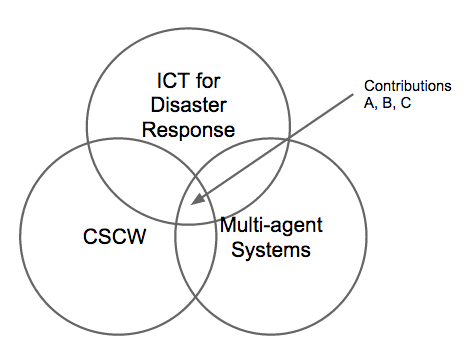
\includegraphics[scale=0.5]{img/introduction/contributions.png}
  \caption{Contributions}
  \label{fig:contributions}
\end{figure}

This thesis contributes to the knowledge in the following areas (Figure \ref{fig:contributions}): \\

\begin{enumerate}
  \item[A] \textbf{The system prototypes.} Real-world interactive prototypes (i.e. AtomicOrchid) for investigating human-system interaction in a disaster response setting. An iterative prototyping process is conducted throughout the three AtomicOrchid studies, which results in interactive prototypes of planning support systems. 
  
  \item[B] \textbf{The interactional issues.} The field observation of serious game trials generate thick descriptions of human system interaction in the collaborative work settings of \ac{DR}. The key observations reveal interactional issues surrounding automated planning support.
  
  \item[C] \textbf{Design implications.} For each study, field observations are further analysed to generate design implications which contribute to future deployment of automated planning support system in the complex collaborative work setting of \ac{DR}. 
\end{enumerate}


\section{Publications of this thesis} 
Parts of the contents of this thesis have been accepted by peer-review for publication in journal and conference proceedings in the field of \ac{HCI} and multi-agent system or are in submission. The core contributions include: \\


\begin{enumerate}
\item The chapters \ref{ch:approach}, \ref{ch:methodology}  present the approach and methodology employed to study interactional issues of planning support system. Some of the ideas of these chapters expands on the contents in:\\
\texttt{ \footnotesize Fischer, Joel E., \textbf{Wenchao Jiang}, and Stuart Moran. AtomicOrchid: a mixed reality game to investigate coordination in disaster response." In Entertainment Computing-ICEC 2012, pp. 572-577. Springer Berlin Heidelberg, 2012.}\\

\item The exploration of requirements for building coordination support system in chapter \ref{ch:studyone}  has been published in:\\
\texttt{ \footnotesize Fischer, J.E., \textbf{Jiang, W.}, Kerne, A., Greenhalgh, C., Ramchurn, S.D., Reece, S., Pantidi, N. and Rodden, T. (2014). Supporting Team Coordination on the Ground: Requirements from a Mixed Reality Game. To appear in: Proc. 11th Int. Conference on the Design of Cooperative Systems (COOP 14). Springer.}\\


\item The exploration of interactional issues related to human ``On the loop'' pattern reported in chapter \ref{ch:studytwo} has been published in:\\
\texttt{ \footnotesize\textbf{Jiang, W.}, Fischer, J.E., Greenhalgh, C., Ramchurn, S.D., Wu, F., Jennings, N.R. and Rodden, T. (2014). Social Implications of Agent-based Planning Support for Human Teams.  In: Proc. of the 2014 Int. Conference on Collaboration Technologies and Systems (CTS 14). IEEE.}


\end{enumerate}

Other contributions include:

\begin{enumerate}
\item Some results from studies in chapter \ref{ch:studyone} and \ref{ch:studytwo} also appeals in the journal article:\\
\texttt{ \footnotesize Ramchurn, S. D., Wu, F., Fischer, J. E., Reece, S., \textbf{Jiang, W.}, and Roberts, S. J., et al. (2015). Human-agent collaboration for disaster response. Journal of Autonomous Agents and Multi-Agent Systems.}\\

\item The game probe `AtomicOrchid' built in this PhD work is a central component of HAC-ER (Human Agent Collectives for Emergency Response) system  developed as main demonstrator of ORCHID project (orchid.ac.uk). The demonstrator is presented in the paper:\\
\texttt{ \footnotesize Ramchurn, S. D., Simpson, E., Fischer, J. E., Huynh, D. T., Ikuno, Y., Reece, S., and \textbf{ Jiang, W.} et al. (2015). HAC-ER: A disaster response system based on human-agent collectives. In AAMAS-15 : 14th Int. Conf. on Autonomous Agents and Multi-Agent Systems.} \\ 

\item The planner agent integrated in `AtomicOrchid' is based on a novel multi-agent coordination algorithm. Evaluation of the algorithm is partially facilitated the 'AtomicOrchid' trials:\\
 \texttt{ \footnotesize Wu, F., Ramchurn, S. D., \textbf{Jiang, W.}, Fischer, J. E., Rodden, T., and Jennings, N. R. (2015). Agile Planning for Real-World Disaster Response. In International Joint Conference on Artifical Intelligence.}

\end{enumerate} 

\section{Structure of the Thesis}
This thesis is structured as four parts. Part I surveys the relevant background literature. Chapter \ref{ch:literatures} will firstly give an overview of task planning activities together with command and control structures of \ac{DR} teams, followed by a review of empirical studies related to command and control work settings. The Chapter \ref{ch:literatures} then examines the state-of-the-art technology practices from 3 perspectives including planning support systems, \ac{ICT} support, and application of Artificial Intelligence in \ac{DR}. In Chapter \ref{ch:humanSysRelationship}, the relationship between technological support and human operators will also be examined by reviewing relevant literatures of \ac{CSCW} systems, Automation design and Human agent interactions. The rest of the chapter give an overview of serious mixed reality games which underpins the research approach of this PhD work.\\

Part II develops the approach and methodology employed to study interactional issues with planning support system in two chapters. Chapter \ref{ch:approach} develops the framework of interaction patterns under which interactional issues can be explored. The rest of this chapter introduces serious mixed reality game as approach to study interactions, followed by detailed description of the game used as testbed for this study, AtomicOrchid. Chapter \ref{ch:methodology} describes the methodology used to study the interactional issues. In particular, this chapter describes ethnographic observation and interaction analysis, which is supplemented by interviews. \\ 

Part III presents observational studies of this thesis. Chapter \ref{ch:studyone} reports the first observational study with AtomicOrchid. This version of AtomicOrchid does not have planning support agent included. The study establishes baseline human performance of task planning and derives general requirements of communication support. The Chapter \ref{ch:studytwo} gives an account of the second observational study of AtomicOrchid. In this study, a planning agent was built into the game with the human-on-the-loop interactional arrangement. Chaper \ref{ch:studythree} reports the third field study of AtomicOrchid with the human-in-the-loop arrangement. \\ 

The Part IV chapter \ref{ch:conclusion} concludes this thesis with a summary of discoveries, contributions, limitations and future work.\\










\cleardoublepage
\ctparttext{You can put some informational part preamble text here. }
\part{Background}
%*****************************************
\chapter{Task planning in disaster response}\label{ch:literatures}
%*****************************************
The overarching background of this thesis is disaster management, of which the \acf{DR} is one particular period immediately aftermath the disaster impact. This chapter reviews the research areas that are related to design and development of task planning support system for \ac{DR}. First, the section \ref{sec:lrplanning} reviews the relevant literatures to develop an understanding of planning practices in DR operations. In particular, the task planning activities in \ac{DR} operations are mostly embedded in a \acf{C2} environment. The section \ref{sec:LRC2} reviews the relevant empirical studies to gain insight into characteristics of \ac{C2} work setting. Second, practitioners have developed various technology support systems for disaster response. The section \ref{sec:LRApplicationAreas} gives an overview of technical practices in \ac{DR} in the context of three detailed application areas, which includes \acf{GIS} based planning support, \acf{ICT} systems and AI-based technologies. Third, empirical studies of technologies in use have showed that the ill-designed technology support may have negative impact on human workflow. \\

% The author believe this PhD work can contribute to bridging of two gaps identified in the literatures.
% Firstly, The DR task planning support sits in an unexplored gap between other related technology application domains. Now days, advances in information and communication technologies (ICT)  have brought increasing number of networked computers, sensors and the vast amount of data are generated from different sources during DR, in real time. Artificial Intelligent (AI) researchers have also devised lots of intelligent algorithms which enable computers to process real time data and make sense of the disaster environment. Arguably, the technological advances have created opportunity space for task planning support in DR, but the real world system in this domain are still rare. Although traditional computational support for planning has been studied for decades in various application domains, further research for the DR planning support are still required for addressing specific challenges raised from DR domain such as time pressure and uncertainty handling. \\

% Secondly, before we can develop an useful task planning support, the issues related to socio-technical gap may need to be examined. When introducing technological systems to support organisational work, researchers can often observe a divide between social and technical aspects within the organisation, which often cause negative on organisational performance. DR operations are also complex organisational work which requires highly coordinated team working. Therefore, we might need to examine impact of technological support on the social aspects of teamwork when we try to introduce task planning support for DR teams.\\

\section{Task Planning in Disaster Response}\label{sec:lrplanning}
To scope the task planning activities in \ac{DR}, this section begins with a definition of disaster response, followed by a brief overview of command and control structures of \ac{DR} organisations. The last section (\ref{sec:LRtaskplanning}) examines the main characteristics of task planning in large scale disaster response.\\

\subsection{Define disaster response}
Different countries and agencies may apply different rules and standards for defining phases of disaster management, but most of them agreed the disaster management is carried out in a circle. Figure \ref{fig:drCircle} illustrates the a model of disaster management cycle described in the literature \cite{Wattegama2012} :\\

\begin{figure}[h]
  \centering
  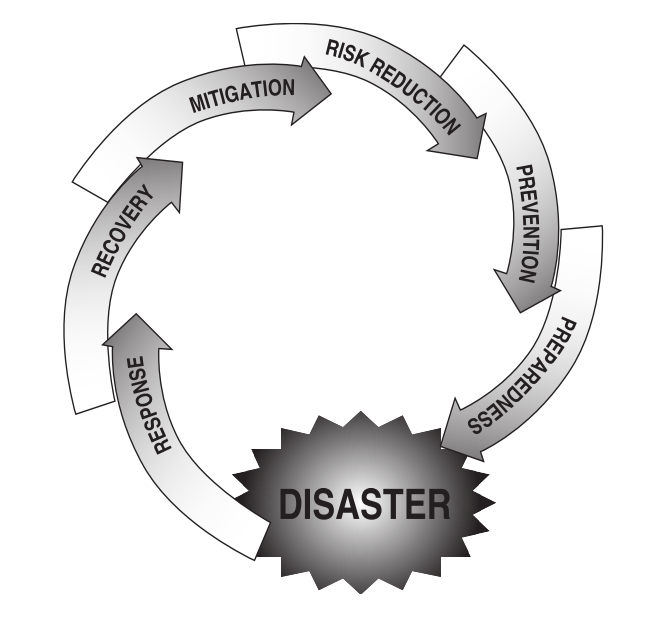
\includegraphics[width=1\textwidth]{img/background/drCircle}
  \caption{Disaster Management Circle. Credit \cite{Wattegama2012}}
  \label{fig:drCircle}
\end{figure}

\begin{enumerate}
\item Mitigation: any activity that reduces either the chance of a hazard taking place or a hazard turning into disaster.
\item Risk reduction: anticipatory measures and actions that seek to avoid future risks as a result of a disaster.
\item Prevention: avoiding a disaster even at the eleventh hour. 
\item Preparedness: plans or preparations made to save lives or property,and help the response and rescue service operations. This phase covers implementation/operation, early warning systems and capacity building so the population will react appropriately when an early warning is issued.
\item Response: includes actions taken to save lives and prevent property damage, and to preserve the environment during emergencies or disasters. The response phase is the implementation of action plans.
\item Recovery: includes actions that assist a community to return to a sense of normalcy after a disaster.
\end{enumerate}

The \ac{DR} operations refer to the actions taken during or immediate aftermath of the disaster strike. In this period, a significant number of individuals may be trapped and injured. Great number of structural damages need be dealt with. Medicine, food and shelters are in great demand. This period calls for prompt action within an exceptionally short period of time \cite{Wattegama2012}. Responder team may find themselves with limited resources and need to make plans to utilities the resources in a timely and satisfactory manner \cite{Chen2005,Chen2008}. \\

%\subsection{Team coordination in disaster response}
%Malone (1990 361) defines coordination as the act of managing interdependencies between activities performed to achieve a goal. One of the very important component of coordination in DR, following sections will firstly... and then discuss how the coordination is carried out through command structure of DR team. \\

%In disaster response, team coordination is essential in order that groups of people can carry out interdependent activities together in a timely and satisfactory manner (cf. Bradshaw et al., 2011). Disaster response experts report that failures in team coordination are the most significant factor in critical emergency response (Toups et al., 2011: 2) that can cost human lives. Shared understanding, situation awareness, and alignment of cooperative action through on-going communication are key requirements to enable successful coordination. Convertino et al. (2011) design and study a set of tools to support common ground and aware- ness in emergency management. \\

\subsection{DR command structure}\label{sec:lrstructure}
The emergency response agencies typically employs a hierarchical command structure \cite{Ramchurn2015}. One widely used command and control structure the Gold, Silver, Bronze model. In this model, decision making is divided into strategic, tactical, and operational levels. The teams responsible for each are referred to as ``Gold, Silver, and Bronze'' respectively. The decisions on main objectives of the response effort are made at the strategic (Gold) level. At the tactical level, the Silver command team decides on the allocation of resources and tasks to be carried out  based on the specified objectives. At the operational level, Bronze first responders (FR), on the ground, determine the logistics required to carry out those tasks. Information gathered from the ground is also passed back up from Bronze, through Silver, to Gold \cite{Ramchurn2015}. Some literatures \cite{Chen2005,Chen2008} also generalized the command and control structures as a generic two level model. The key characteristic of the two-level model is division between remote coordination center and on site teams.  On-site responders react to immediate scene without global picture, while the coordination center deals with strategic issues and works with a global picture, leveraging external resources to help on-site response. \\

%insert picture 

\subsection{Task planning in large scale disaster} \label{sec:LRtaskplanning}
One important characteristic of large-scale disaster is the presence of multiple spatially distributed incidents \cite{Chen2005}. To gain insight into the problem of task and resource allocation in large scale disaster, we will firstly examine how a single incident is dealt with. The procedures of dealing with single emergency incident have documented by a number of field studies \cite{Comfort2004,Dawes2004,Petrescu-prahova2005}. In Toups's \cite{Toups2011} study, fire emergency response to small-scale structural fires is depicted as follow: 

\begin{quote}
Fire emergency response is undertaken by small teams distributed throughout the incident, coordinated by an incident commander (IC) . Multiple response teams, or companies, are dispatched to any incident and cooperate around the fireground. A company officer leads each team, which consists of firefighters and/or engineers.2 Normally, each company is associated with a firefighting vehicle; an apparatus, such as an ambulance, engine, or ladder truck.\\
\end{quote}

From the depiction of single incident emergency response, we can see that a combination of different resources (e.g. ambulance, fire engine, ladder truck ) and skills (e.g. structural engineers, firefighters and medics) are deployed to the location of the incident. To deal with multiple incidents, the disaster response team has to coordinate spatially distributed resources and personnel to carry out operations (e.g. search, rescue and evacuation) \cite{Chen2005}. That is , resources and responders needed to be divided and combined in to teams and deployed to handle distributed incidents. Depending on the number of incidents, response personnel may need to dispatch, deploy and redeploy limited resources. One major concern for task planning in disaster response is how to efficiently allocate limited resources to multiple incidents with temporal and spatial constraints \cite{Bradshaw2011}.\\

Also, the task environment of \ac{DR} is characterised by various uncertainties including, but not limited to hazard uncertainties, task-flow uncertainties, environmental and informational uncertainties \cite{Chen2008}. Sudden and unexpected events may occur as the disaster situation unfolds. Therefore, fixed plans of actions for responders is unlikely to work. The uncertainties may need to be handled by improvisation, prioritisation, and dynamic sourcing of capabilities \cite{Faraj2006}, which means dynamic change of plans is necessary to deal with uncertainties in dynamic task environment.\\   

In summary, responders in \ac{DR} need to carry out a set of interdependent activities under time pressure and spatial constraint. Both their resource (personnel and physical assets) and capacity of problem solving required for planning may be stretched in a large-scale, multi-incident disaster. To alleviate the problem, technological support in \ac{DR} has long be studied by computer scientists. We will review some of the related research areas in next section.\\


%geo-distribution and time pressure has been identified as challenges for task planning and execution. Uncertainty new means real time and dynamic task planning[chen's emergency response]. Geo distribution creates uncertain in the information [short distributed team paper][the human factor in dr paper discussion failure of communication] and creates time constraint as well because teams need to be  \\


%chen's emergency response some practitioners articles

%The fireground and surrounding space constitute a dangerous and dynamic interface ecosystem [Kerne 2005] of distributed cognition, connecting responders, victims, fire- fighting equipment, communication media, and information artifacts. Upon arriving at an incident, multiple companies distribute in and around the fireground. Compa- nies and their apparatuses are placed at strategic locations, and are moved as needed. Human operators work on and from these platforms. Firefighters and rescue workers deploy from them, taking equipment into the fireground; equipment, such as firehoses and radios, may be technologically supported by the apparatus itself (pumps and water sources, or high-power repeaters, respectively). Each apparatus, and in many cases, each human worker, is equipped with a half-duplex radio to facilitate long-range, broad- cast communication.\\

\section{Command and Control Environment}\label{sec:LRC2}
The \acf{C2} environment have been a long standing research topic in the field of \acf{HCI}. The  research of \ac{C2} setting focuses on how operators manage and control safety-critical systems \cite{Fischer2015}. The studies of \ac{C2} work setting is particularly relevant to this thesis, because most emergency response operation is carried out in a \ac{C2} environment (section \ref{sec:lrstructure}). \\

In the field of CSCW, ethnographic studies are carried out to explicate work practice and organisational conduct in the \ac{C2} environment, with the aim to inform the design of technological support systems. The studies are conducted in a range of application areas such as air traffic control \cite{RichardH.R.HarperJohnA.Hughes1989}, emergency response \cite{Fischer2015} , and military operations \cite{Tolcher2005}, with the aim to provide design implications for technological support. For example, the The work of \cite{Heath1992} conducted a detailed examination of social organisation of collaborative work within a line control room in London underground. The analysis of \cite{Heath1992} particularly focus on interaction between different personnel as they coordinate a range of tasks and utilise various tools. The study revealed the methodological ways in which the participants surreptitiously monitor each other's conducts, and at the same time, render their actions visible and accountable to the other team members. Therefore, it is critical for computational systems to facilitate individuals mutually to monitor their co-participants \cite{Heath1992}.\\

Similar \ac{C2} setting can also be found in the orchestration of \acf{MRG} experiences in which online players in the control room and field players `on the ground' interacts through pervasive technologies such as smart phones, GPS and other mobile sensors (Section \ref{sec:LRMRgame}). The ethnographic studies of MRGs \cite{Benford2006}, \cite{Crabtree2004}, \cite{Koleva2001} focus the distributed natural of \ac{C2} environment. The observations in the studies reveal methodological ways in which players collectively battle the uncertainties and interruptions of technologies through distributed orchestration process. The results of the studies leads to a set of design implications for handling uncertainties and interruptions in the distributed \ac{C2} environments. \\

Apart from ethnographic studies, the impact of technology support in the control room is also assessed by human factor researchers through quantitative evaluation of operators' performance \cite{Grootjen2007}, \cite{Sharples2011}. For example, the study by \cite{Sharples2011} is conducted to assess impact of recent automation in rail way signalling operations. The studies evaluated changes of operators' performance through statistical test and quantitative comparison of observational data. The results indicate that automation is effective at reducing high level of interaction and workload. However, operators do seem to struggle to maintain awareness of system state and that they are also unable to monitor the way in which automated support makes decisions in real time. \\

While both qualitative and quantitative studies contribute to understanding of human-system interactions in complex \ac{C2} settings, this PhD work is primarily interested in understanding of social organisations of work, and follow the tradition of empirical \ac{CSCW} studies to unpack the social interactions in \ac{C2} setting. \\

%The analysis is no longer primarily concerned with the individual and the system, but rather the  The ability to coordinate activities, and the process of interpretation and perception it entails, inevitably relies upon a social organisation; a body of skills and practices which allows different personnel to recognise what each other is doing and thereby produce appropriate conduct. Heath and Luff's study of London Underground shows for example how co-orientation among operators is critical in this ``multimedia environment''.\\


\section{Technological Practices in Disaster Response} \label{sec:LRApplicationAreas}
So far, we have framed the problem of task planning in \ac{DR} in section \ref{sec:lrplanning} and reviewed three research domains related to development of \ac{DR} planning system in this section. To give an overview of current technological practices related to planning support, This section will reviews three related research domains in the context of computational DR support, that is - \ac{GIS}-based task planning systems for plan formulation and evaluation ; \acf{ICT} for information acquisition and management; and the \acf{AI} technologies for disaster simulation, and plan optimisation.  \\

This PhD work is primarily interested in a real-time task planning system that utilise \ac{ICT} technologies as its underlying infrastructures and apply intelligent coordination algorithms for plan generation. This kind of system can be located in the overlapping area of the three research domains that is reviewed in this section (see figure \ref{fig:SystemFraming}).\\

\begin{figure}[h]
  \centering
  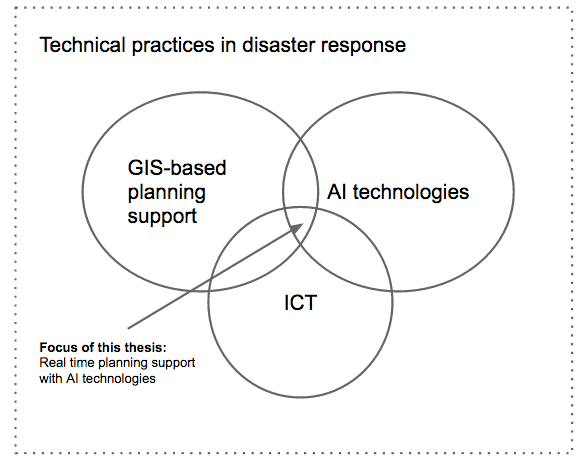
\includegraphics[width=1\textwidth]{img/background/SystemFraming}
  \caption{technological support for disaster response}
  \label{fig:SystemFraming}
\end{figure} 

\subsection{GIS-based planning support systems}
The \acf{PSS} can be defined as a suite of computational components that help planners to explore and manage planning activities \cite{Geertman2004}.Literatures have documented a variety of planning support systems with a range of purposes such as land development \cite{Pettit2003}  and logistic scheduling \cite{Miller}. In the context of disaster response, planning activities  typically concern dispatch, routing and deployment of rescue resources (see section \ref{sec:LRtaskplanning}), which means the \ac{GIS} for spatial analysis may be a central component of a planning support suite. Therefore, this section will focus on reviewing the \ac{GIS}-based \ac{PSS}. \\

While the general-purpose \ac{GIS}  are only designed to handle geo-spatial data \cite{Geertman2004}, the PPS may have a wide variety of functionalities to support multiple aspects of planning process, which may include, but not limited to problem diagnosis, data collection, mining and extraction, data modelling, visualisation and display, scenario-building and projection, plan formulation and evaluation, and collaborative decision-making support \cite{Geertman2004,Zerger2003}. A range of the \ac{GIS}-enabled planning systems have been developed for various purposes such as vulnerability assessment, risk management and hazard mitigation \cite{Cova199,Schooley2010}. One example is the ``Intergraph'' developed by Victorian Emergency Services (Australia) \cite{IntergraphCorporation2000} to support emergency dispatch services (e.g. ambulance, police and fire services). The system support daily response activities by providing automated geo-referencing, routing, mapping, planning and analysis \cite{Zerger2003}. Another example of \ac{GIS}-based planning support is an evacuation planning tool for radiological disasters developed by \cite{Eglese1994}. The system combines simulation models and  \ac{GIS} software to model evacuation routes for evacuation in radiological incidents.  It uses the spatial data structure and programmed simulation models to predict traffic flow through the road network under scenarios such as vehicle breakdowns and road closures. The system is designed for evaluation of evacuation strategies prior to disaster. Real-time decision support is not possible because the simulation is computationally intensive.\\

The `real time' task planning in \ac{DR} is different from other long-term planning scenarios due to time pressure and uncertainties involved.  Responders in DR have to plan dynamically according to the disaster environment that are always quickly changing. The study of \cite{Zerger2003} have pointed some technical and social impediments for applying \ac{GIS} tools to support `real-time' planning activities in DR. First, some spatial modelling and simulation technologies can be very (such as \cite{Eglese1994} ) computational intensive which makes it unable to provide results in real-time. Second, some of the planning systems are adapted from \ac{GIS} software, which require high level of training to operate. Third, there are lack of social and organisational considerations in the most of existing \ac{GIS} tools. For example, some PPS are based on a single computer terminal, which is unable to facilitate information sharing with multiple users in control room and `on the ground'. \\

The third point is aligned with the studies of \ac{C2} task environment (in section \ref{sec:LRC2}). The C2 environment is collaborative setting which involves complicated social interaction and organisational conducts. Therefore, the PPS designed for \ac{C2} environment should consider supporting the social conducts of responder teams. Further, the computational support in modern \ac{C2} environment (e.g. air traffic control \cite{Mercer2014} and underground control \cite{Sharples2011}) supports a range of activities such as information acquisition, analysis, decision selection and action implementation. Similar to other \ac{C2} environments, plan generation and action implementation in DR are typically fast pace and happens in parallel. The existing PPS such as \cite{IntergraphCorporation2000}, \cite{Eglese1994} only provide isolated functionalities for supporting plan generation. To realize `real-time' planning support, the author believes the PPS should be further extended or integrated with other system functionalities for action implementation, such as progress monitoring, conflict detection, and communication support.\\

%Efforts have been made to study and design such real-time task planning system for DR Wagner et al. [2004]; not Okaya et al. [2014], but the real deployments are still rare.[Bring up the previous ] Once we extend the capabilities planning system with real-time capabilities, the boundary between planning system and command/control systems (e.g ground traffic and aviation control \cite{Sharples2011}) are blurred. In this PhD work, we will call the system sitting in the middle ground area `real time planning' system. Some researches treat command and control system as tools to automate some aspects of command control activities including information acquisition, analysis, decision selection and action implementation \cite{Sharples2011}.  In contrast, a `real-time planning support system' may have stronger focus on supporting real-time plan generation and selection.

\subsection{ICT support for disaster response}
The \acf{ICT} includes communication infrastructures and software system on top of the infrastructures. The communication infrastructures refer to communication channels such as radio, television, satellite, internet, text and voice communication over mobile phone. The basic communication infrastructures have long be utilised by responders to capture both soft data (generated by human) and hard data (from sensors) for their decision making \cite{Fischer2012}. Apart from the infrastructures, the \ac{ICT} software systems are playing increasingly important role. Now days, most DR practice may consists  of both the manual processes which directly relies on \ac{ICT} infrastructures and the automated (or partially) process of data analysis and information management that are supported by \ac{ICT} softwares. For example, the figure \ref{fig:ICTExample} illustrate a tsunami response system operated by Asian Disaster Preparedness Center(ADPC) \cite{Wattegama2012}. In this system,  the technical components are comprised of a network of seismographic stations, sea-level gauges and deep-sea pressure sensors. A tsunami forecasting centre is equipped with seismic processing and modelling software.  Tsunami warnings are disseminated through the communication links between national centres and the people at risk, the links include, email, television, radio, cellphones and satellites. Another scenario for \ac{ICT} support can be found in most modern \acf{ERR}. For instance, the ERRs in Amsterdam uses a \ac{ICT} software called GMS (Integrated Emergency Response Room System) \cite{Boersma2009}. GMS is used to connect the different information sources (e.g. a national digital radio network for public safety). However, the \ac{ERR} in Amsterdam is not co-located, but divided by regions and functions (Fire,Police and Medical). GMS used by \acf{ERR}s are not connected and they are tailored differently to the various needs and requests of operators. As the \acf{ERR} systems are disconnected, information exchange between \ac{ERR} is conducted manually through telephones \cite{Boersma2009}.\\

\begin{figure}[h]
  \centering
  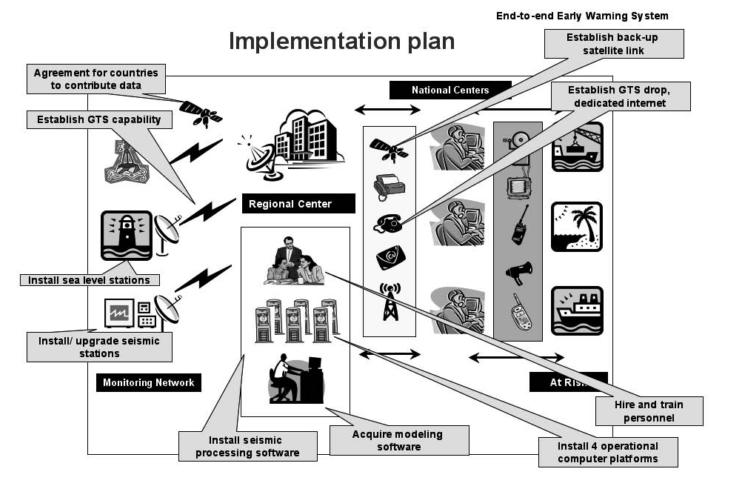
\includegraphics[width=1\textwidth]{img/background/ICTExample}
  \caption{Tsunami response system, Credit \cite{Wattegama2012} }
  \label{fig:ICTExample}
\end{figure}

With proliferation of smart phones and ubiquitous computing technologies, internet have become increasingly important in the disaster response. Web-based applications have been used in the indian ocean tsunami for tracking missing people, coordinating donors, and recording locations of shelters \cite{Wattegama2012}. The internet also expanded the possibilities for public participation. For example, the use of microblogging tools such as `twitter' in \ac{DR} have have been a popular research topic in the field of crisis informatics \cite{Kogan2012,Sarcevic2012,Starbird2010}.  The microblogging tools enabled the public to take not only a more active part in seeking information, but also in providing information to each other, as well as to formal response efforts. Crowedsourcing platform such as Ushiadidi \cite{Morrow2011} is another example of \ac{ICT} support for public participation in \ac{DR}. The Ushiadidi platform have been used in the Haiti earthquake as a volunteer effort to produce a crisis mashup. Information about the humanitarian crisis and the response that followed was aggregated in near real time by volunteers from a variety of sources including: SMS, Web, Email, Radio, Phone, Twitter, Facebook, Television, List-serves, Live streams, Situation Reports \cite{Morrow2011}. Similarly, crowedsourced map systems such as OpenStreetMap \cite{Palen2015} have been applied in disasters (Haiti earthquake, Typhoon Yolanda) for volunteers to create updated crisis map. Although public participantion has played an important role in \ac{DR}, its integration with formal response efforts is still a challenge for \ac{ICT} researcher \cite{Palen2007}, and a lot of research efforts have been made to address social, organisational and technical challenges of the integration \cite{Dashti2014}, \cite{Sutton2008}.   \\

In summary, \ac{ICT} infrastruce and software are commonly used in disaster response. Two case studies (tsunami response system and emergency response room support) are used to illustrate the \ac{ICT} supported DR processes. Public participation is another trend of \ac{ICT} system support raise from increased global access to internet. However, studies showed integration of public participation and formal response efforts is still problematic and require further research. From the author's point of view, a task planning support may heavily rely on \ac{ICT} infrastructure for data acquisition and plan implementation. Functionalities of \ac{ICT} software also have many overlaps with that of task planning systems, in the sense that they all support responders to acquire, process and manage information for the use of decision making in \ac{DR}. \\


\subsection{Application of AI technologies}\label{sec:lraisupport}
In the field of \ac{AI}, machine learning, optimisation and agent-based simulation algorithms have increased in availability for disaster response. \\

Disaster simulation technologies \cite{Okaya,Scerri2005} have long been applied in various types of disasters such as fire \cite{Tang2012}, hurricane \cite{Vickery2009} and earthquake\cite{Sobhaninejad2011} to understand the process and impact of disasters. The state of art simulation technologies are able to provide real time simulations with high data resolution. For example, the simulation platform devised by \cite{Sobhaninejad2011} is able to provide real-time simulation of ground motion and structural damage after earthquake, in an urban area with {1e4} to {1e6} structures. \\

Evacuation simulation is also extensively studied in the literatures. For example, \cite{Pillac2015} developed a simulation algorithm for large scale flood evacuation. The algorithm consider the dynamics of the flood and the state of the transportation network over time. The experiment showed this algorithm is able to provide plans to evacuate about 70,000 people in a impact region in real time.  Another example can be simulation of indoor fire evacuation devised by \cite{Tang2012}.  The algorithm combines modelling of building geometry, human behaviour, fire field to provide intelligent decision support. While results of evacuation simulations are promising in lab experiments, some studies pointed out the simulation technologies over simplified the human behaviours \cite{Hentenryck2011}. For instance, in some countries, most people disregard evacuation orders. The complexity of human behaviour raise from cultural, political, psychological factors, which makes behaviour modelling a challenging topic for \ac{AI} community \cite{Provitolo2011} . \\

%Apart form disaster simulations, optimisation algorithms have been studied for resource allocation in DR [][]. The model use detailed descriptions of operational areas such as xxx,xxx,xxx and available resources to caculate the resource performance and efficiency for different tasks related to the response. It is important to deliver water, food, medicine, and other commodities .\cite{Fiedrich2000} ties as quickly as possible after a disaster strikes. For a partic- ular commodity (or collection of commodities), the problem consists in deciding 1. where to store the supply and in how much quantity; 2. how to deliver the commodity as far as possible. The first question is strategic or tactical in nature; the second one addresses the response. The overall problem is stochastic and the goal is to minimize a lexicographic objective function consisting of minimizing the unsatisfied demand, the latest delivery time, and the storage costs, using eith stochastic or robust optimization. The second objective, which is unconventional, was a DHS requirements and differs from traditional objective functions in vehicle routing which often aim at minimizing travel distance or cost. \\

Agent-based optimisation algorithm for multi-agent teams coordination is also an active research area in \ac{AI} community. The coordination challenges in the time critical task environment inspired the multi-agent researchers to investigate real-time algorithms that provide optimal or near optimal task plans that can be used to guide distributed human or robotic teams \cite{Kitano2000}. Various algorithms have been designed to meet different requirements of team coordination. For example, the \cite{Lagoudakis2005} provide a number of auction-based algorithm that allocate agents to tasks considering the best routes for each agents in the team. On the other hand, \cite{Scerri2005a} devised algorithms to allocate tasks based on token passing. Their algorithms focus on matchings of task and team capabilities, which ensures that the right agents are routed to the right tasks based on capability thresholds. Other algorithms \cite{Ramchurn2010,Koes2005} also consider multiple criteria including task workload, deadline and team coalition effects. From \ac{HCI} perspective, these capabilities of these algorithms are also limited by a number of factors. First, the concerns about oversimplified human behaviour modelling is applied \cite{Drury2009}. Second, because the algorithms are designed to deal with specified requirements (e.g. routing, task/skill matching) with simplified model of environments, they may be insufficient to deal with contingencies raised from messy real disaster environment \cite{Armenakis2012}.\\

It is observed that most intelligent algorithms are only studied and evaluated in the research lab. Integration of the algorithms and actual\ac{DR} practices is still a multi-disciplinary research challenge. Nowdays, with the increase in the networked computers, sensors and amount of data generated from different sources in real time \cite{Ramchurn2015}, there are increasing demand for intelligent computational support of data processing and task planning. As a case study, researchers from ORCHID project have developed a prototype system - HAC-ER (Human Agent Collectives for Emergence Response) \cite{Jennings2014,Ramchurn2015,Ramchurn2015a}, which demonstrates how the \ac{AI} algorithms may transform the landscape of real time task planning in \ac{DR}.\\

The \ac{HAC-ER} system consists of a set of connected components for real-time task planning support, each of which are powered by multiple machine learning and agent-based algorithms. First, a component called Crowedscanner is used to deal with vast quantities of unstructured data produced very rapidly on the internet as disaster unfolds, such as text messages or photographs from web-based platforms such as Twitter and Ushahidi \cite{Morrow2011}. The approach is to use a machine learning algorithms (for details, see IBCC \cite{Simpson}) to fuses heterogeneous reports from both unreliable and trusted sources into a common picture of the disaster, or a heatmap of incidents. Second, multiple  \acf{UAV}s is deployed as mobile sensors to search or further inspect incidents reported by crowdscanner. The control of multiple \ac{UAV}s is assisted by multi-agent coordination algorithm (Max-sum \cite{Ramchurn2010}). The algorithm is capable of quickly optimise the task allocation for \ac{UAV}s to visit points of interest or conduct search in an area.  Finally, responders and assets on the ground will need to be dispatched and deployed to deal with distributed incidents. Another \ac{HAC-ER} component is designed to assist human operators in the control room to conduct real-time planning. The component is powered by a coordination algorithm based on MMDP modelling techniques \cite{Wu2015}, which takes into to account the priorities of incidents, and locations of responders teams and incidents. The algorithm can produces computationally optimised task allocations for responder teams to attend as many incidents as possible with a time constraint. Further, algorithms and interfaces of all components in \ac{HAC-ER} are designed in a way that accept input form human operators. The \ac{HAC-ER} depicted a picture in which human operators and intelligent components collaboratively conduct task planning, and the picture demonstrates the potential for applying \ac{AI} in \ac{DR} task planning.\\

\subsection{Summary}
This section have reviewed technological practices related to planning support in disaster response. First, there are great many \ac{GIS}-enabled \acf{PSS}. However impediments for applying the \ac{GIS}-based are also identified in literatures. For example, \ac{GIS} planning system with real-time capabilities are rare and there is also lack of social and organisational consideration in the design of \ac{GIS} planning systems. Second, the \ac{ICT} infrastructures and softwares have long be utilised by responders for managing communication and information. The author believe \ac{ICT} provides the basis for real-time task in the sense that it provide functionalities to support information acquisition and management. Finally, \ac{AI} researcher have devised some machine learning and agent-based algorithms to support task planning. Prototype systems have been built to demonstrate the potential for planning support based on \ac{AI} technologies.\\ 

In the overlapping area of the three application domains, there is an opportunity space for real time task planning support in \ac{DR} domain. The planning support system can utilise \ac{ICT} technologies as its underlying infrastructures and apply intelligent coordination algorithms for plan generation. However, the literatures for building such a system are still rare, leaving a gap in literatures. This thesis is aimed to bridge the gap by studying the design and development of such \ac{DR} planning support system.\\

\section{Summary}
Relevant literatures have been reviewed in this chapter. The studies of disaster response operations showed that the task planning activities is challenging due to time, spatial constraints and uncertainties in dynamically changing disaster environment. Further, the \ac{DR} planning process is typically embedded in a \acf{C2} task environment. The literatures have revealed that the \ac{C2} setting is characterised by complex social interaction and organisational conducts. Therefore, technology support do not only need to provide the solution of complex coordination problems, but also need to support social aspects of planning generation in complex \ac{C2} setting. \\

There are various existing technology support designed for \ac{DR}. First, the \ac{GIS}-based planning support \ac{GIS} functionalities with environmental modelling techniques to provide decision support for various purposes such as floor and indoor fire evacuation. However impediments for applying the \ac{GIS}-based are also identified in literatures. For example, most \ac{GIS} planning system can not support real time decision making and there is also lack of social and organisational consideration in the system design. Second, the \ac{ICT} support system historically played an important role in \ac{DR}. Now days, the \ac{ICT} infrastructures and software are becoming increasingly connected at global scale, which changes the landscape of \ac{DR} by expanding the possibilities of public participation. Further, the \ac{AI} community have also devised various machine learning and optimization technologies for \ac{DR} operations. Particularly, a number the multi-agent coordination algorithm have been devised to provide solutions on task allocations in \ac{DR}. In the overlapping area of the three application domains, there is opportunity space for real time task planning support in \ac{DR} domain. While the The planning support system can utilise \ac{ICT} technologies as its underlying infrastructures and apply multi-agent coordination algorithms for plan generation. However, the researches for building such a system are still rare, leaving a gap in literatures.\\

\chapter{Interaction between Human and Planning support system}

Applying task planning to support complex disaster response operations may not be a straightforward process. Some HCI literatures \cite{Ackerman2000,Bowers1994,Niazkhani2009} have shown that introducing technology system to support organisational work may be extremely difficult. Use of technologies may have unexpected negative impact on human team performance. This thesis adopted a socio-technical view towards the undesirable impact of planning support technologies on human team performance. Particularly in planning support system, the socio-technical perspective concerns with issues the emerge form the gap between the human , system problem solving, namely the divide between a situated actions of human and cognitive planning model held by system [suchman]. Meanwhile, other two HCI researcher areas are particularly concerned with human system interaction. First, the research of automation design  concerns what and how to automate a working process by using computational systems. Second, the research of human agent interaction focuses on building software agent that is capable of teamworking with human operators. This section will review the three perspectives to give an conceptual background of design challenges that we may encounter when developing DR task planning support.\\

Further, studying human system interactions in real world disaster could be very challenging because disasters conditions can not be reproduced easily. Therefore, researchers have long been using gaming as an approach for studying the impact of technology support.  The section \ref{sec:LRMRgame} reviews the strengths and weakness of using game as an approach for studying disaster work setting. \\


\section{A socio-technical perspective to technology support} \label{sec:LRSocialTechnical}

A so-called socio-technical gaps that are often found in design and development of CSCW (Computer Supported Cooperative Work). The research field of CSCW addresses how collaborative activities can be supported by means of computer systems \cite{Carstensen1999}.  CSCW goes beyond building technology itself and investigates how people work within groups and organizations and the impacts of technology on those processes. The term socio-technical systems was originally coined by Emery and Trist \cite{Ropohl1999} to describe systems that involves complex interactions between humans, machines and the environmental aspects of the work system. The implication of this definition is that both social and technical factors e.g. people, machines and context need to be considered when developing such systems. Introducing a technology support system into an organization requires the technical and social aspects to be integrated, which can be a major challenge of building CSCW systems \cite{Ackerman2000}. \\

Researchers have recognised a so called socio technical gap in many CSCW systems. It is argued that \cite{Ackerman2000}  human activities is highly flexible, nuanced, and contextualized and that computational processes and entities such as information transfer, roles, and policies need to be similarly flexible. The social-technical gap is the divide between what we know we should support socially and what we can support technically \cite{Ackerman2000}, and the gap may result in serious negative impact on human activities. \cite{Bowers1994,Abbott1994a}. Therefore, it is vital to study technology in use to understand potential tensions between technical mechanism and social life \cite{Bowers1994}.  In the context of disaster response, we believe the same is true for the application of agent-based planning support. Empirical works \cite{Petrescuprahova2005,Kopena2008,Fischer2015,Zerger2003} have revealed the complexity of social and technological processes in disaster response operations. Responders with different roles have to engage in the various interdependent activities that are distributed in both time and space (see section \ref{sec:lrplanning}). To build agent-based systems that support human team coordination, exploration of such social-technical gap and its impact can be vital. \\ 

\subsection{The socio-technical gap for planning support system}
In the context of planning support, the socio-technical gap can be specifically originated from the different ways in which human and system plan and act. The view of purposeful action is adopted by many researchers and designers of intelligent systems, serving as the model of plan and action that is embedded in lots of problem solving systems \cite{Allen1984}. On this view, plan is a prerequisite of and prescribe to action. The view of purposeful action is also embraced by behavioural science as the basis for traditional view of rational human actions. However, the view of purposeful action is challenged by recent trends in sociology, arguing that prescriptive significance of plans and intentions for action is quite vague. Rather then determining the actions, the plans only serve as resource for human's practical deliberation about action \cite{Suchman1987}.\\  

\subsubsection{Planning model embedded in problem solving systems }
% The machine planning 
% The planning model, on which most system have been build on. Plan generation, replan, 
The view of purposeful action underpins the planning model form cognitive science. The planning model is embedded many of problem solving systems \cite{Suchman1987}. The model treats a plan as a sequence of actions to achieve an end goal. In problem solving systems, actions are described by prerequisites(The condition triggers action), effects (The condition after action) , and decomposition(Executing subactions) \cite{Allen1984}. The situation of action is the conditions that hinders the actors' movement to the end goal status. Some problem solving systems is only designed for plan generation. When a plan is constructed, the problem solves finished their work, assuming nothing will go wrong. However, contingent situations (or unanticipated conditions) will emerge, requiring  \cite{Suchman1987} replanning. Therefore, modern antonymous systems is typically designed to conduct planning and execution monitoring, which enable them to respond to contingent situations.\\

% figure

% Plan recognition to achieve xxx.
The recent development in artificial intelligence (e.g. multi-agent systems) requires the planning model to be extended from individual agent to multi-agent situation. To achieve concerted actions in the social situation with multiple agents, the planning model seeks to attach the knowledge of other agent's plans and actions as a type of environmental condition for planning. In this way, the basic view of single, goal directed agent (e.g. BDI model of agents \cite{Georgeff1999}) is remain intact. To obtain the knowledge of other agent's plans, agents are required to conduct plan recognition in addition to planning and execution monitoring. The basic assumption of plan recognition that agents as observers take actions of each other as evidence to form hypothesis of plans that explain intentions and actions of each other.  \\

The planning model is problematic when it is applied as model of human's ``psychological process'' of action. Studies have pointed out in many occasions human actions do not appear to follow logical steps or rational plans \cite{Suchman1987}. Researchers of cognitive science argued that the issue is due to actions under vague intents and incomplete plans. As a result, the human planning activity is often inferior version of scientific planning that need to be supported. However, many sociologists challenge the view by refuting the significance of plans in determining actions  \cite{Suchman1987}. The key argument arguing that the human action is essentially situated, not planned. This argument will be detailed in next section.\\ 

\subsubsection{Situated actions of humans}
% The human planning
% Situated actions, suchman argued it is what human follows
% Plan is just a representation of situated actions, and why it is always mistakenly treated as rational. 
In contrast to problem solving systems, recent efforts in sociology argue that human perform in . The argument adopts the view of situated action as oppose to the view of purposeful action held by AI researchers \cite{Suchman1987}. The starting point of argument is that the plan does not prescribe the actions. The plans are part of a large context of circumstance of ongoing actions, serving as a resource for deliberation on actions [ibid].\\

In the view of situated action, the plans are only representations of our actions in the form of imagined projection and recollected reconstructions, which does not have causal relation to the actions we take. Psychologists \cite{Mead1934} suggested, although a great deal of deliberation, discussion can be taken into the plan, our plans can stop short of our actual actions. And our post hoc analysis of situated actions often make it appears to have followed rational plans. \\

In contrast to plan recognition, mutual intelligibility in a social situation is not achieved by using logical formulae and formal algorithms based on behavioural observation. Instead, situated actions are highly dependent on specific occasions circumstances and social situations. Mutual intelligibility is sustained through every instance of interaction, rather than fixed social rules and constraints \cite{Suchman1987}.\\

% Situation is achieved 

\subsection{Summary}
The great divide between planning model embedded in many problem solving systems, and situated actions performed by humans signifies the issues of human system interaction in complex socio-technical systems such as disaster response management (Table \ref{tab:planningcontrast}). In contrast to fully autonomous system, computational support system have to interact with human to achieve mutual intelligibility and concerted actions. It is important to recognise the common sense planning activities of human is not a inadequate version of scientific planning model that need to be improved or supported by systems. Instead, human plans and acts in a way that is fundamentally different from machine problem solving. Therefore, a big challenge in designing technology support is how to bridge the socio-technical gap between situated action and scientific planning model.\\

\begin{table}[h]
\centering
\footnotesize

\label{my-label}
\begin{tabular}{l|ll}
                 & Plan                                                                                                                           & Interaction                                                                                                                                                                                               \\ \hline
Planning model   & \begin{tabular}[c]{@{}l@{}}Prerequisite of to and \\ prescribe to actions.\end{tabular}                                        & \begin{tabular}[c]{@{}l@{}}Shared understanding is achieved \\ through plan recoginition.\\ Plan recgnition is achieved by \\ logical formelae based on \\ observations of other's behaviour\end{tabular} \\
Situated actions & \begin{tabular}[c]{@{}l@{}}Do not prescribe actions.\\ Resource of deliberation \\ and Representation of actions.\end{tabular} & \begin{tabular}[c]{@{}l@{}}Mutual intelligently is achieved\\  through interactions embedded\\  in the social situations.\end{tabular}                                                                   
\end{tabular}
\caption{Planning model and situated action}
\label{tab:planningcontrast}
\end{table}
 
% (status of plan) The plan is essentially the simulation of actions

% Situated actions of human is inadaquate version of scientific plannning

% The gap  
% a table for contrasting 
% System is ok to follow, achieve a goal through comprehaisve search of solution space. It would be ok for fully autonmous. When in the situation of social technical system 

%For the purpose of designing usable and useful computer systems for cooperative work settings we need to know what makes work situations complex to competent actors and how computer systems may be of assistance to reduce or otherwise cope with this complexity. 

% Instructions 
% Human to Human
% Expert system


\section{Other perspectives of human system interaction}
Two HCI research areas, namely Automation design and Human agent interaction, are relevant to development of autonomous systems that collaborate with human. This section reviews literatures in these two areas, with the aim to further develop understanding of issues and challenges of human system interaction. \\


\subsection{Automation and its impact on human performance}
The aim of an automated support system is to replace the tasks originally performed by human with a machine. \cite{Bradshaw2011} . It can be defined as the execution by machine, usually computer, of a function previously performed by human \cite{Parasuraman1997}. The tasks that can be automated is used to be limited by technical capabilities, but this is no longer the case. With quick growth of machine's speed and intelligence, the tasks that can be automated is rapidly increasing, including complex cognitive activities such as information analysis, planning and decision making \cite{Parasuraman2000}. The boundary between human machine capabilities has blurred. The automation designers have to make hard choice about what to automate and to what extent.\\

One traditional approach for automation design is to simply automate all system functions that can be automated easily in a cost-effective way, leaving the all remaining tasks to human operators. The main considerations in this approach are technical capability and cost. The assumption of this approach is that the automation of sub systems functions can lead to optimisation of whole system with no detrimental impact results from the automation. However this is not always the case, Large body of empirical work in automation design \cite{Manzey2012,Parasuraman2000} have shown that the benefits of automation may not always be realized but can be offset by some unwanted performance consequences resulting from an inappropriate use of the systems. These performance consequences include overreliance on automation, loss of situation awareness, and possible loss of skills needed to perform the automated functions manually in case of automation failure \cite{Kaber1997}.\\ 

The recognition of negative automation impact leads to the challenge of interaction design for automated support.  Some researchers suggested to achieve division of labour between human and automation according to their strength and weakness. As in Fitts list \cite{Fitts} , a set of strengths and weaknesses of humans and machines is identified. On the other hand, the un-Fitts list \cite{Hoffman2002} is also proposed as alternative approach to view human-automation relationship. The approach suggest automation should be aimed to leverage and extent , rhuman capability, rather then replacing. Some study pointed out the division of labour would not be as simple as a labour division according to strength and weakness \cite{Bradshaw2011}. By delegating the same task to machine, the nature of human tasks can be changed as well. Large body of work has shown clearly that automation does not simply supplant human activity but rather changes it, often in a way that is unanticipated by the system designer \cite{Bradshaw2011}. While both Fitts and un-fitts list are useful as high-level guidelines for interaction design, the author believe it is important for system designers to study the current work settings and technologies in use, in order to gain insight into how the division of labour is naturally achieved \cite{Crabtree2012}, so that the detailed design implications could be drawn from the insights of naturally occurring labour of labour. \\


\subsubsection{The Level of Automation}\label{sec:lrloa}
Various framework models has be proposed to guide the research on automation-induced performance consequences. The framework models allow for a standardized characterization of automated systems with regards to how functions are distributed between humans and machine. One commonly recognised model is known as the Level model of Automation (LoA). Most tasks can be fully or partially automated, which implies that automation is not all or none, but can vary across a continuum of level \cite{Wickens2010}. At the lowest level, all system functions are performed manually by human operators.  At highest level, system are fully automated, taking over all system functions. In between this two extremes, there are 10 different levels of automation proposed by \cite{Wickens2010}. \\

The LoA model can be combined with more detailed classification of automation types \cite{Parasuraman2000}, \cite{Manzey2012}. In this classification,  the human information processing work is divided into four stages, which can be supported by automation individually. The four successive stages are referred to as information acquisition, information analysis, decision selection, and action execution. Each of these identified stages can be automated with a certain degree of automation. With respect to human performance consequences, it is generally assumed that higher level of automation will benefit the system by reducing workload of human operators. In contrast, it is also assumed that medium LoA can keep human in-the-loop, which in turn, prevent what has been referred to as out-of-the-loop unfamiliarity, that is, a loss of situation awareness and a loss of manual skills \cite{Kaber1997},\cite{Parasuraman2010}.\\

While the model has been commonly adopted in to study the one-to-one operator-system interaction (e.g. autopilots[], tele-oporation \cite{Schwarz2014}), the author believe that the model may be insufficient to capture complexity of the interactions in the context of technology support for organisational work. For example, automation of a single function may have implications on roles and responsibility of many participants in the system and fundamentally change social conducts within an organisation. However, despite its drawbacks, some concepts and vocabularies in the LoA model are adopted by this research to characterise the possible types and levels of the automated planning support and their implications on interaction designs (detailed in section x).\\

%which keeps the human in the loop at least to some extent, has been assumed to provide the best choice for realizing benefits from automation and, at the same time, preventing  namely, a loss of situation awareness and a loss of manual skills, which may lead to performance problems if the operator has to resume manual control after an automation breakdown (Endsley & Kiris, 1995).%One of the currently most recognized models in this respect is the types and levels taxonomy of automation proposed by  et al. (2000). This model distinguishes automated systems with respect to two aspects. The first aspect involves the stages of human information processing that are supported by a given automated system. Four successive stages are distinguished, which are referred to as information acquisition, information analysis, decision making and response selection, and action execution. The Wickens, Li, Santamaria, Sebok, and Sarter (2010). According to this concept, “higher degrees of automation can be accomplished by both higher levels within a stage and by including later stages” (Wickens et al., 2010, p. 389). For example, More recently, another alternative model of automation to guide automation design is proposed Most tasks can be fully or partially automated, which implies that automation is not all or none, but can vary across a continuum of level []. At the lowest level, all system functions are performed manually by human operators.  At highest level, system are fully automated, taking over all system functions. In between this two extremes, 10 different levels of automation are proposed by xxx. As shown in table x. 

\subsection{Human Agent Interactions}\label{sec:LRHAI}
Human agent interactions (HAI) is a research area that has strong overlapping with automation design, in that they both concerned with the impact of automation (i.e. computational systems) on human performance. While automation design is trying to answer the question of what and to what extent the automation should be, the study of human agent interaction concerns the issues of interaction design related to development of human agent system, with the aim to develop agents which is good at teamworking with human operators \cite{Bradshaw2011},\cite{Sukthankara}. \\

The term ``software agent'' is commonly defined as the software that can operate independently without constant human supervision\cite{Vlassis2007}. The agent researchers investigate infrastructure, language and communication to realize coordinated agent software system \cite{Nwana1996}. More recently, the use of the word software agent become much more diversified, as agent researchers has made attempts to investigate broader wide range of classes and types of agents such as interface agent, collaborative agent and information agent \cite{Nwana1996}.  \\

Some HAI researchers adopted a view that human and agents are equally important team players in a human agent system \cite{Sukthankara}. It highlights the importance of mutual interaction between human and agents that can enhance the competencies of both human and systems. From this perspective, the aim of automation is no longer "replace" human but achieve an human-machine symbiosis through effective human agent coordination. As researchers realize the effective human-machine symbiosis requires sophisticated interactions design between human and agent, the ``social'' issues of automation is thought to be as important as technical issues\cite{Bradshaw2011}. To build socially acceptable agent systems, research communities have formed around the topics of interface agents and assistants, adjustable autonomy and mixed-initiative interactions. The following sections review the literatures of the three HAI research topics, to overview the state of art techniques of building teamwork agent. 

\subsubsection{Interface Agents and Assistants}\label{sec:lrinterfaceagent}
An interface agent is the software that actively assists a user in operating an interactive interface \cite{Lieberman2003}. The metaphor of personal assistant is used to design the interaction between human and the agent. The software behave like a personal assistant who is collaborating with the user in the same work environment \cite{Lieberman1997}. Opposed to a direction manipulation interface, the assistant learns the user's goal, interests, habits and preferences (as well as those of his or her community) by observing user's actions and behaviours,  so that it can effectively provide suggestions or directly take interface actions to support human performing tasks \cite{Maes1994}.\\

User modelling is a typical approach for implementing interface agents. The user model is the program's expectation of what a user will do, what they need to be told and how they will respond \cite{Lieberman2003}.  The most sophisticated way to acquire user models are adaptive, which means they can create dynamic behaviour without being pre-programmed. For example, the user interface could learn common misspellings and typos and remind a user of how to correct them \cite{Lieberman2003}.\\

The user modelling approach has been adopted to build various agent systems. For example, Maxims \cite{Metral1998} is an agent that assists the user to organise their emails. Maxims learns to prioritize, delete, forward, sort and archive mail messages on behalf of the user. The agent continuously learns the user as the user deals with emails. The user modelling technique is also applied to implement a meeting scheduling agent \cite{Kozierok1993}. The agent assists a user with the scheduling of meetings (accept/reject, schedule, reschedule, negotiate meeting times, etc.) based on continuous learning of user's preference. Other examples applications ranges from new filtering, music/book recommendation \cite{Lieberman2003} to smart home control \cite{Costanza2014}.

%One sentance to add limitations

%An interface agent can observe actions taken by the user in a direct manipulation interface, can sense the objects that the user sees on the screen, and can itself take actions by invoking the commands provided by the interface. The agent can add graphics or animation to the interface, it can use speech input or output, or communicate via other sensory streams. Increasingly, agents also will use sensors and effectors that sense and act directly with the real world. An agent that senses force in an exercise machine or moves a bulldozer blade can also be an interface agent. \

%The software is designed with the methpor of personal assistance. Some of them do reasoning and inference, and some of them have domain-specific knowledge or procedures that enable them to perform useful tasks. Some of them learn through interaction with their users and adapt to context.

%Every computer program has a user model, even if only implicitly. The user model is the program’s expectation of what a user will do, what they need to be told and how they will respond. Historically, it is hard-wired into the program. Command-line interfaces are predicated on the unrealistic assumption that the user knows all commands and can type them in without spelling or punctuation errors. This implicit model of the user interface coexists with a model of the task and domain. In more sophisticated user interface agents, it is often useful to be make the model more explicit so it can be manipulated and reasoned about. Interface agents may also need to move from the static, implicit models found in conventional programs, to more explicit and dynamic models. In a dynamic user model, the system could notice that the user is using a new feature that he or she never has before, and offer tutorial information. The most sophisticated way to acquire user models are adaptive, which means they can create dynamic behavior without being pre-programmed. The user interface could learn common misspellings and typos and remind a user of how to correct them. The interface could offer syntactic or presentation alternatives. The interface could watch user performance and suggest ways in which it might be improved. The simplest way for an agent to construct a user model is to have explicit interaction with the user. If the user accepts suggestions from the computer such as corrections to misspelled words, those could be added to a user model. More interesting is when the user model is constructed implicitly, by the computer making observations about user behavior that can be used to improve subsequent performance. For example, the user habitually drops an item close to a window instead of in the window and then makes a correction, the computer could at some point surmise that the person’s goal is to put things into the window. The computer should either suggest it or do it for them.\\

\subsubsection{Adjustable Autonomy}
The `Adjustable  autonomy' is a concept emerged from the research of human agent teamwork. While in tradition systems, the division of labour between human and agent is pre-programmed (i.e. fixed level of autonomy),  the system with adjustable autonomy have  reasonable dynamism with a sufficiently fine-grained range of automation levels. People want to maintain that boundary of automation at a point that minimizes their need to attend to interaction with the agent while providing them with a sufficiently comfortable level of assurance that nothing will go wrong \cite{Bradshaw2003}.The concept of `adjustable autonomy' has be widely adapted to guide a wide range of areas such as tele-operation \cite{Schwarz2014}, \cite{Goodrich2001a}, smart home control \cite{Costanza2014} and the domain of space exploration  \cite{Doraisa}. \\

\subsubsection{Mixed Initiative Systems}
``Mixed initiative'' is another approach adopted by researchers to design human agent interaction.  Mixed-initiative refers to a flexible interaction strategy, where each agent can contribute to the task what it does best \cite{Allen1999}. In the most general cases, the agents' roles are not determined in advance, but opportunistically negotiated between them as the problem is being solved. At any one time, one agent might have the initiative controlling the interaction while the other works to assist it, contributing to the interaction as required \cite{Horvitz1999}.\\

Practitioners have devised algorithms, interfaces and applications that facilities ``Mixed Initiative'' planning and control \cite{Ferguson1996}, \cite{Burstein2003}, \cite{Hardin2009}, \cite{Zimmerman2007} . One example is the interactive optimisation algorithm designed by \cite{Yang2012} to support environmental planning. Problem-solving in environmental planning typically involves multiple criteria, which can be qualitative or quantitative. The Interactive algorithm (IGA) allows a human decision maker to actively participant in the optimization process, and thereby provides means to include qualitative expert knowledge within its solution space searching process.\\


\subsection{Summary}
Through reviewing HCI research from two perspectives (Automation studies and Human agent interaction), we developed the understanding of the interaction challenges raised from integrating technology with humans' working process.  First, the automation designers realised technology can bring unexpected human performance consequence. The automation designers devised LoA modal as a way to view alternative ways we can automate a process. Although there are limitations, the model still provides useful guidelines/terminologies as a starting point for designing human system interactions. Second, the researchers of human agent interaction attempted to realise human system symbiosis by developing agent software with social capabilities of teamworking with human. A number of interaction design guidelines and metaphors raised from HAI literatures such as agent assistant, adjustable autonomy and mixed initiative interaction.  \\ 


\section{Game as an approach to study human system interaction } \label{sec:LRMRgame}
This PhD work adopts serious mixed reality game approach to investigate the socio-technical surrounding agent planning support for disaster response operations. This section will firstly review the literatures of serious games to give an overview of history and applications of serious games. In section \ref{sec:LRMRgame}, mixed reality game (MRG) will be introduced, followed by discussion of the potential for using MRGs to support ethnographic study of ubiquitous systems, which underpins rationale of the serious MRG approach applied in this PhD study.\\ 


%COOP
%We adopt a serious mixed-reality games approach to create a setting in which participants experience physical exertion and stress through bodily activity and time pressure, mirroring aspects of a real disaster setting (PAHO, 2001). We use game probes as a complementary approach to gathering system requirements for real-world settings, for example in addition to co-designing with users. Our game probe explores a socio-technical setting in which field responders receive guidance from a central command headquarters (‘HQ’), inspired by the concept of the Sector Coordinator in USAR task forces (INSARAG, 2012). \\
%Computational simulations, particularly agent-based simulations of disasters, are the predominant approach in the computing literature to predict the consequences of “courses of action” (Hawe et al., 2012), e.g., to model first responder information flow (Robinson and Brown, 2005), or logistic distribution of emergency relief supplies (Lee et al., 2007). \\

%Limitations of the veracity of computational simulations are manifold. For ex-ample, Simonovic highlights that simulations may rely on unrealistic geographical topography, and most importantly, may not account for “human psychosocial characteristics and individual movement, and (…) learning ability” (Simonovic, 2009: 89). The impact of emotional and physical responses likely in a disaster, such as stress, fear, exertion or panic (Drury et al., 2009) remains underaddressed in approaches that rely purely on computational simulation. 
%One of our work’s main objectives is to study interaction and coordination sit-uated in rich and ‘messy’ real-world socio-technical settings. As it is difficult to deploy technological prototypes in real disasters, game-like simulations have been adopted to study technology interaction in disaster scenarios, for example to pre-pare first responders for scenarios in which hazardous materials are involved (Losh, 2007). Abbasi et al. (2012) present a study in which locally distributed par-ticipants played the role of victims asking for help via social media in a simulated crisis, and participants that played the role of first responders used a coordination system to filter messages and mobilize the appropriate responder teams according to their assigned capabilities. Toups, Kerne and Hamilton (2011) present the de-sign and evaluation of the Team Coordination Game, which teaches participants effective cooperation and – in particular – communication, based on a zero-fidelity simulation of team coordination that focuses on distributed cognition in lieu of concrete details, yet draws directly from fire emergency response work practice.\\

%We adopt a serious-mixed reality games approach (Fischer et al., 2012) to cre-ate a game probe that enables studying team coordination, interaction and com-munication in a real-world disaster scenario whilst providing confidence in the ef-ficacy of behavioural observations. Suspension of disbelief occurs frequently in the play of pervasive or mixed-reality games (Stenros et al., 2009). Mixed-reality games bridge the physical and the digital (Benford et al., 2005). They serve as a vehicle to study distributed interactions across multiple devices and ubiquitous computing environments ‘in the wild’ (Crabtree et al., 2006). \\
%One important characteristic of large-scale disaster is the presence of multiple spatially distributed incidents (Chen et al., 2005). To deal with multiple incidents, the disaster response team has to coordinate spatially distributed resources and personnel to carry out operations (e.g. search, rescue and evacuation). 
%Depending on the proliferation of incidents, response personnel may need to dispatch, deploy and redeploy limited resources. Coordination is required to effi-ciently allocate limited resources to multiple incidents with temporal and spatial constraints imposed by the nature of disasters. \\

%Mixed-reality games (MRG) share a common set of characteristics with time critical settings, such as disaster response (DR):
%Bridging the physical and the digital. Both DR as well as MRGs routinely bridge the physical and the digital as part of their actors’ coordination (Benford et al., 2005). DR for example makes use of the twitterverse to inform real world response (e.g., Sarcevic et al., 2012).
%Orchestration. DR and MRGs are both highly orchestrated activities. Author-ing and orchestration tools `behind the scenes' of an MRG, as well as player in-terfaces, provide managers, players and spectators with different temporal and spatial views of the game world in order to support the experience (Crabtree et al., 2004). These settings are surprisingly comparable to the `control room' of a disaster response operation, in their collections of sophisticated technological arrangements to communicate and coordinate real-time information streams, in order to create a holistic view amidst an immersive setting of interest.\\
%On-the-ground and online. In both DR, as well as in MRGs, people on the ground often work with people online to solve a common problem. Sarcevic et al. (2012) show how understanding online content can foster understanding of medical coordination challenges in DR on the ground. MRGs often leverage the fact that people on the ground and online have different views of the world, which are turned into different abilities within the game (Flintham et al., 2003).\\ 
%These key characteristics illustrate the overlap between time-critical coordina-tion in MRGs and DR. This perspective underlies our motivation to explore the approach of studying team coordination through a game probe.\\



%=========
%Computational simulations are likely to be insufficient in elucidating the social and interactional issues around agent-based coordination support [18]. Therefore we adopt a mixed-reality game approach to put people under realistic cognitive and physical stress. Mixed-reality games are recreational experiences that make use of pervasive technologies such as smart phones, wireless technologies and sensors with the aim of blending game events into a real world environment [6]. Arguably, they have become an established vehicle to explore socio-technical issues in complex real world settings [5]. The major advantage of mixed-reality games is the fact that they are situated in the real world, which arguably leads to increased efficacy of the behavioural observations when compared to computational simulations. 
%

\subsection{Serious Game}
There are various definitions for the term `serious game' in literatures. One issue that most of the literatures agreed on about `serious game' is that the term is concerned with the use of games and gaming technology for the purposes other then mere entertainment, such as education, training, healthcare, and advertisement.\cite{Susi2007} Although serious games usually have looks and feels of digital games, they are actually simulations of real-world events or processes. by engaging the participants with simulated environments and systems, the serious games allow learners to experience situations that are impossible in the real world for reasons of safety, cost, time, etc. \cite{Squire2003,Meesters2013}. Recently, the serious games have increasingly been applied in the area of disaster response. In particular, 'serious games' are developed for training and simulation of terrorist attacks, disease outbreaks, biohazards, traffic control and fire fighting etc \cite{Susi2007,Squire2003}. \\

One good example of serious game for disaster response(DR) is the ``Biohazard'' developed by MIT Comparative Media Studies \cite{Squire2003}. The video game is designed to train emergency responders to deal with toxic spills in public locations. Emergency responders work in teams to organize the response to a gas attack in a crowded suburban shopping mall. The game objective is to save as many civilians as possible under time pressure. In the game,  players need to quickly assess the situation, divide into teams, and coordinate with each other to identify source of chemical spill. Players can thus practice recognizing the signs of different chemicals and viruses, examining victims' symptoms, and observing pattern of chemicals spread in differing environmental conditions \cite{Susi2007}.\\

%insert figure

Another example of DR serious game could be the team coordination game developed by Toups, Kerne and Hamilton \cite{Toups2011}, which teaches participants effective cooperation and communication, based on a zero-fidelity simulation of team coordination that focuses on distributed cognition in lieu of concrete details, yet draws directly from fire emergency response work practice \cite{Toups2011}. User study and evaluation of the coordination game have suggested that the a serious game built with low fidelity approach can still help responders to improve their coordination skills.\\

The advantage of serious games in disaster response domain may be obvious. Creating high fidelity excises for disaster response could be costly and dangerous, while the serious games allow participants to repetitively practice without danger and high cost. For instance, the game Biohazard\cite{Susi2007} enable players to experiment with a multitude of different task conditions and strategies with simple change of some game variables.\\

However, there are also concerns that the existing serious games often fails to capture the social aspects of DR operations. For example, it is argued that the game Biohazard failed to capture complexity of victims behaviour in highly stressful, emergency situations. Therefore, the game may not be able to help responders to develop interpersonal skill (expressed through voice, gestures) which are required to deal with panicked victims \cite{Susi2007}. In fact, the serious games are usually not designed to simulate all aspects of DR operations, but only to mirror some aspects of DR practices and processes (e.g. zero fidelity coordination game). Serious games are thus not a replacement for field trials and other training methods, but a tool responders can use to explore ideas and talk about their practice.\\

%limitation. People can be unpredictable, particularly in highly stressful, emergency situations. Dealing with a panicked public demands a type of interpersonal skill expressed through voice, gestures, and demean or that contemporary game interfaces cannot capture. Despite the many advances in artificial intelligence in games, characters still can't express a full range of emotional responses in dynamic reaction to events. Clearly, Biohazard is no replacement for experience or even field trials and manuals. Rather, it is a tool that responders can use to explore ideas and talk about their practice. [paraphase] ----- people in DR can be , the game based simulation may fail to simulate panicked public demands and emotional human response. Therefore, the game may not be enough for training of  the human and social aspects of DR domain. Therefore

\subsection{Mixed Reality Games}
Mixed-reality games are one type of digital game which tries to bridge the physical and the digital \cite{Benford2005} would. The term `mixed reality' refers to virtual experiences being played out in real-world spaces. This kind of games typically use pervasive technologies, such as cellular phones, GPS, Bluetooth, wireless network and sensors, with the aim to blend virtual game events into people's life and real world environment. Some researchers have recognised the potential to adapt mixed reality games for training purposes in Disaster Response (DR) domains \cite{Fischer2012}, as the mixed reality game is thought to be a powerful way of exposing participants to learning experiences not otherwise possible. \\

Arguably, the mixed reality game is also becoming an established vehicle to study distributed interactions across multiple devices and ubiquitous computing environments `in the wild' \cite{Crabtree2006, Benford2005, Fischer2012}. The emergence of ubiquitous computing features distributed interaction across a burgeoning array of small, mobile devices and online environments. Because the mixed reality game also create such an ubiquitous computing environment,  the mixed reality game is thought to be an ideal platform for ethnographer and system designer to investigate issues of distributed interactions in the future ubiquitous computing systems.\\

Further, the literature \cite{Fischer2012} also discovered that a DR support systems potentially shares a set of characteristics with mixed reality games, which suggests mixed reality game could be a platform for investigating issues of interactions in the DR setting:\\

\begin{enumerate}
\item Bridging the physical and the digital. Both DR as well as MRGs routinely bridge the physical and the digital as part of their actors` coordination \cite{Benford2005}. DR for example makes use of the twitterverse to inform real world response (e.g., Sarcevic et al., 2012 \cite{Sarcevic2012}).

\item Orchestration. DR and MRGs are both highly orchestrated activities. Author-ing and orchestration tools `behind the scenes' of an MRG, as well as player interfaces, provide managers, players and spectators with different temporal and spatial views of the game world in order to support the experience \cite{Crabtree2004}. These settings are surprisingly comparable to the `control room' of a disaster response operation, in their collections of sophisticated technological arrangements to communicate and coordinate real-time information streams, in order to create a holistic view amidst an immersive setting of interest.\\

\item On-the-ground and online. In both DR, as well as in MRGs, people on the ground often work with people online to solve a common problem. Sarcevic et al. (2012)\cite{Sarcevic2012} show how understanding online content can foster understanding of medical coordination challenges in DR on the ground. MRGs often leverage the fact that people on the ground and online have different views of the world, which are turned into different abilities within the game \cite{Flintham2003}.\\ 

\end{enumerate}

These key characteristics illustrate the overlap between time-critical, distributed coordination in mixed reality game and DR operation, which underpins the motivation for applying the mixed reality game as the approach to investigate socio-technical involved in developing future DR support systems \cite{Fischer2012}.\\

%The emergence of ubiquitous computing raises new challenges for ethnography however, distributing interaction across a burgeoning array of small, mobile devices and online environments which exploit invisible sensing systems. Understanding interaction requires ethnographers to reconcile interactions that are, for example, distributed across devices on the street with online interactions in order to assemble coherent understandings of the social character and purchase of ubiquitous computing systems. We


%Mixed-reality games bridge the physical and the digital (Benford et al., 2005). 

%Ubiquitous gaming is one of the most exciting ideas to emerge from the games industry in recent years. Ubiquitous games can be played anytime, anywhere and often play out across multiple media. For example, Electronic Arts' Majestic uses cell phones, desktop computers, and fax machines (among other technologies) to immerse players in a multiplayer conspiracy theory game. Such games motivate players to investigate, weigh evidence, compare notes, test hypothesis, and synthesize information as they draw conclusions about what has occurred and why. We use the terms enhanced reality or augmented reality to refer to virtual experiences being played out in real-world spaces. While such game experiences may seem prohibitively expensive, recent handheld technologies, which can now combine cellular phone, GPS, Bluetooth, wireless Internet, multimedia capabilities, and infrared technologies into one machine, make such experiences possible even on the level of an individual school.\\


%*****************************************
%*****************************************
%*****************************************
%*****************************************
%*****************************************

%\section{Ethnomethodology}

%The method of observing participants in the field study is informed by Ethnomethodology (EM). Following the tradition of ethnography, EM seeks to explicate real-world organisation of works by adopting the naturalistic stance. The EM places methodological emphasis on rigorous description of the situated (i.e. local, observable) actions and practices (Suchman, 1987) in and through the contingent accomplishment of daily activities. The EM-informed ethnography arguably helps answering what might be regarded as an essential question in design: what to automate and (Crabtree et al. 3) what to leave to human skill, competence, judgement, experience and expertise. By producing description of the actions and practices in and through which the work `gets done' time and time by the members, The EM could inform the system design by uncovering what actions and activities we should therefore support.\\

%For the purpose of this thesis, the social situation the interaction with and around the planning support was argued to be a critical factor to understand how social organisation of work is achieved participants with the existence of a planning support system. Observation of the situated actions and practice employed by the participants was a key method for the field study. The use of the system was observed and filmed for later analysis. Video is widely recognised as an important resource for ethnographies around technology use (Crabtree et al., 2006). The next section will go through the method of video-based interaction analysis for unpacking the interactions observed in the field. \\

\section{Summary}


There has be a long standing tradition for HCI community to study the relationship between human and technology support. Studies in three HCI sub domains (CSCW,Automation design, and Human agent interaction (HAI)) all recognised the socio-technical challenges raised from integrating technology with humans' working process.the  The studies in this PhD work align with the tradition of empirical CSCW systems to investigate complex collaborative work in organisational setting.  On the other hand, the research of automation design developed LoA (Level of Autonomy) model to frame alternative ways we can automate a process. Although there are limitations, the model still provides useful guidelines/terminologies as a starting point for designing human system interactions. Further, the study of human agent interaction tried to tackle the interaction challenge by developing agent software with social capabilities of teamworking. Various approaches has been adopted by HAI researcher (e.g. interface agent, mixed initiative, adjustable autonomy), which can serve as guidelines for interaction design.\\

Further, study of disaster response operation is difficult due to its safety critical nature. Game approach has long been an established vehicle for behavioural studies in disaster response setting. In particular, this PhD work adopts the mixed reality gaming as the  approach to study distributed interactions across multiple devices and ubiquitous computing environments `in the wild'. \\



\part{Methodology and Approach}
\chapter{Approach}\label{ch:approach}
This PhD work adopts a socio-technical view towards the planning support systems in disaster response settings. Introducing a planning support system to \acf{DR} operations may create a socio-technical gap that needs to be considered by system designers. We argue that the gap can be reduced by an appropriate interaction design supported by a deep understanding of the socio-technical issues surrounding the planning support. In order to gain insight into the socio-technical issues, we adopted an ethnographic approach to explore and unpack interactions between humans and the planning support agent in a disaster setting. A serious \acf{MRG} approach is adopted to create the game \acf{AO}, which is used to simulate \ac{DR} operations. We outline two interaction designs that are later implemented in the \ac{AO} platform for field studies. In addition, efforts have been made to establish contact with a professional response agency Rescue, \acf{RG}, which leads a workshop centered on the \ac{AO} game. Feedbacks on \ac{AO} are collected from the discussions in the workshop. \\

In this chapter, we set out the socio-technical perspective to planning support systems adopted by this PhD work (section \ref{sec:sociotech} ), followed by an introduction to the serious \acf{MRG} approach (section \ref{sec:SMRG}) and description of AtomicOrchid platform (section \ref{sec:AOdescription}). The section \ref{sec:patterns} outlines the two interaction designs that are deployed for \ac{AO} for field studies, and the section \ref{sec:rg} gives an introduction to the workshop with \ac{RG} for professional feedback. \\


\section{Adopting the socio-technical perspective}\label{sec:sociotech}
This research aims to inform the design of planning support for organizational work conducted by responder teams. This PhD work adopts the a socio-technical view on the responder teams and their technological supporting systems. Integrating new technology support into a human organisation is a well-known challenge for socio-technical system design. In this PhD study, we anticipate the same challenges will be encountered when introducing a planning support system in disaster response operations.\\

The term socio-technical systems are used to describe systems that involve a complex interaction between humans, machines and the environmental aspects of the work system (Section \ref{sec:LRSocialTechnical}). The term stands for the recognition of both technical and social subsystems and the very complex relationship between the two. Social systems are characterized by phenomena such as communication and cooperation between human individuals, emergence of meaning systems, self-referential development of structures. In contrast, technical systems are characterized by artefacts, control, anticipation, state-transitions, pre-programmed adaptability, learning in respect to purposes which are determined from outside the system \cite{Ropohl1999}. Introducing a technology support system into an organization requires the technical system and a social aspects to be integrated.\\

In the context of this study, a multi agent coordination algorithm is used to build an automated planning agent. From a technical point of view,  the planning agent requires a set of rigid inputs and produces plans of task allocations. For a fully autonomous system, plans can be handed over to other components for execution. Re-planning is usually triggered when unanticipated situation happens. However the plan-execution model may be very different from the way that human make plans and take actions (Figure \ref{fig:gap}). For human teams, no matter how well the plan is formed, its significance in determining the actual actions is questionable. \ref{sec:LRSocialTechnical} showed that action are highly dependent upon its material and social circumstances focusing on local interactions between actors, and environments of their action. Computer science is learning how to use techniques such as machine learning, user modelling to build agents with social capabilities (Section \ref{sec:LRHAI}). However, such attempts are still based on the approach of plan/intent recognition, which tries to establish logical links between human actions and intention.  It is hard to disprove that a technical solution is imminent, but many \ac{HCI} researchers have pointed out that it could be extremely difficult as the causal connections between actions and intent is weak (Section \ref{sec:LRSocialTechnical}). Arguably, the lack of causal links between intention, plan and actions makes human behaviours hard to predict and generalize from one situation to the next. Therefore, it is important to understand each specific organisational work and social processes in designing human system interactions that support, rather then hinder the social process of human teams. The aim of this thesis is to investigate of specific social situations of \ac{DR} organisational work to inform interaction design of planning support system. \\

\begin{figure}[h]
  \centering
  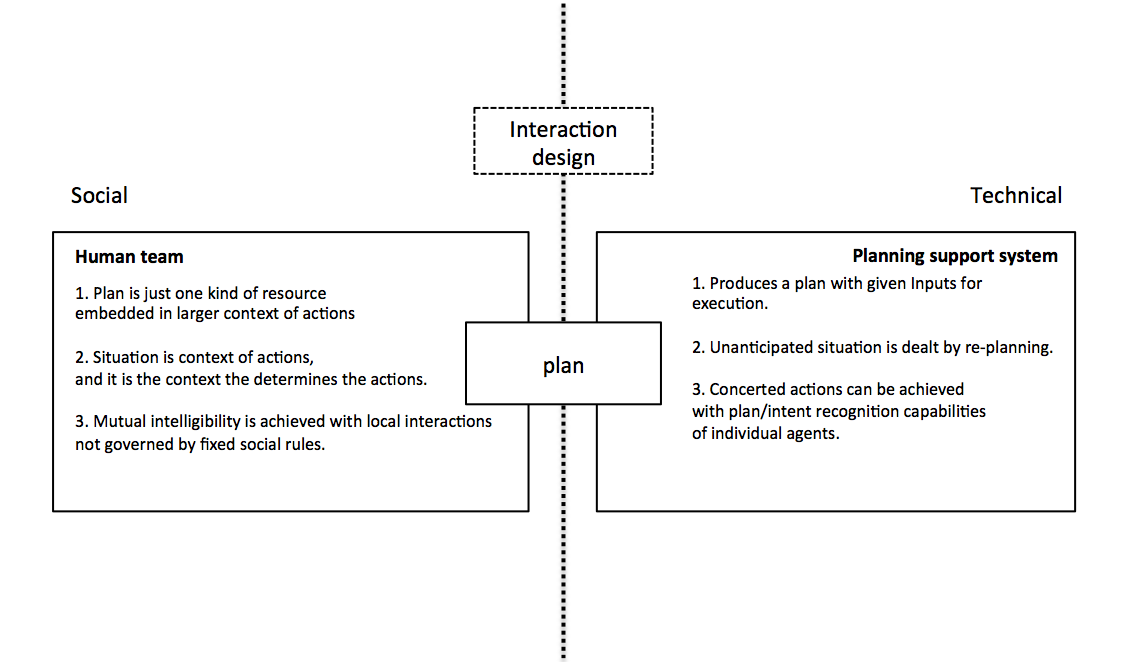
\includegraphics[width=1\textwidth]{img/approach/gap}
  \caption{ actions and situated actions}
  \label{fig:gap}
\end{figure}

%On the other hand, planning activities of responder teams are characterized by natural social processes such as communication, negotiation and cooperation. To support the responder teams with multi-agent coordination technologies, the confrontation between social and technical is inevitable. \\

% Situated action and purposful action.

%\ac{CSCW} Researchers have pointed out the existence of the inherent social technical gap - the great divide between what we know we must support socially and what we can support technically.  Some argued that human activity is highly flexible, nuanced, and contextualized and that computational entities and processes such as information sharing, roles, and social norms need to be similarly flexible, nuanced, and contextualized. However, current technology support systems for organisations are often rigid and inflexible, failing to fully support the social world. 

%Computer science is learning how to use techniques such as machine learning, user modelling to fill social-technical gap (section \ref{sec:LRHAI}). It is hard to disprove that a technical solution is imminent. However, some argued that such a technical solution is unlikely, given that computer science, \acf{AI}, information technology, and information science researchers have attempted to bridge the gap without success for at least 20 years \cite{Ackerman2000}.\\

%We argue that the social aspect does not need to be fully supported through technological advance. A deep understanding of social issues and appropriate interaction design may lead to possible ``workaround'' of the socio-technical gap. Although technology support may be not fully integrated with the social aspects, we believe appropriate interaction design can reduce its negative impact on social process so that the benefits of technology can overweight its adverse social impact. \\

%The field of HCI achieved widespread recognition with its inherent focus on the importance of the interaction between people and technology at the fundamental level rather than just the design of the user interface. It explicitly recognised the importance of the roles of the social and technical aspects of work. HCI Literatures have identified a wide range of different methodologies that helps inform the development of socio-technical systems such as (1) Cognitive Work Analysis, (2) Ethnographic workplace analysis, (3) Human-centred design. Some of the recognised HCI methodologies underpin the serious game approach employed by this PhD work to understand socio-technical design space of agent-based planning support. [The switch to HCI is not smooth]\\

%[Field trials supported by interaction analysis  speech act]\\

%[Andy s literature review of 2004 supporting ethnographic study should be cited]\\


\section{Serious Mixed Reality Game as a testbed} \label{sec:SMRG}
One of our work`s main objectives is to study interaction and coordination situated in rich and `messy' real-world socio-technical settings. As it is difficult to deploy technological prototypes in real disasters, a serious game approach has been adopted by researchers to study technology interaction in disaster scenarios through game-like simulations (Section \ref{sec:LRMRgame}).
%for example, to prepare first responders for scenarios in which hazardous materials are involved \cite{Losh2007}. \cite{Abbasi2012} also presented a study in which locally distributed participants played the role of victims asking for help via social media in a simulated crisis, and participants that played the role of first responders used a coordination system to filter messages and mobilize the appropriate responder teams according to their assigned capabilities.\\

This PhD work also adopts serious game approach to simulate a disaster response setting in which distributed responder teams coordinate under time and spatial constraints (Section \ref{sec:LRtaskplanning}). More specifically, we create a \acf{MRG} as a testbed that enables studying team coordination, interaction and communication in a real-world disaster scenario whilst providing confidence in the efficacy of behavioural observations (Section \ref{sec:LRMRgame}).\\

The \ac{MRG} testbed called \acf{AO} simulates a radioactive incident. Participants of the game play both the role of responders `on the ground', and coordinators in the control room. They coordinate with each other through GPS, map sharing and messaging, to achieve game objectives. The \ac{AO} game system can be integrated with planning agents to support players on the ground, and the interaction layer between players and agents can be configured in different ways through modifications to the game interface. Through agent integration and interface modifications, we created three `probes' of agent planning support with different interaction designs. The three probes are then be used to conduct behavioural studies, which allow us to unpack human system interaction with different interaction design patterns.\\

\section{The AtomicOrchid Platform}\label{sec:AOdescription}
We designed and implemented the mixed reality game \acf{AO} as a testbed for our field trials of different system interaction designs. The game involves field players on the ground (playing as field responders) and online players in a control room (playing as Headquarters (HQ)).

\begin{figure}[h]
  \centering
  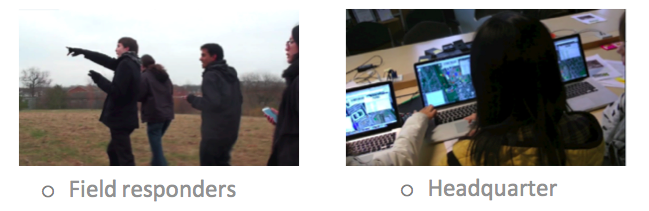
\includegraphics[width=1\textwidth]{img/approach/GameComponents}
  \caption{HQ and field players in AO}
  \label{fig:AOroles}
\end{figure}

In the following sections, we give a detailed description of the game design, which covers  grounding of the design rationale, the iterative design process, and the system architecture.

\subsection{Game mechanic} \label{sec:gameRatinale}
The AtomicOrchid is based on the fictitious scenario of a radioactive explosions creating expanding and moving radioactive clouds that pose a threat to responders on the ground (field responders), and the (virtual) targets to be rescued from around the game area. We chose a radiation scenario because unlike disasters that cause physical devastation it poses an invisible threat, which creates the need to monitor the environment closely with sensing devices, and communicate frequently.\\

Field responders are supported by a centrally located headquarters (HQ) control room, staffed by HQ players as coordinators who exchange messages with field players through an instant messaging style communication system. The messages are broadcasted, which means they are visible to all players. The core game mechanics are designed to allow us to explore specific aspects of team coordination. In particular, this is inspired by the real coordination challenge of resource and task allocation to coordinate spatially distributed resources and personnel. 

%The game`s two-tiered organisational structure is derived from real world disaster response organisation and from NIMS . The game`s HQ is loosely modelled on sector coordinators, whose role is to manage resources and communications between their assigned teams, and command and coordinate action within their sector (INSARAG, 2012). Field responders are modelled on team leaders and members. We ignore this distinction to simplify roles, assignments, and game mechanics.\\

%Whilst formal response teams tend to use radio to communicate (e.g., Toups et al., 2011) we chose text-based messages for its flexibility to support scenarios with many distributed (volunteer) field responders.\\

\textbf{Responder roles and targets}. Each field responder is assigned one of four roles:\\

\begin{figure}[h]
  \centering
  
\includegraphics[width=1\textwidth]{img/approach/AOroles}
  \caption{The roles in \ac{AO}}
  \label{fig:AOroles}
\end{figure}

There are also four types of (virtual) targets:\\

\begin{figure}[h]
  \centering
  
\includegraphics[width=1\textwidth]{img/approach/AOtargets}
  \caption{The targets in \ac{AO}}
  \label{fig:AOtargets}
\end{figure}

The objective of the field responders is to rescue as many targets as possible by `carrying' them to a drop off zone. To pick up and carry one of the target objects, two responders with particular appropriate roles must be in the proximity of the object. For example, a soldier and a transporter are required to pick up and carry fuel, and a medic and a soldier are required to pick up an animal (Figure \ref{fig:roleTargetMapping}).\\

\begin{figure}[h]
  \centering
  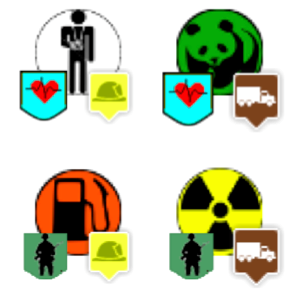
\includegraphics[width=0.3\textwidth]{img/approach/roleTargetMapping}
  \caption{Role target mapping}
  \label{fig:roleTargetMapping}
\end{figure}

The role-target mapping mechanic requires players to engage in resource coordination. Field responders have to engage in `agile teaming' forming, disbanding, relocating and re-forming in teams over the course of the game in order to complete the game objective. \\

\textbf{The radioactive cloud}. The cloud is a danger zone that can incapacitate field responders. It imposes spatial and temporal constraints on task performance and well- being. The cloud is analogous to various spatial phenomena in disasters (e.g. spreading fires, diseases and floods). It requires communication between HQ and field responders, as the spatial position and movement of the cloud is only known to HQ. The cloud is shown in a heatmap style in the figure \ref{fig:cloud}. The field player can detect `radioactive intensity' at their current locations with the mobile responder app.\\

\begin{figure}[h]
  \centering
  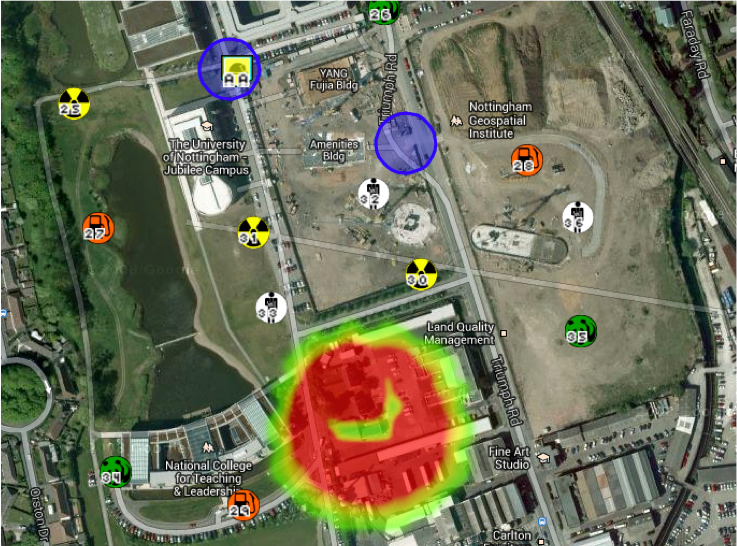
\includegraphics[width=0.8\textwidth]{img/approach/radioactiveCloud}
  \caption{The radioactive cloud}
  \label{fig:cloud}
\end{figure}

\textbf{Command-and-control (C2) structure}. The division of responsibility into HQ and field responders simulates a situation where  responders are connected to a generic two level \ac{C2} structure proposed by \cite{Chen2005}. This structure highlight the division between remote control room and on-site teams.  On-site responders react to immediate scene without global picture, while the coordination center deals with strategic issues and works with a global picture, leveraging external resources to help on-site response (\ref{sec:LRC2}). Instead of simulating a real command and control model such as \ac{BSG} (Section \ref{sec:lrstructure}), we chose the generic structure to simplify the game play, but still mirrors the main characteristics of \ac{C2} in \ac{DR}. \\

\textbf{System interface}. The system interface design is closely related to specific interaction designs, and it is refined evolving through three iterations of field trials. Therefore, the details of interface evolution are left to be introduced in the subsequent chapters (Chapters \ref{ch:studyone},\ref{ch:studytwo},\ref{ch:studythree}) describing field trials. \\



\subsection{System Architecture}
The AtomicOrchid system is based on the open-sourced geo-fencing game MapAttack(http://mapattack.org/) that has been iteratively developed for a responsive, (relatively) scalable experience. Our mixed-reality game relies especially on real-time data streaming between client and server. The client-server architecture is depicted in figure \ref{fig:sysArchitecture}. Client-side requests for less dynamic content use HTTP. Frequent events, such as location updates and radiation exposure, are streamed to clients using websockets to avoid the overhead of HTTP. In this way, field responders are kept informed in near real-time.\\

\begin{figure}[h]
  \centering
  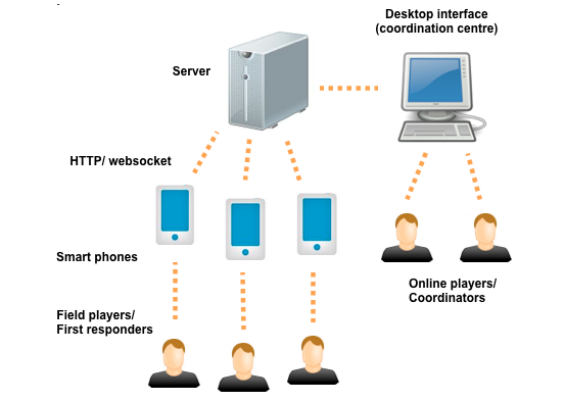
\includegraphics[width=1\textwidth]{img/approach/systemArchitecture}
  \caption{System Architecture}
  \label{fig:sysArchitecture}
\end{figure}

The platform is built using Sinatra for Ruby (http://www.sinatrarb.com/), and current web technologies such as socket.io, node.js, and AngularJs, and the Google Maps API. Open source mobile client apps exist for iPhone and Android; we adapted an Android app to build the Mobile Responder App.\\


\subsection{The planning agent}\label{sec:appagent}
In studies 2 and 3 (chapters \ref{ch:studytwo} and \ref{ch:studythree}), planning agents are integrated into the AtomicOrchid to support player's planning activities. The agents are developed by ORCHID Reseach partners from Southampton, more technical details of the planning agent is available in \cite{Ramchurn2015a}. In what follows, we briefly describe technical details of the agents and system integration between \ac{AO} and the agents.  \\

The coordination problem (described in section \ref{sec:gameRatinale}) is modelled using a Multi-Agent Markov Decision Process (MMDP) that captures the uncertainties of task execution, extending earlier work \cite{Wu2015}. The model allows responder actions to be delayed or to fail during the rescue process. The MMDP modelling leads to a large search space, even with a small problem. Hence,  an approximate solution is devised to save computation time, which can be executed to support real time planning. The planning algorithm takes into account both time (cloud and human movement speed) and spatial (path planning for responders) constraints. The planning algorithm run by the planning agent produces high quality task allocations that minimise the travelling distance of first responders, and maximise the number of targets rescued. Before the agent was deployed to support human teams in the game setting, computational simulations were used to benchmark MMDP algorithm against greedy and myopic methods (see figure \ref{tab:agentBenchmarking}). The results confirm that the algorithm produces efficient task allocations.\\


\begin{table}[h]
\centering
\begin{tabular}{c|lll}
Metrics               & MMDP  & myopic & greedy \\ \hline
\#completed task      & 71\%  & 65\%   & 41\%   \\
\#responders survived & 100\% & 25\%   & 0\%   
\end{tabular}
\caption{Result for MMDP, Myopic and Greedy algorithms, Credit \cite{Ramchurn2015a}}
\label{tab:agentBenchmarking}
\end{table}

For integration, the agent is deployed on a separate server. It communicate with the \ac{AO} game server through a pre-defined HTTP protocol (Appendix \ref{app:asprotocel}). The agent takes game status from the game server as input, which includes player's health, road connectivity, locations of players, targets and radioactive clouds. The output of the agent is a set of task assignments such as `player A and player B, go to target C' (Figure \ref{fig:inputoutput}) . The task assignments are sent to the \ac{AO} game server and presented to the game players. Detailed interaction design between human and the agent will be presented in Chapter \ref{ch:studytwo} and \ref{ch:studythree}. In order to facilitate the different interaction designs, the input of the agent is slightly different in study 2 and study 3, which will be detailed in sections \ref{sec:studyoneagent} and \ref{sec:studytwoagent}. \\

\begin{figure}[h]
  \centering
  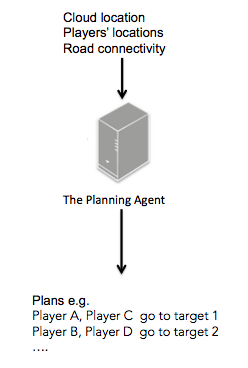
\includegraphics[width=0.5\textwidth]{img/approach/inputoutput}
  \caption{Input and output of the agents}
  \label{fig:inputoutput}
\end{figure}

\subsection{Logging system} \label{sec:applogging}
A logging system is also built into the AtomicOrchid system. The updates of game status sent between the game server and clients (both HQ and mobile clients) are all recorded in JSON format with system timestamps. The logs also contains the information of cloud status, task location and status (pick up/ drop off), messages, player location and health. Automated tools were also developed to reconstruct game play and visualise (Section \ref{sec:methdatahandling}) the log for data analysis. %The detailed log format is documented in Appendix x.

\subsection{Iterative design and development}
Before the game was deployed for observational studies in this PhD work, the game went through an iterative design and development process to test, refine game concepts and system robustness. We briefly describe three cycles of iterative game design and evaluation that took place before the system was ready for the first formal field study.\\

In the first iteration, we used a paper-based prototype to test and refine the core game mechanics. We recruited 12 participants, allocated one of four roles to them, and equipped them only with paper maps with locations of targets. They had to form different kinds of teams to retrieve the different kinds of boxes placed in the game area. The paper prototype demonstrated the demand for better support of situation awareness and communication to enable coordination. The technology prototype was first tested with users in the second iteration. Users were equipped with the responder smartphone app to communicate, navigate, locate and pick up targets in teams formed according to role requirements. HQ was staffed by members of the research team. A pilot study was conducted with members of the public that visited an Open Day at a local university. A total of 20 members of the public tested the game in four ad-hoc game trials. The lessons learned in the pilot study revealed problems with user interaction, networking, and game parameter tuning, which we subsequently addressed.\\

In the third iteration, we improved system stability and interface design. We conducted a pilot study at the campus of another university, to test the system in place. The full-fledged studies we report on later in this thesis was conducted shortly thereafter.\\


\section{Explore interaction designs with three AtomicOrchid studies}\label{sec:patterns} \label{sec:approachPatterns}

%[Justify the relation between the three iterations]
%- avoiding pitfalls that undermines observation of interaction arrangement
%- HQ agent interaction can be parallel/ HQ FR interaction follows progressive design interaction
%- The first iteraction: base case/ need to understand the organization before we do anything.\\

Based on the serious game approach, three studies are planned to explore the interactional issues related to the socio-technical integration of the planning agents and the responder team. To build such a socio-technical system, there are various ways to arrange the interaction between responder teams and a planning support agent. Inspired by the \acf{LoA} concept (Section\ref{sec:lrloa}) from research on automation design, we outlined 4 paradigms of human agent interaction loosely based on the automation level of planning activities: full manual, human in-the-loop, human on-the-loop, and Human-out-of-loop. This PhD work will only consider the former 3 notions of automation as explained before\\

In research of automation design, the \ac{LoA} model has been developed to categorise systems into a linear spectrum according to degree of automation. Arguably, the model may not fit perfectly into the context of socio-technical system due to some of its limitations identified in section \ref{sec:lrloa}. However, the terminologies that come with the model can still serve as a reference point for interaction designs to be studied in this PhD work.

%There are several variations of the LOA models. One example is the two-dimensional LOA model proposed by Parasuraman (detailed in literature review section x).Several limitations of the LOA has been identified in chapter x. Most importantly, the LOA model has a focus on one-to-one operator-system interaction (e.g. autopilots, tele-oportation). It fails to capture complexity of the interactions in the context of technology support for organisational work. Therefore, it does not fit into the context of socio-technical system, which is the main focus of this research. 

\begin{enumerate}
\item \textbf{Human out-of-the-loop}.
Out-of-the-loop represents the highest level of automation. An out-of-the-loop system is supposed to run completely independently. The human is replaced by the machine, therefore no human system interaction is required. This is unlikely to be realized in a socio-technical system, in which organisational work is mainly carried out by humans and supported by technologies.  \\

\item \textbf{Human on-the-loop}.
In this research we use the term Human On-the-loop to describe a system with high level of automation, which requires a minimum level of human intervention. Compared to out-of-the-loop, the on-the-loop system is designed to run without human intervention most of the times. However, human supervision and intervention are still required for contingencies. 

\item \textbf{Human in-the-loop}.
In this research human in-the-loop represents a system with medium level of automation. Compared to the On-the-loop system, the in-The-Loop system can not run without human input. Constant human interactions are required to achieve the goal of the socio-technical system. \\

\item \textbf{Full manual}.
A full manual system describes a system without automation. In the context AtomicOrchid, the platform without integration of the planning agent can be seen as a full manual system. 

\end{enumerate}

In the context of the AtomicOrchid platform, the notions of In-the-loop and On-the-loop can be used to describe the degree to which the planning agent automates the real-time task planning and the extent to which the human Headquarters need to be involved in the plan-execution loop. Guided by these 2 notions, we devised two detailed interaction designs for integrating the planning agent into the \ac{AO} game. In the next two sections, we give detailed description of the two interaction designs, followed up by an overview of the three field studies, which details how a sequence of system prototyping  and field trials was organised based on the two interaction designs, and how they are designed to serve the research objectives.\\

\subsection{The On-the-loop interaction}
The On-the-loop interaction is designed to facilitate the division of labour between humans and agent: a planning agent routinely assigns tasks to distributed responder teams, while human coordinators (the HQ) monitor and support the task execution by responding to arising contingencies (see figure \ref{fig:OnTheLoop}). In this design, the agent can directly contact field responders to allocate tasks. The responsibility of the planning agent is to generate and distribute plans for execution. The agent is also responsible for initiating re-planning according to changes in game status. The agent also directly handles feedback from the field player. i.e. the field players can give feedback to the agent by accepting or rejecting the plan, while the agent can generate new plans according to the feedback. \\

The role of the HQ is to monitor the planning process and provide support when contingencies arise. For example, the HQ may decide to stop some tasks issued by the agent if the threat of radiation increases unexpectedly. It should be noted that the agent can operate without HQ input, and the HQ intervention is supposed to be only occasional. \\

\begin{figure}[h]
  \centering
  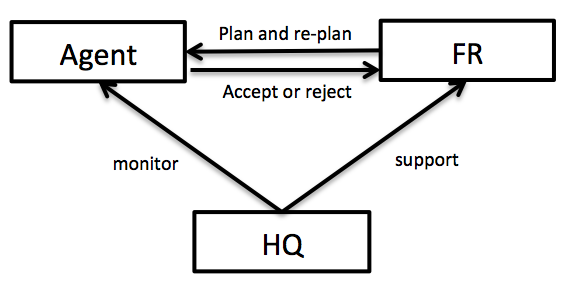
\includegraphics[width=0.5\textwidth]{img/approach/OnTheLoop}
  \caption{On-the-loop interaction design}
  \label{fig:OnTheLoop}
\end{figure}

\subsection{The In-the-loop interaction}
In-the-loop interaction is designed to facilitate a different pattern of labour division between humans and agent: a planning agent proposes the task assignments, and the human HQ needs to approve the tasks before they are sent to the field responders. In this design, the HQ can be seen as a mediator between field responder and the planning agent. If the HQ does not agree with a task allocations from agents, they can intervene by directly editing part of the plan or require the agent to re-plan. \\

Similarly, the feedback from the field responders (i.e. accept/reject) are delivered to HQ before any actions are taken. The HQ are responsible for reviewing the feedback and deciding what actions to take (e.g. decide to initiate re-plan, or ignore). Compared to On-the-loop interaction, the agent in this design will never directly communicate with field responders and the agent cannot operate without the HQ's input, i.e. the HQ have to make decisions on every agent proposed task, and take actions on the feedbacks from field responders. \\

\begin{figure}[h]
  \centering
  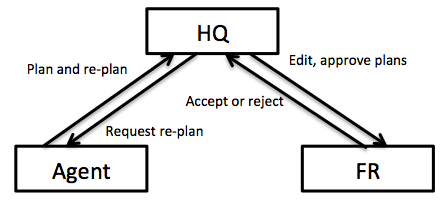
\includegraphics[width=0.5\textwidth]{img/approach/InTheLoop}
  \caption{In-the-loop interaction design}
  \label{fig:InTheLoop}
\end{figure}


\subsection{The three AO game studies}
Three studies are conducted to explore the socio-technical issues related human agent interaction. The first study focuses on a ``manual'' version of AtomicOrchid without agent support, while the latter two studies focus on On-the-loop and In-the-loop planning support respectively. For each study, we develop a \acf{MRG} to facilitate the interaction design to be studied. \\ 

The first study aims to observe and explore human coordination without planning agent support. The non-agent trial supports the two later (Chapter \ref{ch:studytwo}, \ref{ch:studythree}) agent-supported system trials by 1) revealing baseline performance of human coordination without agent support 2) and generating design requirements which feed into subsequent prototyping of AtomicOrchid. The purpose of the second and third studies is to investigate socio-technical issues related to the On-the-loop and In-the-loop interactions and derive design implications of interaction designs from the field observations.\\

\section{Collaboration with a Professional Disaster Response Organisation}
In addition to the three observational studies of AtomicOrchid games, a workshop with Rescue Global (a professional disaster response agency, see section \ref{sec:rg}) was organised to get professional feedbacks about the AtomicOrhid system and the planning support agent. Because the contact with Rescue Global was established at a late stage of this PhD work, the feedback from the \ac{RG} workshop are not used to drive the development of \ac{AO} game and interaction design, but to get an insight into the similarities and differences between \ac{AO} simulation and real world \ac{DR} operations, which help us to understand limitations and strengths of our observational study.  The \ac{RG} workshop happened between study two and study three (section \ref{sec:RGworkshopone}). The In-the-loop \ac{AO} probe was demonstrated to the \ac{RG} team and a discussion was organised to get feedback from \ac{RG}. It included a hands-on session for \ac{RG} members to experience \ac{AO} game, and further feedbacks was collected from discussions during and after the game session.\\

\subsection{Introduction of Rescue Global}\label{sec:rg}
\acf{RG} is a disaster response organisation. They are a UK charity and a US not-for-profit headquartered in London, UK. Their remit is to provide ``immediate crisis and disaster reconnaissance ability, delivering accurate and timely information and risk data, as well as performing emergency search and rescue operations where needed to save life.'' One example of their operation is the deployment of a reconnaissance team in the Philippines for super typhoon Haiyan in 2013. After the typhoon strike, the team conducted disaster reconnaissance on isolated islands from the air and on the ground, assessing needs and delivering aid based on priorities of water, food, medicine and shelter.\\

\ac{RG}`s organisational structure represents a typical hierarchy found in emergency services \cite{U.S.DepartmentofHomelandSecurity2008}, termed Gold, Silver and Bronze. Gold denotes the strategic lead, which is associated with \ac{RG}`s senior officers (often referred to as the `head shed') and the headquarters in London, Silver is the tactical lead, which is `spun up' for mission planning, both to assess feasibility of deployments and when actually deployed on-site. Bronze refers to the operational level, in which `Pathfinders' (field responders) carry out operations `on the ground' supported by Silver command \cite{RescueGlobal2012}. \ac{RG}`s core staff consists of around 20 highly specialised experts and admin support, many of whom have had prior careers in the military, emergency and first response services.\\

%\section{A framework of interactional issues}\label{sec:interactional}
%interaction techniques 
%[Which Interaction Technique Works When] refer to interaction techniques may refer to is a set of %interface widget design.

%We follows a process of interaction design documented in the [Designing interactions p 15], the process %is interactive, with a special focus on understanding issues and generating design implications . The %issues emerges in previous iterations will be feedback to next iterations. 

%interactional issues: 

%Interface aspects: tech dependent or not?
%interaction aspects: concerned with interaction patterns 
%Social aspects: Corncerned with what? 

%(Sedig, K.Parsons, P) pattern based approach.
%(Most interaction techniques literature reviewed so far is about study in visual representation. )
%(Interaction design, wiki)

\chapter{Methodology to Investigate Human Agent Interaction}\label{ch:methodology}
This chapter takes an in-depth look at the methodology that underlies the empirical approach adopted in the presented studies.This PhD is based on ethnographic-oriented field studies based on the \acf{AO} platform to generate descriptive results, which contains rich interactions among participants and the planning support system. Ethnographic observations and interaction analysis are central to all three field studies, while group interviews, message classification, and system log analysis supplement the two former in-situ methods.\\

\section{Ethnomethodological perspective}
Observation of participants in the field study is informed by \acf{EM}. Following the tradition of ethnography, \ac{EM} seeks to explicate the real-world organisation of work by adopting a naturalistic stance. \ac{EM} places methodological emphasis on rigorous description of the situated (i.e. local, observable) actions and practices \cite{Suchman1987} in and through the contingent accomplishment of daily activities. \ac{EM}-informed ethnography arguably helps to answer what might be regarded as an essential question in design: what to automate and what to leave to human skill, competence, judgement, experience and expertise \cite{Crabtree2012}. By producing description of the actions and practices in and through which the work `gets done' time and time again by the members, \ac{EM} can inform system design by uncovering what actions and activities we should therefore support.\\

For the purpose of this thesis, the social situation of the interaction with and around the planning support is argued to be a critical factor to understand how the social organisation of work is achieved. Observation of the situated actions and practice employed by the participants was a key method for the field study. The use of the system was observed and filmed for later analysis. Video is widely recognised as an important resource for ethnography around technology use \cite{Crabtree2012}. The next section goes through the method of video-based interaction analysis for unpacking the interactions observed in the field. \\

\section{Interaction Analysis} \label{sec:aprIA}
Interaction analysis can be defined as an interdisciplinary method for empirical investigation of interaction of human beings with each other and with objects in their environments \cite{Jordan1995}. In the context of \ac{HCI} study, it is a method of analysing naturally occurring talk and activity, with the aim of uncovering and describing something of the order and organisation by which people interpret and interact with each other and with the things around them.\\

The advantage of interaction analysis lies in its ability to deal with actual details of technologically mediated interactions and allows technology developers to see exactly how technology fits (or doesn't fit) into current working practice. Other methods such as questionnaires and interviews rely upon reports from participants, rather than actual, reasoning and behaviour. The over-reliance on participants' report make those methods vulnerable to the problems of people producing post-hoc rationalisations of actions, forgetting or incorrectly estimating aspects of behaviour, expressing ineffective attitudes, and generally lacking insight into the tacit procedures underlying much of their activity. Instead, interaction analysis can expose the practical reasoning activities of participant's themselves in a way which does not require them having to remember, justify or even know what they did. This effectively indicates how people think and make sense of technology they are using, in the performance of some task. However, interaction analysis is extremely time-consuming, which means it can only be carried out on small numbers of participants. This limitation makes it unsuitable for answering to very specific design questions and for examining the needs and behaviours of diverse groups of people. Further, the generality of its findings may need to be established by other means \cite{Jordan1995}.\\

For the purpose of this PhD work, interaction analysis is applied to evaluate the game probes undergoing field trials in the work settings of Disaster Response. In this case, the description generated by interaction analysis could expose information on the sequential organisation of technologically and socially mediated activities, which in turn, reveals how the activities can be supported. The main resource of interaction analysis is video recordings of \ac{AO} game plays. The video analysis generally consists of three stages \cite{Heath2010} :

\begin{enumerate}

\item Cataloguing the data corpus. This step involves a preliminary review of the corpus. Basic aspects of the activities and events are catalogued at this stage. Preliminary reviews and cataloguing should involve no more than a simple description and classification of the materials without detailed analysis. \\

\item Selecting Episodes. In light of preliminary review of data, a more focused substantive review of data is carried out in this stage. Repeated analytical searches of the data corpus are also involved to find examples of actions that appear to reflect similar characteristics. Candidate episodes of the particular phenomena, actions or organisation under scrutiny should be gathered and put into collections. \\

\item Detailed analysis.  We begin to look more closely at the selected candidate episodes to unpack the way in which interaction is accomplished by participants. The process generally involves transcribing and analysing both talk and visible conduct in the candidate episodes. \\ 

\end{enumerate}

In later chapters, results of interaction analysis are presented by detailed episodes of game play. In those episodes, a standard orthographic notation is used, \cite{Jordan1995} and complemented by timestamps [0:00], and system messages from remote players and HQ. Players can be uniquely identified by their initials. Targets are denoted by their unique numeric target id. Task assignments from the planner support system are represented as two initials and one target id connected by a rightward arrow. For example, the notation PC, CR -> 22 means player PC and CR are instructed to team up and go for target 22.\\




\section{Data collection and handling}\label{sec:methdatahandling}
Interaction analysis has been introduced as the main method for investigating socio-technical issues in our studies. This section introduces a number of methods employed for data collection and handling. In particular, the group interview supplements field observation by providing subjective description of game play experience. The message classification method gives an quantitative overview of remote communication. It also provides context for interactions in the field and helps to identify interesting game events. The system log analysis produces game event visualisations and replay. When triangulated with the video data, the log data analysis also supports interaction analysis by providing context and helping to identify interesting episodes in videos.\\

\subsection{Video and audio recording}
Audio recorders and video cameras are believed to valuable resources for ethnographic study. Both audio and video recordings offer us a rich resource and enable us to elucidate the methodical ways in which work is organised and accomplished as an interactional matter \cite{Crabtree2012}. This PhD work uses video/audio recordings to capture distributed activities in the \acf{AO} game as it happens, and the subsequent interaction analysis is based on reviewing the video recordings. \\

For each \ac{AO} studies, multiple researchers were hired to capture activities of distributed teams in the field. The researchers were instructed to follow player teams and film their actions including talking, gestures, and other bodily activities. In some cases, there weren't enough researchers to cover all the player teams in the field. To maximise the number of teams covered, the researchers were instructed to avoid filming the same player teams at the same time. In the control room, one researcher recorded the actions of Headquarters players with two camcorders. One camcorder was fixed on a tripod and the other was held by the researcher. \\

Audio recordings were used to supplement videos. An audio recording app was installed in the Android phones that were used by the field players in the \ac{AO} game. The app works in the background, recording player's voices without interrupting players' use of the AtomicOrchid client app. The obvious limitation of audio is that we cannot visually see player's actions with it, while its strength lies in its guaranteed coverage of all player teams at all times. As a great deal of the work of a setting is conducted through talk \cite{Crabtree2012}, audio recordings are useful alternative resources for interaction analysis when video coverage is not sufficient. \\


\subsection{Log Data Handling} \label{sec:aprloghandling}
Nowdays, \acf{HCI} researchers often collect rich dataset for investigating interactions. The data set becomes larger and larger as digital record systems increase in availability \cite{Brundell}. Automated tools are increasingly necessary for managing the organisation, replaying, structured and free coding (and annotation) and analysis of these growing data sets \cite{Brundell}. For this research, the logging system of AtomicOrhid produces time-stamped system logs. The raw log data is hard to be use directly as a resource for interaction analysis. In order to reveal the information buried in the logs, the data has to be processed so that it can be easily read and triangulated with data in other modalities i.e.  video and audio recordings. There are a number of tools already in existence to automate data handling and support the analysis of interactions. However, these tools often have limited or very specific functionalities \cite{Brundell}. Therefore, we developed our own data visualisation and log replay system which are tailored to handle the raw log data from AtomicOrchid studies.\\

To recap (Section \ref{sec:applogging}), the logging system records players's location, health, targets' location and status (pick up/drop off), task assignments and players' feedback (reject/accept). The data visualisation tool (Figure \ref{fig:logvis}) focus on visualising task assignments in the game play. The game events related to task allocations, including task assignments, player feedback, target pickup and dropoff, are all plotted on a time line with different annotations. The colored dots and squares denote various game events (Figure \ref{fig:logvis}). Detailed information of the event can be displayed when mouse hover on. As can be seen in Figure \ref{fig:logvis}, the deep blue dot with mouse cursor hover on denotes a target pick up event. The two players with initials CY and DS (see lines connecting the pick-up events) picked up target 598 at the 10th minute of game play. This data visualisation tools give an overview of the game-event sequence. It assists interaction analysis by providing context and guidance in the episode selection process. \\

\begin{figure}[h]
  \centering
  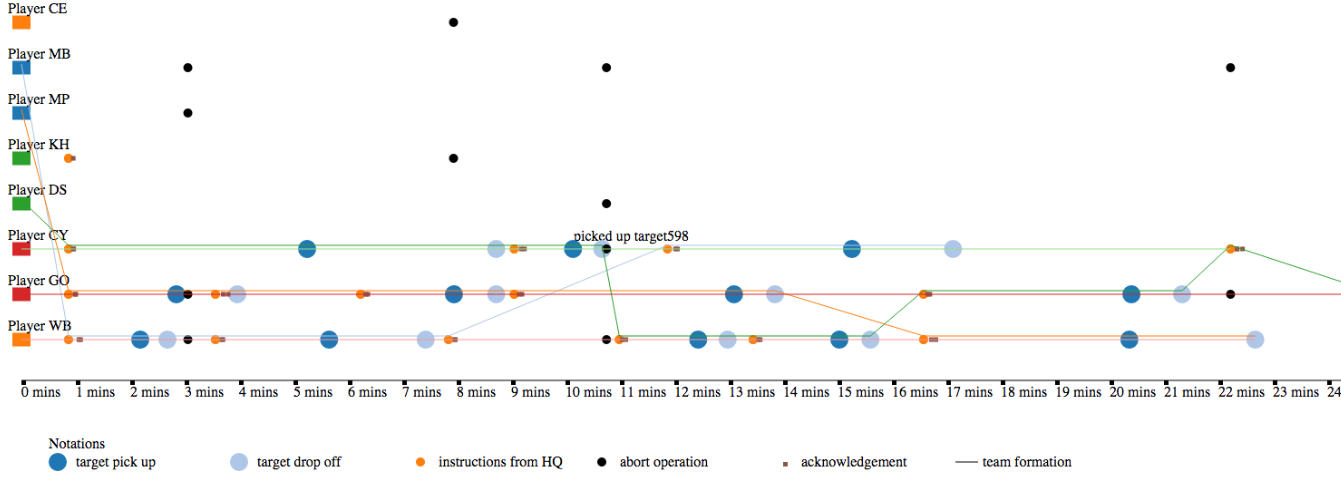
\includegraphics[width=1\textwidth]{img/methodology/logVisualisation}
  \caption{Log visualisation}
  \label{fig:logvis}
\end{figure}

A replay system was also built to triangulate multiple videos with log data. The main map view on the replay interface (Figure \ref{fig:replay}) displays game status reconstructed from log data, in a way that is similar to the HQ interface does. By giving a time offset to each video file, the videos are synchronised with the main map view of game status. The replay system is an important tool for interaction analysis, as it presents distributed game play with a single interface in a synchronised way, providing insights into the distributed interaction among participants and the system as it happened in parallel. \\

\begin{figure}[H]
  \centering
 \rotatebox{90}{
  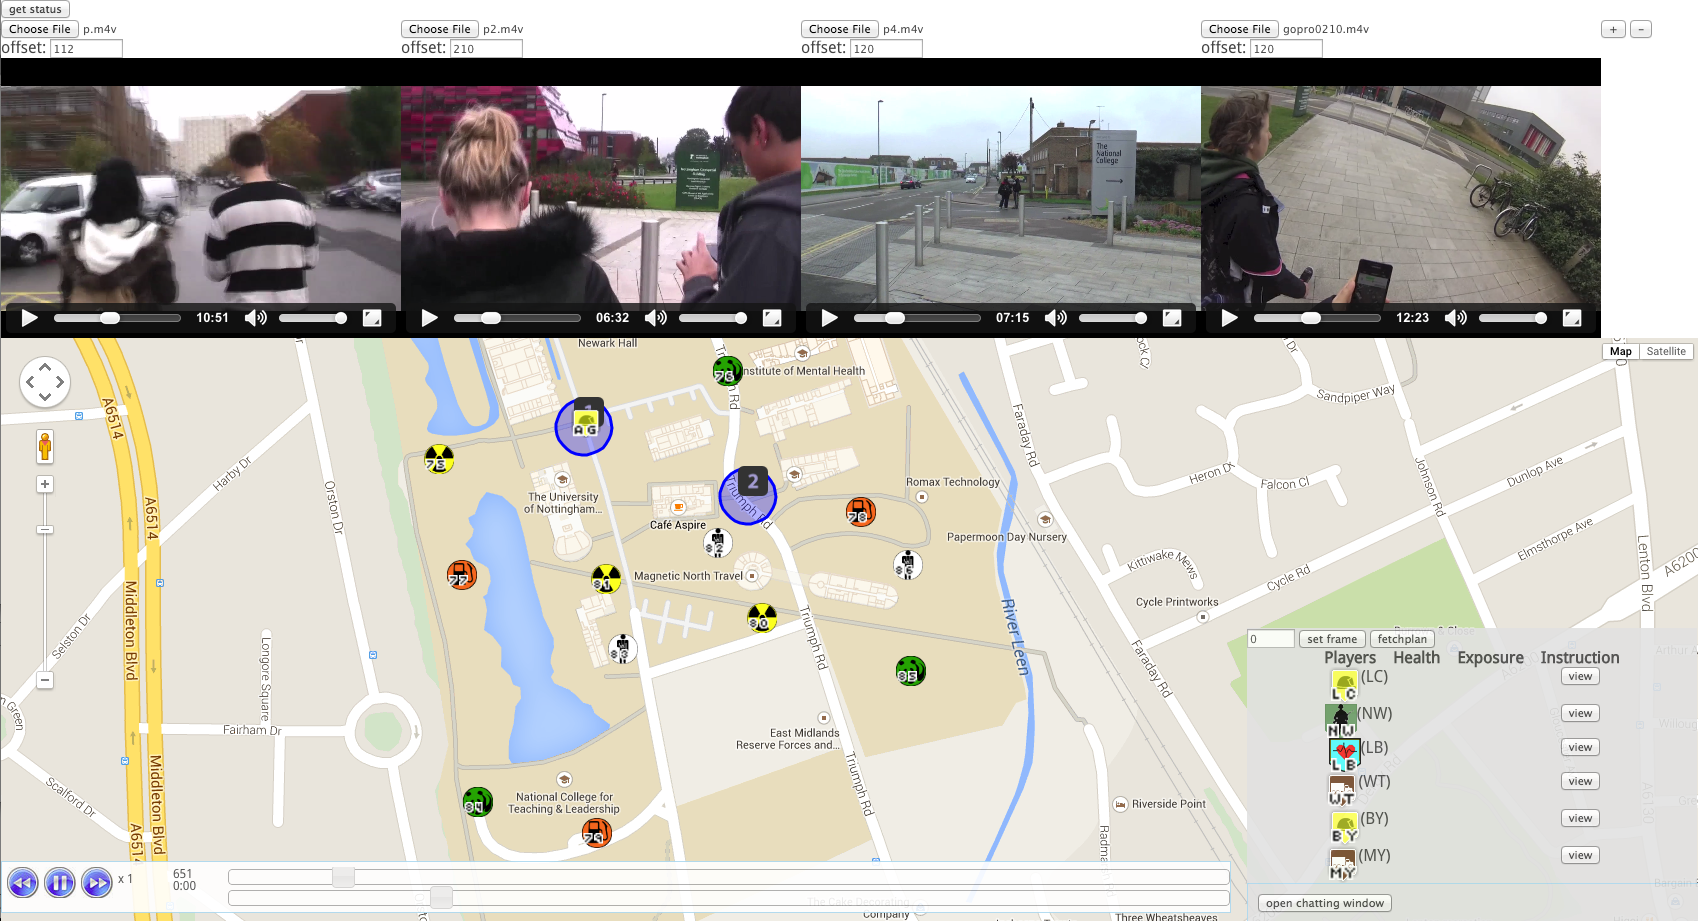
\includegraphics[width=1.5\textwidth]{img/methodology/replay}
 }
  
   \caption{Replay system}
  \label{fig:replay}
\end{figure}
\newpage
\subsection{Message classification} \label{sec:aprmsg}
In AtomicOrchid, remote coordination between field and human HQ is achieved through a text messaging channel. The remote messages are recorded as part of system logs. To understand how the team members interact through the remote messages, we devised a message classification method based on speech act theory \cite{Searle1976}. We used speech-act theory and the notion of adjacency pairs \cite{Avrahami} to classify messages sent between and among responders and HQ. According to speech act theory, utterances in dialogues can be considered as speech acts from three dimensions \cite{Searle1976}. We were primarily concerned with the illocutionary dimension of speech acts.\\

Searle`s classification of illocutionary acts is used to categorize messages in the communication system as follows.\\

\begin{enumerate}
\item Assertives: speech acts that commit a speaker to the truth of the expressed proposition.
\item Directives: speech acts that are meant to cause the hearer to take a particular action, e.g. requests, commands and advice.
\item Commissives: speech acts that commit a speaker to some future action, e.g. promises and oaths.
\item Expressives: speech acts that express the speaker's attitudes and emotions towards the proposition, e.g. congratulations, apologies and thanks.
\item Declarations: speech acts that change the reality in accord with the proposition of the declaration, e.g. pronouncing someone guilty.
\end{enumerate}

The notion of request-response adjacency pairs are also used to gain insights into the reciprocity of communication. In linguistics, adjacency pairs describe conversational turn taking \cite{Avrahami}. In AtomicOrchid, we expected many actions in remote conversation to be accomplished through pairs of utterances such as request-response, question-answer, or inform-acknowledge. For simplicity, we ignore the typology of adjacency pairs and treat all pairs as request-> response. Any utterance that expects a response is considered as a request.\\

The purpose of this message classification is to give an overview of the communication in the message channel. Meanwhile, the results of message classification supports interaction analysis, as it helps to identify interesting moments of team interaction in the game such as important decision points.\\

\subsection{Group interview}
For all three field studies, group interviews were conducted with all participants after each game sessions. The interviews consist of open-ended questions with the aim to supplement the field observation and interaction analysis with participants' comments about their experiences of the game. The interview is `informal and unstructured' in the sense that it is not driven by pre-defined questions, but only by the research scope and interest. It is conducted in the manner of a conversation taking place between the researcher and the participants \cite{Crabtree2012}. The interview does not stand on its own to provide distinctive results. The primary aim of the interview is to develop an overview of participants' experience of the game. Meanwhile, emergence of unanticipated issues and events was also fostered by asking open-ended questions, which in turn, are used to establish context for the issues for interaction analysis.\\

\section{Analytic Procedure}
To sum up, interaction analysis is the main in situ methods applied in the studies. The data collection and handling processes are supported by methods including log data handling, group interviews and message classification. With this inventory of research methods, we can depict a typical analytic procedure for analysing the interactions in as AtomicOrchid study. \\

The procedure (Figure \ref{fig:analyticprocedure}) begins with field studies after which a set of data are collected from three sources including system logs (1.1), video/audio recording (1.2) and group interviews (1.3). The message logs are then classified according to speech act theory. The resulting classification gives quantitative insight into the remote communication. The further log data handling produces replay and visualisation of game events. \\

The output of data handling process are then used as resources for interaction analysis. The message classification (2.1) contribute to catalogue building process (3.1) in the interaction analysis by augmenting the context of remote communication. The data visualisation (2.2) also helps to identify important episodes of interaction and provide context for further episode analysis. The game replay (2.2) triangulate video recordings with system logs. It is used as the major tool for in-depth data examination in the episode selection and analysis process (3.2,3.3), as it provides synchronised view of multiple videos and system logs. Additionally, the players' comments from the group interview give us insights into participants' subjective game experience, which are also important context for episode analysis.\\



\begin{figure}[h]
  \centering
  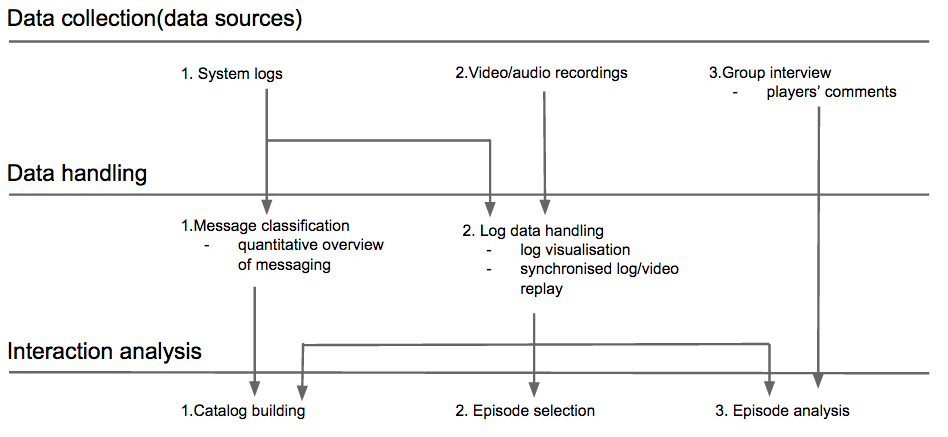
\includegraphics[width=1\textwidth]{img/methodology/analyticprocedure}
  \caption{Analytic procedure}
  \label{fig:analyticprocedure}
\end{figure}


%\addtocontents{toc}{\protect\clearpage} % <--- just debug stuff, ignore
\part{Studies}
%************************************************
\chapter{AtomicOrchid Study 1: Non agent version}\label{ch:studyone} % $\mathbb{ZNR}$
%************************************************
In this study, we analyse team interactions in an \acf{AO} game setting which simulates a time-critical distributed task environment in a disaster response operation. This study uses the full manual version of \acf{AO} without automated planning support. Players are provided with basic coordination support including remote text messaging, GPS/map sharing. Interaction analysis is conducted to examine log data and field observations revealing local and remote coordination within the responder team. We generate design implications for automated planning support and uncover requirements that highlight the role of local coordination, decision-making resources, geo-spatial referencing and message handling. \\

\section{Introduction}
%\acf{DR} has been characterised as highly coordinated, time-critical collaborative activities  \cite{Mendonca2007}. Coordination is essential in such settings so that time critical interdependent activities such as search and rescue can be completed in a timely and satisfactory manner \cite{Bradshaw2011}. Opportunity space for building `intelligent' task planning support for  such activities has been recognised by the researchers of \ac{HACS} systems (Section \ref{sec:lraisupport}). However, little study has explored the design space for \ac{HACS} systems to support time-critical coordination settings. Therefore, little is known about the challenges and requirements in building systems to support planning for responder teams in such settings.\\

%Due to the critical nature of the disaster operations, it is hard to design and deploy `intelligent' task planning support in the field before we thoroughly explored the requirements of interaction design. On the other hand, computational simulation of an `intelligent' system is fundamentally insufficient for studying socio-technical issues (Section \ref{sec:sociotech}). 

In this study, we aim to use the version of AtomicOrchid game as a research probe to uncover the requirements and design implication for building `intelligent' coordination support system. The AtomicOrchid game creates a socio-technical setting in which player teams plan and executes spatially distributed tasks (see section \ref{sec:sociotech}). Although \ac{AI} researchers has envisioned that an intelligent agent can support task planning by providing computational optimised task allocations in real-time, we focus on a manual version of AtomicOrchid which does not involve any computational planning support. The primary objective is to unpack how human teams coordinate in the time and space constrained task setting through interaction analysis of behavioural data collected from field trials. In particular, the interaction analysis focuses on two aspects of coordination in \ac{AO}, namely `remote' and `local'. The remote aspect is concerned about the coordination activities across distributed teams and remote HQ, which are typically mediated by computational systems. The local aspects is about coordination within co-located teams, in which face-to-face conversations plays a major role. Drawing on the results of the interaction analysis, we aim to generate design requirements and implications for automated planning support. \\

Additionally, this study also supports our later system development and trials. As the first of three iterative trials in this PhD work, this non-agent trial supports the two later Chapters \ref{ch:studytwo} and \ref{ch:studythree} agent-integrated trials by (1) revealing baseline performance of human coordination without agent support (2) generating design requirements which feed into subsequent refinement of AtomicOrchid. The requirements are critical in that (1) the later studies can use them to recognize non-agent related design factors and (2) it also can inspire the interaction design between agent and responders in later system refinement.  \\

%rephrase
%Findings from the study highlight the social processes in which players organise their coordination tasks locally and remotely. We discuss the division of labour between humans and teams; the interactional problems emerged from the remote coordination. We conclude the paper with a number of emerging interaction design requirements to consider when building planning support systems for human teams, which emphasises on system support for remote coordination. \\

In what follows, we expand on the description of the \ac{AO} system in chapter \ref{ch:approach} with a focus on interfaces and interaction design that are specific to this study. We then present results of the interaction analysis, followed by a discussion of performance implications derived from the results, before we move to design requirements. \\

\section{System Description}\label{sec:study3system}
% ===== how do I split this with Approach chapter
The basic game mechanic and system architecture have been introduced in the chapter \ref{ch:approach}. This section gives a detailed description of the system interface that support coordination between the field responder(FR) and headquarter(HQ) players. \\

% the HQ interface 
In this, study, HQ is manned by 2-3 coordinators. All of the coordinators are provided with a web-based coordination interface (Figure \ref{fig:HQinterface}). The interface gives them an overview of the game status and enable them to communicate with the field responders. \\

% insert image here.
\begin{figure}[h]
  \centering
  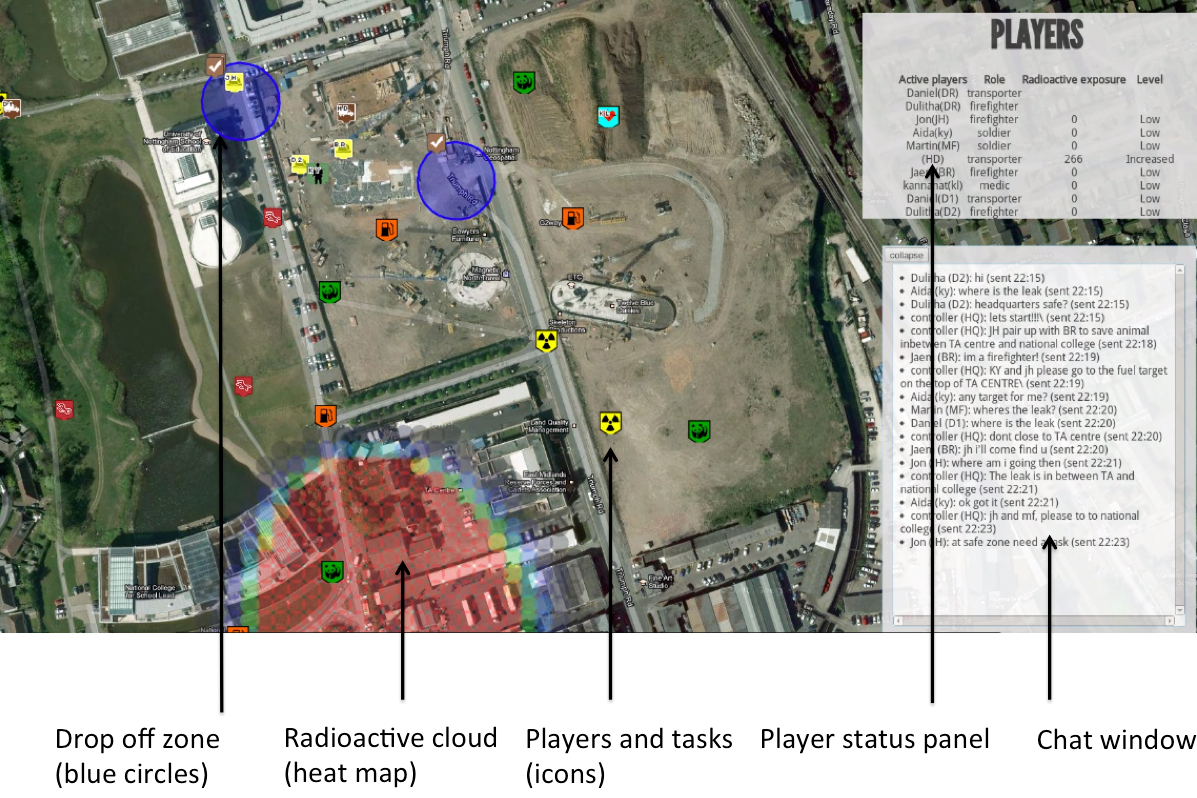
\includegraphics[width=1\textwidth]{img/study1/webinterface}
  \caption{The HQ interface}
  \label{fig:HQinterface}
\end{figure}

As can be seen in the figure \ref{fig:HQinterface}, the majority of the interface is occupied by a map-based presentation of the game status. Roles and locations of field responders are represented on the map as icons. The field responders can be uniquely identified by their initials shown on the icons. The target types and locations are also shown as icons on the map. Location and intensity of radioactivity is indicated by a heatmap. Health status (health value ranges from 0 to 100) of the field responders is displayed on the right-top panel. A chatbox is placed at the right bottom for HQ to browse and send messages. The messaging system follows a broadcasting model. Everyone can send messages to one public channel, and the messages are visible to every player through the mobile and HQ interface.\\

Field responders are equipped with a mobile responder app providing them with sensing and awareness capabilities (Figure \ref{fig:mobileResponderApp}). There are two tabs in the responder app. The ``map'' tab displays a map showing locations of field responders and targets, which is similar to the map on the HQ interface, except that the radioactvity is not shown. The radiation level of the players` current location is displayed as a Geiger counter reading (shown as a number on the top left of the screen), which ranges from 0 to 100. Health status of the field responder is indicated by a health bar on the right side of the Geiger counter. The chatbox (similar to the one on HQ interface) is placed on the "Messages" tab for the field player to receive and send messages.\\

% the mobile responder app
\begin{figure}[h]
  \centering
  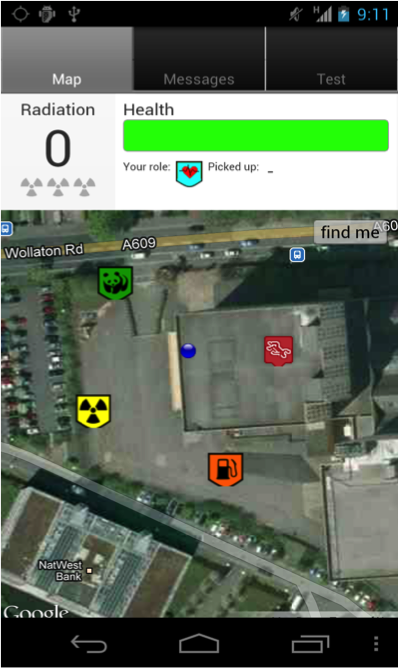
\includegraphics[width=0.5\textwidth]{img/study1/mobileinterface}
  \caption{The mobile responder app}
  \label{fig:mobileResponderApp}
\end{figure}

% move this to the study 1 chapter. 
 %The app shows a reading of radioactivity, their health level based on radioactive exposure, and a GPS-enabled map of the game area with the targets to be collected and the drop off zones for the targets. Icons according to responder roles that additionally have their initials on them can be used to identify individuals. Another tab reveals the messaging widget to broadcast messages to the other field responders, and to headquarters.\\

\section{Study Design}\label{sec:study1procedure}
% ====== checked from COOP, should be fine =======
We ran two AtomicOrchid Game sessions. We describe participants, procedure, session configuration, and methods used to collect and analyse quantitative and qualitative data.\\

Study participants were recruited through posters and emails. A total of 18 participants were recruited; 7 participated in session A and 11 in session B. All participants were reimbursed with 15 pounds for 1.5 hours of study. In session 1, there was 2 HQ player and 5 field players. In session B, there were 8 field players and 3 HQ players. The session A have fewer participants then session  B because fewer participants turned up in the study of session A. Although participants are fewer than expected, we still believe that session A can provide valid observation of organisational conducts in \ac{AO} setting.\\

The majority of participants were students of the local university (Appendix \ref{app:demo1}). Upon arrival in the HQ (set up in a meeting room at the local university), participants were briefed and asked to consent to participate. Roles were randomly assigned to all participants (HQ/field responders: firefighter, medic, transporter, soldier). Field responders were provided with a smartphone; HQ coordinators with a laptop. Game rules and interfaces were introduced, and participants were assisted in setting up their phones and laptop clients. Field responders and HQ coordinators were given 5 minutes to discuss a common game strategy. All field responders were accompanied to the starting point within the designated game area, about 1 minute walk from headquarters.\\

Once field responders were ready to start, HQ sent a ``game start'' message. Gameplay commenced for 30 minutes. A ``Game over'' message by HQ concluded the game. Field responders returned to HQ for the post-game session. A group interview was then conducted, before participants were debriefed and dismissed.\\

The size of the game area on the local university campus is 400 by 400 meters, without heavy traffic (Appendix \ref{app:area1}). The terrain of the game area includes grassland, a lake, buildings, roads, and footpaths and lawns. There are two drop off zones and 16 targets. The pilot study showed that this was a challenging, yet not overwhelming number of targets to collect in a 30 min game session. There were four targets for each of the four target types. The pattern of cloud movement and expansion was the same for both game sessions.\\

As described in chapter \ref{ch:approach}, we took a mixed methods approach to data collection and analysis. Five researchers with camcorders recorded the game play. One researcher recorded action in the HQ, and four other researchers each recorded a field responder team. In addition to video recordings, a semi-structured group interview was conducted aiming at eliciting important decision points, strategies and the overall decision-making process. Time stamped system logs were collected that contained a complete record of the game play, including responders` GPS location, their health status and radioactive exposure, messages, cloud location, locations of target objects and task status. \\

\textbf{Data handling} Firstly, the log data (including remote messages) are handled by a digital replay system to reconstruct the game state (Appendix \ref{app:vis1}) that can be triangulated with video data to support interaction analysis (Section \ref{sec:aprloghandling}). Secondly, to give an overview of how remote messages are used as a coordination resource, we used speech-act theory and the notion of adjacency pairs in linguistics to classify messages sent between and among responders and HQ (Section \ref{sec:aprmsg}).\\

\textbf{Interaction analysis} We focus on the analysis of local field responders` interaction to unpack team coordination, including handling of messages sent by HQ. Video recordings of field action were catalogued to identify sequences (episodes) of interest (\ref{sec:aprloghandling}). Key decision points in teaming and task allocation served to index the episodes. Interesting distinct units of interaction were transcribed and triangulated with log files of relevant game activity for deeper analysis that we present in this chapter. Results of interaction analysis will be presented by detailed episodes of game play, with standard orthographic notations introduced in section \ref{sec:aprIA}. \\

\section{Data analysis and results}
Here, we present findings from interaction analysis supported by message classification that reveal how team coordination was achieved. Overall, responders rescued 7 and 9 targets in sessionS A and B, respectively, out of 16 targets in total per session (Table \ref{tab:gameResults1}). Two players were incapacitated in session A, and 1 player was incapacitated in session B. 117 and 70 messages were sent in sessionS A and B, respectively.\\

\begin{table}[h]
\footnotesize
\begin{tabular}{llll}
\multicolumn{1}{l|}{} & Saved targets & Incapacitated players & Remote messages \\ \hline
\multicolumn{1}{l|}{Session A} & 7 (out of 16) & 2                    & 117             \\ 
\multicolumn{1}{l|}{Session B} & 9 (out of 16) & 1                    & 70              \\ 
\end{tabular}
\caption{Overview of game results}
\label{tab:gameResults1}
\end{table}


In what follows, results of the message classification will be presented first, followed by detailed analysis of episodes.\\

% this is from COOP paper, need to adapt it for this writing 
%{An overview shows that directives from HQ are frequently not brought up locally. A further episode demonstrates how field responders instead draw on technological and embodied resources to achieve local coordination, without HQ involve- ment. Finally, two more examples illustrate how responders routinely employ messages as a resource to support situational awareness.\\ %}

\subsection{Results of message classification}
We used Searle`s classification (Section \ref{sec:aprmsg}) of speech acts to categorize messages (Table \ref{tab:speechact}). The table \ref{tab:speechact} shows that the majority of massages are directives and assertives sent by HQ. The majority of messages from field responders are requests for information, team and tasks. In what follows, we present examples for each category of speech acts, which in turn, provide an overview of remote coordination that is supported by the remote messaging system. \\

\begin{table}[h]
\footnotesize
\begin{tabular}{lllllp{5cm}l}
Speech acts  & \multicolumn{2}{l}{Session A} & \multicolumn{2}{l}{Session B} & \multicolumn{1}{c}{Example} & Total    \\ \hline
             & HQ            & FR            & HQ            & FR            &                                                                            &          \\ \hline
Directives   & 57            & 0             & 32            & 0             & JH pair p with BR to save animal in between TA centre and national college & 89(47)\% \\
Assertives   & 25            & 2             & 8             & 4             &                                                                        The leak around geospatial is bigger & 39(20)\% \\
Expressives  & 5             & 0             & 0             & 0             &                                                                           Good Job, JJ, TV and RL & 5(2\%)   \\
Declarations & 3             & 0             & 0             & 0             &                                                                           NOTICE - TEAM B: NS + TD & 3(1.6\%) \\
Commissives  & 0             & 4             & 0             & 4             &                                                                           ok got it & 8(4\%)   \\
Requests     & 8             & 6             & 0             & 19            &                                                                           wheres the leak? & 34(18\%) \\
Unclassified & \multicolumn{2}{c}{7}         & \multicolumn{2}{c}{2}         &                                                                            & 9(5\%)  
\end{tabular}
\caption{Speech act classification}
\label{tab:speechact}
\end{table}

\subsubsection{Directives}

Most messages in the category of directives are instructions sent by headquarter (HQ) players. The content of instructions can be related to two themes: task allocation and task execution. The purpose of task allocation instructions is to distribute plans to field teams and require them to execute it. Most instructions in this category follow a common pattern. Taking the following message as example:\\

\begin{quote}
\texttt{``HQ : JH1 pair up with BR to save animal inbetwen TA centre and national college''}\\
\end{quote}

The instruction sent from HQ consists of two parts: (1) Description of Teaming (who are involved) (2) Description of Location (Targets) to go to. It is worth mentioning that HQ players use different strategies when they try to describe a location to field players. HQ players in session B frequently referred to landmarks on the map in their description, while HQ in session A used simple directions (north, west, south, east). For example:\\

\begin{quote}
\texttt{``HQ: TEAM A, can you head south to the radiation and animal targets? ''} \\
\end{quote}

The purpose of task execution instructions is to help players execute their tasks after they have been assigned tasks. Most instructions in this category are related to radioactive cloud. To help field players avoid the radioactive clouds, HQ players frequently send directions to field players or simply urge field players to move quicker. For example:

\begin{quote}
\texttt{``TEAM B you need to be quick''} \\
\end{quote}

\subsubsection{Assertives}

Assertives provide plain information to recipients. Most assertives are sent by HQ because they have access to critical information - the cloud location. Followings are two examples of assertives:\\

\begin{quote}
\texttt{``the leak around nottingham geospatial is bigger''}\\
\end{quote}

\begin{quote}
\texttt{``HQ:There's another leak by the lake!''}\\
\end{quote}

Interaction analysis shows that assertives are important for field players to maintain situational awareness. We will talk more about this shortly in the section \ref{sec:study1awareness}.\\

\subsubsection{Commissives, expressives and declarations}
We also identified a small number of commissives, expressives and declarations. Commissives are field player`s responses to an assertive or directive. It can be an acknowledgement of receiving a piece of information or commitment to execute a plan. (e.g. ``ok got it'', ``I am heading there''). Expressives are typically HQ`s congratulations to field players. (e.g. ``HQ:Good Job, JJ, TV and RL'' ) In session A, HQ players sometimes declare field players to be in a team (e.g. ``NOTICE - TEAM B: NS + TD''). The declarations help HQ to refer to a team more easily.\\

\subsubsection{Requests and Adjacency pairs}\label{sec:adjpairs}
Here we present adjacency pairs identified in the message logs (Section \ref{sec:aprmsg}). We found a number of requests sent from HQ and field players (14 in session A and 20 in session B). Those requests can be related to a number of themes (Table \ref{tab:requestThemes}).\\

\begin{table}[h]
\footnotesize
\begin{tabular}{l|ll}
                    & \multicolumn{1}{c}{Themes} & \multicolumn{1}{c}{Example}   \\ \hline
\multirow{3}{*}{FR} & Task assignment            & Anything for us to do?        \\
                    & Teaming                    & Firefighter with me for fuel? \\
                    & Cloud info                 & Wheres the leak?              \\ \hline
\multirow{2}{*}{HQ} & Player status              & Firefighter who is free now?  \\
                    & Acknowledgement request    & Firefighter, respond         
\end{tabular}
\caption{Themes of requests}
\label{tab:requestThemes}
\end{table}

In comparison, only a small number of adjacency pairs are found in both sessions (8 in A and 8 in B), which means not all requests are responded to (Table \ref{tab:adjpairs}).\\



\begin{table}[h]
\footnotesize
\begin{tabular}{l|p{3cm}p{3cm}p{3cm}}
          & Total requests & HQ requests/ with no response & FR requests/ with no response \\ \hline
Session A & 14                                 & 8/7                                               & 6/1                                                \\
Session B & 20                                 & 1/0                                               & 19/14                                             
\end{tabular}
\caption{Adjacency pairs}
\label{tab:adjpairs}
\end{table}

It is also worth mentioning that field players didn`t send acknowledgements to directives from headquarter. Although we do not classify directives as a request which expects an answer, the headquarter players express their frustration of not having responses to their instructions. A HQ player said in the group interview:\\
\begin{quote}
\texttt{``I guess they did not look at it, they could not respond it, we were like saying ``where are you, respond'', but they did not respond. I guess they are busy seeing themselves and the targets''}
\end{quote}

A field players also commented on the issue:\\

\begin{quote}
\texttt{``I almost would not use the communication system because I was too focused on trying to save the targets.''}
\end{quote}

\begin{quote}
\texttt{``Sometimes I check whether the radiation is close to us, but mostly the communication is between us (local team members)''}
\end{quote}

\subsubsection{Summary}
To sum up, the majority of messages are assertives and directives from HQ. Directives are instructions sent by HQs as their attempts to guide/control task planning and execution of the team, while the assertives are mainly informational content about status of the danger zone (i.e. the cloud). A small number of commssives, expressives and declarations are also found in the messages. Both HQ and field responders send requests for various purposes (e.g. request for task, teammate, cloud status, confirmations). Based on analysis of adjacency pairs, response rate to the requests are poor, which aligns with the player's comments about their experience of using the message system.

\subsection{Responding to directives from HQ}\label{sec:study1directives}
% TODO introduce episode 2 in my part as a simple unproblematice case here!!
Here, we examine how field responders deal with messages from HQ that attempt to allocate tasks and manage task execution (i.e., directives). Classification of messages showed that directives were exclusively sent by HQ, and that they were the most frequent kind of message (Table \ref{tab:speechact}). Overall, out of the 43 directives HQ sent for task allocation, the recipient field responders brought up only 15 messages in conversation in the team (Figure \ref{fig:study1instructions}). The instances in which task allocation messages were addressed reveal the handling and value of HQ directives in the local coordination. Firstly, out of the 15 task allocation messages responders talked about, they decided to ignore the instructions only once. The responders ignored instructions because they were engaged in another task that they did not want to abandon. Secondly, four HQ instructions to rescue a certain target coincided with the same plan that had already been made locally by the responders. In 10 cases, field responders chose to follow the instructions. However, due to confusion and misunderstanding they failed to follow them correctly six times. In fact, only 2 instances of directives from the HQ led to task completion. For the remaining 14 saved targets, field responders had locally allocated the tasks without HQ.\\

% ===== insert the diagram from the JCSCW paper not COOP
\begin{figure}[h]\label{fig:study1instructions}
  \centering
  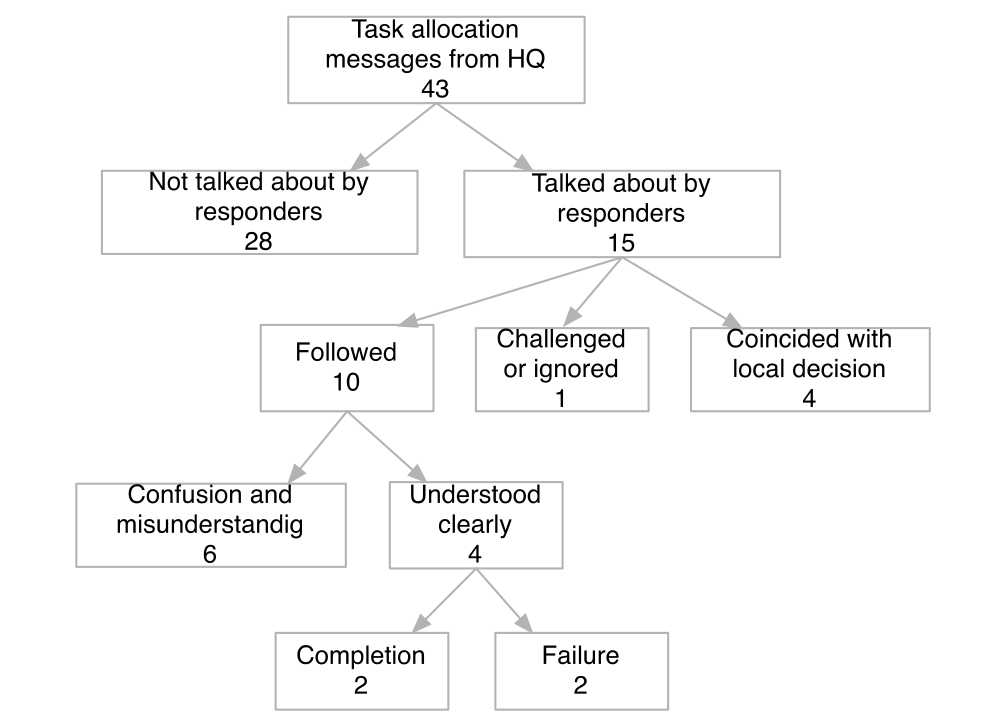
\includegraphics[width=1\textwidth]{img/study1/instructions}
  \caption{How responders addressed task allocation messages from HQ.}
  \label{fig:study1instructions}
\end{figure}

Directives index the instances of remote coordination of field responders by HQ. The observed response to messages is critical to understanding the relationships between local and remote coordination. The following episode depicts a team of three on their way to pick up fuel. Their path is blocked by radiation. Without a team, firefighter JH (on the left) has just joined soldier KY (on the right), and firefighter D2 who have just been allocated a task in a message by HQ. (Figure \ref{fig:study1ep11})\\

\begin{figure}[h]
  \centering
  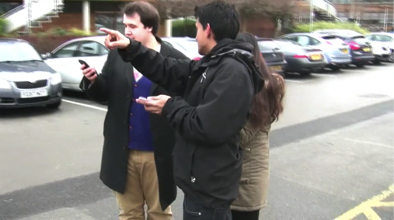
\includegraphics[width=1\textwidth]{img/study1/ep1/ep11}
  \caption{episode 1.1, JH (Behind Left), D2 (Middle Front), KY (Right behind)}
  \label{fig:study1ep11}
\end{figure}


\noindent \texttt{\textbf{Episode 1.1}\\
\textbf{KY:} ((reading out HQ message)) KY and D2, please walk fast to the junction and quickly return back ((laughs))\\
\textbf{D2:} Oh is that what we have to do? Ok so we have to run to (2.0) We need to work out where we have to run to first and then get (.) get it back. Which junction is that? If you run to the next (0.5) thing ((points)), and then come back (1.0) that would work (1.0) is it safer to go around?\\
}


\begin{figure}[h]
  \centering
  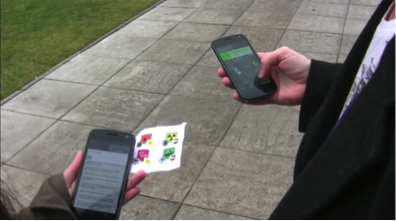
\includegraphics[width=1\textwidth]{img/study1/ep1/ep12}
  \caption{episode 1.1, KY (Left) , MF (Right) holding mobile phones}
  \label{fig:study1ep12}
\end{figure}


\noindent\texttt{\emph{[The team tries to go around the cloud but is stopped by radiation, realising their target is in the cloud. Meanwhile, D2 has left due to increased exposure.]\\}
\textbf{KY:} So we have to run! [through the radiation] \\
\textbf{JH:} Do we have to run through the (.) through the radiation? ((looking at map)) (Figure \ref{fig:study1ep12})\\
\textbf{KY:} Yah this is what the headquarters told us to do ((looking at messages)) \\
\textbf{JH:} I have a terrible feeling thats gonna kill us.\\
\textbf{KY:} But its gonna be meaningful ((laughs))\\
\textbf{JH:} We go around this corner, if it gets to half [referring to health] we should probably start running back.\\
\emph{ [KY JH begin running into the cloud] } (Figure \ref{fig:study1ep13})
}

\begin{figure}[ht]
\centering
\begin{minipage}[b]{0.45\linewidth}
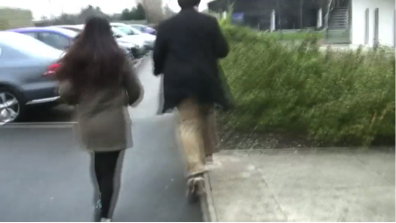
\includegraphics[width=1\textwidth]{img/study1/ep1/ep13}
\caption{episode 1.1, KY,JH running into cloud}
\label{fig:study1ep13}
\end{minipage}
\quad
\begin{minipage}[b]{0.45\linewidth}
 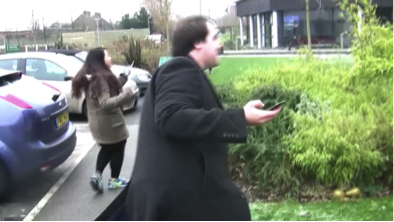
\includegraphics[width=1\textwidth]{img/study1/ep1/ep14}
\caption{episode 1.1, KY,JH turning around to escape from the cloud}
\label{fig:study1ep1-4}
\end{minipage}
\end{figure}

\noindent\texttt{\textbf{KY:} ((yells)) OH OH! It`s a hundred! [refers to radiation level]\\
\textbf{JH:} We are basically in the middle of it! We are basically in the middle of it!\\
\textbf{KY:} ((shouts)) I`m going back? Get the fuel first! Get the fuel first! Oh no! \\
\textbf{JH:} We are not prepared for that! I blame our HQ.\\
\emph{ [They turn around and run back out of the cloud without the fuel.] }(Figure \ref{fig:study1ep1-4})\\
}

This episode begins with a message by HQ attempting to help give directions to the target. D2`s response to the message is hesitant (`is that what we should do?'). His following question (`which junction is that?') suggests the referent in HQ`s message is not understood. They attempt to go around the radiation. They realise their target is in the cloud. They refer back to the message to support their intent to go into the cloud to attempt to save the target (`Yah this is what the headquarters told us to do'). Having run into the cloud, they refer to the Geiger counter and realise the exposure is too high. Meanwhile, their health is decreasing rapidly. They abandon the task and flee to safely, whilst JH expresses his frustration (`We are not prepared for that. I blame our HQ.').\\

First, the episode shows that geospatial referencing in messages can be problematic. It is unclear to the responders which junction HQ is referencing (and the responders do not ask for clarification), so they revise the route themselves. At the same time, they draw on the messages to justify their entering of the cloud. It does not occur to the responders that HQ allocated the task at an earlier time, before the cloud had covered the target. HQ does not update the responders on the increased danger, or revise their earlier task allocation. When the responder team fails to complete the task, they place blame instead of thinking self-critically.\\

\subsection{Local coordination without HQ}\label{sec:s1localcoordination}
As presented, field responders predominantly coordinated teaming and task allocation without HQ instructions. Recall that 14 targets are saved without HQ's instructions, versus only 2 targets that are saved with HQ's instructions. The following episode illustrates how field responders achieve coordination of teaming and task allocation locally. We join the action as BR and another responder are waiting at the drop-off zone without a compatible teammate, as MF and his teammate join and drop-off their target.\\

\begin{figure}[ht]
\centering
\begin{minipage}[b]{0.45\linewidth}
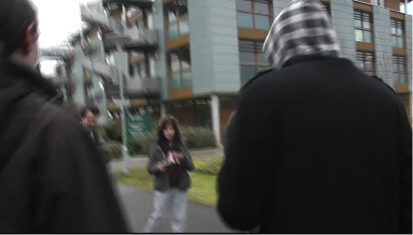
\includegraphics[width=1\textwidth]{img/study1/ep2/ep21}
\caption{episode 1.2, MF (right), BR (middle)}
\label{fig:study2ep21}
\end{minipage}
\quad
\begin{minipage}[b]{0.45\linewidth}
 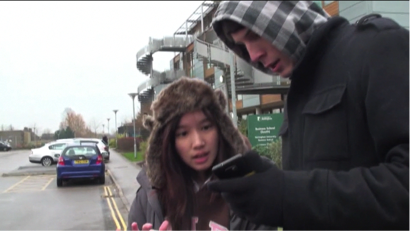
\includegraphics[width=1\textwidth]{img/study1/ep2/ep22}
\caption{episode 1.2, MF (right), BR (left)}
\label{fig:study2ep22}
\end{minipage}
\end{figure}

\noindent\texttt{\textbf{Episode 1.2}\\
\emph{[MF (on the right) and teammate walking towards BR (center)]\\}
\textbf{BR:} Any soldiers?\\
\textbf{MF:} I am soldier yeah.\\
\textbf{BR:} Would you like to pair with me? (2.0) to rescue a fuel?\\
\textbf{MF:} what are you after?\\
\textbf{BR:} I am a firefighter.\\
\textbf{MF:} Soldier and firefighter is fuel isn`t it?\\
\textbf{BR:} yeah.\\
\textbf{MF:} What can we get? (2.0) ((looks at screen)) this one in the center? ((points at screen))\\
\textbf{BR:} ((glances MF`s screen)) I think there are two people (the team D2,KY) going for that. I think we should go for this one ((points at screen)).\\
\textbf{MF:} We are going to get killed ((both laugh)).\\
\emph{[The team begins walking to target.]}\\
}

At the beginning of the episode, MF met BR, who was waiting at the drop-off zone without a compatible teammate. BR requested to team up with MF (``Would you like to pair with me? (2.0) to rescue a fuel?'') after MF identified himself as a soldier. BR and MF can then be observed sharing the screen of his device and using the map to identify potential targets (fuels) (Figure \ref{fig:study2ep22}). They realise one of fuel targets is already being pursued by another team. They agree on another target fuel to pursue. Note that messages do not play a role in this episode. It exemplifies how teaming and task allocation are achieved locally, without consulting HQ. \\

The next episode is a follow-up episode, which demonstrates how two teams resolve the conflict when they approach a same target.\\

\begin{figure}[h]
  \centering
  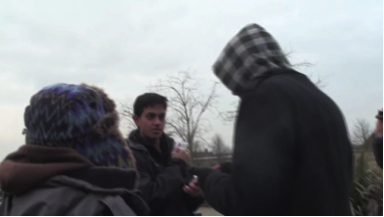
\includegraphics[width=1\textwidth]{img/study1/ep5/ep51}
  \caption{episode 1.3, MF (right), BR (left) met with D2 (middle)}
  \label{fig:intructions}
\end{figure}

\noindent\texttt{\textbf{Episode 1.3}\\
\textbf{D2:} we are told to get this fuel (target 1) from HQ.((pointing to screen))\\
\textbf{MF:} you are going to the fuel (target 1) we are aiming for, we thought you are going for this one (target 2).\\
\textbf{D2:} we were, until we got a message [from HQ] saying not to. \\
\textbf{MF:} you get that one (target 1), we get that one (target 2).((pointing to the two target locations))\\
\textbf{D2:} if you want get that one (target 2). It is somewhere in the building.\\
\emph{[The two teams split, proceed with the new target allocations]}\\}

At the beginning of this episode, the team (BR, MF) has decided to pursue (Episode 1.2) a target other than the one pursued by team D2, KY. However, instructed by HQ, MF and KY changed their target and met BR and MF on the way. The two teams then began to show their intended targets to each other. After they find they are heading to the same target, MF suggested a new allocation of tasks (``you get that one, we get that one.''). D2 then offered some information about the target location to the team MF, BR (``if you want get that one. It is somewhere in the building.''), suggesting he agreed with the new task allocations proposed by MF. \\

The two previous episodes show that how teaming and task allocation are achieved in a seemingly ``ad-hoc'' manner. By using the word `ad hoc', we stress the the actions of field responders are typically not planned ahead to great extend. The players often exchange information through conversations when co-located, and their `plan' is ready to be changed when new information is acquired. Take episode 1.2 as an example, while BR was waiting at the drop-off zone, she requested to team up with MF who happened to pass by. MF agreed to team up and then decided to aim for an available target that had not been aimed at by others. In episode 1.3, the two teams quickly came up with new task allocations when they found they were actually heading to the same targets. In the interview at the end of study, field responders also confirmed their ``ad-hoc'' behaviour in the interview:\\

\begin{quote}
\texttt{``Just save the closest target then just pair up and go to the other one'' }
\end{quote}

\begin{quote}
\texttt{``We just check, with that group, which target we can get. We see on the map to find the closet one we can get.''}
\end{quote}

% Add an episode from my part how the field responder resolve conflicts, suggest it is opportunistic. 



\subsection{Remote messages as a resource of situational awareness} \label{sec:study1awareness}
In the AtomicOrchid game, field responders need to be aware of what other responders are doing, where the `danger zone' is (the cloud), and where it is likely to move. Awareness of each other`s actions helps responders avoid conflicts in planning, while awareness of the danger zone is essential to survive. The following episode illustrates how responders use remote messages as a resource to gain situational awareness.\\

The episode takes place towards the end of game session B. The radioactive cloud has grown so much that navigation in the game area becomes increasingly difficult. MF is with a group of five responders, two of which are carrying an animal. The cloud is blocking their way towards the drop off zone; they stop.\\

\begin{figure}[h]
  \centering
  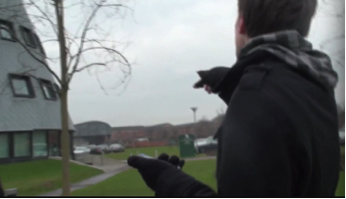
\includegraphics[width=1\textwidth]{img/study1/ep3/ep31}
  \caption{episode 1.4, MF pointing to a building}
  \label{fig:study1ep31}
\end{figure}

\noindent
\texttt{\textbf{Episode 1.4}\\
\textbf{MF:} ((reads message from HQ out loud)) There is another leak around Geospatial. (1.0) Which is Ah: so there`s a leak sprung up there. ((points)) Geospatial is like (.) that building right there. They say there is another leak. We should go all the way round (0.5) to the top left one, I think. (Figure \ref{fig:study1ep31})\\
}

MF brings up HQ`s message about the new leak, and suggests a route around the new cloud. The group ends up following MF`s route suggestion as a result. News of the new cloud, provided by HQ, enables the group to change their route to avoid danger. We commonly observed responders sharing information that provides situational awareness through face-to-face conversation. In the previous example, MF shared the message with a group of responders he was with already. The following example takes place between D2 and his teammate, as they are approached by JH, who is currently without a teammate.\\

\begin{figure}[h]
  \centering
  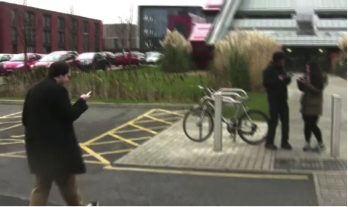
\includegraphics[width=1\textwidth]{img/study1/ep4/ep41}
  \caption{episode 1.5, JH (left) met team D2 (male, middle) and KY (female, right)}
  \label{fig:study1ep41}
\end{figure}

\noindent
\texttt{\textbf{Episode 1.5}\\
\textbf{JH:} Where are you guys heading? \\
\textbf{D2:} To get the fuel.\\
\textbf{JH:} Okay. The closest one to you? \\
\textbf{D2:} I believe so.\\
\textbf{JH:} Ya okay cuz I think the leak is somewhere near the other one and the army. [referring to building of Territory Army] (Figure \ref{fig:study1ep41})\\
\textbf{D2:} Oh (.) which one?\\
\textbf{JH:} They sent a message saying its between territorial army center. 
\textbf{D2:} We are trying to get the one here ((points)).\\
\textbf{JH:} The closest one. Okay.\\
}


Making use of the map as he approaches them, JH asks the others to clarify which fuel they intend to pursue (`the closest one to you?'). He proceeds to inform the team that the ``leak is somewhere near the other one''. D2`s response (`Oh, which one?') suggests they did not know this. In turn, JH elaborates on the location of the cloud, using an anonymous ``they'' to refer to the source of his information. ``They'' is likely to refer to HQ as they previously sent a message with the information of the cloud`s location. Conversational sharing of important information was a common resource responders employed to achieve and maintain situational awareness. However, requests for information in the messages channel were regularly not reciprocated with a response: out of 14 requests in session A, 8 were not responded to; and in session B, 14 out of 20 requests were not responded to (Table \ref{tab:adjpairs}).\\

\section{Discussion}
This section will present broader concerns that emerged from the game for the design of automated planning support.\\

\subsection{Division of labour}\label{sec:study1dlabour}
Firstly, the HQ plays an important role in providing situational awareness to the whole team. As the game mechanic provides the HQ exclusive access to the location of the radioactivity, the HQ managed to provide informational messages about the radioactivity to field players. Field players are able to pick up the information and spread it to other field responders through face-to-face conversations (Episode 1.2). Although HQ attempted to organise task allocations directly (through directives), their attempts are often problematic.  Although the field responders did not get too much planning support from HQ, they naturally organise themselves into small teams and carry out tasks. As shown in episode 1.4 and 1.5,  face-to-face conversation was vital for task and team organisation. We observed that co-located team members collectively make sense of the remote messages and game status shown on mobile screens. The decisions such as choices of team, targets and routes are  predominately made through local conversations.\\

The pattern of division of labour between field responders and HQ indicates the weak role of HQ in terms of task planning. The responder's choices of teams and targets seem to follow an ``ad-hoc'' manner as they heavily rely on face-to-face conversation, which can only happen when players are co-located. Despite some disruptions from the communication channel (confusions of geo-referencing, and out-dated HQ messages), field players seem to be able to find team-mates and generally avoid conflicts in their plans (e.g. avoid pursuing the same target) through local coordination. 


\subsection{Breakdown of remote coordination}\label{sec:study1breakdown}
The observed division of labour (Section \ref{sec:study1dlabour}) highlights heavy reliance on local coordination. To some extent, the heavy reliance on ``ad-hoc'' local coordination can partly be a result of the lack of remote coordination support. In other words, local coordination becomes important when system support for remote coordination is problematic. In a co-located setting, players can naturally make their actions observable and accountable to each other through conversations, body languages, gestures , screen sharing etc, and organise coordination activities reflexively. However, in the remote setting, the natural accountability of their activities become opaque. The game probe provides a set of functionalities supporting remote coordination, including GPS/map sharing, broadcasting. We have observed players utilise these functionalities to make sense of other team members' actions (see section \ref{sec:s1localcoordination}) and act accordingly. However, coordination with remote players is still problematic which can be evidenced by the lack of response and acknowledgements to requests in the messaging channel (Section \ref{sec:adjpairs}); and the misunderstanding and confusions observed when field responders try to follow the directives from HQ (Section \ref{sec:study1directives}).\\

We suggest that future planning support should properly support remote coordination in a way that facilitates accountability among distributed team members. Section \ref{sec:study1requirements} discuss some detailed requirements of remote coordination support drawn from the field observations. The next section in particular,  expands on the design requirements that can enhance remote coordination in a way that supports natural accountability of human activities.\\

%{ The natural social order that employed by the team members to make sense of the task environment. Players are observed to constantly revealing to others their action and plans via face to face conversation. CSCW concern that Geo-spatial distribution distributed  hinders team member's attempt maintain accountability . The lack of response in the communication channel shows that. The form of communication in this study appears to be unable to support the team member's accountability. The missing of remote coordination and the weak role of HQ in the planning activities may indicate communication breakdown, which can also be confirmed by a number of observations of understanding and confusions in the communication channel (see x.x.x).\\From this perspective, the domination of local coordination . Some of the reasons? %}

\subsection{Implications on computational support}
%[connect to situated planning by Lucy suchman] it is a kind of situated action. \\
% It is important that we do not treat human plan in an inferir way. They are about to leverage all the resources avalible to make deblibration on their actions. Supporting them a plan will be the same as augmenting their resources. How the team organsie their activities around this resouces can be makde subjuct of study. and study about that can lead to interaction design that support situation

To some extent, the observation of ``ad-hoc'' local coordination is aligned with the view of situated actions. As a whole team, players form and disband teams without holistic plans prior to their actions. Players are observed to have conversations about their status, on-going activities when they meet up. Local decisions for next moves are often made during the conversations.  Information from mobile interface (e.g. player locations, radiation readings and messages) are often brought to conversions as resources in the context of their situated actions. \\

The lack of plans may indicate the lack of optimisation of team task allocation. The multi-agent coordination algorithms (e.g. \citep{Ramchurn2010}) aims to support the team by producing computationally optimised plans for responder teams. However, design of the planning support may not be straightforward. \\

Firstly, there is a danger of imposing an inappropriate ``work model'' (assumed by agent support) on the human team. Studies of \ac{CSCW} systems \citep{Bowers1994} raise a concern that the work model held by the technological system sometimes comes into tension with the natural human workflow achieved through methods internal to the work. In particular, current division of labour between HQ and field responder suggest that HQ plays a supportive role (providing situational awareness). However, a centralized coordination algorithm may need to coordinate the whole team, requiring every player to follow top-down instructions to reach a global optimum of resource allocation. In that case, the role of the control room may need to change and it is unknown whether the change will disrupt or support human workflow. \\

Apart from disruption of human workflow, there is also a danger of the supporting system imposing a planning model on human teams. \cite{Suchman1987} suggests that human's situated action should not be simply treated as a inferior version of scientific planning model. Following the view of situated actions, supporting human's actions are not as simple as providing an optimised plan to execute. A plan for human teams is only one of the resources that humans can utilize for their deliberation on their actions. Therefore, the role for the system is to provide plans (as an extra resource) in a way that supports the human's situated actions. \\

Adopting the view of human agent interaction, we can treat a plan support system as a teamwork agent.  Achieving mutual intelligibility between the agent and the human team can also be a major design challenge. Plans generated by a planning agent can only a representation of possible actions and effects based on simulations. How the responders make use of plans can be highly dependent on situations in which mutual intelligibility plays an important role. For example, it would be problematic if globally optimised choices conflict with the ``ad-hoc'' choices that are obvious for human field responders. We cannot assume either the agent or human choice will be always correct, perhaps neither of them can take an authoritative role. Therefore, we need to carefully design the interaction between human and agent to ensure that they maintain mutual intelligibility so that informed collective decisions can be reached.  \\

%which is often the main concern of multi-agent coordination algorithm. However, the dominance of ``ad-hoc'' local coordination indicates the absence of the notion of resource optimisation. In a sense, it opens opportunity for computational support, but it also highlights some potential challenges for such support system. 


\section{Design Requirements}\label{sec:study1requirements}
Drawing on the problems observed in remote coordination (Section \ref{sec:study1breakdown}), we now discuss the detailed design requirements that enhance remote coordination. The embodied game probe embedded responders in a challenging setting. They needed to communicate effectively to make time critical decisions on teaming and task allocation, both locally in the field as well as remotely through messaging. Field responders physically engage and navigate the environment to perform tasks while maintaining awareness of risk and danger. The data reveals multiple challenges for team coordination involving communication and decision-making. \\

\textbf{Sharing of local decision-making}. The study showed that teaming and task allocation were predominantly organised locally among field responders, in an ``ad-hoc'' manner. Despite the fact that HQ attempted to coordinate task allocation remotely, few of these directives were brought to conversation locally. Only 2 out of 16 tasks that field responders completed were remotely allocated by HQ (Figure \ref{fig:study1instructions}). Although players are able to smoothly conduct local coordination, local coordination heavily relies on and is limited by the face-to-face conversations, which means some conflicts of planning can only be found and resolved when players meet each other (e.g. episode 1.3). Therefore, local decision-making can benefit from a shared picture of team-wide planning decisions. We thus argue that local decision-making needs to integrate capabilities to enable team-wide sharing of the local decisions.\\

\textbf{Coordinate resources}. While field responders made decisions on teaming and task allocation in a seemingly ad hoc fashion, game data reveals how field responders draw on resources to achieve situational awareness in order to coordinate successfully. A common understanding of the location and movement of the radiation cloud was achieved by sharing information from game messages verbally in a local group. Face-to-face talk was an essential resource for relaying information from the Mobile Responder App to teammates, such as radioactive exposure, others` whereabouts, task status, and other monitoring of the broadcast messages. Future planning support systems need to take into account that such coordinate resources are likely to be comprised of digital as well as embodied human resources. \\

\textbf{Geospatial referencing} The results show that geospatial referencing was problematic in various ways, particularly in directive messages sent to the field players. Participants had different levels of knowledge of the campus, which made understanding of landmarks references uncertain. Some participants also struggled with making sense of north/south/east/west directions in relation to their current position and orientation. To deal with misunderstandings, players had to ask for clarification via messages or spend valuable time discussing the reference locally in order to understand it. Consistent with the findings of \cite{Toups2009}, designers need to think carefully about how the presentation layer of such systems may be augmented with information that facilitates geospatial referencing (e.g., grids, labelling etc.) to facilitate human in addition to machine readability. \\

%Freshness of messages. Problems arose from erroneous instructions or otherwise out-dated messages sent to field responders. In one case HQ sent a message in which two players with non-compatible roles were instructed to team up. This was particularly costly, as the players attempted to team up, and lost valuable time until they realised the game mechanics barred them from forming a team.\\

\textbf{Freshness of messages} As demonstrated in one of the episodes, reading out-dated messages in a dynamically changing environment can contribute to responders taking dangerous actions that they believe to be safe, because they do not realise that the information is out-dated. However, in most cases, recipients managed to identify temporally irrelevant messages, and thus avoided following them. To reduce confusion about message freshness, such systems should address these issues at the UI level, both for responders and for HQ. Develop functionality to flag messages as out-dated, to retract incorrect messages, or highlighting up-to-date messages. 

% System support of shared representation of plans and status.

%Thus, our findings support the use of fresh social media as a source of information for disaster response, despite problems that can arise with validation, because crowdsourced information will in many cases provide better coverage than official sources.\\

\textbf{Acknowledgement of messages} In most cases, field responders did not acknowledge or respond to messages sent by the HQ. This was particularly problematic for directives (task allocation), as task status and field responder compliance often had to be inferred by observing their location updates on the map. This consumed HQ attention, with negative impact on HQ`s overall work on state assessment and task planning. Observations in the field suggest that the physical demands (e.g., co-located team movement through terrain at speed) and cognitive demands to maintain situational awareness (e.g., monitoring of radioactivity and messages) are likely factors that explain lack of acknowledgement.\\

%data

As a result, user interfaces that enable and encourage field responders to quickly acknowledge HQ messages, with minimum cognitive load, should be considered for messaging in such systems in such high demand settings. For effective team coordination in disaster response, interface and workflow designs need to factor in cognitive load and task demands for effective information distribution.\\


\section{Summary}
The objective of this study is to unpack how human teams coordinate in the time and space constrained task setting. In particular, we focussed on a scenario in which responders coordinate role-based teaming and spatially distributed task allocation and execution using a real-time location and messaging system, with no automated planning support.\\

We presented the design and study of the AtomicOrchid game as a mixed-reality game probe to investigate challenges for team coordination in a setting in which participants experience both physical strain through bodily activity, and cognitive challenge through time pressure and task complexity. We use mixed-reality game probes as a platform for investigation of concomitant socio-technical issues: handling of mobile devices to communicate and maintain situational awareness (messaging, sensing, interaction, and display) intersect with face-to-face interaction, whilst the physio-cognitive challenges created through game mechanics and environment induce stress. We created a setting that allows exploring requirements to support team coordination of relevance to time-critical coordination domains such as real disaster response.\\

Findings from interaction analysis of field observations, triangulated with log files, reveal how field responders achieved coordination by drawing on local face-to-face conversation with fellow responders, and situational information provided by the interactive map, the Geiger counter, and the messages sent by HQ. Drawing on these findings, we highlight challenges of introducing automated planning support into the socio-technical setting of \ac{AO}. We also generate requirements for supporting team coordination, emphasising the roles of local coordination, decision-making resources, geospatial referencing and message handling. Most of the requirements are feed into the refinements of \ac{AO} system in later studies, which help to reduce influence of non-agent related design factors. \\

% These requirements inform future work on building planning support system by emphasising the role of human interaction in team coordination in time-critical settings.\\

%************************************************
\chapter{AtomicOrchid Study 2: The Human On-the-loop Design}\label{ch:studytwo} % $\mathbb{ZNR}$
%************************************************
This chapter presents the second iteration of AtomicOrchid field trials. In this study, a planning agent is integrated into the system by following a human on-the-loop interaction design, in which the HQs only monitor the planning agent and occasionally intervene. The purpose of the trials is to investigate socio-technical issues related to human agent interaction. Interaction analysis is conducted to examine log data and field observations revealing how human agent interaction plays out, in turn, revealing the process by which players interpret and negotiate the agent`s guidance as well as how these are intertwined with social dynamics of the teams.

\section{Introduction}\label{sec:studytwointroduction}
% Task planning in teams can be complicated by both spatial and temporal constraints, particularly in time-critical task domains such as \acf{DR}. In a \ac{DR} setting, responder teams have to coordinate sparse resources and personnel to prioritize geographically distributed tasks, forming and disbanding teams dynamically to carry out \ac{DR} operations \cite{Chen2005}. Multi-agent researchers have devised a number of agent coordination algorithm to coordinate task allocations for multi-agent systems, which can be adapted to support planning activities of \ac{DR} teams. \\

% However, these algorithms typically model humans as computational agents with respective capabilities, for example to dynamically allocate teams of agents to tasks in order to maximise an objective (e.g., number of lives saved), taking into account other aspects of the real world (environment, infrastructures, victims, etc.) \cite{Ramchurn2010a}. Therefore, the quality of the planning results can be constrained by limited assumptions of human behaviour (e.g., human psychosocial characteristics, movement, and learning ability) and real world environment \cite{Armenakis2012}. These limitations highlight importance of human input in the planning process. Thus, we argue that effective collaboration between human and agent is required to produce and execute high quality plans in the disaster setting. . \\

In order to support effective Human agent collaboration, two patterns of interaction design (Human On-the-loop and In-the-loop) are presented in section \ref{sec:patterns}. In this study, the planning agent is integrated into the AtomicOrchid system with a straightforward Human On-the-loop design (Figure \ref{fig:study2OnTheLoop}). This design assumes minimal Headquarters intervention, that is, the agent can directly interact with field responders to generate and implement plans without constant involvement of HQ. The interaction design is aimed to facilitate a pattern of division of labour, in which a planning agent routinely assigns tasks to distributed responder teams, while human coordinators (the HQ) monitor and support the task execution by responding to arising contingencies. The agent is designed in a way to take into account simple human feedback, i.e., a field responder can either reject or accept their task assignment. The agent will consider the feedback for the next iteration of task assignment.\\

\begin{figure}[h]
  \centering
  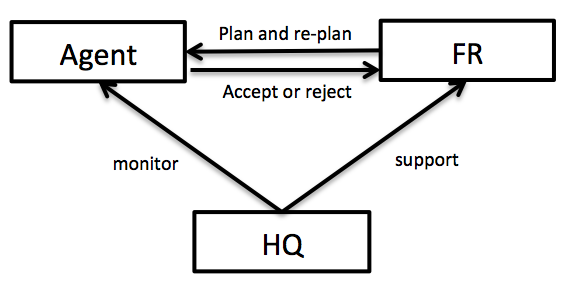
\includegraphics[width=0.7\textwidth]{img/approach/OnTheLoop}
  \caption{On-the-loop interaction design}
  \label{fig:study2OnTheLoop}
\end{figure}

This study uses the agent integrated version of AtomicOrchid as a probe to unfold socio-technical issues in human-agent interaction, with focus on the implications of the Human On-the-loop design on human team performance. More specifically, this chapter addresses the following research questions on how agent guidance affects the social organisation of team performance:\\

\begin{enumerate}
\item How do human teams respond to being instructed by an agent, particularly on switching teams and tasks?\\
\item The planning agent makes decisions based on limited assumptions about human behaviour, but what are the hidden costs of human behaviour that the agent does not take into account?\\
\end{enumerate}

Findings from the study highlight the social processes in which members interpret, negotiate, and manage the agent guidance within the social dynamics of teams. We discuss the division of labour between humans and teams and the hidden costs of instructions that suggest team reformation and interrupt on-going tasks. We conclude this chapter with a number of emerging interaction design recommendations to consider when building planning support systems for human teams, which emphasises the need for common ground between humans and the agent, facilitate accountability between team members, and balance responsibilities between humans and the planning agent appropriately.\\


% ===== from CTS need adaptation =====
%We present a field trial of how instructions from an intelligent planning agent are dealt with by distributed human teams, in a time-critical task setting created through a mixed-reality game. We conduct interaction analysis to examine video recorded field observations and game log data. The findings highlight the social process by which players interpret and negotiate the agent guidance as well as how these are intertwined with social dynamics of the teams. The insights can be used to develop an understanding of interactional issues around automated team instructions and inform the design of human-centred planning support systems. \\

%Task planning in teams can be complicated by both spatial and temporal constraints, particularly in time-critical task domains such as disaster response (DR). In a DR setting, responder teams have to coordinate sparse resources and personnel to prioritize geographically distributed tasks, forming and disbanding teams dynamically to carry out DR operations [4]. For example, teams of fire fighters and medics are required to extinguish a fire and to provide first aid, while teams of soldiers and transporters may be needed to clear rubble. These teams, in turn, may need to disband and reform dynamically to perform new tasks and to adapt their planning to uncertainties in real time. Whilst an `optimal' plan of team formation and task allocation may help minimise loss of lives and properties, making optimal plans in real time can be complicated and time-consuming due to large numbers of incidents and responders. To address such coordination challenges, multi-agent research has developed a number of smart coalition formation algorithms to computationally support planning in time-critical task settings [3,16]. These algorithms typically model humans as computational agents with respective capabilities, for example to dynamically allocate teams of agents to tasks in order to maximise an objective (e.g., number of lives saved), taking into account other aspects of the real world (environment, infrastructures, victims, etc.) [14]. \\

%However, most of these smart algorithms are based on limited assumptions about human behaviour (e.g., human psychosocial characteristics, movement, and learning ability) [18], and have only been evaluated in computational simulations. In our work, we investigate agent-based planning support in the real world. Specifically, we study the social implications of the division of labour between agents and real human teams. In more detail, while coalition formation assumes leaving and joining new teams as an unproblematic process, we study in depth the social, interactional consequences of agent-based instructions that require team formation. For example, Personal preference and social norms may imply that dynamic team formations have a hidden social cost that may impact team performance. \\

%We present AtomicOrchid, a mixed-reality game probe of the ways in which human teams respond to agent guidance. The probe is designed to create a socio-technical setting in which distributed teams and a planning agent work collectively to save locally dispersed targets on the ground. The planning agent runs a coalition formation algorithm to help allocate tasks optimally to the teams. Our analysis reveals social implications of agent support for human teams. In turn, implications for interaction design are discussed that may improve team performance. More specifically, this paper addresses the following research questions on how agent guidance affects the social organisation of team performance:\\

%How does division of labour play out between humans and agents and how should it be scaffolded by design? 
%How do human teams respond to being instructed by an agent, particularly on joining and leaving teams?
%The planning agent makes decisions based on limited assumptions about human behaviour, but what are the hidden costs of human behaviour that %the agent does not take into account?\\

%Findings from the study highlight the social processes in which members interpret, negotiate, and manage the agent guidance within the social dynamics of teams. We discuss the division of labour between humans and teams; the hidden costs of instructions that suggest team reformation and interrupt on-going tasks. We conclude the paper with a number of emerging interaction design recommendations to consider when building agent-based support systems for human teams, which emphasise the need for common ground between humans and the agent, facilitate accountability between team members, and balance responsibilities between humans and the planning agent appropriately. 

\section{System Evolution}\label{sec:studytwosystem}
Compared to study 1 (Chapter \ref{ch:studyone}), the system has evolved to provide agent planning support with an On-the-loop interaction pattern. This section gives a description of the changes of system, which covers integration of a planning agent, implementation of a quick feedback system, and improvement in both HQ and mobile interface.

\subsection{The planning agent}\label{sec:studyoneagent}
One major change of the system is the integration of a planning agent into the AtomicOrchid platform. The planning agent is developed by ORCHID research partner Wu Feng, Savapali Ramchum, and detailed in section \ref{sec:appagent}. \\

%The coordination problem (Section \ref{sec:gameRatinale}) of the AtomicOrchid is modelled using a Multi-Agent Markov Decision Process (MMDP) that captures the uncertainties of task execution, extending earlier work \cite{Ramchurn2010}. The modelling allows responder actions to be delayed or to fail during the rescue process. The MMDP modelling leads to a large search space, even with a small-sized problem. Hence, we devised an approximate solution to save computation time, which can be executed to support real time planning \cite{Wu2015}. The planning algorithm takes into account both time (cloud and human movement speed) and spatial (path planning for responders) constraints. The planning algorithm run by the planning agent produces high quality task allocations that minimise the travelling distance of first responders, and maximise the number of targets rescued. Before the agent was deployed to support human teams in the game setting, computational simulations were done by Wu Feng to benchmark our MMDP algorithm against greedy and myopic methods (Table  \ref{tab:alg}). The results confirm that our algorithm produces efficient task allocations.\\

The planner, implemented by Java, is wrapped in a PHP server framework and deployed on an independent server separate from AtomicOrchid. The planner server exposes a HTTP interface for AtomicOrchid to request plan. Each plan request issued by AtomicOrchid is appended with updated game status, which includes players' health, distribution of radioactive cloud and locations of players, and targets. Based on the updated game status, the agent will produce an optimised task allocation and return it to AtomicOrchid. The plan requests are triggered frequently in game sessions so that the task allocation can be frequently adjusted according to task execution status. In this study, plan requests (and thus re-planning) is triggered by two kinds of game events:\\


\begin{enumerate}
\item Completion of task. On successful rescue of a target, a new plan (i.e., allocation of tasks to each responder) is requested from the agent.\\

\item Explicit reject. On rejection of a task allocation by any of the first responders, a new plan is requested.  The feature of rejection is part of a feedback loop between human and agent, at will be introduced in next section.\\

\end{enumerate}

\subsection{A feedback loop}\label{sec:study2feedback}
The feedback system is part of the On-the-loop interaction design, which enables the agent to take into account simple human feedback. It is also partly inspired by a requirement generated in study 1, which highlights the importance quick acknowledgements from field responders. The feedback system can be seen as a system mechanism for the field team to provide quick responses to the planning agent. This section goes through the implementation details of the feedback loop.\\

Once a plan is received from the agent, the AtomicOrchid game engine splits the plan for a given team into individual task allocations and sends these to each responder`s mobile app (Figure \ref{fig:handlingplans}). The app displays the task allocation in a pop-up and details it in the task tab, including: i) the responder to team up with, ii) the allocated target (using target id), and iii) the approximate direction of the target (e.g., north, east) (Figure \ref{fig:study2mobiletask}).\\

\begin{figure}[h]
  \centering
  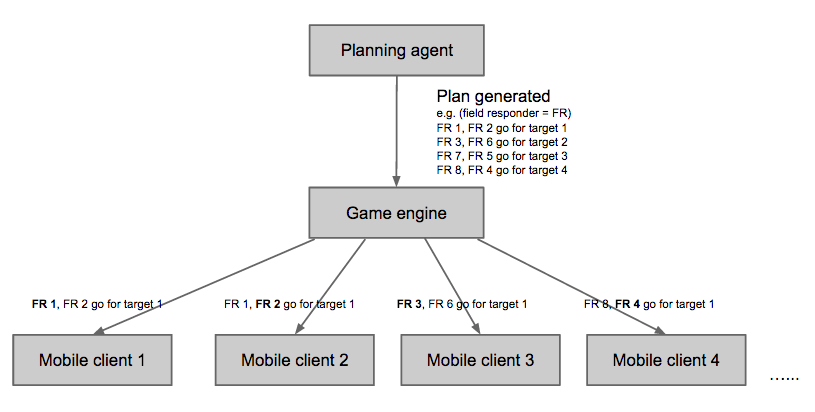
\includegraphics[width=1\textwidth]{img/study2/system/dealingwithplans}
  \caption{Game engine handling plans from agent}
  \label{fig:handlingplans}
\end{figure}

On receiving an instruction from agent, the field responder can choose to either reject or accept the instruction (Figure \ref{fig:study2mobiletask}). In the case of rejection, a new plan will be requested and the agent will consider the feedback for the next iteration of task assignment. More importantly, the rejected allocation is used as a constraint within the optimisation run by the planner agent. For example, if two responders (a medic and a soldier) were allocated a task and the solider rejected it, the planning agent would return a new task allocation with the constraint that this soldier should not be allocated this task. The instructions sent to field responders are also displayed in the HQ interface for monitoring purposes. The task allocations are represented as yellow lines connecting players and their targets (Figure \ref{fig:study2HQ}). Only one task allocation is displayed at one time, HQ player can click on the `show' task button on the player status panel (top right) is to chose whose task to be shown.  \\

\begin{figure}[h]
  \centering
  \fbox{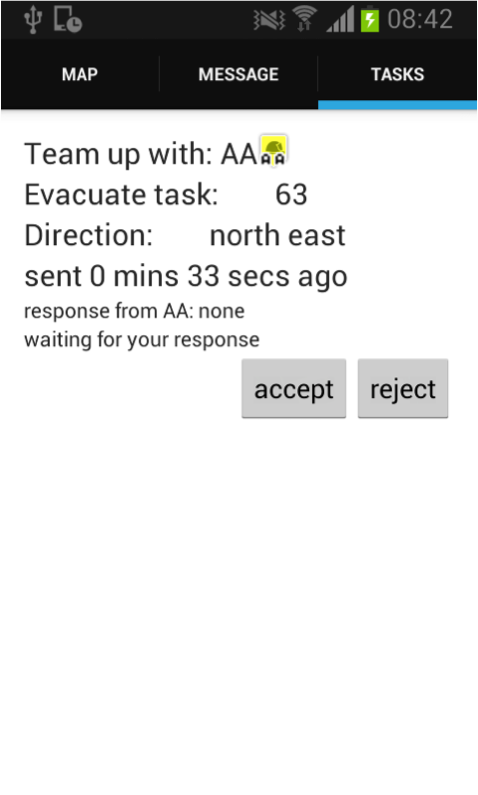
\includegraphics[width=0.4\textwidth]{img/study2/system/mobiletask}}
  \caption{Mobile task interface in study 2}
  \label{fig:study2mobiletask}
\end{figure}

\begin{figure}[h]
  \centering
  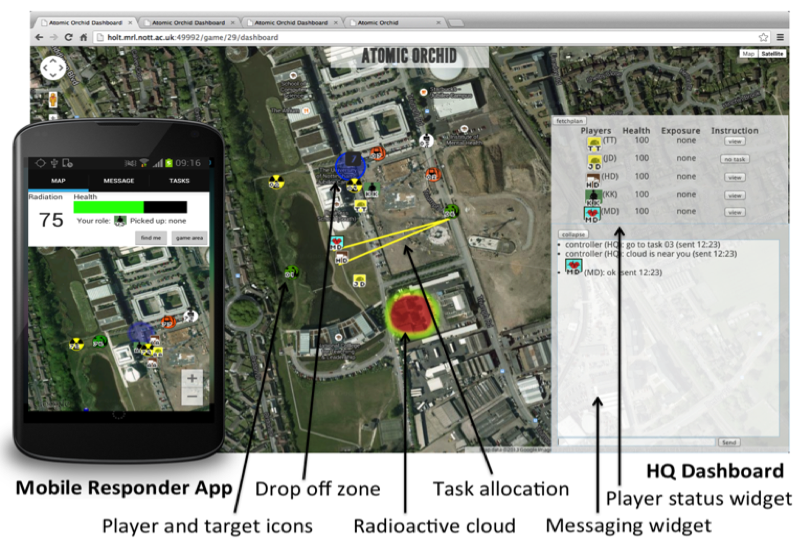
\includegraphics[width=1\textwidth]{img/study2/system/HQ}
  \caption{HQ and mobile interfaces in study 2}
  \label{fig:study2HQ}
\end{figure}


\subsection{Interface improvements}\label{sec:studytwointerface}
Apart from the agent integration and feedback system, two small modification of the interface were inspired by the requirements generated in the previous study (Section \ref{sec:study1requirements}). Firstly, all icons of targets are now marked by a unique target number for HQ and field responders to cross-reference. Secondly, all the messages are labelled by timestamps for players to help identify outdated messages (Figure \ref{fig:study2mobilemsg}).\\

\begin{figure}[h]
  \centering
  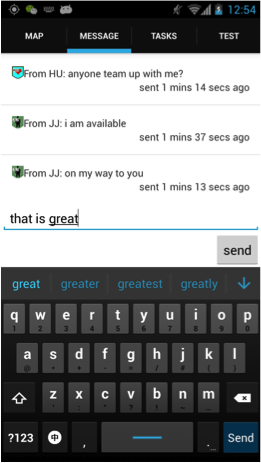
\includegraphics[width=0.4\textwidth]{img/study2/system/mobilemsg}
  \caption{Mobile message interface in study 2}
  \label{fig:study2mobilemsg}
\end{figure}

\section{Study Design}
Study participants were recruited through posters and emails. A total of 18 participants were recruited for 2 sessions of Game play (Appendix \ref{app:demo2}). For each session, there was 1 HQ player and 8 field players. All participants were reimbursed with 15 pounds for 1.5 hours of study. The majority of participants were researchers and students of the local university. The procedure of study is the same as the one described in study 1 (Section \ref{sec:study1procedure} )\\

The game area was the same as for study 1 on the local university campus (Appendix \ref{app:area2}), 400 by 400 meters, without heavy traffic. The terrain of the game area includes grassland, a lake, buildings, roads, and footpaths and lawns. There are two drop off zones and 16 targets. There were four targets for each of the four target types. The pattern of cloud movement and expansion was the same for both game sessions, and it is the same as for study 1.\\

%In this study, we aimed to probe a straightforward [interaction design] between a planning support agent and human teams (Fig. 1). The interactional design is designed to facilitate the division of labour between humans and agent: a planning agent routinely assigns tasks to distributed responder teams, while human coordinators (the HQ) monitor and support the task execution by responding to arising contingencies. The agent is designed in a way to take into account simple human feedback, i.e., a field responder can either reject or accept their task assignment. The agent will consider the feedback for the next iteration of task assignment. \\

%By examining the socially organised interaction between team members occasioned by this interactional arrangement, we aimed to explore social implications of human-agent interaction. In turn, these inform the design of agent-based systems. In the following, we describe the study in detail. \\

%A real-time algorithm was developed to support the coordination problem created by the game mechanic. The coordination problem (described in IV, A) is modelled using a Multi-Agent Markov Decision Process (MMDP) that captures the uncertainties of task execution, extending earlier work [15]. The modelling allows responder actions to be delayed or to fail during the rescue process. The MMDP modelling leads to a large search space, even with a small-sized problem. Hence, we devised an approximate solution to save computation time, which can be executed to support real time planning. The planning algorithm takes into account both time (cloud and human movement speed) and spatial (path planning for responders) constraints. The planning algorithm run by the planning agent produces high task allocations that minimise the travelling distance of first responders, and maximise the number of targets rescued. Before the agent was deployed to support human teams in the game setting, computational simulations were used to benchmark our MMDP algorithm against greedy and myopic methods (see Table 1). The results confirm that our algorithm produces efficient task allocations. \\

%In their mission to rescue all the targets from the disaster space, a centrally located HQ and the planning agent support the responders on the ground. In what follows, we present the player interfaces and the interactions with the planning agent. A demo video can be viewed at http://bit.ly/1ebNYty.\\

%First responders are equipped with a mobile responder tool (Fig. 2) providing sensing and awareness capabilities in three tabs (Geiger counter, map, messaging and tasks). The first tab shows a reading of radioactivity, player health level (based on exposure), and a GPS-enabled map of the game area to locate fellow responders, the targets to be rescued and their drop off zones. The second tab provides a broadcast interface to message fellow first responders and the HQ. The third tab shows the team and task allocation dynamically provided by the agent that can be accepted or rejected. Notifications are used to alert both to new messages and task allocations.\\

%HQ controls the HQ dashboard that provides an overview of the game area, including responders real-time locations (Fig. 2). The dashboard provides a broadcast messaging widget, and a player status widget so that the responders exposure and health levels can be monitored. HQ can further monitor the current team and task allocations to individual responders by the planning agent (by using buttons in the player status widget). Crucially, only HQ can see the radioactive cloud, graphically depicted as a heatmap. The rationale was to entice frequent communication between field responders and HQ.  \\

\section{Data analysis and results}\label{sec:study2analysis}
Here, we present findings from interaction analysis that reveal how team coordination was achieved. Overall, responders rescued 12 and 11 targets in sessions A and B respectively, out of 16 targets in total per session. No player was incapacitated in the two sessions. The planning agent sent a total of 51 instructions (Figure \ref{fig:study2agentInstructions}), 24 of which are accepted and 11 of them are rejected. The remaining 16 instructions do not receive complete responses (at least one of the player did not reply). A total of 21 instructions were finished successfully, versus only 2 of the targets are saved without agent instructions. Of the the 19 instructions that were unsuccessful, some were ignored or violated by players and some were overridden by the agent in the replanning process due to change of circumstance.\\

\begin{table}[h]
\footnotesize
\begin{tabular}{llll}
\multicolumn{1}{l|}{} & Saved targets & Incapacitated players & Average Health \\ \hline
\multicolumn{1}{l|}{Session A} & 12 (out of 16) & 0                    & 80/100             \\ 
\multicolumn{1}{l|}{Session B} & 11 (out of 16) & 0                    & 82/100             \\ 
\end{tabular}
\caption{Overview of game results}
\label{tab:gameResults1}
\end{table}

\begin{figure}[ht]
 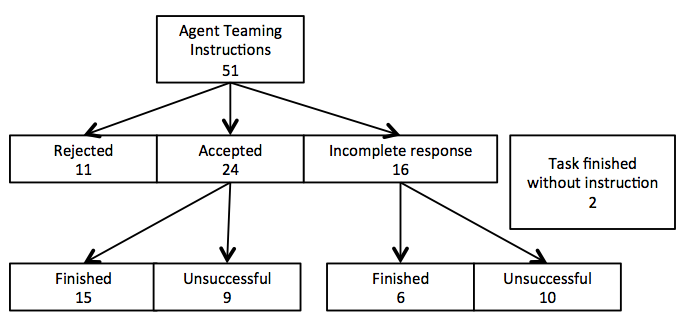
\includegraphics[width=1\textwidth]{img/study2/system/agentInstructions}
\caption{Overview of agent instructions}
\label{fig:study2agentInstructions}
\end{figure}

In what follows, we presents selected episodes of game play to reveal how teams accomplish the tasks in the rescue mission, particularly focusing on the social organisation of interaction with and around the agent instructions (Appendix \ref{app:vis2}). The order in which we present the episodes follows the common practice of moving from exhibits of typical/unproblematic instances, via more complex/difficult instances, to exhibits that display problematic interaction or even complete breakdowns. The episodes in later sections will be presented with a standard orthographic notation detailed in section \ref{sec:aprIA}.

% In the episodes, players can be uniquely identified by their initials. Targets are denoted by their unique numeric target id. Task assignments from the agent are represented as two initials and one target id connected by a rightward arrow. For example, the notation PC, CR -> 22 means player PC and CR are instructed to team up and go for target 22. A standard orthographic notation \cite{Jordan1995} is complemented by timestamps [0:00], and system messages from remote players and HQ.  

\subsection{Assigning task assignments to existing teams}
The following episode depicts a team of two dropping off a target and planning the next step.\\

\noindent\texttt{\textbf{Episode 2.1}\\
\emph{[0:00] The team dropped off a target.}\\
\textbf{PC:} I think we dropped off now. Ok. \\
\emph{ [0:07] The team receives a new agent instruction: PC, CR -> 22}\\
\textbf{PC:} I have a task now (3.0) ((studying screen)), I need to go with CR to 22. Are you CR? (Figure \ref{fig:study2ep11})\\
\textbf{CR:} Yes.\\
\textbf{PC:} go 22.\\
\textbf{CR:} We have done 22.\\
\textbf{PC:} Oh (1.0), no (2.0) 22 is there ((pointing to direction of 22)), Let`s go ((PC leads the way, they start walking to 22))\\
\textbf{PC:} Right this way. (Figure \ref{fig:study2ep12})\\
\emph{ [0:28] The team finishes the task assigned by the agent.}\\
}

\begin{figure}[ht]
\centering
 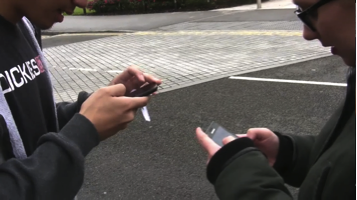
\includegraphics[width=0.7\textwidth]{img/study2/ep1/ep11}
\caption{ep 2.1, CR (Left) and PC (Right) studying screen together after drop off.}
\label{fig:study2ep11}
\end{figure}

\begin{figure}[ht]
\centering
 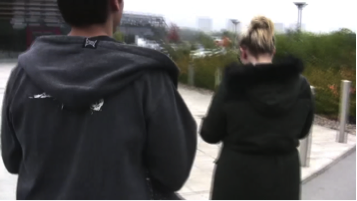
\includegraphics[width=0.7\textwidth]{img/study2/ep1/ep12}
\caption{ep 2.1, PC (Right) leading the way to new target.}
\label{fig:study2ep12}
\end{figure}

At the beginning of this episode, the team (PC, CR) drops off a target at a drop off zone. Player PC vocalises that they have finished the task (``I think we dropped off now. OK'').  After about 7 seconds, PC says she received a new task allocation from the agent (``I have a task now''). PC confirms the initials of the other player (CR), and suggests CR to join her to go for target 22. The action is consistent with the agent instruction (PC, CR -> 22), suggesting that PC has read through the instruction and decided to follow it. CR said that they have already finished target 22 (``We have done 22''), which indicates he is confused about the current task allocation. PC resolves the confusion by pointing in the direction of 22 and repeating to go for it. Later, the team successfully drop off target 22 as instructed by the agent.\\

The episode shows how an agent instruction is brought up and followed by a team in relative straightforward manner. The instruction was delivered immediately after the drop off of a previous target (7 seconds after). PC successfully locates the new target in the instruction and leads the team to pick it up. Although CR is confused at first, PC manages to rectify CR`s mistake and they finish the task successfully. \\

This episode is a typical case of task assignment to existing teams, i.e. the agent sent a new task to a team immediately after they finished their previous task. Out of a total of 51 agent instructions, 23 fall into this category. The rate of compliance is high for these cases of task assignment to existing teams (21 out of 23; 91\%). \\

\subsection{Task assignments involving team reformation}
Unlike episode 2.1, sometimes the agent instruction implies players need to disband and form new teams after finishing their previous task, in order to enact the computationally optimal plan. 10 out of 51 agent instructions fall into this category (Table \ref{tab:compliancerate}). The compliance rate of instructions that require reteaming (50 percent) is substantially lower than compliance of instructions where players can stay in the same teams (91 percent). The following episode depicts a typical case in which team reformation fails.\\

\begin{figure}[ht]
 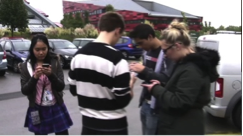
\includegraphics[width=0.8\textwidth]{img/study2/ep2/ep21}
\caption{episode 2.2, players from left to right: LT, SS, CR, PC. LT  walking around the team, her body orientation suggesting attempts to leave the group.}
\label{fig:study2ep21}
\end{figure}

\noindent\texttt{\textbf{Episode 2.2}\\
\emph{[0:00] After a target drop off, LT and SS joined PC and CR at drop off zone.} \\
\emph{ [0:24] HQ sent message A: LT, if you think you have the stamina to run to 10 around the north of the lake do so now with a firefighter. }\\
\emph{ [0:28] Agent instruction received:  NK, LT -> 16 }\\
\textbf{LT:} They said ((reads out aloud HQ message A)) \\
\emph{[0:35] CR ((facing LT)): Shall we go get 10}\\
\textbf{LT:} Mine is 16. \\
\emph{[0:38] HQ sent message B: Avoid 17 at all costs (...) I`d avoid 10, too.}\\
\textbf{CR:} ((read out HQ message B)) avoid 10 now. \\
\emph{[0:55] New agent instruction received: NW, LT -> 15}\\
\textbf{LT:} 15!\\
\emph{[Fig. 3] LT keeps walking and turning back and forth from others. PC and SS discuss next steps, LT does not engage in the discussion with them. }\\
\emph{[1:12] SS ((facing PC)): Shall we go get 19? ((turning towards LC and CR)) are you going to 10 or something? }\\
\textbf{CR:} Eh::, HQ said no. [referring to message B]\\
\emph{[1:24] SS and PC decide to go for target 19, and leave.}\\
\emph{[1:29] NW sent message: LT where you}\\
\textbf{CR:} ((facing LC)) Are you LT? \\
\textbf{LT:} Yes. \\
\textbf{CR:} NW is looking for you. \\ 
\textbf{LT:} Yah thanks. ((turning away from CR)) Ah::. I will go towards them.  ((starts walking)) \\
\textbf{CR:} Okay. Do you want company?\\
\textbf{LT:} ((turning back towards CR)) Yeah. \\
\emph{CR and LT leave drop off zone together to find NW.}\\
}

The episode begins with a recommendation by HQ to LT to go for 10 (message A). The message is topicalised by LT, but it is soon overridden by an agent instruction (NK, LT -> 16). When CR proposes to team up with LT to go for target 10, LT declined (``mine is 16''). HQ then withdraws its previous suggestion to go for 10 in message B. Shortly after; a new instruction (NW, LT-> 15) prompts LT to read out the target number (15), but she fails to raise the other players attention. While other group members engaged in planning next steps, LT does not engage and keeps looking around. She can be seen turning and walking back and forth (Figure \ref{fig:study2ep21}). Perhaps LT is trying to locate the player NW who she had been instructed to team up with. LT does not take any action until prompted by CR (``are you LT? NW is looking for you''). Then, LT begins to walk to find her teammate. However, when she finally manages to meet up with NW two minutes later, NW has already been assigned another task. \\

On the one hand, LT seems to feel obliged to follow the agent instructions. She turns down other teaming invitations and appears to try to look for NW in her immediate vicinity, indicating difficulty with locating teammates out of sight (despite the real-time location map). On the other hand, her body orientation displays a sense of attachment to the existing group. Her indecisive walking and turning back and forth suggests she is struggling to leave. She does not leave the group to follow the instructions until prompted by someone. When CR points out NW's messages, LT does not answer the message either. The episode illustrates a combination of interactional troubles as a result of which the reteaming fails: being attached to the local group, struggling to locate teammates out of sight, and failing to reciprocate messages. \\

Further, we found the distance between instructed players to be a key factor in successful reteaming. That is to say, if instructed players are not within line of sight, the rate of non-compliance with the agent instruction is high. Take episode 2.2 as an example, player LT was instructed to team up with a distant player twice. Neither one of the instructions was successfully implemented. Overall, there were 17 agent instructions that implied teaming with distant players; only 1 of them were actually followed by players. Players explicitly rejected 11 of them by pressing the rejection button; the other 5 were not followed without an interface action (i.e. neither accepted nor rejected).\\

\subsection{Task assignments involving task interruption}
In some other cases, the agent also sent new instructions to teams that had already commenced their task; that is, teams were interrupted by the new instructions. The following two episodes 2.3 and 2.4 describe how players handled task interruptions caused by the agent.\\

\begin{figure}[ht]
\centering
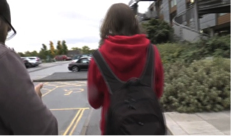
\includegraphics[width=0.5\textwidth]{img/study2/ep3/ep31}
\caption{episode 2.3, AW (right) leads the way, heading to target 44 as instructed.}
\label{fig:study2ep31}
\end{figure}

\begin{figure}[ht]
\centering
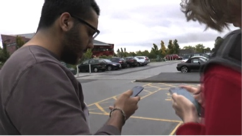
\includegraphics[width=0.5\textwidth]{img/study2/ep3/ep32}
\caption{episode 2.3, After the team received an instruction to disband, AW (right) and HB (left) simultanously turn back and start walking back to the drop off zone, displaying bodily alignment.}
\label{fig:study2ep32}

\end{figure}

\noindent\texttt{\textbf{Episode 2.3}\\
\emph{ [00:00] HB, AW at drop-off zone, new instruction received: AW, HB->44} \\
\textbf{HB:} Alright, who is AW? \\
\textbf{AW:} Me.\\
\textbf{HB:} let's go southeast (the direction of target 44).\\
\emph{[00:07] AW, HB looking at their screens.}\\
\textbf{[00:26] HB:} There is no 44.\\
\textbf{AW:} down there.\\
\textbf{HB:} Ok, yea, yea, yea (0.5), I can`t see, Oh, there, yea, let`s go.\\
\emph{[00:35] [Fig.4] Team begins moving towards 44.}\\
\emph{[00:48] HQ sent message: Target 42 and 44 is not reachable.} \\
\textbf{AW:} ((reads out the message))\\
\emph{AW and HB stopped walking.}\\
\emph{[00:52] New instructions received: AW, KD -> 44, HB, AR->31}\\
\textbf{AW:} I got a new instruction.\\
\emph{[Figure \ref{fig:study2ep31}] AW and HB simultaneously turn and start walking back towards the drop off zone.}\\
\textbf{HB:} I need to team up with AR.\\
\textbf{AW:} I need to team up with KD! Oh, it is 44 again.\\
\emph{ [01:01] AW, HB arrived at drop off zone, met AR, KD.} \\
\textbf{HB:} AR?\\
\textbf{KD:} AW? We have got (1.0), 44, right?\\
\textbf{AW:} It said 44 is not reachable, but I got it again, so, let`s try.\\
\textbf{KD:} Alright. \\
\emph{[01:14] AW, KD begin walking to 44, AR, HB team up as well.}\\
}



This episode begins with an instruction (AW, HB -> 44) from the agent. At that moment, there were 5 players at the drop off zone (AR, KD, LC, HB, AW). Immediately after the instruction, HB starts looking for AW in the local group. Shortly after, AR and HB team up to go for 44 as instructed.  However, 13 seconds later the team is interrupted with a HQ message telling them not to go for 44 (Target 42 and 44 is not reachable). Four seconds later, a conflicting agent instruction was delivered, implying they disband the team (AW, KD -> 44, HB, AR->31) but still pursue the target 44. At first, AW stops walking and topicalises the instruction (``I got a new instruction''), followed by both teammates simultaneously turning towards each other (Figure \ref{fig:study2ep31}, \ref{fig:study2ep32}). The bodily alignment in the action suggests agreement to follow the new instruction. On their way back to drop off zone, HB and AW confirm their intentions (``I need to team up with AR'', ``I need to team up with KD!''). In this case, the teammates respond to the interruption by mutually agreeing to abandon the current team and task in favour of following the new assignment. \\

It should be noted that the interruption was received only 17 seconds after the team commenced the task, probably contributing to a low perceived cost of abandoning the current task. Further, all players involved in the subsequent reteaming were not far away from each other. AW and HB had not walked far from the drop off zone; so everyone was still within line of sight, further facilitating successful reformation. \\

\subsection{Disagreement on task interruption}

\noindent\texttt{\textbf{Episode 2.4}\\
\emph{[Following on from Episode 2.3]}\\
\emph{AW, KD on their way to target 44.}\\
\emph{[01:39] New instruction received again, AW, HB -> 44, AR, KD ->31}\\
\textbf{AW:} new instruction, HB and 44 again, haha.\\
\emph{AW turns back towards drop off zone immediately.}\\
\textbf{KD:} AR and 31 ((Reading his new instruction)) ehh, have they gone? Because we can just decline and carry on.\\
\textbf{AW:} Ok, I rejected it. \\
\emph{AW turns back towards KD, who also rejects the new instruction. They resume their walk to 44.}\\
\emph{[01:54] New instruction delivered to AW (AW, YF ->46)}\\
\textbf{AW:} new instruction 46, yeah! ((team stop walking))\\
\textbf{KD:} Do they know we are already on the task?\\
\emph{[02:00] New instruction delivered to AW (AW, LC ->37)}\\
\textbf{AW:} yea, but I think, Oh, no, got new instruction again, (team up with) LC.\\
\emph{[02:13] AW starts walking to LC, who is at drop off zone within line of sight, leaving behind KD.}\\
\textbf{KD:} ((reads out HQ message)) AW and KD you won`t reach 44.  Alright, Let`s go to 46.\\
\emph{AW ((turning back towards KD)): I don`t know, I got a new task with LC.}\\
\textbf{KD:} Ahh, I do not have a task. \\
\emph{AW turns and walks towards LC again. KD follows.}\\
}


In this fragment, we can observe disagreement and negotiation of team reformation. Following episode 2.3, player AW disbands his team with HB and teams up with KD. However, 20 seconds after the reformation, AW is instructed to abandon the on-going task again. AW laughs, but turns back to find player HB again. Before AW sets off, KD disagrees with the new instruction and proposes to reject it (``Ehh, have they gone? Because we can just decline and carry on''). AW accepts KDs suggestion and turns back to KD.\\

After the rejection, AW receives 2 consecutive reteaming instructions from the agent, finally teaming them up with LC, while KD does not receive another instruction. KDs question (``Do they know we are already on the task?'') suggests that he might think the agent is unaware of their situation, and that he disagrees with disbanding the existing team. In spite of KDs disagreement, AW declares his intention to follow the new instruction (``got new instruction again, [team up with] LC'') and he turns to find LC. However, KD ignores this (``Alright, Lets go to 46''), indicating he does not agree with AWs intention to disband the team. AW interjects (``I dont know, I got a new task with LC''), and continues to walk towards LC, denying KD. As KD realizes he is without assignment (``Ah, I do not have a task''), he follows AW to find LC. \\

In this episode, teammates agree to reject the first task assignment. We found task interruption could be a major reason to reject new instructions. 10 out of 11 rejected instructions are associated with task interruption. In an extreme case (not pictured), one team reached an agreement to ignore any agent instructions after the agent tried to interrupt the teams` on-going task. \\

In the end, the player that received the new instruction disagrees with his teammates suggestion to ignore the instruction and decides to leave the current team. The team is disbanded in disagreement, in contrast to episode 2.3 where both teammates agree to leave the team after both received new instructions at the same time. Here, the teammates spend a fair amount of time arguing whether to follow or ignore instructions, hinting at the hidden social cost of agent coordination algorithms when applied to human teams. \\

Overall, the majority of new instructions that interrupted on-going tasks required team reformation. When tasks were interrupted, the rate of compliance (22 percent) is substantially lower than when teams were required to reform after a task was completed (50 percent). Task interruptions were also much more likely to lead to rejection of the new assignment: 10 out of 11 assignments that interrupted tasks were rejected.\\

\subsection{The headquarters}

HQ sent a total of 147 messages in the two sessions. We identified 50 assertives and 68 directives in two sessions through speech act analysis \ref{sec:aprmsg}. The majority of assertives were focused on providing situational awareness and safely routing the responders to avoid exposing them to radiation. E.g. ``NK and JL approach drop off 6 by navigating via 10 and 09.'' or ``Radiation cloud is at the east of the National College.''\\

16 out of 68 directives were directly related to task allocations and teaming, which is substantially less then the number of agent instructions (51). Among the 16 directives, HQ sent 11 direct instructions to the field players (e.g. ``SS and LT retrieve 09''), while the remaining 5 are related to forward planning, (e.g., ``DP and SS, as soon as you can head to 20 before the radiation cloud gets there first''). 6 of the HQ instructions are consistent with agent instruction, while 5 other HQ instructions override the agent instructions. It is worth mentioning that field players implemented only 5 out of 16 HQ instructions. In the interview, HQ reported that they felt they supported the agent rather than taking control. \\

%Insert a diagram here.

\section{Discussion}
In the previous sections, we described how the agent guidance is interleaved with social interaction, in which teammates organise the task planning and execution. We found that while the agent supported division of labour, the agent guidance had various social implications. We now reflect on (1) how division of labour is achieved; (2) the social implications and hidden cost incurred by team reformation and task interruption; and (3) the limited feedback mechanism. \\

\subsection{Division of labour between the agent and the human teams}
Overall, players followed 30 out of 51 agent instructions, out of which 21 tasks were completed according to the instruction (success rate of 70 percent). Only 2 targets were evacuated without agent instruction (Figure \ref{fig:study2agentInstructions}), which indicates that, to a large extent, the agent successfully supported routine task planning activities. Episode 2.1 demonstrates a typical case of division of labour: the agent handles planning of teaming and task assignment, freeing the team to focus on other issues such as navigation (identifying the target on the interactive map and finding directions) and organising team meet up.  The following of agent instructions speaks of players trust in the agents decisions. In the 30 cases where instructions were followed, we can observe similar patterns of division of labour.\\

The distribution of HQ messages may also indicate a division of labour between HQ and the agent. Only a small proportion (16 out of 147) is directly related to task assignment, indicating routine task allocations were delegated to the agent. A relatively large proportion (118 out of 147) of messages are used to provide situational awareness and safety routing the responders to avoid radiation exposure. However, the fact that only 5 (out of 16) HQ instructions are implemented suggests that HQ was unable to effectively override the agent when they wanted to. This fact highlights that the planning agent plays a strong role in the control loop, compared to the human coordinators in the HQ. The planning agent can directly instruct field responders without consent of the HQ, and the HQ does not have an effective way of overriding the agents decision. \\

\subsection{Hidden costs of team reformation and task interruption}\label{sec:study2social}
With this division of labour introduced in the previous section, it appears that system can successfully generate plans for humans to ``executes''. However, Following the view of situated actions \citep{Suchman1987}, The plan is actually a resource in the situation that human can leverage or not. In what follows, we reveal the significance of the plan in determining humans`s actions varies based on the social situations the players are in. 

First, while the compliance rate with agent instructions was high when no reteaming was required (91 percent), we found that the rate of compliance with agent instructions is much lower when team reformation is involved (50 percent), and even lower when in addition an on-going task is interrupted (22 percent) (Table \ref{tab:compliancerate}). Our interaction analysis shows the ways in which team reformation and task interruption are associated with hidden costs in the social organisation of team performance.  \\

\begin{table}[h]
\footnotesize
\begin{tabular}{l|ccc}
Context                   & \multicolumn{1}{l}{Instructions} & \multicolumn{1}{l}{Followed by FR} & \multicolumn{1}{l}{Compliance rate} \\ \hline
Instructing existing team & 23                               & 21                                 & 91\%                                \\
Require team reformation  & 10                               & 5                                  & 50\%                                \\
Interrupting tasks        & 18                               & 4                                  & 22\%                                \\
Total                     & 51                               & 30                                 & 59\%                               
\end{tabular}
\caption{Compliance with agent instructions by context}
\label{tab:compliancerate}
\end{table}

We found that team disbanding can be difficult. Players have to make their actions accountable to gracefully disengage from an existing team to avoid breaching social norms (e.g., politeness). Members have displayed a sense of attachment to a local group (episode 2.2), which delayed the task substantially until the team reformation failed. Despite interrupting an on-going task, new instructions for both teammates can facilitate smooth, mutually agreed disbanding (Episode 2.3), while instructions for only one member have coincided with interactional trouble, disagreement and delays (episode 2.4). \\

The impact of attachment between co-located teammates was further amplified by distance between proposed teammates. While they frequently accounted for actions with co-located players, they did not make their actions equally accountable to remote team members. For example in episode 2.4, the agent interrupted the local teams task and instructed them to team up with distant players. The co-located team decided to reject the instruction without contacting the potential teammates they rejected. The system lacked support for accountability between remote members. \\

A further observation is that players were unwilling to give up on-going tasks after a certain time. In episode 2.4, the teammates first agree to ignore new instructions. This preference to stick with on-going tasks may also explain the high rejection rate for instructions involving task interruptions. \\

The social organisation of coordination reveals implications for the simple model of interaction held by the agent. The agents algorithm re-plans and reshuffles teams, in order to optimise group performance by minimising the travel distance to the targets. However, the study has revealed the ways in which social norms and the accountability of social conduct get in the way. This raises questions about the effectiveness of approaches that treat coalition formation of humans as unproblematic. The agent does not consider the social cost of team reformation and task interruption.The study has shown that the social process to disengage from groups and on-going tasks can be costly. The tension between the social process and the model held by the agent echoes the notion of workflow from within and without \citep{Bowers1994}. The authors point out that models imposed by technology (from without) may come into tension with the actual workflow achieved through methods internal to the work (from within). 



\subsection{Feedback to the agent}\label{sec:studytwofeedback}

To recap, a feedback mechanism was included in the interaction design to give responders some control over the task assignment (Section \ref{sec:study2feedback}). On receiving an instruction, players can either accept or reject the instruction. On rejection of a task allocation, a new plan is requested. The rejected allocation is, in turn, used as a constraint within the optimisation run by the planning agent, which means that the rejected target will not be assigned to the rejecting player for a time (1 minute). \\

Our observations show there may be a significant cost associated with rejection. Overall, 6 out of 25 re-plans were triggered by rejections. In turn, tasks were re-assigned to all players (not just for the play who rejected). Frequent new instructions may cause extra coordination overhead (time spent on interpreting new instructions, more team reformation and task interruptions) and over-constrain the planning task. Players did not seem to be aware of the implications that their rejections had on others.\\
 
We also found that players` expectations of the rejection were not always aligned with its actual effect. Instructions involving reformation and interruption were more likely to be rejected. Players` statements indicated that they perceived the rejection as a way to reverse to previous states (Episode 2.4). Other statements indicated rejections were expected to pair them with a new teammate instead of a new target. The mismatch between expected and actual effect highlights a lack of intelligibility in the current interaction design. We aimed at simplicity (by providing only accept/reject options), which might be important for interaction in time-critical task settings, but it comes at the cost of intelligibility. Therefore, we argue that intelligibility and simplicity need to be carefully balanced according to details of the setting.\\


\section{Design implications}

Our observations reveal the tension between agent planning support and the social organisation of teamwork. The tension does not simply mean that the model held by the agent is incorrect; it highlights potential trade-offs we need to consider in system design \citep{Bowers1994,Sukthankar}. Providing a detailed design solution is beyond the scope of this thesis. Instead, we propose three design implications to scaffold the division of labour when building agent-based planning support for human teams.\\

\subsection{Achieve common ground}  
Two main issues arose that challenged the basis for collaboration \citep{Bradshaw2011}. Firstly, a notion of the social cost associated with instructing teams should be taken into account when designing planning agents. For example, disbanding teams can be difficult and time-consuming as it is governed by rules of social conduct and etiquette, particularly where the new teammates are out of sight or only one of the teammates receives a new instruction. Secondly, a mismatch between the expected and actual function of rejections further shows intelligibility needs to be improved. Therefore, we suggest that the design of agent support should a) takes social factors into consideration (e.g., ensuring team disbanding is facilitated by reteaming both teammates at the same time; avoiding task interruptions etc.), and that b) agent functionality is appropriately surfaced to help achieve common ground (e.g., by providing explanations of agent action at the interface level).

\subsection{Facilitate accountability}
While the rules of social conduct ensured accountability of action among co-located teammates, we found the impact of rejections on remote players was not properly appreciated; nor did the interaction design support making these rejections accountable. Therefore, we believe the interaction design should reveal the hidden cost of certain actions (e.g., rejections) to facilitate the accountability of local decision making accountable to remote team members, ensuring consequences of local decisions for the welfare of all teams are understood. 

\subsection{Balance responsibilities between humans and agent}\label{sec:balanceResponsibility}
 The social implications and other situational contingencies are likely difficult to be modelled computationally. Alternative approaches argue for mixed-initiative  control and flexible autonomy between humans and agents \citep{Bradshaw2011}. The ways in which the HQ used messsages to provide situational information that complemented the agent instructions show that humans are able to deal with arising situational contingencies. The division of labour between humans and the agent appeared generally effective in that the agent took on routine and repetitive jobs (task assignment), which freed the responders to focus on the situated rescue mission. In this on-the-loop interaction design, the role of the human HQ was relatively weak. For example, the HQ struggled to override the agents` instructions through the messaging channel. In the next study we explore an in-the-loop design which seeks to allow the HQ to play a stronger role in the control loop to enable more direct mediation and amendment of agent instructions (e.g., by directly modifying the task assignments, or by adding information relating to the assignments, such as safe routing).
 
%==== what is possible situational contingencies? social implications, coordination overhead incured is hard to be modelled, and other unexpected situational contingencies are hard to be considered by the agent. The example being some players is reluctant to disband team and unwilling to team up with remote players. As they are hard to be considered and model by the agent, HQ's input can be useful to judge the situation and contribute to the planning. In this field trial, The division of labour between humans and the agent appeared most effective in that the agent took on routine and repetitive jobs (task assignment), which freed the responders to focus on the situated rescue mission. However, the HQ is weak in terms of influencing the planning and plan executions. The reason has been summaried in section xxx. Here, we propose some requirements based on the.  ====%

\section{Summary}

In this chapter, we examined how the guidance from a planning agent is handled socially in the Human On-the-loop setting. To support our field trial we integrated a planner agent with AtomicOrchid and modified both mobile and HQ interface to facilitate the On-the-loop interaction pattern between human and agent. Findings from interaction analysis of field observations, triangulated with log files, reveal how the On-the-loop interactions played out. The results of the analysis show a division of labour in which the agent takes over the majority of planning activities while field responders only focus on other issues such as finding routes and targets. However, field observations also reveal significant costs associated with instructions that require members to reform new teams, and that interrupt on-going tasks. In addition, some confusions and misunderstanding are also discovered in the human agent feedback loop. Based on the findings, we presented three design implications to consider when creating agent-based planning support systems for human teams, including establishing `Common Ground', facilitating accountability and balancing responsibilities between human and agent.\\


%************************************************
\chapter{AtomicOrchid Study 3: Agent-supported In-the-loop design}\label{ch:studythree} 
%************************************************
This chapter presents the third iteration of the \acf{AO} field trials. The purpose of this iteration is to investigate socio-technical issues relating to agent planning support with a Human In-the-loop interaction design. Based on the On-the-loop version of AtomicOrchid (Section \ref{sec:studytwosystem}), the system has gone through another development iteration to facilitate an in-the-loop interaction pattern. Through interaction analysis of video recordings and game log data, we reveal how this In-the-loop design unfolds and, through a number of critical incidents, how it breaks down. A workshop with a professional disaster response team is conducted to reflect on realism of AtomicOrchid scenario. \\

%and raises the challenge to extend this work to more complex but slower paced situations.   \\

%We find that the human coordinator and automated planner agent can successfully work together in most cases, with human coordinators inspecting and `correcting' the agent-proposed plans. However, occasional failures of planning are also observed due to: complacency; silent, missing or invisible information; and limited support for human planning.

\section{Introduction}
%Most disaster operations require responder teams to plan and carry out task under spatial and time constraints. which means the teams often have limited resource and personnel to deal with large amount of geopolitically distributed tasks in limited amount of time. How do they optimise the use their rescue resources become computationally complicated problem. Multi-agent system researchers have developed a number of multi-agent task allocation algorithms. As software components, they have all done very well in the computational simulation, therefore there is potential to apply those algorithms to support planning activity of human responder teams. \\

%However, these algorithms necessarily depend on abstracted models of the environment and human behaviour which might lead to task allocations that are flawed in practice, due to the contingent nature of situated action \cite{Suchman1987}. 

In this study, we keep refine the \ac{AO} interface and place a human coordinator in-the-loop between the planning algorithm and the physical world. The in-the-loop design pattern assumes the constant HQ supervision and intervention is required to ensure the agent works properly (section \ref{sec:approachPatterns}). The AtomicOrchid system has evolved from the second game probe in study 2 (chapter \ref{ch:studytwo}), to facilitate the In-the-loop interaction. The In-the-loop design enables HQ human to involve in the planning process by: \\

%However, there is concern that the algorithms hold over-simplified model of the environment and human behaviours. Therefore, effective interactions with the responder teams may be required to ensure the planning agent actually support (rather than hinder) the planning process of responder teams, which highlights the importance of appropriate interaction design. 

\begin{enumerate}
	\item allowing HQ to review, edit and approve every instructions generated by agent. (Figure \ref{fig:study2InTheLoop} (1)). In extreme cases, HQ can override all agent instructions, i.e. manually allocate all tasks;
	\item allowing HQ to decide when to initiate re-planning (Figure \ref{fig:study2InTheLoop} (2)); and
	\item allowing HQ to review feedback from field players and decide how to act on them. (Figure \ref{fig:study2InTheLoop} (3))
\end{enumerate}

\begin{figure}[h]
  \centering
  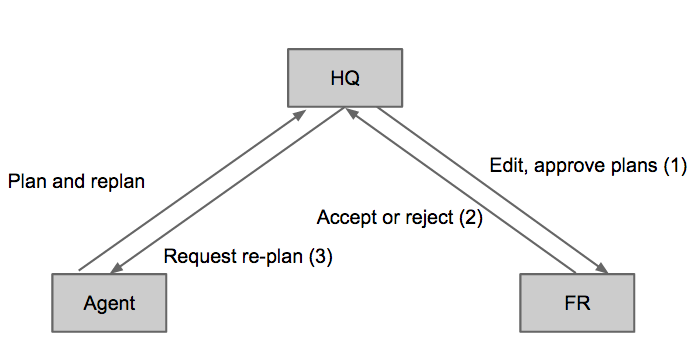
\includegraphics[width=1\textwidth]{img/study3/InTheLoop}
  \caption{In-the-loop interaction design}
  \label{fig:study2InTheLoop}
\end{figure}

Compared to the human on-the-loop design in the previous study (Section \ref{sec:approachPatterns}, chapter \ref{ch:studyone}) , the major change is the rebalancing of responsibilities in the control room (between HQ and agent). The interaction between field responder and the control room is mostly unchanged. Therefore, this study has a strong focus on control room interaction compared to study 2. More specifically, the objective of this study is to unpack the human agent interaction in the human In-the-loop paradigm, particularly in the control room, revealing division of labour, interactional issues and design implications that can be drawn from the interactions. Findings from the study reveal the processes in which the agent and HQ players collectively generate task assignments for field players. Occasional failures in the process highlights a set of issues including complacency; silent, missing or invisible information; and limited support for human planning. In addition, a workshop with a professional disaster response team is reported in this chapter to reflect on realism of AtomicOrchid scenario. \\


\section{System Evolution}\label{sec:study3system}
The in-the-loop version of AtomicOrchid is not designed from scratch, but evolved from the on-the-loop version introduced in previous study (Section \ref{sec:studytwosystem}). In study 2, we observed HQ struggling to get involved in the planning loop even when they wanted to intervene. Combining the observations from the study 2 and the definition of the in-the-loop interaction pattern (\ref{sec:approachPatterns}), we further generate several system requirements for realizing the In-the-loop interaction. \\
\begin{enumerate}
\item HQ should be able to review, edit and approve every instructions generated by the agent.
\item HQ should be able to decide when the agent should re-plan. 
\item HQ should be able plan for part of the team, leaving the agent to plan for the rest of the team. 
\item HQ should be able to communicate their assignments (or task cancellation) to FRs in a structured way. 
\end{enumerate}

The purpose of requirement 1-2 is to give HQ more control over the planning loop, by delegating to them the responsibility for final decision in planning. Requirement 3 enables HQ to modify the agent planning without having to take full manual control of plan generation. Requirement 4 is derived from the observations (study 1 and 2) that HQ struggled to override agent planning through unstructured text messages. Therefore, we suggest that HQ should be able to deliver and cancel their assignments in the same structured way that the agent do. Two interfaces are designed for the 2 HQ players in the control room. The task assignment interface provides a set of interface functionalities supporting task allocation activities, while the situational awareness interface provides game status and a broadcast message channel \ref{fig:study3messaging}.  \\

% the mobile responder app
\begin{figure}[h]
  \centering
  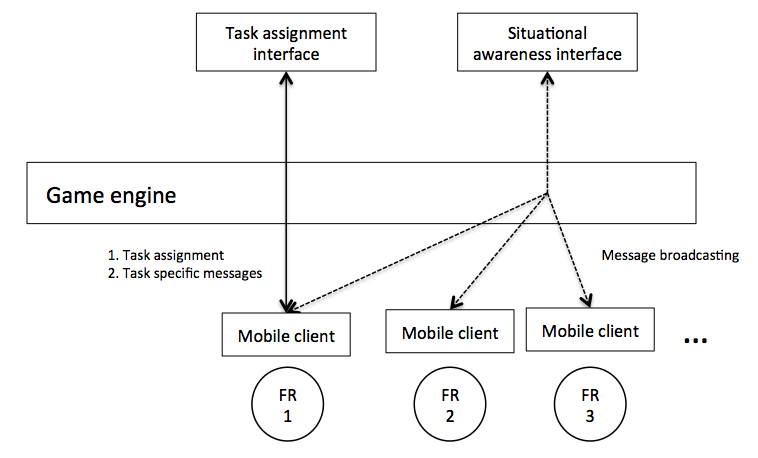
\includegraphics[width=1\textwidth]{img/study3/system/Interfaces}
  \caption{Messaging system design}
  \label{fig:study3messaging}
\end{figure}

%1. Plan request:  HQ can request planner to generate plan (at 1). Agent conducts task optimization based on current task status, and proposed on optimal plan to HQ for review.\\
%2. Plan review: HQ can choose make some minor edits to agent proposed plan. Alternatively, the HQ can propose some assignments, and re-initiate step (1) to let the agent conduct partial planning for the rest of the team (explain for partial planning, see section x). \\
%3. Plan approval: If HQ is satisfied with the plan, he/she can send the plan to field responders for execution. \\
%4. Feedback and further communication: When Field responders receive plans, they can communicate with HQ to provide feedbacks and request clarifications. Based on the task execution status and feedbacks, HQ can decide to initiate to step (1) again for re-planning. \\


\subsection{Interfaces}
This section describes the three game interfaces used by players, which are the mobile responder interface for field responders, the task assignment interface and the situational awareness interface for HQ players.\\

Compared to the on-the-loop version of AtomicOrchid, the mobile interface is largely unchanged except for the HQ task tab (Figure \ref{fig:study3mobileInterface}). The task tab now displays a task with text description and map visualisation of the task at the top. The bottom half of the interface is a message box showing task-specific information from HQ. It should be noted that the HQ can still send broadcast information (visible to everyone), which will be displayed in the chat tab. \\

\begin{figure}[h]
  \centering
  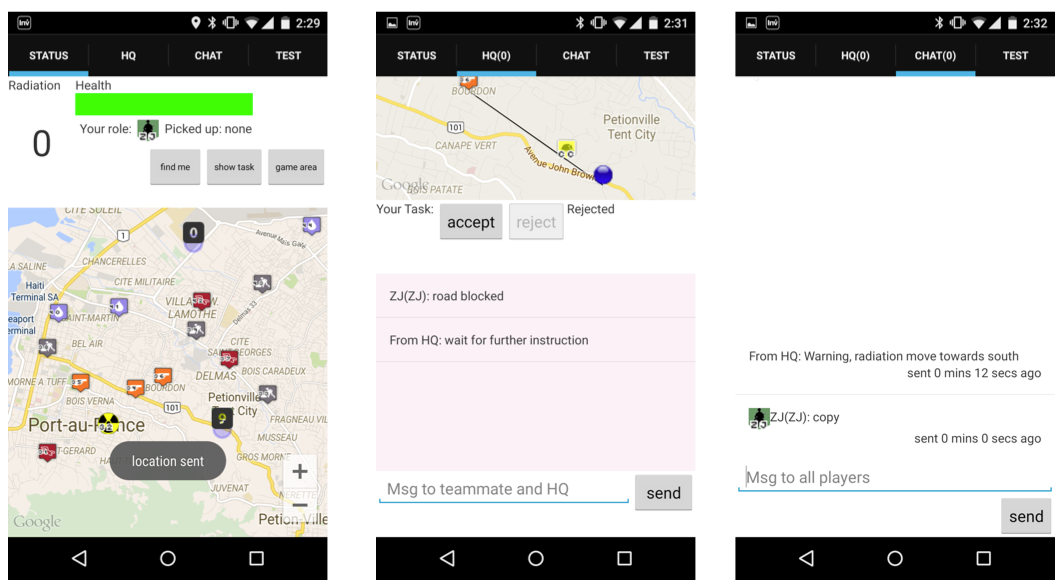
\includegraphics[width=1\textwidth]{img/study3/system/mobileInterface}
  \caption{Mobile interface in study 2}
  \label{fig:study3mobileInterface}
\end{figure}

The situational awareness interface is the same as the HQ interface used in study 2 (Section \ref{sec:studytwointerface}). It provides information about game status monitoring, and a broadcast message channel for communicating with field players(Figure \ref{fig:study3SAinterface}).\\

\begin{figure}[h]
  \centering
  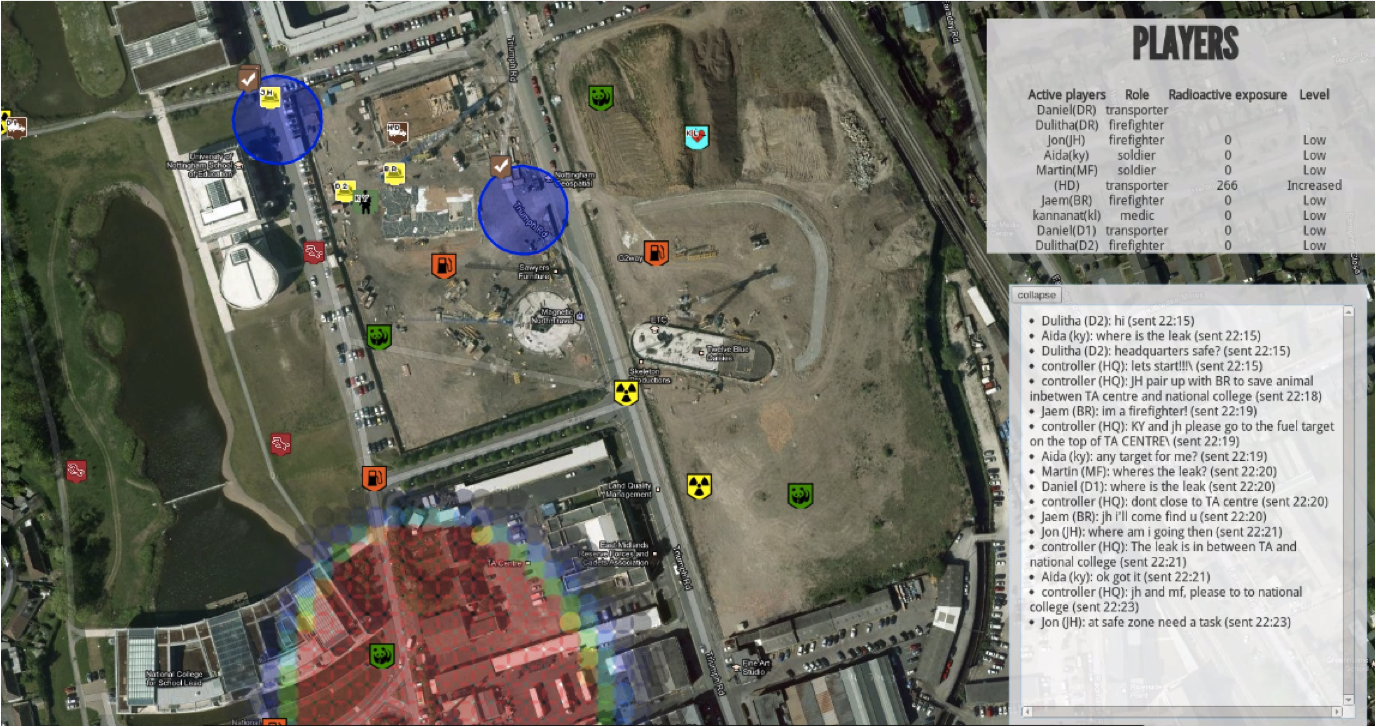
\includegraphics[width=1\textwidth]{img/study3/system/HQ2Interface}
  \caption{Situational awareness interface operated by HQ2}
  \label{fig:study3SAinterface}
\end{figure}

The task assignment interface is created to support In-the-loop interaction with Agent. As an overview, the interface has a map on the left. The figure \ref{fig:study3TAinterface} is a screenshot of task assignment interface. Components are numbered in the figure to illustrate functionalities of the interface. Player/target locations and assignments are presented on the map. At right side of the interface is a task assignment panel. The left (1) column of the panel shows pending assignments while right column (2) shows existing task status. Figure  \ref{fig:study3TAinterface} (5) shows an example of a proposed task assignment: player MD and GO are assigned to target 07. Within each confirmed task assignment (6) a feedback indicator indicates the field player`s response to this assignments (no response, reject, accept).\\

\begin{figure}[h]
  \centering
  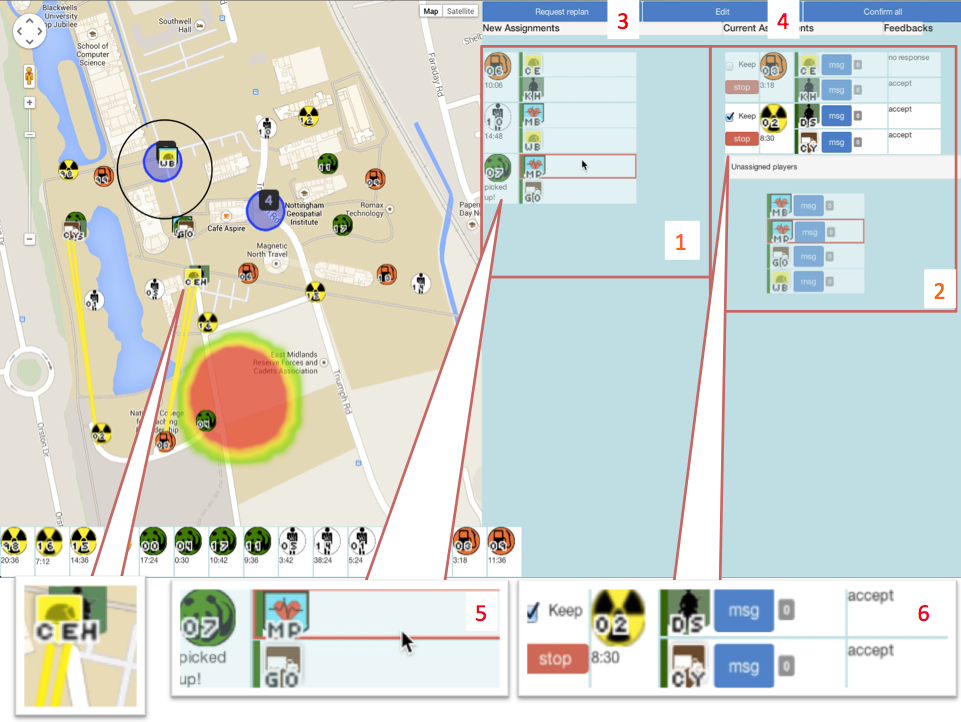
\includegraphics[width=1\textwidth]{img/study3/system/HQ1Interface}
  \caption{Interfaces in study 3}
  \label{fig:study3TAinterface}
\end{figure}

\begin{figure}[h]
  \centering
  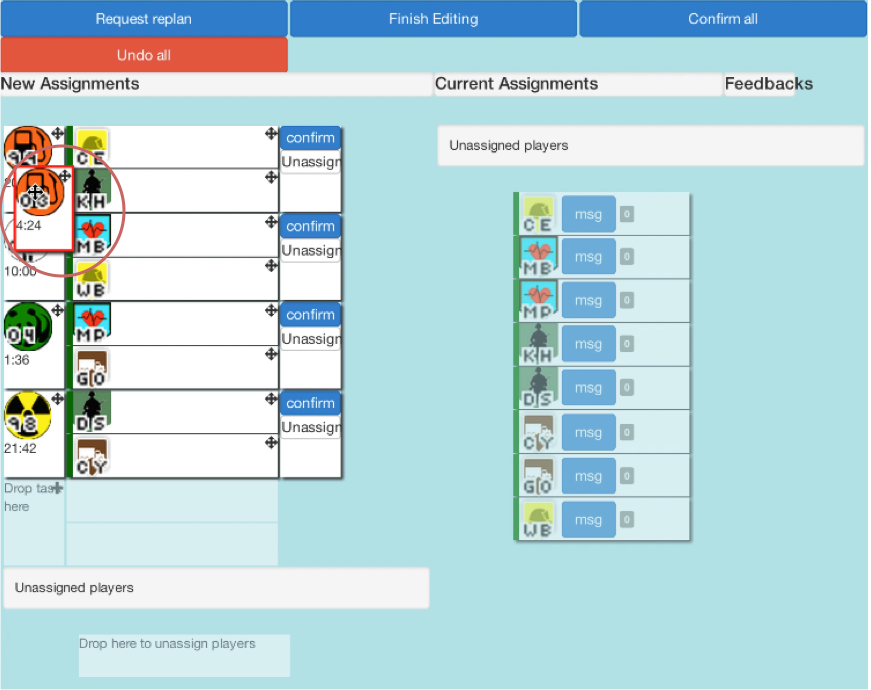
\includegraphics[width=0.5\textwidth]{img/study3/system/editmode}
  \caption{Edit mode of task allocation interface}
  \label{fig:study3editmode}
\end{figure}

\begin{figure}[h]
  \centering
  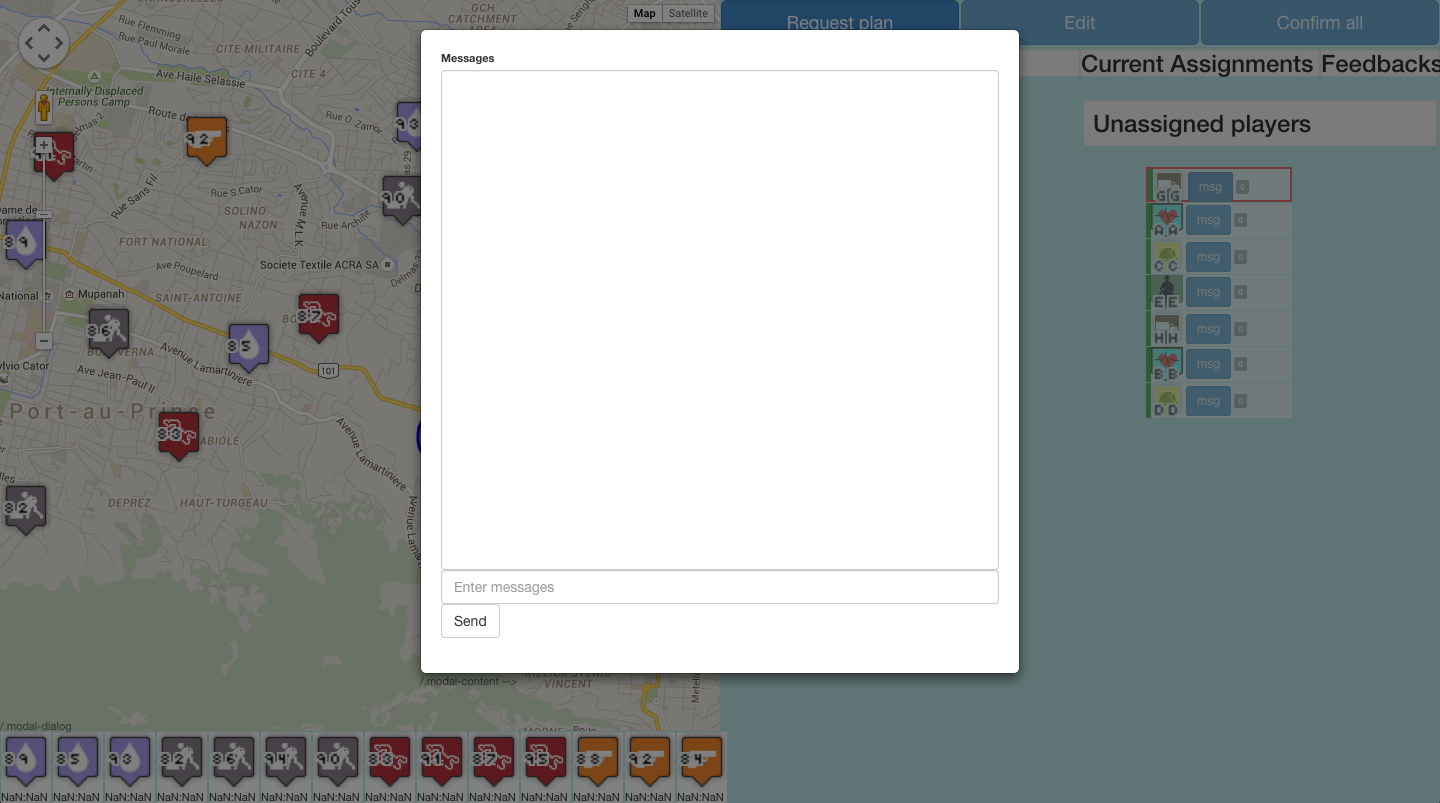
\includegraphics[width=1\textwidth]{img/study3/system/msgmode}
  \caption{Pop up messaging panel}
  \label{fig:study3msgmode}
\end{figure}


\begin{itemize}
\item Plan request button: \\
This button triggers agent re-planning (Figure \ref{fig:study3TAinterface} (3)). The agent will calculate an optimized plan based on task status, and present it to the HQ on the pending panel. This button allows HQ to decide when to initiate a re-plan. \\

\item Plan keeping checkbox:\\
These checkboxes are attached to every task assignments in the confirmed panel (Figure \ref{fig:study3TAinterface} (6)). If the checkbox is ticked, the planner will keep the corresponding assignment in the next re-planning. In other words, the planner will keep the assignment fixed, performing partial planning for the rest of the team. 

\item Plan edit panel: \\
Manual plan edits will be activated by clicking the `edit' button (Figure \ref{fig:study3TAinterface} (4)). The assignments in pending area will change to edit mode. Assignment can be created, modified and deleted through drag and drop interaction (Figure \ref{fig:study3editmode}). \\

\item Plan approval button: \\
This button approves all pending assignments (Figure \ref{fig:study3TAinterface} (7)). All pending assignments will move to the confirmed area. Alternatively, assignments can be approved individually by clicking individual confirm button on the pending assignment when the edit mode is activated. \\

\item Text messaging panel:\\
The messaging panel (Figure \ref{fig:study3msgmode}) can be toggled by clicking msg button on the confirmed assignments (Figure \ref{fig:study3TAinterface} (4)). The panel is supposed to be used for assignment-specific information. Therefore, the messages in this panel are only visible to the two involved players and HQ.\\

\item The Feedback indicator:\\
The feedback indicators are attached to the right hand side of the confirmed assignments (Figure  \ref{fig:study3TAinterface} (6)). The field players can easily provide feedback on their assignment through the mobile responder interface (introduced later). There are three possible values for the indicator (no response, reject, accept). Because rejections typically indicate issues that needs to be followed up by HQ, the rejection will be highlighted with red. \\

When both involved players both accept the assignment, the keep checkbox will be ticked automatically. This is a mechanism to avoid accidental interruption of the accepted assignments in subsequent re-plans. \\

\item Stop button: \\
The stop button can be used to indicate an emergency termination of an assignment (Figure\ref{fig:study3TAinterface} (6)). If this button is clicked, the assignment will be dismissed both in the mobile and HQ interface. \\
\end{itemize}

%more images


\subsection{The planning agent}\label{sec:studytwoagent}

One big change to the planner compared to study 2 is the addition of a partial planning feature. The agent can take a list of fixed assignment as input. It then plan for the players and targets that are not involved in the fixed assignment list. This functionality has two potential uses: \\

\begin{enumerate}
	\item It allows human operators to contribute part of a plan and ask the agent optimize the rest.\\
	\item It allows human operators to annotate some on-going tasks, so that they could not be changed in dynamic re-planning. \\
\end{enumerate}

Apart from the partial planning feature, the input/output of agent is not changed.\\

%insert a summary picture.\\

\section{Study Design}
Participants were recruited through posters and emails. A total of 20 participants were recruited. 10 participated in session A and 10 in session B (Appendix \ref{app:demo3}). All participants were reimbursed with 15 pounds for 1.5 hours of study. For each game session, there are 2 HQ players and 8 field players. The majority of participants were students of the local university. The HQ players were recruited from researchers in the computer science department. \\

Because the HQ interface is a lot more complicated then that of the study 1 and study 2, we add an extra 0.5 hour training session before the formal study for HQ players to get familiar with the new task assignment interface. We anticipated that the workload of operating the human in-the-loop interface would be a lot more than that of operating the on-the-loop interface. Therefore, there are two HQ payers recruited in each session to split work in the control room. One of the two HQ player operates the new task allocation interface (described in section \ref{sec:study3system}), while the other player operates the situational awareness interface (described in study 2, section \ref{sec:studytwointerface}) to assist the other HQ player by providing situation awareness and sending broadcasting information. \\

Upon arrival in the HQ (set up in a meeting room at the local university), participants were briefed and asked to consent to participate. Roles were randomly assigned to field players (firefighter, medic, transporter, soldier). Field responders were provided with a smartphone; HQ coordinators with a laptop. Game rules and interfaces were introduced, and participants were assisted in setting up their phones and laptop clients. Field responders and HQ coordinators were given 5 minutes to discuss a common game strategy. All field responders were accompanied to the starting point within the designated game area, about 1 minute walk from headquarters.\\

Before the formal session begins, there was a training session for field players to get familiar with the mobile interface. The training session has a very simple game setting with only four targets nearby the starting point. The training session ends when field responders collect all four targets nearby. Once field responders were ready to start formal session, one researcher started the game engine, triggering a ``game start'' message to be sent to the mobile interfaces. Gameplay commenced for 30 minutes. A ``Game over'' message by HQ concluded the game. Field responders returned to HQ for the post-game session.\\

The game area was the same as for study 1 and 2, on the local university campus (Appendix \ref{app:area3}), 400 by 400 meters, without heavy traffic. The terrain of the game area includes grassland, a lake, buildings, roads, and footpaths and lawns. There are two drop off zones. Due to extra HQ training sessions and improved interface, the number of targets is increased to 20 (from 16 in study 2) to the increase game challenge.  There were four targets for each of the four target types. The pattern of cloud movement and expansion was the same for both game sessions and the same as for study 1 and 2.\\

We recorded both system logs and video of interaction in the field for analysis. To capture the distributed, concurrent nature of the interaction, four researchers with camcorders shadowed the field player teams, and one researcher recorded the action in the HQ. The replay tool was used to synchronise and analyse triangulated game events, player positions, and concurrent video recordings  (Appendix \ref{app:vis3}).\\

Our interest in this chapter is how socio-technical interaction is organised around the computational planning support, hence our focus is on the control room first, but then we trace information flow and decision making into the field. In practice, video recordings of the control room were catalogued to identify key decision points in teaming and task allocation, which served to index sequences (episodes) of interest (Section \ref{sec:aprIA}). Interesting distinct units of interaction were then transcribed and triangulated with log files and field video for deeper analysis; the results of which we present in this chapter.\\


\section{Data Analysis}
This section starts with overview of game results, messaging system usage and task assignments, as they served to index episodes of interest. Selected episodes of game play are then presented in order to unpack the interactions surrounding the task assignment activities in the control room. We provide these episodes as vivid exhibits of how members accountably organise their team coordination in situ \citep{Crabtree2012}. The order in which we present the episodes follows the common practice of moving from exhibits of typical/unproblematic instances, via more complex/difficult in- stances, to exhibits that display problematic interaction or even complete breakdowns (\citep{Heath2010}).\\

Overall, 28 of the 40 targets were evacuated in two sessions (16 in Session A and 12 in Session B). The player`s health status in session 1 is better  (Avg 90, Sd 9.3 ) then that in session 2 (Avg 48, Sd 41). Two deaths occurred at the begging of session 2. More details of death will be presented as episodes later in this section. \\

\begin{table}[h]
\centering
\footnotesize
\label{my-label}
\begin{tabular}{c|cccccc}
          & Target saved & Health max & Health min & Health avg & Health Sd & Death \\ \hline
Session A & 16           & 99         & 75         & 90.75      & 9.337     & 0     \\
Session B & 12           & 97         & 0          & 48.12      & 41        & 2    
\end{tabular}
\caption{Result overview of study 3}
\label{tab:ResultsOverview}
\end{table}

\subsection{Messaging system}
One change of the messaging system made for this iteration is separating channels for assignment-specific and broadcast messages. The HQ1, with the task assignment interface, is responsible for sending message in assignment-specific channel, while the HQ2, with the situation awareness interface, is responsible for sending messages in the general message channel. This section will reveal how this design plays out in the field trials. \\


\begin{table}[h]
\centering
\footnotesize
\begin{tabular}{c|ccc}
Session 1               & Sent by HQ & Sent by FR & Total \\ \hline
Broadcasting msg        & 35         & 3          & 38    \\
Assignment specific msg & 22         & 15         & 37    \\
Total                   & 57         & 18         & 75    \\
Session 2               & Sent by HQ & Sent by FR & Total \\ \hline
Broadcasting msg        & 31         & 13         & 44    \\
Assignment specific msg & 19         & 11         & 30    \\
Total                   & 50         & 24         & 74   
\end{tabular}
\caption{Task assignment overview}
\label{tab:ResultsOverview}
\end{table}

We found HQ  players frequently send messages to update FRs about the locations of the radiation cloud, (e.g. ``Radiation Status- 38  39  37 and Drop Point 7 all out of bounds'' ) and provide navigational guidance (e.g. ``go north  and west around the water''). HQ is also observed to send messages to repeat and enhance the task assignment (e.g. ``turn to 49'').\\

On the other side of the message channel, field responders send messages to request tasks (e.g. ``please advise'') and cloud status (e.g. ``Which way is it moving?''). Field responders also occasionally send acknowledgments to HQ`s messages (e.g. ``Copy that.''). \\

Most messages in the general message channel are general information about the clouds. However, we also found 11 messages in the general message channel (out of 82) are clearly addressed to individual teams. The specific player initials are mentioned in those messages. (E.g. ``NG and YI approach quicker to 41 drop off to 8'')\\

\subsection{Overview of task assignments}
In the following tree diagrams, plans are broken down into individual task assignments. Each individual assignment may go through 4 stages in the planning process (creation, approval, feedback, and execution). The assignment status for each stage is summarized in the following diagrams(Figure \ref{fig:TaskAsSession1},\ref{fig:TaskAsSession2} ). \\

\begin{figure}[ht]
 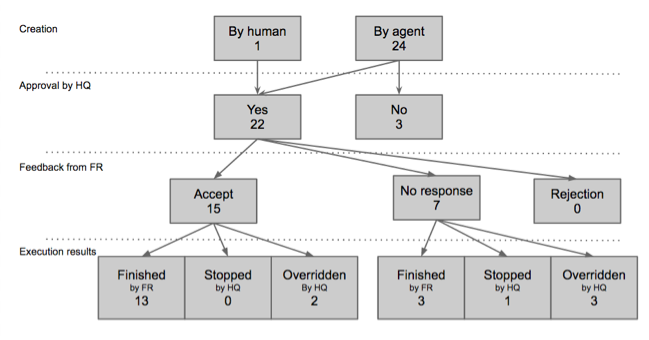
\includegraphics[width=1\textwidth]{img/study3/TaskAsSession1}
\caption{Task assignment in session 1}
\label{fig:TaskAsSession1}
\end{figure}

\begin{figure}[ht]
 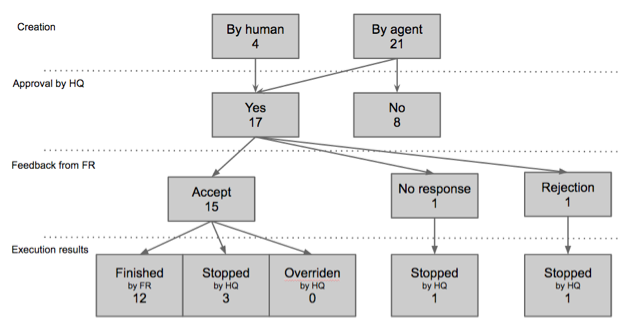
\includegraphics[width=1\textwidth]{img/study3/TaskAsSession2}
\caption{Task assignment in session 2}
\label{fig:TaskAsSession2}
\end{figure}

In summary, HQ and the planning agent contribute to the task planning activities in the control room. The planning agent created a total of 45 task assignments with an additional 5 assignments created manually by HQ. HQ approved a total of 39 assignments. Field responders accepted most of the approved assignments (30 out of 39). 9 assignments were rejected or not responded to. During task execution, occasional HQ interventions resulted in 5 task cancellations and 5 assignments being override. In the end, players managed to evacuate a total of 28 (out of 40) targets in 2 sessions.\\ 

Although the diagrams (figure \ref{fig:TaskAsSession1}, \ref{fig:TaskAsSession2}) suggest a sequential planning-execution process (creation -> approval -> feedback -> execution), we actually found that various planning activities (e.g. assignment creation, approval, intervention, communication) are highly intertwined in the control room setting. In the rest of the section, episodes of game play will be used to unpack the interactions surrounding the task assignment activities in the control room. The episodes in later sections will be presented with a standard orthographic notation detailed in section \ref{sec:aprIA}.\\

\subsection{Confirming the plan}
As summarised above, a majority of task assignments are generated by the planning agent and approved by the HQ players. The episode 3.1 demonstrates a typical case of the routine task planning process in control room. \\

\noindent\texttt{\textbf{Episode 3.1}
\emph{Context: HQ paid attention to a team (MV XW) who was carrying target 43 back to drop off zone 7.}\\
\textbf{16:45, HQ2:} XW and MV.\\
\textbf{16:50, HQ1:} (taking) 43. \\
\textbf{16:51, HQ2:} They should be going to drop off (zone) 7 and get 36 (Figure \ref{fig:study1ep311}) \\
\textbf{16:58, HQ1:} why don`t they go this way?\\
\textbf{16:49, HQ2:} tell them to go 36 afterwards.\\
\textbf{17:04, HQ1:} ok this one (refer to target 36). Do you tell them? (Figure \ref{fig:study1ep312})\\
\textbf{17:05, HQ2:} Should I tell them? (Typing)\\
\textbf{17:07, HQ1:} Yeah, go for 36. Maybe After the drop off, I think then (will) get confused.\\
\textbf{17:13, HQ2:} I will tell them to go after drop off.\\
\textbf{17:14, HQ1:} Yeah, Yeah. \\
\textbf{18.10,} (The team dropped off target 43)\\
\textbf{18:22, HQ1:} (click re-plan) \\
\textbf{18:26,} (new assignments, the team is assigned to MV,XW -> 36)\\
\textbf{18.28, HQ1} 36, yes (Click confirm)\\
}

\begin{figure}[ht]
\centering
\begin{minipage}[b]{0.45\linewidth}
\includegraphics[width=1\textwidth]{img/study3/ep11}
\caption{ep 3.1, HQ1 (left) HQ2 (right) }
\label{fig:study1ep311}
\end{minipage}
\quad
\begin{minipage}[b]{0.45\linewidth}
 \includegraphics[width=1\textwidth]{img/study3/ep12}
\caption{ep 3.2, HQ1 (left) HQ2 (right)}
\label{fig:study1ep312}
\end{minipage}
\end{figure}

At the beginning of this episode, the team MV, XW are carrying a target (43), approaching drop off zone. At [16:45], the HQ2 noticed the team was going complete its current task and began to consider a new target for them [16.51]. HQ2 proposes that 36 should be prioritized (Figure \ref{fig:study1ep311}). HQ1 agreed with the suggestion and decided to send the assignment after the team completes existing task (Figure \ref{fig:study1ep312}) [17:07]. At 18:10, the team dropped off target. After the drop-off, the HQ requested a re-plan. The agent assigns the team MV, XW to target 36, which is consistent with decision of the HQ players. At the end, HQ approved the assignment [18:28]. In this typical case of task assignment, HQ  can be seen to be monitoring the task execution, and making timely requests for new task assignments. HQ`s discussion suggested that the agent task assignment was approved after a careful review of player, target and radiation status. In addition, much of HQ1 and HQ2`s discussion happens before the team drops off the target; this kind of forward planning was observed on several occasions.\\

\subsection{Just Following the Plan}\label{sec:study3planfollow}
Episode 3.2 gives a more problematic example of accepting the planning agent`s task assignments. Episode 3.2-1 describes the interaction in the control room; while episode 3.2-2 gives the perspective of the field players.\\

\noindent\texttt{\textbf{08:32, Episode 3.2-1}\\
\emph{NG and YI have just completed a task together; DI is some distance away.}\\
\textbf{08:32,} (HQ1 request assignment for Idle player NG, YI))\\
\textbf{08:37,} (New assignment NG, YI -> 50) \\
\textbf{08:40,} (HQ1 confirmed plan) \\
\textbf{09:09,} (HQ1 request assignment for DI who has just become idle) \\
\emph{(NG have not confirmed the previous assignment; DI is closer to target 50)}\\
\textbf{09:16,} (New assignment arrived NG, DI -> 50 )\\
\textbf{09:17,} (HQ1 confirm NG, DI -> 50)\\
}



In this episode, the HQ1 requests assignment twice for idle players, which is a routine activity for HQ1 (As discussed in episode 1). Firstly, HQ1 request and approve new assignment for NG, YI [08:32]. 30 seconds later, DI become idle [09:09], so HQ1 request plan again. Because DI is closer to target 50 and NG YI have not accepted their assignment, the agent replaces DI with NG in the new assignment to minimize travelling distance of field players. Although HQ1 does not verbalize his reasoning process the quick approval suggests HQ1 may not have inspected the new assignment carefully and may not have noticed that the previous assignment will be overridden, potentially interrupting a task in progress. The episode 3.2-2 picks up the activity of NG and YI as the first new task assignment is approved by HQ.\\

\noindent\texttt{\textbf{Episode 3.2-2}\\
\emph{NG YI received a task update after they finished their previous task}\\
\emph{(Team NG YI received new task NG, YI -> 50)}\\
\textbf{08:39, NG: } Task changed, to what? \\
\textbf{08.43, NG: } Oh sh*t, there is a radiation zone sh*t. \\
\textbf{08:53, NG: } It (target 50) is close to the lake. It is triumph road we have to go that way. \\
\textbf{08:55, YI: } Yea, we need to. No this is the lake. \\
\textbf{09:00, NG: } Oh that is the river, so it is that way, Can we go? Yes we can go, this road?\\
\textbf{09:10, YI: } Yes it should be. \\
\emph{(Their task is interrupted by new assignment YI, DI -> 50)}
\textbf{09:18, YI: } Task changed.\\
\textbf{09:19, NG: } Task changed? What? \\
\textbf{09:23, YI: } No, it is the same.  \\
\textbf{09:26, NG: } I do not see anything. \\
\textbf{09:28, YI: } You are DI, right?\\
\textbf{09:29, NG: } No.\\
\textbf{09:30, YI: } En? You are no DI? DI, wait. \\
\textbf{09:37, NG: } I can not see my Task.\\
\textbf{09:45, YI: } You are NG, Oh no, I need DI.  \\
\textbf{09:48, NG: } You should go back then. Or send a message, Oh I can not see my task.\\
\textbf{10:02, NG: } I think the page is not loading.\\
}
 
NG and YI have already received the task to rescue target 50 but have not accepted or rejected it. While they are discussing how to reach the target the second task assignment arrives [09:10], the agent requires YI to team up with the remote player DI to pursue the same target, 50. The team is confused after the change of task. YI thinks that the task did not change because the target is still 50 [09:23] (YI: ``No, it is the same.''), and NG thought the interface is no longer working [10:02](NG: ``I think the page is not loading.''). After YI confirms NG`s initials, she realized she needs to switch teammate (to DI). \\

Overall, the task interrupt is resulted in a problematic sense making process in the field. Meanwhile the players in the control room appear unaware that anything untoward has occurred. The observation also reveals that several factors could have led to the task interruption including the absence of response from field responders; computational planning performed by agent without timely field feedback; and HQ`s failure to discover the task interruption during assignment approval. 

%This episode can be an example showing that computationally `optimized' assignment is not socially optimized for teams and HQ supervision failed to tackle the issue.\\

\subsection{Correcting the plan}
HQ players occasionally chose to change the task assign- ments generated by the planning agent; episode 3.3 presents one such example.\\

\noindent\texttt{\textbf{Episode 3.3}\\
\emph{CE and KH are currently assigned target 03 but have not accepted; other players are free}
\textbf{04:18,} (HQ1 click request plan)\\
\emph{(Assignments arrived: CE KH -> 06, MP GO ->07, MB ,WB -> 10)}\\
\textbf{04:24, HQ1:}  What? Why I am getting? Ahh, one of these guys does not accept. (Figure \ref{fig:study3ep31}) \\
\emph{(Referring to the team of CE, KH.)}\\
\textbf{04:29,} (HQ1 clicked keep on assignment CE KH -> 03) \\
\textbf{04:33,} (HQ1 request re-plan)\\
\textbf{04:40,} (Assignment arrived: MB, WB -> 10, MP, GO -> 07)\\
\textbf{04:42,} (HQ1 click confirm)\\
\textbf{04:56,} (MP, GO accepted)\\
}

\begin{figure}[ht]
\centering
\begin{minipage}[b]{0.45\linewidth}
\includegraphics[width=1\textwidth]{img/study3/ep31}


\end{minipage}
\quad
\begin{minipage}[b]{0.45\linewidth}
 \includegraphics[width=1\textwidth]{img/study3/ep32}
\end{minipage}
\label{fig:study3ep31}
\caption{ep 3.3, HQ identifies a task interruption, highlighted on right figure}
\end{figure}

After HQ requests a new plan, the agent proposes a set of assignments, one of which (CE KH -> 06) interrupts the existing task of a team (CE KH -> 03). HQ1 queries this change (``What? Why I am getting?'') realises that they have not explicitly accepted the previous task [04:24]. It should be noted that this kind of task interruption only happens when field players did not accept the tasks (Section \ref{sec:study3system}), making the agent think they are idle at that moment. After finding this problem, HQ then requires the agent to ``keep'' existing assignment [04:29] and requests a new plan from the agent, which is then approved. In contrast to episode 3.2, HQ1 notices and compensates for the field players` failure to explicitly accept the task, and the field players are able to continue with the previously allocated task without interruption.\\
\subsection{Changing the plan}
At the start of session B there is an extreme example of the HQ players overriding the planning agent. \\

\noindent\texttt{\textbf{Episode 3.4}\\
\emph{Context: At start of the session 1, all players were idle waiting for initial plan.}\\
\textbf{01:25,} (HQ1 requested initial plan)\\
\textbf{01:28,} (4 initial assignments arrived)  \\
\textbf{01:29, HQ1:}  why, it is stupid. \\
\textbf{01:33,} (HQ1 click edit)\\
\textbf{01:53, HQ1:} I want this one (HQ1 drag targets to replace agent planning) this one and this one.\\
\emph{HQ1 replaced 3 out of 4 targets in the task assignment. The three prioritized targets very are close to the original cloud}\\
\textbf{02:03,} (HQ1 clicked confirm) \\
\textbf{02:07, (HQ1 talk to HQ2) HQ1:} I think we should get the far ones first. \\
}

The episode begins with HQ requesting initial task assignments for the whole team. When the agent gives HQ  a set task assignments for approval, HQ complained about it [01:29, HQ: why, it is stupid.], indicating he is not satisfied with the plan. HQ then click edit button to switch to edit mode. Under the edit mode, HQ dragged 3 targets to replace the targets in agent assignments. The three prioritized targets are the ones that are closet to the radiation cloud. After HQ confirmed his modification [02:03], he said to HQ2 that the far away targets should be rescued first [02:07]. The execution result of this heavily edited plan is not ideal. Among the 3 three modified assignments, 1 of them is finished successfully, 1 assignment is cancelled later, and 1 assignment leads to player ``death''.\\

\subsection{Coping with the unexpected}
Episode 3.5 picks up shortly after episode 3.4, and exemplifies how HQ adapts task assignments to changing task status. \\

\noindent\texttt{\textbf{Episoe 3.5}
\emph{Context: after plans are confirmed in episode 3.4, HQs are monitoring FR's progress}\\
\textbf{02:09, HQ2:} they cannot walk there straight. (Figure \ref{fig:study3ep51})\\
\emph{Referring to team MB, GO, HQ2 point out that the straight path to one of the target is blocked by radiation}\\
\textbf{02:14, HQ1:} So who is that. (Target) 04 (HQ1 open the message panel) \\
\textbf{02:20, (HQ 1 Types message)}  You are heading to an area affected by cloud, You need to be very fast. [Fig 6] \\
\textbf{02:45, HQ2:} 04 is now in the cloud. \\
\textbf{02:45, HQ2:} Oh god, that is so fast.\\
\textbf{03:20, (HQ1 Types message)} Stay to the lake as possible!\\
\textbf{03:33, HQ1:} Shall we cancel (assignment 04) that or shall we wait for report? (HQ1 opens msg panel to talk to MP GO)\\
\textbf{03:43,} (HQ1 opens msg panel to talk to MP GO) \\
\textbf{03:50, HQ2:} I think (Target) 04 is only an animal, screw the animal.  \\
\textbf{03:52, (HQ1 Types message)} Abort, target compromised, proceed to target 07. \\
\textbf{04:06, } (HQ1 sent message)\\
\textbf{04:11, } (HQ1 click stop on the assignment of MB, GO->04)\\
}

\begin{figure}[ht] \label{fig:study3ep52}
\centering
\begin{minipage}[b]{0.45\linewidth}
\includegraphics[width=1\textwidth]{img/study3/ep51}
\caption{ep 3.5, HQ2 points to a team}
\label{fig:study3ep51}
\end{minipage}
\quad
\begin{minipage}[b]{0.45\linewidth}
 \includegraphics[width=1\textwidth]{img/study3/ep52}
\caption{ep 3.5, HQ sends msg for task cancellation}
\label{fig:study1ep52}
\end{minipage}
\end{figure}

After confirming assignments in episode 3.1, the HQ2 points out that one assignment may now be impractical because the route to target has already been blocked by a radiation cloud [02:09] (Figure \ref{fig:study3ep51}). HQ1 immediately opens message panel to send warnings and urge the team to move quickly (Figure \ref{fig:study3ep52}). However the cloud expansion seems to be faster then HQ originally expected [02:51]. Apart from sending route guidance to the team, HQ1 starts to consider cancellation of the assignment. After HQ2 agree with the cancellation, HQ1 sends a message to the team to inform them that the assignment is going to be cancelled and instructs them to go to new target 07. The assignment is formally cancelled in [04:11]. After HQ1 cancels the task, he starts to request new assignments from planner and allocates target 07 to the team later. In this case the HQ players realise the risk and are able to abort the task and redirect these field players out of danger.\\

\subsection{When it all Breaks Down} \label{sec:playerDeath}
In episode 3.4, in which the HQ modified 3 agent assignments. In the modified plan, the team CE, KM is instructed to go for a target very close to a radiation cloud. We look first at the HQ perspective (episode 3.6-1), and then at the field players` perspective (episode 3.6-2).\\

\noindent\texttt{\textbf{Episode 3.6-1}\\
\emph{(Context: One team (CE, KM) is end up heading to radiation cloud.)}\\
\textbf{4:52, HQ2 } They (CE KM) are walking right into their death. \\
\emph{(CE and KM were heading to target 03 which is now at opposite side of a radiation cloud)}\\
\textbf{5:14, (HQ messaging) } Careful, you are approaching the cloud. Move extremely fast to the cloud. Go around the lake to return.\\
\textbf{5:32, HQ: } God, too slow.\\
\emph{(The team CE KM is completely in the mid of radiation)}\\
\textbf{5.46, (HQ typing message) } Move closer to the lake.\\
\textbf{5:50, } (The team went through the cloud, their health is below 20, the target 03 is now at the edge of the cloud)\\
\textbf{6.39, HQ2: } What are they trying to pick up?\\
\textbf{6:43, HQ1: } The fuel.\\
\textbf{6.48, HQ2: } I am not sure whether they can survive picking up the fuel. No, now is more concern of surviving. \\
\textbf{7:05, (HQ messaging) } Abort 03, return top to (target) 99. \\
\textbf{9.04, } (HQ1 stopped task of CE KM) \\
\textbf{9.05-10:08, } (HQ requested re-plan 4 times, no new plan available for CE KM) \\
\textbf{9.50, HQ1: } No targets for them? There are lots of them. \\
(Team CE, KM stay in the cloud all the time, and finally dead)\\
}

At the beginning of the task, the radiation cloud is already between target and the field team CE and KM. The cloud is expanding quickly, which catches the HQ1 by surprise. As a result, 2 messages are sent by HQ1 to guide the team to avoid the cloud [05:14,5:46]. However the team is still excessively exposed to the radiation when they reach the side of the target, so HQ1 decides to abort the task [07:05]. After HQ1 cancels the assignment, the team is still exposed to radiation. HQ1 then tries to assign the players to other targets by requesting the agent for new assignments [09:05-10:08]. However, the agent does not assign the team to any task because the team`s health is too low. HQ1 seems to be confused about why the agent refused to assign targets. He repeatedly requests plans three times and says ``No targets for them? There are lots of them (refer to targets).''[9:50]. During this process, the team are still standing in the cloud. They finally lose all their health points and become incapacitated. Field players` perspective is given below. \\


\noindent\texttt{\textbf{Episode 3.6-2}\\
\emph{CE and KM are heading towards target 03}\\
\textbf{05:15, CE: } (Reading out the message) You are approaching the cloud, move extremely fast to the cloud, Ok! \\
\textbf{05:21,} (CE grabbed KM and started running) (Figure \ref{fig:ep361})\\
\textbf{06:12,} (The team CW, KM ran all the way across the cloud) \\
\emph{(After ran through the cloud, they are checking the health value.)}\\
\textbf{07:02, CE: } how dead are you?\\
\textbf{07:04, KM: } Pretty much dead.\\
\textbf{07:06, CE: } I am pretty dead as well.\\
\emph{(The team is trying to locate the target, but it is unsuccessful) (Figure \ref{fig:ep362})}\\
\textbf{07:28, CE: } Do you know what is funny? We have to get back.\\
\textbf{08:24, CE: } It should be somewhere around here! We are getting close.\\
\emph{(Assignment cancelled)}\\
\textbf{08:52, CE: } there is a new task, No task at the moment? \\
\textbf{[...]} 
\emph{(After assignment was cancelled, the team was still trying to locate the target)}\\
\textbf{09:44, CE: } I am pretty much dead and radiation is 12. Where is it! It says it is on this street but it is not. \\
\textbf{10:06, CE: } Oh I am dead.\\
}

\begin{figure}[h]
\centering

\includegraphics[width=0.7\textwidth]{img/study3/ep361}
\caption{ep 3.6, CE (left) grabs KM (right), start running into cloud. }
\label{fig:ep361}
\end{figure}

\begin{figure}[h]
\centering
 \includegraphics[width=0.7\textwidth]{img/study3/ep362}
\caption{ep 3.6, CE (left) grabs KM (right) walks around, looking into mobile screen, trying to locate target}
\label{fig:ep362}

\end{figure}

The part 2 begins with player CE reading the HQ message (``You are approaching the cloud, move extremely fast''). After this message, CE grabs teammate KM and starts to run through the cloud \ref{fig:ep361}.  After they run through the cloud, the team check their remaining health value [07:02] and start searching for the target at the edge of the radiation cloud. About half a minute later, the assignment is cancelled by HQ [08.52] and no further task is allocated (as seen above). Although the task has been cancelled, the HQ does not to assign a new task to the team [3.6-1, 9:50]. The field players note but then appear to ignore HQ1`s instruction to abort [08:24] and continue to search for the target. The field players seem to interpret the lack of a new task as license to remain where they are and are eventually overwhelmed by the radiation.\\

\subsection{Missing feedback from field}
Lack of feedback leads to false assumptions by the agent (i.e. players are still available), which in turn compromises its optimization (e.g. section \ref{sec:study3planfollow}). We found that HQ may also be distracted by the lack of response, in that they have to guess a player`s intention without their feedback. \\

\noindent\texttt{\textbf{Episode 3.7}\\
\emph{(New assignment MV XW -> 36, XW accepted, MV had no response)}\\
\textbf{13:05: HQ1: } I think they have not received any task probably . \\
\textbf{13:22, HQ1: } Just do not have response, I do not know why.  \\
\textbf{13.32, HQ2: } MV and XW, I suppose they go to 36. \\
\textbf{13:35, HQ: } They are moving, but they did not accept that. \\
\textbf{13:48, } (HQ click request, new assignment to MV XW -> 43, NO response from MV XW)?\\
\textbf{13:51, HQ2: } I am not sure they are still going south; I think they (MV XW) are going to 43 instead. \\
\textbf{13:59, HQ1: } HQ: they are going to 43.\\
\textbf{14:05, HQ1: } HQ: they just do not have any response, no reply. But they are coming for it, they are coming. \\
}

In this episode, the team MV, XW was assigned target twice [12:30,13:48], but the team neither rejects nor accepts those two assignments. The HQs are observed to guess intentions of the field responders 3 times [see 13:32, 13:51,13:59] and complain about the non-response twice [see 13:22, 13:48]

\subsection{Division of labour in HQ}

In session 1, the responsibility for HQ1 and HQ2 to send messages are not fixed as originally designed, but dynamically negotiated between the two HQ operators. The following fragment is a typical case of negotiation.\\

\noindent\texttt{\textbf{Episode 3.8 }
\textbf{17:04, HQ1: } Ok this one (refer to target 36). Do you tell them? \\
\textbf{17:05, HQ2: } Should I tell them? \\
\textbf{17:07, HQ1: } Yeah, (tell them to) go for 36. \\
\textbf{(HQ2 sent message) } MV and XW  move north of the water and go round to 36\\
}

In this fragment, HQ1 asks HQ2 to send a message to instruct a team to go for a target 36. The message is a task-specific, but it is sent by HQ2 through the broadcasting message channel.\\

In session B, we do not find similar negotiation. However, in the post game discussion, the HQ2 expressed the view that he had too little to do (other then sending general messages), while HQ1 had too much to do:\\

``The interface I use was completely useless, became I can only message everyone at the same time, basically spamming everybody, so the only thing that I can do is, Oh , the cloud moves there and there. At the same time, HQ1 had to message to everybody privately. While he was doing that, he couldn`t do new plans. So there is a lot stuff for him be I coundn`t do anything.''\\

\section{Discussion}\label{sec:study3discussion}

In previous section, episodes were presented to illustrate how the In-the-loop interaction design plays out in the field.  The episodes reveal that, to a large extent, the HQ players are successfully involved in the control loop. However, we also found some confusions and misunderstandings occur between agent and the human which lead to issues and implications for interaction design.  \\

\subsection{How does the In-the-loop design play out?}
The interface functionalities are designed to enable HQ to engage in a range of interface interactions such as plan requesting, editing, approval and cancellation. This section examines how these functionalities are utilized and to what extent they help HQ to stay in the control loop. In what follows, we firstly examine the usage of individual interface functionalities. Combining the episodes presented in the previous section, we then reveal how the division of labour plays out with the support of these interface functionalities.  \\

\begin{enumerate}
\item \textbf{ Plan request and approval.} The plan request function is used by HQ to trigger agent re-planning. The design of the plan approval stage gives HQ an opportunity moment to review and influence the final plans before they are sent to field responders. Both functions are essential for the human and agent to collectively produce task assignments, constituting the routine task planning work in the control room. The two functions are the two most frequently used interface functionalities (HQ requested plans for 45 times; approved 39 task assignments). Deciding the appropriate moment to request plans and approve desired assignments requires HQ to closely monitor the task status. The uses of the two interface functionalities are usually observed together with discussion of task execution status, which indicates that HQ players are engaged in the planning-execution loop with a supervisory role. \\

\item \textbf{ Plan edits.} The ``plan edits'' enable HQs to directly intervene in the planning. We observed HQ modify undesirable agent plans twice throughout the field study (Episode 3.3, 3.4). It should be noted that the function is designed to be used infrequently, because the planning agent is supposed to take over the majority of the computational intensive planning activities. \\

\item \textbf{ Plan cancellation.} Further, the task cancellation functionality allows HQ to influence task execution after plan approval. In episode 3.5, we observed an assignment being cancelled and teams being reassigned due to unexpected cloud activities. This may suggest that the combination of cancellation and re-planning can be a useful tool for HQ to respond to contingencies in the task execution.\\

\item \textbf{ Partial planning } The partial planning functionality allows HQs to indirectly influence the planner. For example in episode 3.3, HQ identified a task interruption in the proposed plan. He then required the agent to keep an existing assignment and perform re-planning again.  This episode can be seen as a case in which HQ is able to make sense of the task status and utilize the partial planning functionality to influence the assumptions of the planner agent. \\

\end{enumerate}

Apart from the above mentioned functionalities to support HQ intervention, the task assignment interface appears in many cases to provide an effective shared representation of the current state of the game. As well as showing current player and target locations and player health it also makes visible the currently approved task allocations, field player responses and any new plan that has been requested or is being edited. This shared information forms the common ground between the HQ players and the planning agent.\\

HQ players are observed to closely monitor this view and its representation of plan execution. For example episodes 3.1, 3.2, 3.3, 3.5 and 3.6 all reveal HQ players` awareness of field player progress and current tasks, episodes 3.5 and 3.6 show awareness of the cloud`s location in relation to players, and episodes 3.1, 3.3 and 3.4 show HQ players engaging actively with proposed (rather than current) task assignments. We observe that the HQ players are quite capable of modifying the agent`s plans when they wish to, for better (episode 3.3) or worse (episode 3.4). HQ is also able to intervene in current task allocations, which is successful in resolving the situation in episode 3.5 (but not in episode 3.6).\\

%The usage of individual interface functionalities indicates the interface functionalities may actually serve its design purpose, which is to support the HQ requesting, editing, approving and cancelling the plans. In what follows, we will examine how the division of labour play out as a result of the interface support. the observation reveals that HQ players contribute to the planning with a set of supervisory activities, while the agent take over computational optimization of task allocation. \\

%1) Firstly, HQ players are observed to closely monitor the plan execution. For example in Ep 1, field players` task progress is mentioned by the HQs. In episode 3, HQs expressed their concerns about cloud and player locations, while in episode 6, HQ`s are more concerned with the uncertainty of field players` intention. The task \\

%2) Occasionally, HQs also need to modify plans when agent proposed plan is not desirable. For instance in Ep 2, HQ overridden 3 our of 4 agent proposed assignments to implement his own strategy. Further, HQ`s intervention is also required when contingency rises from task execution. For example, The HQ terminated an approved assignment due to unexpected cloud activities. A re-plan is quickly followed up to assign new assignments to the affected teams.\\ 

%3) The forward planning activities are occasionally observed. For example, HQ`s discussion of future plans for a team is observed in Episode 1. The forward planning activity is thought to be not well supported by the system and it is unclear whether this activity contributes to the planning. More details will be discussed in section x. 

On the other hand, the agent is found to take over the computationally complicated task optimization, freeing up the HQ to play their supervisory roles. Throughout the two sessions, the HQ requested the planner to re-plan 49 times. The agent generated 45 task assignments, 34 out of which are approved by Headquarters. In comparison with the agent planner, the human only created 5 task assignments. The fact that agent creates a large proportion of assignments suggests the agent successfully takes over the routine planning to a large extent. \\

In many cases the communication between HQ and the field players is unproblematic, and most targets are successfully evacuated according to plan. This situation seems to be considerably better than that reported in chapter \ref{ch:studyone} and chapter \ref{ch:studytwo}, and we conjecture that this is due at least in part to differences in the mobile interface in the trials reported here. Specifically, unlike in the studies reported there, the current task allocation is shown as a graphical overlay on the mobile map, not just as a textual instruction (given by the HQ player in chapter \ref{ch:studyone} or the planning agent in chapter \ref{ch:studytwo}). This seems to significantly reduce the field players` confusion about their current target and team- mate and where to find them. The seemingly better situation of task communication is consistent with the requirements (Section \ref{sec:study3system}) outlined for interface improvement that stressed the importance of structured, domain-specific task representation for both HQ and field responders.  \\

A pattern division of labour is also observed between the two HQ players in the control room. To recap, the two HQ players in control room are split into two roles. The role of HQ1 is to handle task assignments and send assignment-specific messages to field responders. The role of HQ2 is to support monitor task status and send general chat messages. To support them, the messaging system  is split in to two channels, general information and assignment-specific (Section \ref{sec:study3system}). The messaging interfaces allow each HQ player to take control of one of the messaging channel. Participants were briefed on the designed role division in training session before the game play. However, the system does not play out exactly as designed in the field studies. 11 messages in the general message channel are task specific, which indicate the HQ players may occasionally violate the designed division of responsibility. Specifically, we have seen in session 2 the HQ players accepted this division of capabilities but were frustreated by it. However in session 1 the HQ players developed their own work-arounds for this based on verbal negotiation, so that at times HQ2 would use the general broadcast interface to send task-specific messages for HQ1, relying on the identification of the intended field players by their codes within those messages.


\subsection{Responsibility and Complacency}\label{sec:huilimperfection}
In the game probe, the planning can be seen as partially automated by the planner agent. The task optimization performed by the agent can be considered to be `imperfect` because it fails to consider any organizational efforts/overhead required execute the plans and plan changes, that is, the social cost of implementing plans. The result of this imperfection has been illustrated in previous study (Chapter \ref{ch:studytwo}), and also in episode 3.2 and 3.3. In the episodes 3.2 and 3.3, the agent proposes new plans that will disrupt ongoing activities, albeit because the respective field players have not (yet) explicitly signalled their acceptance of these tasks.\\

This imperfections can be thought of an ``natural'' for agent planning support, as computationally ``optimized'' assignments from the planner may not be socially optimized for the responder teams (Section \ref{sec:study2social}). This highlights the importance of human involvement in the planning activities. In principle, the human in-the-loop interaction design allows the human, in this case the HQ players, to take active responsibility for system. For example, in episode 3.3 we see HQ1 successfully `correcting' the plan to allow for missing information (responses) from the field players. However in episode 3.2 the HQ player failed to prevent the unnecessary task interruption in the approval stage, resulting in extra coordination work and sense making for field responders. Considering this case in more detail we see that it arose from the combination of: lack of field player feedback; failure of HQ monitoring; and the particular computational optimization performed by agent (which assumes that there can be no overhead if a task has not been formally accepted).\\

The failure case in the episode is similar to the well-observed phenomena discovered by automation researchers called complacency \citep{Kaber1997}. The complacency phenomenon refers to the human failure to detect occasional automation failures. Studies of automation suggests that complacency can be classified as an attention-based monitoring failure, which is likely to happen when human is engaged in multi tasking. In the case of episode 3.2, the quick approval of problematic assignments suggests that the plan is not properly reviewed. The HQ`s attention could be a factor of the monitoring failure. As the HQ player is trying to allocate tasks for idle players, they may exclusively focus on the new assignments for the idle players rather then other potentially conflicting assignments.  If the interface failed to attract HQ`s attention to the conflict, HQ may approve the plan as long as idle players are properly assigned. Although the failed in episode 3.2, the interface highlight does grab the attention of the HQ in episode 3.3. Some studies shows that complacency is found in both naive and expert participants and cannot be overcome with simple practice \citep{Parasuraman2010}. Therefore other mechanisms to counter the complacency effect may be needed, such as a richer involvement of the human in the planning, which we pick up further in Section \ref{sec:study3supportPlanning}.\\

\subsection{Tacit confusions}
While many interactions were essentially unproblematic we do observe a number of areas where silent, missing or invisible information led to confusion and break down.\\

For field players, task cancellation is presented on a notification (``task changed'') followed by a blank task page with only the text ``No task assigned at the moment''. The field study suggests that the presentation could be problematic for the field players. Firstly, being assigned with no task does not successfully convey the meaning of task cancellation (i.e. ``Don`t carry on''). The episode 3.6-2 shows a case in which the players completely ignores the task cancellation and carry on doing and a risky task. In episode 3.2-2, the player NG even thinks that the blank task interface implies a malfunction of the mobile interface. Even if the players understand task cancellation, its implications can vary. Without a task, the players can chose to, for example, (1) stand by doing nothing, (2) find targets by themselves, (3) escape for their lives. Therefore, the field players may be confused about what to do next. In another example (not presented) of cancellation, the field players were stuck in a radiation cloud when their task was cancelled. With a high radiation reading and loss of a target, they don`t know what to do next so they send messages to HQ for clarification. They finally leave the radiation cloud after they receive and accept new assignments from HQ. This example shows the implicit instruction of ``Don`t carry on'' is confusing. Instead, the explicit instructions, which directly point out what to do next may be desirable. For example, in the case of AtomicOrchid, frequent instructions might be ``stand by'', ``go back'' or ``escape''. We therefore argue that the interface should encourage HQ consider such ``explicit'' instructions and support quickly sending such instructions. \\

Second, episode 3.4 in which the HQ player drastically modifies the agent`s proposed plan illustrates vividly that the current interface makes the agent`s proposed plan available to the HQ player, but does not reveal the agent`s priorities or reasoning. The HQ player enacts a policy of evacuating the targets nearest to the radiation cloud first, presumably in the belief that the planning agent has (a) used a different priority and/or (b) not given due consideration to evacuating those targets. In fact the planning agent will have considered and rejected those targets, based on its model of field player movement, radiation cloud spread and `permitted' radiation exposure (none). None of the agent`s models are likely to be perfect but at present they are not open to inspection. It soon transpires (episodes 3.5 and 3.6) that the HQ player`s initial expectation of how quickly the radiation cloud will spread is very wrong. In an ideal world we would want this information to be available to the HQ players, so that the common ground can be expanded to include not only the plan but the reasoning behind the plan. However, as in the previous point, there is also the challenge that we may overwhelm the HQ player with information in a time-critical decision-making situation.\\
	 
Apart from the issues of task cancellation, issues of field player feedback also emerged. The field observations showed that the feedback system is crucial for both the agent and HQ players to keep track of the task status. Overall, most of the assigments (30 out of 39)  have been responded to by the field players. However, there are still a number of un-responded-to assignments that causes issues in coordination. For the agent planner, the lack of field response may lead to false assumption of the availability of the players, which in turn, compromises the subsequent re-planning (Episode 3.2 and 3.3). For the HQ players, the lack of field response adds to the uncertainties in the task status as well. HQ players have to take efforts to guess the intentions (Episode 3.7). We might wish that the field players would always respond in a timely manner. However there may be good reasons why they have not or cannot at present, e.g. if they are incapacitated or there are temporary problems with communication. Also, in the scenario of AtomicOrchid, no matter how fast the responders accept assignments agent planning may happen concurrently.\\

One strategy is to treat the lack of response as an uncertainty in the task execution, and it might be better for the system and agent to view this lack of information more positively and concretely as a `known unknown'. For example, the planning agent might create a plan (or multiple plans) that take into account the possibility that these assignments may transpire to have been accepted or rejected (at least in the player`s thoughts). Similarly, the interface might make visible the uncertainty, and perhaps also highlight the other information which could be impacted as a result, such as contingent plans. \\

Interactive system researchers have outlined a list of strategies to tackle the inevitable uncertainties, one of which is to reveal the uncertainties to operators so that they can make informed decisions \citep{Benford2006,Skeels2008}. One straightforward approach for visualizing uncertainties is to highlight the affected data and various methods for highlighting have been proposed in literature \citep{Conti2006}. However, in a real-time control scenario like AtomicOrchid, the highlighting approach has to be applied with caution.  The operators have limited resources (attention, limited time and cognitive workload capacity) to tackle various issues in a multi-threading, time constrained task setting. Abuse of interface highlighting may contend for the limited attentional resources. There are evidences that visualization of uncertainties is likely to overload decision makers in time limited decision-making, which in turn, degrades their ability to respond in a timely manner \citep{Zuk2007}. Take episode 3.5 as example, although the system highlighted potential task interruptions as a result of lack of response, the operator still ignored it. \\

In episode 3.6, the HQ  become confused when the planner stops giving assignments. In this case, the HQ requests plans four times and complains about the lack of response from the planner. However, the planner does not produce more assignments simply because the idle players have too little health to take any more assignments. This policy and reasoning of the planning agent is not visible to the HQ player (although in this case the reasoning leads to not doing something, which may have its own representational challenges). \\

\subsection{Support human planning} \label{sec:study3supportPlanning}
%positive bit
As seen in all episodes, HQ players are observed to utilise the task interface to assess current game status, while in episodes 3.3, 3.4, 3.5 and 3.6 we have also seen how they can modify the agent`s plans. This suggests that the interface is sufficient in providing basic situational awareness for HQ players to make their own plans. The drag-and-drop based plan editing interface also enforces various constraints on task assignment so that all plans are at least valid, i.e. well-formed. For example, each player and each target can be assigned to at most one task, and each task can only have players with the correct combinations of game roles for the target. The interface also highlights players and targets on the map when they are manipulated so that the HQ player can readily assess location and proximity when editing task assignments. In the view of situated action \citep{Suchman1987}, the plan for the team is itself a projective representation of actions. What the system achieved here is to enhance the representation on the interface level and open an opportunity for human teams to sketch on the representation with situational awareness support. However, the observations also reveal some potential for improving support for human planning.\\

Returning to episode 3.4, the HQ player massively revises the plan. The modified plan turned out to be undesirable as it leads to 2 assignment cancellations and 2 player deaths (Episode 3.6).  We observe that the planning agent is silent with regard to the problems in the player`s proposed plan. As the planner has ruled out the risky plan in the first place, the reasoning behind the original plan may be important information that should have been exposed to HQ to inform their decisions. While making visible the planning agent`s reasoning might have discouraged the player from changing the plan so dramatically, there will still surely be situations in which plans could or should be changed. And in this case the player is currently left to ``do their best''; in short, the current system will make plans for a person to change or approve, but will not help that person to plan beyond ensuring that their plan is well-formed. If, rather, the planning agent were to simulate (and perhaps extend) the proposed modified plan then it could provide the HQ player with at least one view of the possible outworking of their plan.\\

In the current system the agent performs forward planning, i.e. it considers what field players might do in the future, not just in the current/next task assignments. However this in- formation is also not made available to the HQ players. In episode 3.1 we also saw one of several examples of the HQ players also planning for future task assignments. However they had no way to record this or feed it into the system; they simply had to make a note or remember what they were thinking when the current task was completed and they had the chance to check and intervene. For at least some situations it might offer benefits if the agent`s future plans could also be viewed, and if the HQ players also had some way to support their own future thinking.\\

However, again we are considering attempting to visualise and interact with significantly more data and more complex data which is liable to further complicate the interface. For example, for the agent to share information about its reasoning behind a particular task assignment, it may need to present its prediction of the future game state and its assessment of current game status. It may well be problematic for the HQ to digest this extra information in a time-constrained task environment. Various studies have identified the problem of information overload in system interaction design in the \ac{DR} domain \citep{Carver2007,Turoff2004a}. The problem occurs when information is presented at a rate too fast for a person to process \citep{Hiltz1985}, and it may lead to a list of human performance consequence \citep{Hiltz1985} including failure/inaccurate response,  systematically ignoring input, and input recoding (to more compact form). \\

%\begin{enumerate}
%\item Fail to respond to certain inputs,
%\item Respond less accurately than they would otherwise,
%\item Respond incorrectly,
%\item Store inputs and then respond to them as time permitted,
%\item Systematically ignore (i.e., filter) some features of the input,
%\item Recode the inputs in a more compact or effective form, or quit (in extreme cases).
%\end{enumerate}

Various techniques have been explored to alleviate the problem on information overload in different application domains such as security monitoring \citep{Conti2006}, teleoperation \citep{Kadous2006}, and communication systems \citep{Hiltz1985}. However, the specific research of information overload for task allocation support in \ac{DR} domain is still rare. There is a danger that the extra forward planning support may introduce the risk of overloading human operators. Therefore, more studies are required to evaluate the trade-off between its benefits and consequences for human performance.\\



% \subsection{Unsupported forward planning activities} merge
%The agent performs n-step [need to confirm] looking ahead planning (see section of agent algorithm) for each re-plan. Similar to the agent, HQ players are observed to engage in forward planning activities. For example, in Ep 1, the HQ anticipated a team was going to finish assignment soon and plan to assign a new target for them. Later, HQ triggered a re-plan and the result was consistent with the HQ`s previous plan. In some other cases, the result of agent re-planning was not consistent with HQ`s plan. Therefore, HQ has to make decisions about whether to follow the agent or not. As both HQ players and the agent conducted forward planning, sharing of relevant information may help HQ to understand the agent`s reasoning and make informed decisions.  Again, excessive and ineffective explanation of agent plans may introduce the danger of overloading the HQ players.  [Connecting to information overload]




%7.* Smoothing the workflow\\

%8.* Accountability become opaque by using the agent. \\

%[a separate reading list available for this chapter]\\

\section{Lessons from interaction design} 
Herein, we offer a brief summary of the lessons learnt from this third study that may benefit the designers of planning support systems, in particular, in relation to situation awareness, human error, and interacting with computational planning. These may be particularly relevant for settings in which timely human decision-making is critical. We furthermore also set our lessons into context with related work.

\subsection{Common ground}
Common ground is a critical requirement to making collaborative decisions in an effective and timely manner. Through our field trials, we have identified the following features as constitutive to common ground through providing a mutual situation awareness for the participating parties (HQ, field responders, and the agent).
\begin{itemize}
\item \textbf{Shared representation}. The task interface enabled common ground between HQ players and the planning agent -- the basis for enabling HQ players to read, modify, and confirm the agent's task assignments. Shared representation was also critical to align field players and HQ view of the environment, e.g., through the messaging channel.  
\item \textbf{Awareness of current state}. Episodes evidenced HQ displayed awareness of task progress, threats, and field responders' locations and proximity as critical in their planning.  
\item \textbf{Domain-specific task representation}. Providing a consistent representation that made use of domain-specific visual cues was an important feature to enable alignment and consistency across views and between mobile (field) and stationary (HQ) representations. 
\item \textbf{Awareness of future actions}. HQ engaged with \textit{proposed} tasks -- reading proposals in conjunction with awareness of current state, modifying, and confirming was seen to be an essential aspect of the situated planning work. 
\end{itemize}

Our recommendations also align with the theoretical framework model of situation awareness proposed by \cite{Endsley2001}, which argues the SA needs to be supported by three levels including 1) Perception of the elements in the environment 2) Comprehension of the current situation and 3) Projection of future status.\\ 

\subsection{Supporting Mixed-Initiative Planning} 
Some interactional challenges have become evident in the field trial that can be attributed to the interaction with the computational agent.\\
\begin{itemize}
\item  \textbf{Constraining task assignments} was seen as a clear advantage of the planning support in this setting, to guarantee only well-formed task assignments.
\item \textbf{Making reasoning visible}. Modifications of plans as a result of which responders were sent in harm's way may have been avoided if the grounds upon which the agent computed task allocations had been available for inspection. The challenge is how to implement this without inundating the operator with information.
\item \textbf{Feedback on modifications}. As a further step to making visible, the agent could also provide feedback on human modifications of its task assignments, e.g., in terms of safety and risk.
\item \textbf{Forward planning} of the agent could be made visible on demand to enable planning ahead. 
\end{itemize}

Our recommendations echo seminal work on human considerations in context-aware systems, which provided principles to support intelligibility and accountability \citep{Bellotti2001}; similarly we stress that the goal for planning support systems should be  to be accountable for their actions, therefore, `what they know, how they know it, and what they are doing about it' [ibid., p. 201] needs to be legible by the operator. Furthermore, as planning is oriented towards the future, yet produced as a contingent, situated activity \citep{Suchman1987}, the interface needs to support revision and revoking of plans in situ, and furthermore provide the situational awareness essential to do so.  

\subsection{Interactional trouble}
We have encountered the following interactional challenges that likely generalise more broadly to related settings.
\begin{itemize}

\item \textbf{Complacency} describes the phenomenon whereby occasional failures of automation may be difficult to detect \citep{Kaber1997}. Particularly, when the operator has learnt to trust the computational component. Mechanisms to counter this may turn towards more human involvement in the planning, however, there will be a fine line so as not to create information overload. 
\item \textbf{Non-responsiveness} has been observed to create uncertain situations. It is important to realise this could equally be caused by technical communication outages, as well as by human non-response. Designers may attempt to incorporate this as  `known unknowns' in the system, for example planning could be done with an estimated \textit{probability} of a positive response. 
\end{itemize}   

The wealth of computational approaches to the problem of `planning under uncertainty' \citep{Chang2007} suggests uncertainty is a key recurring problem, particularly in time critical settings. In this context, it may also be important to look towards interface design guidelines to complement computational approaches in order to avoid or minimise human error at the interface level \citep{Norman2013}.


\section{Professional feedbacks}\label{sec:RGworkshopone} 

This section will present the results of a workshop we conducted with a professional disaster response charity called \acf{RG} (Section \ref{sec:rg}). The purpose of this workshop was to get professional feedbacks about the AtomicOrchid(AO) platform to understand the realism of the disaster simulation based on AO. Based on the feedback, we reflect on the strength, limitations and potential improvements of AO platform. \\

The workshop was centred on a demonstration of the HAC-ER system for \acf{AO} (Section \ref{sec:lraisupport}). The AO is a component of the HAC-ER demo system. Others components include information crowdsourcing, multi-UAV control interface for DR, and DR operation provenance store (Section \ref{sec:lraisupport}). Each component was allocated one session (about 45 mins). The AO session was structured as follows:\\

\begin{enumerate}
	\item A presentation introducing the AO platform and HQ interface.
	\item A hands-on session for RG members to operate the HQ interface. For the purpose of the demo, the field players in AO were simulated.
	\item A discussion of the AO platform for Rescue Global to reflect on some themes including: Command and Control structure, Division of Labour/Task and team planning.
\end{enumerate} 

We also encouraged free discussion throughout the AO session, which led to some emerging themes including: data connection, time-scale of planning in real DR operations and other interface improvement suggestions.  

\subsection{The Rescue Global feedbacks}
Based the feedback from the \ac{RG}, the \ac{AO} setting  mirrors some aspects of \ac{RG}`s disaster operations. Firstly, the \ac{RG} member quickly recognise the task-team matching mechanism is very similar to aspects of resource-needs matching in their operation. At the beginning of the introduction presentation of \ac{AO}, one of the responder commented: \\

\begin{quotation}
``This is actually very similar to what we do when we do reconnaissance now. We identify needs, and we are aware of what the resources that we have and match it into what resources we have and match the needs into resources.''\\
\end{quotation}

Further, the team formation mechanism could also be mapped to aspects of their operations by \ac{RG} members. \ac{RG} confirmed that members from different organisations and with different skills often teamed together for tasks. However, cross-organisation at teaming activities are mostly done in an informal way, as one \ac{RG} member described: \\

\begin{quotation}
``What we did in Philippine is that , say we found school, and we talked to the MSF medics \footnote{Medecins sans frontieres, rescue charity, http://www.msf.org.uk/ } we have bumped into. They have medics, can run some clinics there. Then they need some security, they are comfortable with Simon and Bren (two path finder in \ac{RG}), we can help them out, we did that, but almost informal way'' \\
\end{quotation}

The statements of \ac{RG} indicates that their collaboration with the MFS medic teams are based on an informal  relationship with them and the formal organisational collaboration is often missing. \ac{RG} also stressed that the paradigm of cross-organisation team formation in \ac{AO} is desirable, but difficult to achieve in a formal way. They highlighted that the major challenge for realising the \ac{AO} paradigm is organisational. As the one \ac{RG} member stated:\\

\begin{quotation}
``The challenge with that is that UN clustering system, make separation of different tasks, they then delegate the tasks down to say Health cluster, and UNISAF, all the way to little agencies, they won't work with anyone else, because they do not know them, they do not have relationship, so UN structure stops that... does not mean you can not change it, but current paradigm would not allow it ''
\end{quotation}

Based on \ac{RG}'s feedback, we also identify some unrealistic aspects of the \ac{AO} setting. Firstly, \ac{RG} member expressed concerns related to data connection. They highlighted that the activity in \ac{AO} requires good connections between field and HQ, which is not always the case in a disaster situation. Given that, \ac{RG} members can still imagine a version of \ac{AO} being used in situations with poor data connection. They suggested that the information in the field can be collected and input into the planning support system in a slow and manual way (e.g. through a satellite phone call). In that situation, they still think planning support aspects of \ac{AO} would be useful to them, though the pace of planning and information collection would be much slower and manual. \\
\begin{quotation}
``say  OK, there is not live link between HQ and field responder, could you have that, in the field people can start sending reports, which could be done like satllete phone, then HQ can load on to this (AO), come up with suggestions, because can not task directly to the field , there is another call,  it puts in lots of gaps and pauses, but still be able to have the system giving suggestions based on manual input, which do not require broadband. ''
\end{quotation}


In terms of \acf{C2} structure, RG frequently refer to two frameworks of \ac{C2},  the Bronze, Silver, Gold model (Section \ref{sec:lrstructure}) and the National Incident Command Framework (\citep{Command2008}). The assumption of Command structure in \ac{AO} seems to be detached from both NICF and \ac{BSG} in that both NICF and \ac{BSG} have several hierarchical command levels (Bronze, Silver, Gold) and ways to sectorise units (geographical, functional).  In the \ac{AO} setting, both the command hierarchy and unit sectorisation are missing. At the interface level, the information presented to each command level may need to be tailored to their specific paradigms (operational, tactical, strategic):

\begin{quotation}
``For operation, we would like have interface with 2-3 levels of sophistication, that takes you into different paradigm. For example, you do not what simple transactional barrier for your section commander,...  you do not section commander know that. Simple data (at the bronze level), enhanced data (at sliver level), at gold, stripping away all details. ''
\end{quotation}

From feedback, we also noticed that the time-scale of \ac{RG}'s operation is much longer then \ac{AO}. As one \ac{RG} member described how tasks are allocated in a multi-agency operations: 

\begin{quotation}
``The amount of work we do here , is probably a month of work from what we saw in Philippine, like 15-20 job orders, and that take about a month.... The problem is how they are all disconnected, you got tightly coupled system with lots of moving part, with massive gap between each one, so say example, that cluster of systems, you have that in .... , that in ..., that in another, they then meet once a week, can be once a week and then get information, dissamincate and give out jobs, it is just unbelievably slow.''
\end{quotation}

Although the time-scale of \ac{AO} is unrealistic for \ac{RG}'s typical activities,  they think that \ac{AO} can be seen as an ideal, speeded-up version of mulit-agency operation, because it automates lots of manual process in terms of information capture and presentation and promotes commonly recognised information picture across agencies:

\begin{quotation}
``What is good about this, it is getting towards automating and visually representing what we manually constructing, with posts, white broad and flip charts. It is not because what we are crap, it because everyone in the world does that ...  That is why commonly recognised information picture is so important, you essentially got, here is what happen, here is our resource, then you can make decision.''
\end{quotation}

Apart from information capture and presentation, the \ac{RG} team also saw the value in \ac{AO} as a tool to balance work between field the HQ: 

\begin{quotation}
``I think it (\ac{AO}) could be useful that you can use to help people in the field to gather information, file it back and forget it, which is really helpful, because otherwise what we have to do is we do the plan do the resource allocation in the field which is really time-consuming, if we say field get information and send it back, HQ receive and plan based on them.''
\end{quotation}

The statement indicates that planning of resource allocation does happen in the field and it is desirable to transfer the workload to HQ. The statement also identifies \ac{AO} as a (potential) tool to balance division of labour. \\


\subsection{Conclusion and Reflection}
In the previous section, we have reflected on both realistic and unrealistic aspects of the \ac{AO} game based on feedback from the \ac{RG} workshop. The resource target mapping and teaming aspects of \ac{AO} setting are found to be similar to activities in \ac{DR} operations, though the teaming in DR operations is likely to be conducted in an informal way. On the other hand, both the time scale and command structure in the \ac{AO} do not match what currently happens in \ac{RG}`s\ac{DR} operations. The time scale of \ac{RG}`s operation is much longer then \ac{AO}; The Command and Control framework in \ac{RG}`s \ac{DR} work has hierarchical levels and sectorisation for some levels, both of which are missing from \ac{AO}. Further, the assumption of good data connections in the field are also found unrealistic. However the \ac{RG} team thought that the core planning support aspects of \ac{AO} would still be useful even when data connection is poor. \\

Although \ac{AO} was not built as a tool to support real disaster operation (it is designed to be a simulation game), the \ac{RG} team still found some aspects of \ac{AO} demonstrates elements of a future planning support system that would be desirable to them. Firstly, \ac{AO} portrayed a picture of automated information capture and visualisation which is appreciated by \ac{RG}. Secondly, \ac{RG} also appreciate that the division of labour facilitated by \ac{AO}, in which the HQ (with the planning agent) handles the task planning while the field responders just need to ``gather information, file it back, and forget it''\\

Elsewhere in this discussion (Section \ref{sec:study3discussion}) we have touched on several areas where more information might in principle be shared between the planning agent and the HQ players, such as agent priorities and reasoning, uncertainty and future plans. We note that would almost certainly make the interfaces and visualisations more complex and increase the risk of information overload. However, if the system were operating at the kind of pace that Rescue Global use to characterise their own activities then there would be a lot more time to work with than in the current version of \ac{AO}. So a challenge for future work is to understand more about the interactional challenges of this kind of time-constrained but relatively slow-paced situation.\\

\section{Summary}
The objective of this field study here was to explore the design issues surrounding an In-the-loop interaction pattern. The exploration was conducted through field trial of an \acf{AO} probe with In-the-loop support, with particular focus in the planning activities in control room. The Game probe is evolved from the On-the-loop version of \ac{AO} that was trialled in study 2. To realise a human in-the-loop interaction, the \ac{AO} system allows the human HQ to approve, edit and cancel the agent generated plans. \\

Findings from interaction analysis of field observations, triangulated with log files, reveal how the In-the-loop interactions played out. Our observations indicate that the human coordinator and the automated planning support can successfully work together in most cases. Supported by a task assignment interface, human coordinators take active responsibility in the system by inspecting and `correcting' the agent proposed plans. However, occasional failures of planning are also observed due to a number of issues including 1) complacency 2) silent, missing or invisible information 3) and limited system support for human planning. Several of these observations suggest additions to the information to be conveyed by the interface, but at the risk of information overload for the people in the HQ.\\

Based on the findings, we also summarised a list of lessons for the In-the-loop interaction design. Firstly, the importance of common ground for human agent coordination is highlighted and we suggest that common ground should be supported by domain-specific information models, appropriate visual representations of the models, and articulation of future actions. Secondly, several interface features are highlighted to support mixed reality interactions, including 
constrained task assignments, visible plan reasoning, feedback on task modifications and forward planning support. Third, our observations reveal several interactional troubles including complacency and non-responsiveness that need careful consideration.\\

%Findings from interaction analysis of field observations, triangulated with log files, reveal how the In-the-loop interactions played out. By examining the usages of interface functionalities and presenting episodes of task planning, we argue that a pattern of division of labour is achieved, in which HQ players contribute to the planning with supervisory activities and interventions, while the agent takes over computational optimization of task allocation [ref of interaction design]. Meanwhile, a set of interactional issues around In-the-loop design also emerged. \\

%Firstly, the human supervision may not be the perfect solution for the imperfection agents. We found human HQ players sometimes quickly approve assignments without consideration of task interruptions caused by agent planning [ref ]. The HQ players also override (safer) agent plans to implement risky plans, which lead to player `death'. Therefore, we argue that stronger human  involvement may come with undesirable human performance consequence (e.g. complacency, uninformed decisions). \\

%Secondly, some of the observed undesirable human performance may arguably be a result of insufficient information sharing between human and agent. However, we also argue that the excessive information sharing may complicate interface and interactions between human and agent, which in turn, leads to information overload. Therefore, the trade-off may need to be carefully considered for interaction design. Further, forward planning  activities are frequently observed and they are not well supported by the agent. One option to support the activity is to make the agent reveal some information regarding to future planning (e.g. prediction of future game status).\\

%Finally, the lack of acknowledges and ineffectiveness of task cancellation have been identified as communication issues between field and the control room in section x. \\

%The discovered interactional issues lead to some design implications which are discussed with respect to two themes: Common ground, and Balance of responsibilities. Various issues of interaction highlighted the importance of Common Ground between human and agent. Through discussion of the observed interactional issues, we have identified some information that need to be shared for establishing the common ground. However, it is unknown how this information should be presented in a way that avoids information overload and, at the some time, contribute to the common ground.  \\

In addition, a workshop with a professional organisation has revealed strengths and weaknesses of the \ac{AO} simulation. In more detail, the resource target mapping and teaming aspects of \ac{AO} setting are found to be similar to activities in their \ac{DR} operations. However, the time-scale, command control structure and the assumption of data connectivities do not match their experience of current \ac{DR} operations. Although there are several unrealistic aspects of the \ac{AO} simulation, the member of the organisation still appreciate the core planning support aspects of the \ac{AO} system.\\

%*****************************************
%*****************************************
%*****************************************
%*****************************************
%*****************************************

\part{Conclusion}
\chapter{Conclusion}
To sum up, this PhD work use Mixed reality game - AtomicOrchid as a testbed to probe the design issues and implications for agent planning support system. Field trials were conducted for three versions of AtomicOrchid game with different interaction design patterns (Figure \ref{fig:connections}). The first prototype is a non agent version of the game. The second and third studies are designed to probe two interaction design patterns (On-the-loop and In-the-loop). Video and system logs of the field trials are collected and interaction analysis is conducted to generate design requirements and interaction design implications. \\

\begin{figure}[H]
  \centering
  \includegraphics[width=1\textwidth]{img/conclusion/studies}
  \caption{Overview of studies}
  \label{fig:connections}
\end{figure}

The following sections summarise the contributions of the thesis, and concludes the thesis with limitations and an outlook on future work that this thesis might inspire.\\


\section{Summary of contributions}
Overall, the thesis has three key contributions to the interaction design of planning support for disaster response teams:\\

\begin{enumerate}
  \item[A] \textbf{The system prototypes.} The research produces real-world interactive prototypes (i.e. AtomicOrchid) for investigating human-system interaction in a disaster response settings. An iterative prototyping process is conducted throughout the three AtomicOrchid studies, which results in three interactive prototypes of planning support systems. On one hand, the prototyping process is guided by the the interaction patterns generalized form \ac{LoA} models (\ref{sec:lrloa}). On the other hand, the system evolution is also inspired by key observations from iterative field trials. 
  
  \item[B] \textbf{The observation.} The field observation on the \ac{AO} trials generate thick descriptions of human system interaction in the work settings of \ac{DR}. The key observations lead to both interactional issues and detailed system requirements which inspires system evolution across the three trials (Figure \ref{fig:connections}).
  
  \item[C] \textbf{The interactional issues and design implications.} For each study, field observations are further analysed to enrich our understanding of interactional issues surrounding automated planning support, and generate design implications which contribute to future deployment of automated planning support system in the complex collaborative work setting of DR domain. 
\end{enumerate}

The section \ref{sec:conclusionIE} gives details about the system evolution and the interface design rationales behind, followed by a summary of key observations in section \ref{sec:conclusionOB}. The interactional issues emerged from field observations will be detailed in section \ref{sec:conclusionIssue}. \\



\subsection{Interface evolutions}\label{sec:conclusionIE}
This section presents the interface evolutions of \acf{AO} across three field studies and the design rationales behind it. The initial interface of AtomicOrchid (used in 1st study) is designed to provide basic coordination support by displaying game status and providing broadcasting channel for communication. The control room is manned by 2-3 HQ players. Every HQ uses a same interface which shows game status on a map. A chat box is provided to send and receive broadcasting messages. A mobile interface is used by field responders. The responders share a same map with HQ, which displays game status with the exception of radioactive cloud. The messaging interface is placed in another tab. (Figure \ref{fig:study1interface})\\ 

\begin{figure}[H]
  \centering
  \includegraphics[width=1\textwidth]{img/conclusion/study1interface}
  \caption{Interface of study 1}
  \label{fig:study1interface}
\end{figure}



The 1st study discovered several flaws of the initial interface, which leads to a number of design requirements. 

\begin{enumerate}
	 \item The interface should support quick acknowledgement and feedback in communication channel.
	 \item The interface should freshness of messages in communication channel.
	 \item The interface should provide support for geo-reference.
\end{enumerate}

The second prototype is designed to integrate a planning support agent with an On-the-loop design pattern (Section \ref{sec:interactional}), in which HQ only monitors task allocation and execution with infrequent intervention. A set of changes in the second version (used in study 2) of AtomicOrchid are partly inspired by the requirements (see figure \ref{fig:study2interface}). In this version, all targets are identified by unique task IDs to support geo-referencing. Text messages in broadcasting channel are labelled by time stamp to flag potentially outdated information. With introduction of planning agent, the interface also supports quick feedback to the agent with one button press. With the integration of agent planning support, a new tab (``task'') in implemented in the mobile app to show a text-based description of agent task-assignment. In HQ interface, the agent assignments can be revealed on request of the HQ players (HQ clicking on "show task" button).\\

\begin{figure}[H]
  \centering
  \includegraphics[width=1\textwidth]{img/conclusion/study2interface}
  \caption{Interface of study 2}
  \label{fig:study2interface}
\end{figure}

%purpose of the third study , lead to the interface. and requirements.
The result of the second study revealed that interface level support for HQ intervention is missing in the second version of AtomicOrchid. It is believed that the requirement for interface intervention support would also be important in the In-the-loop (the third) study). Therefore, a task assignment (see figure \ref{fig:study3interfacemobile}) interface are introduced to enhance the HQ's ability to intervene the task planning. A task-specific communication channel is also introduced in the interface for players to avoid information overload in broadcasting channel. Compared to previous HQ interfaces, the operations on the task assignment interface is a lot more complicated. Therefore, one HQ player is dedicated to operate the interface and another player is provided with On-the-loop version of HQ interface to providing situational awareness and handling broadcasting messages. 

\begin{figure}[H]
  \centering
  \includegraphics[width=1\textwidth]{img/conclusion/study3interfaceHQ}
  \caption{HQ Interface of study 3}
  \label{fig:study3interfacehq}
\end{figure}

For mobile interface, the tabs of ``status'' and ``chat'' kept unchanged from the version 2 (named ``map'' and ``messages''). The task interface is enhanced by a map-based presentation of task assignment and the task-specific chat box is displayed below the assignment (Figure \ref{fig:study3interfacemobile}.

\begin{figure}[H]
  \centering
  \includegraphics[width=1\textwidth]{img/conclusion/study3interfaceMobile}
  \caption{Mobile Interface of study 3}
  \label{fig:study3interfacemobile}
\end{figure}


\subsection{Key observations}\label{sec:conclusionOB}
This section gives a brief overview of the key observations from the three studies. First, the non-agent AtomicOrchid trial (study \ref{ch:studyone}) is aimed to give insight into how human conduct planning (without agent support) in the time and spatially constrained disaster settings and to generate general requirements of coordination support system which can be applicable to the next two agent-integrated versions of AtomicOrchid. The result of interaction analysis showed the team planning is dominated by local coordination between field players with in a ``situated'' manner. The field teams managed to organise their team and task allocations by utilising available resources such as local conversation, mobile interface, and remote messages. The HQ is observed to successfully provide awareness of the ``danger zone'' to the field teams through remote messages. However, they have little direct influences on the actions of the team. One potential reason could be the breakdown of communication between HQ and Field responders. The communication breakdown is thought to be caused by a set of factors including communication modalities (text vs voice), training level of players and HQ and system interface designs.  \\

In study 2, a planning agent is integrated to the system with the Human On-the-loop interaction design.  Through interaction analysis, we gain insight into the division of labour between human and agent (Section \ref{sec:studytwointroduction}) in which the agent takes over routine planning activities while the human focus on other issues such as finding teammates, targets and choosing the best routes. However, there are also evidence showing the agent planning occasionally interrupts workflow of human team potentially because it fails to consider social cost of task changes. We also observed HQ player struggled to influence the plan because the lack of interface level support. Further, a set of misconceptions in feedback loops (see section \ref{sec:studytwofeedback}) are also observed.\\

In study 3, the system is evolved to facilitate In-the-loop interaction with the feedback from study 2. The main changes are a number of interface functionalities which enable HQ to approve, edit agent planning and monitor player feedbacks. Through observing the usage of this new functionalities in the control room, we observed a pattern division of labour between in which:
% is it found or just desgin
	\begin{enumerate}
	 \item The HQ decide when to perform re-plan.
	 \item The HQ review every agent instruction for routine task planning.
	 \item The HQ deals with player feedback.
	 \item The Agent proposes task allocation.
	\end{enumerate}
	
Field observation shows this pattern of labour division is at least partially facilitated by the task assignment interface deployed in study 3 (Section \ref{sec:study3system}). The task assignment interface appears in many cases to provide an effective shared representation of the current state of the game. As well as showing current player and target locations and player health it also makes visible the currently approved task allocations, field player responses and any new plan that has been requested or is being edited. This shared information forms the common ground between the HQ players and the planning agent. HQ players are also observed to closely monitor this view and its representation of plan execution to gain awareness of cloud`s location in relation to players and current task progress. HQ players also engage actively with proposed (rather than current) task assignments. HQ players are quite capable of modifying the agent`s plans when they wish to, for better (Episode 3.3) or worse (Episode 3.4).\\

Analysis of some failed cases of coordination also points out a number of interactional issues. The details about the issues, possible solutions and design implications are discussed in the following section \ref{sec:conclusionIssue}. \\


\subsection{Interactional issues and lessons}\label{sec:conclusionIssue}
There are a number of interactional issues emerged from the field observations. This section reflects on interactional issues related to 4 themes including Division of labour, common ground, and accountability and support of situated actions.

\subsubsection{Division of labour}\label{sec:conclusionHH}
The On-the-loop and In-the-loop interaction designs have been trialled in two studies. To recap, the main distinction between the two interaction design is the extent to which the human HQ is involved in routine task planning. For the On-the-loop design, the system is supposed to run without human input, while the In-the-loop system can not operate without constant human interaction. Guided by these two patterns, detailed system design has been implemented.\\

\begin{figure}[h]
  \centering
  \includegraphics[width=1\textwidth]{img/conclusion/huilvshuol}
  \caption{On-the-loop vs In-the-loop}
  \label{fig:huilvshuol}
\end{figure}

\begin{table}[]
\centering
\tiny
\begin{tabular}{lllll}
Division of labour &  &  &  &  \\ \hline
 & FR & \begin{tabular}[c]{@{}l@{}}1. Interpret instructions\\ 2. Organise team meet-ups\\ 3. Deals with navigational issues \\ (Locate target, find routs)\\ 4. Provide feedbacks (accept/reject)\end{tabular} & \begin{tabular}[c]{@{}l@{}}1. Interpret instructions\\ 2. Organise team meet-ups\\ 3. Deals with navigational issues\\ (Locate target, find routs)\\ 4. Provide feedbacks (accept/reject)\end{tabular} &  \\ \hline
 & HQ & \begin{tabular}[c]{@{}l@{}}1. Monitor and chose to intervene\\ 2. Sending other information in\\ broadcast channel\end{tabular} & \begin{tabular}[c]{@{}l@{}}1. Initiate re-plan\\ 2. Review every agent instruction\\ (Edit when necessary)\\ 3. Send information in \\ broadcast channel\\ 4. Deal with feedbacks \\ from field responders\end{tabular} &  \\ \hline
 & Agent & \begin{tabular}[c]{@{}l@{}}1. Send task allocations directly\\  to field responders\\ 2. Initiate re-plan\\ 3. Deal with rejections \\ from field responders\end{tabular} & \begin{tabular}[c]{@{}l@{}}1. Send task allocations to HQ \\ for approval\\ 2. Perform partial task planning \\ based on constrians specified by HQ\end{tabular} &  \\
Interface support &  &  &  &  \\ \hline
 &  & \begin{tabular}[c]{@{}l@{}}1. Representation of game status\\ 2. Broadcasting message channel\end{tabular} & \begin{tabular}[c]{@{}l@{}}1. Representation of game status\\ 2. Broadcasting message channel\\ 3. Task-specific message channel\\ 4. Field responder feedback highlighting\\ 5. Support for plan edits\\ (Drag and Drop interface)\end{tabular} & 
\end{tabular}
\caption{On-the-loop vs In-the-loop}
\label{tab:onin}
\end{table}


There are several performance differences between the In-the-loop and On-the-loop studies. Direct comparison of performance between In-the-loop and On-the-loop is not applicable because the study 2 introduces a number of improved interface support (Figure \ref{fig:huilvshuol}) that influences team performance as well. However, the difference of performance can still leads to some implications of interaction design.\\

\begin{enumerate}
\item \textbf{In-the-loop design is an option to reduce unnecessary task interruptions} \\
As we have summarised in section \ref{sec:huilimperfection}, there are evidence showing that the On-the-loop design is more likely to cause extra re-teaming and task interruptions when compared to the In-the-loop design. In study 2, HQ has been observed to deliberately avoid unnecessary task interruptions and team reformations caused by agent planning. 

It can be argued that the difference is simply caused by lack of reliability of the agent. Some AI researchers have attempted to enhance the reliability of the planning agent in handling social situations (Section \ref{sec:lrinterfaceagent}) with the approach of a plan/intent recognition. For example, Some may believe planning agent with better user/environmental modelling techniques can factor in the social process involved in task changes to inform plan generation. However, the work of \cite{Suchman1987} has acknowledged the extreme difficulty of plan/intent recognition because of weak logical inferential connections between human's intents and actions in situ. Therefore, we believe that the In-the-loop design may be useful approach to overcome the agent's limited reliability and utilise its capability at the same time.\\

However, the In-the-loop design may also have its own cost. On one hand, it increases workload of HQ player because need to check each instruction proposed by agent. HQs sometimes failed to recognise task interruptions even with interface highlighting support, which suggest HQ can not help to eliminate all the unnecessary interruptions. Effectiveness of HQ may also depend on a balanced workload. In a multi-tasking control room environment, it is critical to balance the the workload of HQ. Therefore, we need to carefully consider the trade-off between the increase of workload and the reduction of unnecessary task-interruptions \\

\item \textbf{HQ's ability to intervene agent planning is required for both In-the-loop and On-the-loop design pattern.}\\
Compared to In-the-loop study, the HQ players in On-the-loop study are observed to struggle to intervene the planning process, and we believe the performance difference are at least partially linked to the distinction between In-the-loop and On-the-loop. In On-the-loop study, the only way for HQ to intervene the planning is to send unstructured text messages in broadcast channel. HQ's ability to intervene has been greatly enhanced by a set of interface support introduced in the In-the-loop study. Some of the interface support is inspired by the implications from On-the-loop study. It highlights the need of interface support for HQ intervention because both In-the-loop and On-the-loop requires HQ get involved when necessary. \\

\item \textbf{Human involvement may also incur system planning failure.} \\
Compared to On-the-loop design, the In-the-loop design supports greater human involvements in plan generation. However, some planning failure appears to be directly linked to human involvement in In-the-loop design. For example, there is a case of  human "death" occurred  when field players were trying to follow a human generated plan in the In-the-loop trial.  Although there are lots of factors contributing to the `death' case (e.g. insufficient training for field play, communication breakdown), the task assignment is thought to be too risky and not recommended by the agent at the first place. It is believed that the chance of human mistakes can be reduced by appropriate interaction design which helps to establish the `common ground' between human and agent. However, such a design would not be as easy task as it involves multiple design trade-offs  (Section \ref{sec:conclusionCG}).
\end{enumerate}

To sum up, the task interruptions are more frequent with the On-the-loop design (compared to the In-the-loop study). The fact highlights the lack of agents' ability to model the social process in human teams. Following the view of \cite{Suchman1987}, we believe human's intentions and actions in situ are extremely hard to be modelled. Thus, the In-the-loop interaction design maybe can be a much more feasible approach to overcome the limited reliability of the agent, however, with expense of higher HQ workload. Secondly, the interface support for HQ intervention has been proved to important in both In-the-loop and On-the-loop settings. Finally, a human involvement in planning (In-the-loop) are likely to incur some planning failure. The issue highlights the need for effective information sharing between human and agent, which help to establish the `common ground' for coordination. \\


\subsubsection{Establishing common ground} \label{sec:conclusionCG}
The ``Common Ground'' (or as \cite{Suchman1987} suggested ``mutual intelligibility'') is the basis for human agent interaction \cite{Bradshaw2011}.  While, the "common ground" maybe improved with plan/intent recognition technologies (e.g. user modelling), this approach, if possible, can be extremely difficult (Section x). The thesis, however, believe appropriate interaction design can enable human operators to understand and influence the agent, and focus on building "Common Ground" from the the perspective of interaction design, and this section summaries the interaction design implications concerning the establish the  ``Common Ground''.\\

In both study 2 and 3, the agent behaves like a "black box" which gives the results (task allocation). The interface only exposes the results of agent for HQ to monitoring. Through our observations in chapter \ref{ch:studytwo}, \ref{ch:studythree}, we find there could be some extra information shared between human and agent to improve planning.\\

The HQ players is observed (section \ref{sec:study3discussion}) to occasionally make some forward planning for field players. Because the forward planning is also performed by the agent to derive current plan, the information could be shared so that the HQ players can be provided with the agent suggestion when doing forward planning.\\

The reasoning behind current task allocation would also be useful for sharing. In chapter \ref{ch:studythree} , HQ is found overriding agent plans, which leads to undesirable results. The HQ is also found being confused when agent stop assigning tasks to players with low health. Exposing internal reasoning of the agent can help the HQ to make informed decisions. \\

Misunderstanding between agent and human is also observed in the feedback loop in study \ref{ch:studytwo}. Firstly, human responders do not know how agent is going to handle the rejection. They try to use rejection to reverse back to previous tasks, while the agent will give them more new instructions. Secondly, it is unknown to field responders that their rejection will cause replanning for the whole team which can lead to lots of costly task interruptions. Therefore, information indicating consequence of interface interactions should be also made available to human to facilitate accountability and ensure informed decisions. \\

Although, we have identified a range of information which is missing for establishing "Common Ground", presenting the information could be also challenging. The information should be delivered in right form (e.g text, visualisation, dialogs) and in right time (e.g. pop up or on HQ request?) \cite{Carver2007} Especially in the multi-tasking, time-critical settings like AtomicOrchid, multiple sources of information can compete for attention of the human operator. Information overload could be a real danger of interaction design in this setting \cite{Lieberman2003}. Therefore, the  way for exposing agent's information and its human performance consequence may need to be further studied.   \\

\subsubsection{Faciliating accountability}\label{sec:conclusionAC}
The observation shows that both the spatial divide and the existence of the planning support can be the factors that affects natural accountability of member's activities. \\

In the 1st study, players heavily rely on local coordination for task planning. In a co-located setting, players can naturally make their actions observable and accountable to each other through conversations, body languages, gestures et al. In the distributed work setting, the spatial divide make accountability of member's activities opaque to each other. The technology support may need to play the role in supporting member's accountabilities. However, the reliance on local coordination indicates the lack of remote coordination support in the AtomicOrchid system. A set of functionalities including GPS/map sharing, broadcasting has been provided. We have observed players utilise the functionalities to make sense of other team members' actions (see section \ref{sec:s1localcoordination}) and act accordingly. However, coordination with remote players is still overall problematic which can be evidenced by frustrations related to remote communication (Section \ref{sec:study1breakdown}). Therefore, we suggest remote coordination support should be built in a way that facilitate accountability across the distributed team, by making player's activities observable and reportable.\\

In the 2ed study, The issues of members' accountability are further complicated by the existence of planning support. Individual player's interactions with the planner agent (reject/accept plans) have impact on the planning of the whole team. However, while the rules of social conduct ensured accountability of action among co-located teammates, we found the impact of rejections on remote players was not properly appreciated; nor did the interaction design support making these individual human-agent interactions accountable to the whole team. We believe the interaction design shall reveal the hidden cost of certain actions (e.g., rejections) to facilitate local decision making accountable to remote team members, ensuring consequences of local decisions for the welfare of all teams are understood. \\

\subsubsection{Supporting situated actions}\label{sec:conclusionSituatedAction}
The thesis takes an perspective of situated actions proposed by \cite{Suchman1987}. The problem solving agent necessarily produces plans in attempt to guide human teams, while human acts in a situated manner. There is a need to design interactions that bridge the gab between planning model of agent and situated actions of human. The observed human actions in studies is well aligned with the the view of situated actions. In the non-agent version of \ac{AO} players are able to organise their activities with all their available resources (local conversations, messages, game status from mobile interface) without reaching a ``plan'' for the whole team.  In the second (on-the-loop) study, players are observed to utilise the agent plans as an extra resources for taking action in various social situations (Section \ref{sec:study2social}). Based on our observations, we summaries some recommendations for supporting the situated actions. \\

\begin{enumerate}
\item \textbf{Presenting agent plans as a resource for situated actions.} The agent ``plan'' itself is a representation of actions and their projective effects \cite{Suchman1987}. One key task of system is to provide interface support for presenting the plans so that it can be easily utilised by human as a resource for deliberations on their actions. Through the three studies, we incrementally enhance plan representation. The final interface presents the agent plan in a structured way,  along side the the current task status (player feedbacks and existing plan under execution) and map-based location visualisation. This representation turns out to be effective for HQ players to make sense of the situation and act on the task allocation and monitoring.\\

\item \textbf{Facilitating the situated actions.} We observed that the human operators are faced with various social situations and contingent circumstance (Section \ref{sec:study2social}) in the field trials. The system may need to keep the flexibility to allow human to proceed with their actions, no matter whether they chose to follow the agent plan or not. With the On-the-loop version of \ref{AO}, the agent plans sometimes ``get in the way'' as hindrance rather then resources for players. The agent support system follows strict planning model (plan-act-replan) without sufficient support for human involvements. Consequently, although he human can chose to ``disobey'' agent (by rejecting, or ignore), the result is the complete abandon of the use of the agent or even more problematic confusions (e.g. Episode 2.4 in Section \ref{sec:study2analysis}). On the other hand, the In-the-loop version of interface facilitates the flexibility for human actions by providing interface functionalities for plan edits and opportunity moment in the workflow for intervention. In this way, frequent human inputs are synthesized with the agent plan as a resource that support their situated actions. \\

\item \textbf{Supporting human-system mutual intelligibility.} By adopting the view of human agent interaction (Section \ref{sec:LRHAI}), the support system can be treated as equal team player, with whom the mutual intelligibility should also be maintained to achieve concerted action \cite{Suchman1987}. Here we treat the Mutual Intelligent and Common Ground are interchangeable concepts.  Therefore we can refer to section \ref{sec:conclusionCG} for suggestions on improving mutual intelligibility. \\
\end{enumerate}

%Mutual intelligibility is originally used to describe shared understanding in human teams, which is essential for concerted actions. In the context of AtomicOrchid, the existence of system should not hinder but support the achievement of mutual intelligibility among human team members. In the study 2 particularly , we found there is a danger to block natural human accountability in the human teams (Section x) as a result of failure to support  . 

\section{Limitation}
This section outlines some of the limitations of this PhD work. \\

By following a serious mixed reality game approach, the game AtomicOrchid is used to simulate some key factors of the distributed, time-critical task setting.  The fictitious game scenario can not completely mirror the setting of disaster operations. Firstly, the time-scale of planing is match longer in a rescue and reconnaissance mission (from hours up to days, Section \ref{sec:RGworkshopone}), while the AtomicOrchid only have 30 mins time-scale. Secondly, the disaster response teams always priorities critical tasks according to some specific code of conduct (e.g. task with human injuries will always be prioritised.). Therefore, the game objective of maximising targets saved may not match real goal of DR team. According to professional feedbacks (\ref{sec:RGworkshopone}), the communication modality (text, rather then radio) and the assumption `constant connectivity' is also not aligned with real world response task. \\

Further, the seriousness of the simulation can also be a limitation of game approach. Participants are frequently observed to laugh and make jokes about their health values (life), which indicates they take the trials as a recreational experience. Therefore, the participants maybe less concerned about risk and life threats, when compared to real disaster setting. \\

The untrained participants are recruited for the field trials. We anticipate that the behaviours of players in the game may change with their training experience. Further, the professional responders can also behave differently because they have high level of training, real experience of DR operations, different code of conduct and organisation structure.\\

In terms of data analysis, the result may not have quantitative robustness because we only 6 game trials are conducted. This limitation is actually a limitation of the data analysis method we apply, namely interaction analysis. The method is extremely time consuming, thus limiting the number of data we can analysis \cite{Crabtree2012}. With limited trials and participants, the individual difference (of participants and teams) can significantly affects the generality of the study results. Consequently, the generality of the results may have to be established with other means. However, this limitation does not affects the descriptive power of qualitative approach of the analysis. \\

Overall, the PhD work employed a game approach, which has a number limitations in terms of game scenario participants' altitude, participants' selection and data analysis method. We can not claim the observations of human behaviours based on game approach would be exactly the same as what happens in the real disasters. However, we argue that the game-based approach can introduce some critical factors of DR operations, including time pressure, distributed team setting, and the mental/physical stress. Compared to computational simulation, the field trials can reveal rich human-system interactions under time and spatially constrained task environment. Therefore, we argue the observations from game trials are still valid and can be used to generate design implications for future HACs systems. \\


\section{future work}
Following the limitations and contributions of the thesis, its impact can be extended into future work in several possible ways. Firstly, the planning agent itself might be improved with various AI technologies. For example, the agent in this study does not consider the social cost of re-teaming and task interruption. For example, we can explore other AI technologies such as user modelling techniques (Section \ref{sec:lraisupport}) to model the human social behaviour and factor it in to the plan generation process.  However, when agent is enhanced by new AI technologies, it is unknown whether the new capabilities would hinder or improve team coordination and how the interaction design should be adapted to support the new capabilities. Therefore, one future direction of this PhD study is to incrementally enhance agent capabilities and conduct observational studies to gain insight into the implications of the new enhancement on the interaction design.\\

Secondly, the game can be re-engineered so that the game setting can be better grounded in the real practices of disaster operation team. In order to do that, the close collaboration with disaster response teams may be required. The collaboration with Global Rescue happened in the late stage of this this PhD work, which help us to identify some potential improvement of the game setting. Firstly, the targets are not always equally important. For example, human injury will typically be prioritised. Considering different weighting on targets can make the game setting more realistic. Secondly, radio rather then text messages is the communication modality used by operation teams, which may have impact on our behaviour observations. Thirdly, the AtomicOrchid assume constant connectivity between HQ and field responders, but the disaster operations are often characterised by intermittent communication. Therefore, it would also be useful to simulate the intermittent communication in AtomicOrchid.  \\

In a similar vein, the subjects of study might be changed to professional responders in order to better elucidate human behaviour in real disaster operation.  As we believe that the trained professional responders may behave differently with the general public. It would be desirable to recruit professionals in the future work to validate the findings of this PhD study.\\

In terms of the methodology, more field trials might be conducted in order to carry out statistically robust quantitative analysis. If there are more field trials, quantitative analysis can compliment the qualitative interaction analysis in some aspects. For example, the statistical difference in terms of games results (including players death, targets saved) can be used to imply effectiveness of interaction designs. Also, the social cost and workload of HQ may also be quantified  to give insight into the impact of interaction designs on the team performance. \\ %cognitive modelling of workload.

The studies have highlighted the trade-off between establishing common ground and information overload (Section \ref{sec:study3discussion}). It is believed that further studies can focus on answering how the trade-off affects team coordination and develop guideline for system designer to balance trade-off. \\  

Moreover, the interaction designs are not limited to the On-the-loop and In-the-loop. Contribution of this PhD work can be extended by exploring some middle-ground designs. For example, the agent can be given the responsibility to decide when to perform a re-plan (as it is in the On-the-loop design), but also send the instructions to HQ for approval (as it is in the In-the-loop design).\\

It should also be noted that the centralised planning support is only one kind of agent planning support technology among many. For example, the planning support can also be decentralised. The planning agents can be built into personal assistant devices for every field responders. We believe that The change of agent technologies have implications on interaction design. New interaction design pattern can be devised and adopted with the change of agent technologies. Therefore, this PhD work can potentially be extended with exploration of different automated planning support technologies.\\ 

Further, this work contributes to the research paradigm of \ac{HACS} system (Section \ref{sec:lraisupport}) by studying the interaction between one centralized planning agent and a disaster response team. However, the \ac{HACS} researchers envision a scenario in which large amount of computational entities (including both software agents and embodied agents such as rescue robots ) and human teams collaborate at large scale. For future work, there is a potential to extend AtomicOrchid incorporate multiple agents and human teams to study multi-agents and human interaction.\\





%\include{multiToC} % <--- just debug stuff, ignore for your documents
% ********************************************************************
% Backmatter
%*******************************************************
\appendix
\cleardoublepage
\part{Appendix}
%********************************************************************
% Appendix
%*******************************************************
% If problems with the headers: get headings in appendix etc. right
%\markboth{\spacedlowsmallcaps{Appendix}}{\spacedlowsmallcaps{Appendix}}
\chapter{Appendix to AtomicOrchid implementation}


\section{System architecture}
\begin{figure}[H]
  \centering
  \rotatebox{90}{
  	\includegraphics[width=1.2\textwidth]{img/Appendix/SystemDescription}
  }
  \caption{Technological illustration of AtomicOrchid}
  \label{fig:systemDescription}
\end{figure}

\begin{table}[H]
\centering
\footnotesize
\begin{tabular}{|l|l|l|}
\hline
{\bf Interactions} & {\bf Compoents}                                                                                        & {\bf Descriptions}                                                                                                                                                                                                \\ \hline
1                  & \begin{tabular}[c]{@{}l@{}}Agent PHP server \\ \textless-\textgreater \\ Ruby game server\end{tabular} & \begin{tabular}[c]{@{}l@{}}1. game server requests to initialise planner \\ for a particular game session.\\ 2. game server requests to a plan to be\\ computed with a game status attached.\end{tabular}         \\ \hline
2                  & \begin{tabular}[c]{@{}l@{}}Android Client \\ \textless-\textgreater \\ Ruby server\end{tabular}        & \begin{tabular}[c]{@{}l@{}}1. Android client requests to join a game session\\ 2. Android requests game setup info\end{tabular}                                                                                   \\ \hline
3                  & \begin{tabular}[c]{@{}l@{}}Android Client \\ \textless-\textgreater \\ Node server\end{tabular}        & \begin{tabular}[c]{@{}l@{}}1. Android reports GPS updates, player feedbacks\\ chat messages.\\ 2. Node server transmit updates of player health\\ , target/player locations, messages, instructions.\end{tabular} \\ \hline
4                  & \begin{tabular}[c]{@{}l@{}}Ruby game server \\ \textless-\textgreater \\ Browser\end{tabular}          & \begin{tabular}[c]{@{}l@{}}1. Browser requests game setup info\\ 3. Node server transmit updates of player health\\ , target/player locations, messages, instructions.\end{tabular}                               \\ \hline
5                  & \begin{tabular}[c]{@{}l@{}}Node server \\ \textless-\textgreater \\ Browser\end{tabular}               & \begin{tabular}[c]{@{}l@{}}1. Browser reports plan edits and chat messages\\ 2. Node server transmit updates of player health\\ , target/player locations, messages, instructions.\end{tabular}                   \\ \hline
6                  & \begin{tabular}[c]{@{}l@{}}DB \\ \textless-\textgreater \\ Ruby server\end{tabular}                    & Rudy server retrieves and updates game status                                                                                                                                                                     \\ \hline
7                  & \begin{tabular}[c]{@{}l@{}}DB \\ \textless-\textgreater \\ Node server\end{tabular}                    & Node server retrieves and updates game status                                                                                                                                                                     \\ \hline
8                  & \begin{tabular}[c]{@{}l@{}}Ruby server \\ \textless-\textgreater \\ Agent PHP server\end{tabular}      & \begin{tabular}[c]{@{}l@{}}Rudy server requests Node server to push\\ latest status updates to clients \\ including player health, cloud status\\ target/player locations, messages, instructions\end{tabular}    \\ \hline
\end{tabular}
\caption{Communications between components}
\end{table}

\begin{figure}[H]
  \centering
  \includegraphics[width=1\textwidth]{img/Appendix/Mainloop}
  \caption{Handling of Game logic in Ruby server}
\end{figure}

\section{Data model}
\begin{table}[H]
\centering
\footnotesize
\begin{tabular}{llll}
\hline
{\bf Models}                        & {\bf Properties}                                                                                                                                                                                                       & {\bf Associations}                                                                                                                                  & {\bf Descriptions}                                                                                                               \\ \hline
\multicolumn{1}{|l|}{Game}         & \multicolumn{1}{l|}{\begin{tabular}[c]{@{}l@{}}id: {[}number{]}\\ update\_interval: {[}float{]}\\ grid\_size: {[}number{]}\\ simulation\_file: {[}string{]}\\ terrain: {[}string{]}\end{tabular}}                      & \multicolumn{1}{l|}{\begin{tabular}[c]{@{}l@{}}has\_many: targets\\ has\_many: players\\ has\_many: dropOffPoints\\ has\_many: plans\end{tabular}} & \multicolumn{1}{l|}{\begin{tabular}[c]{@{}l@{}}Represent config \\ information \\ of a particular \\ game session\end{tabular}} \\ \hline
\multicolumn{1}{|l|}{Player}       & \multicolumn{1}{l|}{\begin{tabular}[c]{@{}l@{}}id: {[}number{]}\\ latitude: {[}float{]}\\ longitude: {[}float{]}\\ role: {[}number{]}\\ initial: {[}string{]}\\ name: {[}string{]}\\ group: {[}string{]}\end{tabular}} & \multicolumn{1}{l|}{belongs\_to: game}                                                                                                             & \multicolumn{1}{l|}{\begin{tabular}[c]{@{}l@{}}Represent players \\ in the game\end{tabular}}                                   \\ \hline
\multicolumn{1}{|l|}{Task}         & \multicolumn{1}{l|}{\begin{tabular}[c]{@{}l@{}}id: {[}number{]}\\ latitude: {[}float{]}\\ longitude: {[}float{]}\\ type: {[}number{]}\\ status: {[}number{]}\end{tabular}}                                             & \multicolumn{1}{l|}{belongs\_to: game}                                                                                                             & \multicolumn{1}{l|}{\begin{tabular}[c]{@{}l@{}}Represent virtual\\ targets in the game\end{tabular}}                            \\ \hline
\multicolumn{1}{|l|}{DropOffPoint} & \multicolumn{1}{l|}{\begin{tabular}[c]{@{}l@{}}id: {[}number{]}\\ latitude: {[}float{]}\\ longitude: {[}float{]}\\ radius: {[}number{]}\end{tabular}}                                                                  & \multicolumn{1}{l|}{belongs\_to: game}                                                                                                             & \multicolumn{1}{l|}{\begin{tabular}[c]{@{}l@{}}Represent drop off\\ zone\end{tabular}}                                          \\ \hline
\multicolumn{1}{|l|}{Plan}         & \multicolumn{1}{l|}{id: {[}number{]}}                                                                                                                                                                                  & \multicolumn{1}{l|}{belongs\_to: game}                                                                                                             & \multicolumn{1}{l|}{\begin{tabular}[c]{@{}l@{}}Represent a plan \\ from agent\end{tabular}}                                     \\ \hline
\multicolumn{1}{|l|}{Frame}        & \multicolumn{1}{l|}{id: {[}number{]}}                                                                                                                                                                                  & \multicolumn{1}{l|}{belongs\_to: plan}                                                                                                             & \multicolumn{1}{l|}{\begin{tabular}[c]{@{}l@{}}Represent one \\ particular stage\\ in one frame\end{tabular}}                   \\ \hline
\multicolumn{1}{|l|}{Instruction}  & \multicolumn{1}{l|}{\begin{tabular}[c]{@{}l@{}}id: {[}number{]}\\ group: {[}string{]}\\ player: {[}number{]}\\ target: {[}number{]}\\ status: {[}number{]}\end{tabular}}                                               & \multicolumn{1}{l|}{belongs\_to: frame}                                                                                                            & \multicolumn{1}{l|}{\begin{tabular}[c]{@{}l@{}}Represent one \\ instruction sent to\\ one player\end{tabular}}                  \\ \hline
\end{tabular}
\caption{AtomicOrchid DB model}
\end{table}



\section{Agent-server protocol}
\begin{table}[H]
\centering
\tiny

\begin{tabular}{|l|l|l|l|}
\hline
{\bf Agent server interface}                                                    & {\bf Path}                                                                           & {\bf Parameters}                                                                                                                                                                                                                                                                                                                       & {\bf Return}                                                                                                                                           \\ \hline
Agent intialisation                                                             & \begin{tabular}[c]{@{}l@{}}/init\_session.php?\\ data=\{JSON\\ string\}\end{tabular} & \begin{tabular}[c]{@{}l@{}}\{\\    terrain: {[}string{]},\\    session\_id: {[}number{]},\\    targets: {[}array of targets{]},\\    dropoffzones:\\    {[}array of dropoff zones{]}\\ \}\end{tabular}                                                                                                                                 & \begin{tabular}[c]{@{}l@{}}\{\\   status:{[}ok|error{]}\\ \}\end{tabular}                                                                              \\ \hline
Check status                                                                    & \begin{tabular}[c]{@{}l@{}}/check\_status?\\ session\_id={[}number{]}\end{tabular}   & \begin{tabular}[c]{@{}l@{}}a number\\ representing game id\end{tabular}                                                                                                                                                                                                                                                                & \begin{tabular}[c]{@{}l@{}}\{\\    status: {[}inprogress|error|done{]}\\ \}\end{tabular}                                                               \\ \hline
\begin{tabular}[c]{@{}l@{}}Update target location\\ (study 2 only)\end{tabular} & \begin{tabular}[c]{@{}l@{}}/update\_target?\\ data=\{JSON\\ string\}\end{tabular}    & \begin{tabular}[c]{@{}l@{}}\{\\    session\_id: number,\\    targets:{[}array of targets{]}\\ \}\end{tabular}                                                                                                                                                                                                                          & \begin{tabular}[c]{@{}l@{}}\{\\   status: {[}ok|error{]}\\ \}\end{tabular}                                                                             \\ \hline
Fetch plan                                                                      & \begin{tabular}[c]{@{}l@{}}/fetch\_plan?\\ data=\{JSON\\ string\}\end{tabular}       & \begin{tabular}[c]{@{}l@{}}\{\\   session\_id: {[}number{]},\\   frame: {[}time frame{]},\\   rejections: {[}instructions rejected{]},\\   (study 2 only)\\   keep: {[}instructions to keep{]},\\   (study 3 only)\\   state: \{\\     players: {[}array of players{]},\\     targets: {[}array of targets{]}\\   \}\\ \}\end{tabular} & \begin{tabular}[c]{@{}l@{}}\{\\     plan: {[}\\       {[}array of instructions{]},\\       {[}array of instructions{]}\\    .... {]}\\ \}\end{tabular} \\ \hline
\end{tabular}
\caption{Agent server protocol}
\end{table}


\chapter{Appendix to study 1}
\section{Game area and set-up}

\begin{figure}[H]
  \centering
  \includegraphics[width=1\textwidth]{img/Appendix/targets1}
  \caption{Target distribution in study 1}
\end{figure}


\section{Participant demographic}

\begin{table}[H]
\centering
\footnotesize
\rotatebox{90}{
\begin{tabular}{|l|l|l|l|l|l|l|l|}
\hline
Initials & Gender & Occupation & \begin{tabular}[c]{@{}l@{}}Mobile OS \\ experience\end{tabular} & \begin{tabular}[c]{@{}l@{}}Location game \\ experence\end{tabular} & \begin{tabular}[c]{@{}l@{}}Navigation app\\  experience\end{tabular} & \begin{tabular}[c]{@{}l@{}}Map reading\\  skill\end{tabular} & \begin{tabular}[c]{@{}l@{}}Know other \\ participants\end{tabular} \\ \hline
NH       & M      & Student    & Android                                                         & YES                                                                & YES                                                                  & MEDIUM                                                       &                         \\ \hline
RL       & M      & Student    & iOS                                                             & NO                                                                 & YES                                                                  & HIGH                                                         &                         \\ \hline
JP       & F      & Student    & Android, Wndows                                                 & NO                                                                 & YES                                                                  & HIGH                                                         & TD                      \\ \hline
TD       & M      & Student    & iOS                                                             & NO                                                                 & YES                                                                  & MEDIUM                                                       & JP                      \\ \hline
TV       & M      & Student    & Android                                                         & NO                                                                 & YES                                                                  & HIGH                                                         &                         \\ \hline
HQ1      & M      & Student    & iOS, Blackberry                                                 & NO                                                                 & YES                                                                  & MEDIUM                                                       &                         \\ \hline
HQ2      & M      & Researcher & iOS                                                             & NO                                                                 & YES                                                                  & HIGH                                                         &                         \\ \hline
\end{tabular}}
\caption{Participants in session A}
\end{table}



\begin{table}[H]
\centering
\footnotesize
\rotatebox{90}{
\begin{tabular}{|l|l|l|l|l|l|l|l|}
\hline
Initials & Gender & Occupation & \begin{tabular}[c]{@{}l@{}}Mobile OS \\ experience\end{tabular} & \begin{tabular}[c]{@{}l@{}}Location game \\ experence\end{tabular} & \begin{tabular}[c]{@{}l@{}}Navigation app\\  experience\end{tabular} & \begin{tabular}[c]{@{}l@{}}Map reading\\  skill\end{tabular} & \begin{tabular}[c]{@{}l@{}}Know other \\ participants\end{tabular} \\ \hline
D2       & M      & Student    & Android,Windows                                                 & NO                                                                 & YES                                                                  & MEDIUM                                                       &                                                                    \\ \hline
D1       & M      & Student    & Android                                                         & NO                                                                 & YES                                                                  & HIGH                                                         &                                                                    \\ \hline
BR       & F      & Student    & iOS                                                             & NO                                                                 & YES                                                                  &                                                              & KL,HQ1                                                             \\ \hline
KL       & F      & Student    & iOS                                                             & NO                                                                 & NO                                                                   & HIGH                                                         & BR,HQ1                                                             \\ \hline
KY       & F      & Student    & Android,Windows                                                 & NO                                                                 & NO                                                                   & MEDIUM                                                       &                                                                    \\ \hline
JH       & M      & Student    & Android,iOS                                                     & NO                                                                 & YES                                                                  & HIGH                                                         &                                                                    \\ \hline
HD       & F      & Student    & No experience                                                   & NO                                                                 & NO                                                                   & MEDIUM                                                       &                                                                    \\ \hline
MF       & M      & Researcher & iOS                                                             & NO                                                                 & NO                                                                   & HIGH                                                         &                                                                    \\ \hline
HQ1      & F      & Student    & iOS                                                             & NO                                                                 & YES                                                                  &                                                              &                                                                    \\ \hline
HQ2      & F      & Student    & iOS                                                             & NO                                                                 & YES                                                                  &                                                              & HD                                                                 \\ \hline
HQ3      & F      & Student    & iOS                                                             & NO                                                                 & YES                                                                  &                                                              & KL,BR                                                              \\ \hline
\end{tabular}}
\caption{Participants in Session B}
\end{table}

\section{Message logs}

\section{Game event visualisation}



\chapter{Appendix to study 2}



\section{Game area and set-up}
\begin{figure}[H]
  \centering
  \includegraphics[width=1\textwidth]{img/Appendix/targets1}
  \caption{Target distribution in study 2}
\end{figure}

\section{Participant demographic}
\begin{table}[H]
\centering
\footnotesize
\rotatebox{90}{
\begin{tabular}{|l|l|l|l|l|l|l|l|l|}
\hline
Initials & Age & Gender & Occupation      & \begin{tabular}[c]{@{}l@{}}Mobile OS \\ experience\end{tabular} & \begin{tabular}[c]{@{}l@{}}Location game \\ experence\end{tabular} & \begin{tabular}[c]{@{}l@{}}Navigation app\\  experience\end{tabular} & \begin{tabular}[c]{@{}l@{}}Map reading\\  skill\end{tabular} & \begin{tabular}[c]{@{}l@{}}Know other \\ participants\end{tabular} \\ \hline
AC       & 26  & M      & Student         & iOS                                                             & YES                                                                & YES                                                                  & MEDIUM                                                       &                                                                    \\ \hline
HB       & 19  & F      & Student         & iOS                                                             & NO                                                                 & YES                                                                  & MEDIUM                                                       & KD                                                                 \\ \hline
AR       & 18  & M      & Student         & iOS,Android                                                     & YES                                                                & YES                                                                  & HIGH                                                         &                                                                    \\ \hline
AW       & 18  & M      & Student         & Android                                                         & NO                                                                 & NO                                                                   & MEDIUM                                                       &                                                                    \\ \hline
LC       & 27  & M      & Event organiser & Nodia                                                           & NO                                                                 & NO                                                                   & HIGH                                                         &                                                                    \\ \hline
YF       & 24  & F      & Student         & Android                                                         & YES                                                                & YES                                                                  & HIGH                                                         &                                                                    \\ \hline
DD       & 32  & F      & Student         & iOS                                                             & NO                                                                 & YES                                                                  & HIGH                                                         &                                                                    \\ \hline
KD       & 20  & M      & Student         & Android                                                         & YES                                                                & YES                                                                  & HIGH                                                         &                                                                    \\ \hline
HQ       & 24  & M      & Student         & Android                                                         & NO                                                                 & NO                                                                   & MEDIUM                                                       &                                                                    \\ \hline
\end{tabular}}
\caption{Participants in Session A}
\end{table}

\begin{table}[H]
\centering
\footnotesize
\rotatebox{90}{
\begin{tabular}{|l|l|l|l|l|l|l|l|l|}
\hline
Initials & Age & Gender & Occupation & \begin{tabular}[c]{@{}l@{}}Mobile OS \\ experience\end{tabular} & \begin{tabular}[c]{@{}l@{}}Location game \\ experence\end{tabular} & \begin{tabular}[c]{@{}l@{}}Navigation app\\  experience\end{tabular} & \begin{tabular}[c]{@{}l@{}}Map reading\\  skill\end{tabular} & \begin{tabular}[c]{@{}l@{}}Know other \\ participants\end{tabular} \\ \hline
DP       & 26  & M      & Student    & iOS                                                             & NO                                                                 & YES                                                                  & MEDIUM                                                       &                                                                    \\ \hline
LT       & 19  & F      & Student    & iOS                                                             & NO                                                                 & YES                                                                  & HIGH                                                         & NK,NW                                                              \\ \hline
CR       & 18  & M      & Student    & iOS,Android                                                     & NO                                                                 & YES                                                                  & HIGH                                                         &                                                                    \\ \hline
SS       & 18  & M      & Student    & Android                                                         & NO                                                                 & YES                                                                  & HIGH                                                         & PC                                                                 \\ \hline
NK       & 27  & F      & Student    & iOS                                                             & NO                                                                 & YES                                                                  & MEDIUM                                                       & LT,NW                                                              \\ \hline
NW       & 24  & F      & Student    & iOS                                                             & NO                                                                 & YES                                                                  & MEDIUM                                                       & NK,LT                                                              \\ \hline
JL       & 32  & F      & Student    & no experience                                                   & NO                                                                 & YES                                                                  & HIGH                                                         &                                                                    \\ \hline
PC       & 20  & F      & Student    & iOS                                                             & NO                                                                 & YES                                                                  & MEDIUM                                                       & SS                                                                 \\ \hline
HQ       & 24  & M      & Student    & iOS                                                             & NO                                                                 & YES                                                                  & MEDIUM                                                       &                                                                    \\ \hline
\end{tabular}}
\caption{Participants in Session B}
\end{table}

\section{Message logs}

\section{Game event visualisation}

\chapter{Appendix to study 3}

\section{Participant demographic}

\section{Message logs}

\section{Game event visualisation}

\section{Game area and set-up}
\begin{figure}[H]
  \centering
  \includegraphics[width=1\textwidth]{img/Appendix/targets2}
  \caption{Target distribution in study 3}
\end{figure}

%********************************************************************
% Other Stuff in the Back
%*******************************************************
\cleardoublepage%********************************************************************
% Bibliography
%*******************************************************
% work-around to have small caps also here in the headline
\manualmark
\markboth{\spacedlowsmallcaps{\bibname}}{\spacedlowsmallcaps{\bibname}} % work-around to have small caps also
%\phantomsection 
\refstepcounter{dummy}
\addtocontents{toc}{\protect\vspace{\beforebibskip}} % to have the bib a bit from the rest in the toc
\addcontentsline{toc}{chapter}{\tocEntry{\bibname}}
\bibliographystyle{plainnat}
\label{app:bibliography} 
\bibliography{Bibliography,LR,Study1,Study2,Study3}
\cleardoublepage\pagestyle{empty}

\hfill

\vfill


\pdfbookmark[0]{Colophon}{colophon}
\section*{Colophon}
This document was typeset using the typographical look-and-feel \texttt{classicthesis} developed by Andr\'e Miede. 
The style was inspired by Robert Bringhurst's seminal book on typography ``\emph{The Elements of Typographic Style}''. 
\texttt{classicthesis} is available for both \LaTeX\ and \mLyX: 
\begin{center}
\url{http://code.google.com/p/classicthesis/}
\end{center}
Happy users of \texttt{classicthesis} usually send a real postcard to the author, a collection of postcards received so far is featured here: 
\begin{center}
\url{http://postcards.miede.de/}
\end{center}
 
\bigskip

\noindent\finalVersionString

%Hermann Zapf's \emph{Palatino} and \emph{Euler} type faces (Type~1 PostScript fonts \emph{URW
%Palladio L} and \emph{FPL}) are used. The ``typewriter'' text is typeset in \emph{Bera Mono}, 
%originally developed by Bitstream, Inc. as ``Bitstream Vera''. (Type~1 PostScript fonts were made 
%available by Malte Rosenau and
%Ulrich Dirr.)

%\paragraph{note:} The custom size of the textblock was calculated
%using the directions given by Mr. Bringhurst (pages 26--29 and
%175/176). 10~pt Palatino needs  133.21~pt for the string
%``abcdefghijklmnopqrstuvwxyz''. This yields a good line length between
%24--26~pc (288--312~pt). Using a ``\emph{double square textblock}''
%with a 1:2 ratio this results in a textblock of 312:624~pt (which
%includes the headline in this design). A good alternative would be the
%``\emph{golden section textblock}'' with a ratio of 1:1.62, here
%312:505.44~pt. For comparison, \texttt{DIV9} of the \texttt{typearea}
%package results in a line length of 389~pt (32.4~pc), which is by far
%too long. However, this information will only be of interest for
%hardcore pseudo-typographers like me.%
%
%To make your own calculations, use the following commands and look up
%the corresponding lengths in the book:
%\begin{verbatim}
%    \settowidth{\abcd}{abcdefghijklmnopqrstuvwxyz}
%    \the\abcd\ % prints the value of the length
%\end{verbatim}
%Please see the file \texttt{classicthesis.sty} for some precalculated 
%values for Palatino and Minion.
%
%    \settowidth{\abcd}{abcdefghijklmnopqrstuvwxyz}
%    \the\abcd\ % prints the value of the length





\cleardoublepage%*******************************************************
% Declaration
%*******************************************************
\refstepcounter{dummy}
\pdfbookmark[0]{Declaration}{declaration}
\chapter*{Declaration}
\thispagestyle{empty}
Put your declaration here.
\bigskip
 
\noindent\textit{\myLocation, \myTime}

\smallskip

\begin{flushright}
    \begin{tabular}{m{5cm}}
        \\ \hline
        \centering\myName \\
    \end{tabular}
\end{flushright}

% ********************************************************************
% Game Over: Restore, Restart, or Quit?
%*******************************************************
\end{document}
% ********************************************************************
%********************************************************************
% Other Stuff in the Back
%*******************************************************
